\documentclass{GuariniThesis}
\usepackage{textgreek}

% Define the details of your thesis
\thesisTitle{MODELS OF LOW MASS STARS AS PHYSICAL LABRATORIES}
\authorName{Emily M. Boudreaux}
\field{Physics and Astronomy}
\defenseDate{April 24th 2024}
\committeeChair{Brian C. Chaboyer}
\committeeMemberOne{Elisabeth R. Newton}
\committeeMemberTwo{Aaron Dotter}
\externalMember{Jamie Tayar}
\dedicationText{For Poppy, who taught me to build and supported as I did.}
\prefaceText{When I was in pre-school I told my father that I would be a professor of
astronomy. I remember the day, walking out of the Boyd school, having just
looked through a large picture book of the --- then --- nine planets in our
solar system. At the time I did not have a concept of what it meant to be an
astronomer. I did not understand what it meant to study space in any way other
than looking at images in a large cardboard book. In a very real way that day
was the most important in my life and it undoubtedly set a trajectory for me
which I have obsessively held onto for the past 22 years. I have held onto
that goal; however, my ability to, in some small part with this thesis, achieve
the goal that that 4 year old told their father has not primarily been a
function of my ability. Rather, many many people in my life have supported me,
helped me, loved me, let me lean on them, and been there for me when I need
them. I would not have been able to write this thesis without each and every
one of them and I am immeasurably grateful for the people in my life.

First of all I would like to speak to my mother and father, Karol and Don. You
are the most wonderful parents I could ever imagine. From the time when your
young child made the wild statement that they wanted to be an astronomer,
through many detentions and late nights at Westminster, through far too many
hours at Encore and comically long commutes in high school you have both been
the most supportive parents anyone ever could be. You have relentlessly
supported and loved me in ways that, I hope, have made me a better person, 
a better researcher, and a better child. I love you so much and I am so
grateful. Thank you.

Secondly, I would like to thank the educators, teachers, and professors who
I have interacted with in my life. I have been blessed and privileged to
have such a consistently good set of educational role models in my life. From
Mr. David Majewski in seventh and eighth grade science, to Ms. Leslie Zeigler 
in high school biology. My childhood teachers shaped my love of science and
helped me develop that goal that four year old me had into a firm sense of
what astronomy is. I want to thank Ms. Zeigler in particular for helping me 
grow my love of science and supporting that during a time in life when so 
many people get disillusioned with it. I truly believe that if not for her
I would not have remained interested in astronomy through high-school.

When I left high school for college I was worried that I would not be able to
build the same kind of relationships with educators there than I had had
until that point. I could not have been more wrong. I first met Dr. Brad Barlow
the day before his wedding, in October 2014, and from the moment we met he went
above and beyond any possible expectation to try to help me become an astronomer.
Brad brought me observing at SOAR when I was still a senior in High School, he
took me to AAS my first year in college, he co authored 3 papers with me and
took me around the world to various conferences. The friendship I developed with
Brad was the most important, by far, of my time in college and I immensely
grateful for that. More than the professional development opportunities which
Brad provided to me I want to thank him for his consistent willingness to
engage with me on random thoughts I had. I think chatting outside the Slane
center over lunch about various research ideas or topics I had just learned
about in class is what began, in earnest, to develop my ability to think about
science analytically and critically. That is the greatest gift that a professor
could ever give to their student. Thank you Brad.

Outside of education I have also been exceptionally privileged in the friends
whom I have met. I spent much of my childhood quite isolated, by choice.
However, working at Encore with Sarah, Annika, Kara, and Paddy was one of the
most important experiences of my life. Whereas Leslie and Brad helped shape who
I am as a scientist, my friends served to shape who I am as a person. There can
never be words strong enough to thank you all for that. I love you all very
deeply. 

Much as I was worried about my ability to form mentor-mentee connections in
college I was worried about my ability to make friends in grad school. This
concern could not have been more misplaced. I think there is likely no one in
grad school with a better set of friends and colleagues. My joint cohort mates
and house mates Aylin and Weishi are wonderful. We have lived together for 5
years now and I cannot imagine better people to live with. They are funny, fun,
engaging, and wonderful. I am so glad we will be able to keep living together
and I am so glad that we have. Aside from those I live with Steph and Rayna
have been incredible friends. Steph is always there for support or laughs, or
cooking and Rayna is always there for a good laugh or a sandwich. Thank you
all so much for being such wonderful friends and I cannot wait to see what you
accomplish with your careers.

Keighley Rockcliffe is one of the most amazing people I have ever met. I
remember being so scared of her when I first starting attending group meetings
my first year. She is a brilliant scientist, an incredibly empathetic and kind
person, and one of my best friends in the world. I could not have finished grad
school without her and I want to thank her from the bottom of my heart for
always being there for me. During grad school I went through a lot of change in
my life, I transitioned, I adopted a dog, I lost a dog, I struggled with
depression, and I struggled with anxiety. For every single struggle Keighley has
been there to provide a shoulder to cry on, a ear to listen, and an arm to
support. Thank you Keighley, you are a wonderful person, I love you so much and
I cannot wait to see the impact you make on the world.

Towards the end of my time in graduate school I was lucky enough to meet another
one of the most amazing people. I met Isabel in August of 2023 and even though
we have only known each other for 8 months, they have been some of the most
wonderful 8 months of my life. You have made the stress of the end of grad
school so much more bearable and you have made the stress of transitioning so
much more bearable. Shortly after we met I lost Jordy unexpectedly and
suddenly. That was likely the hardest day of my life and Isabel was there for
me in a way that is so much more than could ever have been expected. I could
not have continued in grad school after that without Isabel. I love you Isabel
and I am so excited for the coming years together.

I adopted Jordy in February of 2021 and she was the best Beagle, the best dog, and
the best companion someone could hope for. Jordy was the littlest beagle and the
stinkiest girl. She brought so much love and happiness to everyone life. I 
had planned to walk at graduation with her but unfortunately in October of 2023 
Jordy passed away from cancer. I miss you Jordy and I love you little girl.

Finally, this work was conducted under the supervision of Brian Chaboyer and I
would not have been able to complete this thesis without his continued support.
I would like to that Brian immensely for his continued support and for being a
wonderful teacher. I have not always been the fastest worker, spending far too
long getting distracted with small side projects. However, Brian has always
been both supportive and a provided a guiding hand to get those projects back
on track and turned into publishable material. Thank you Brian.
}
\abstractText{Low mass stars account for approximately 70 percent of the stellar populations
\citep{Conroy2012}; yet, due to their small sizes and cool temperatures they
account for only a small fraction of the galaxies luminosity function
\citep{Laughlin1997}. Moreover, due to the lack of laboratory conditions
available to astronomy and astrophysics low mass stars can provide a rare
controlled environment for calibrations of numerical models. Consequently,
across multiple domains there has been significant interest in these key
astronomical objects. In this thesis I present three projects which have
further revealed properties of low mass stars and pushed the extent where
these low mass stars may be used as laboratories. Firstly, I present chemically
self consistent stellar evolutionary models of the globular clusters NGC 2808.
Due to the age of this cluster, these models are dominated by low mass stars.
We find that chemical consistency between a stars structural and atmospheric
models makes only a trivial difference in model predictions. Secondly, I
present a detailed investigation into the Gaia M Dwarf Gap (the Jao Gap)
looking at how the Jao Gap's theoretical location is effected by high
temperature radiative opacity source and how the physics which drives the Jao
Gap's formation may also drive perturbations to stellar magnetic field
strength. A detailed understanding of the Jao Gap's underlying physics may
provide an important calibration point for M dwarf convective parameters. The
work presented in this thesis brings the field of astronomy closer to being
able to use those calibrations. Finally, this thesis investigates the relation
between the red giant branch bump (RGBB) in both NGC 2808 across multiple
populations and across multiple opacity sources. Similar to the Jao Gap, the
RGBB provides a calibration point for convective parameters in stars on the red
giant branch. We find that the helium enriched population in NGC 2808 does not
show a detectable RGBB, validating previous theoretical studies of the RGBB
which did not consider multiple populations in their modeling. 
}

\newcommand\fidanka{\texttt{Fidanka} }
\newcommand\addcite{{\color{red}[CITATION HERE]}}

\begin{document}
\makePrelim

\part{Introduction}
\section{Introduction}\label{sec:Intro}
Globular clusters (GCs) are among the oldest observable objects in the universe
\citep{Pen11}. They are characterized by high densities with typical half-light
radii of $\le$10 pc \citep{Vanderburg2010}, and typical masses ranging from
$10^{4}$--$10^{5}$ M$_{\odot}$ \citep{Bro06} --- though some GCs are
significantly larger than these typical values \citep[e.g. $\omega$ Cen,
][]{Richer1991}. GCs provide a unique way to probe stellar evolution
\citep{Bau03}, galaxy formation models \citep{Boy18,Kra05}, and dark matter
halo structure \citep{Hud18}.

The traditional view of Globular Clusters was that they consisted of a single
stellar population (SSP, in some publications this is referred to as a Simple
Stellar Population). This view was supported by spectroscopically uniform heavy
element abundances \citep{Carretta2010, Bastian2018} across most clusters (M54
and $\omega$Cen are notable exceptions, see \citet{Marino2015} for further
details), and the lack of evidence for multiple stellar populations (MPs) in
past color-magnitude diagrams of GCs \citep[i.e.][]{Sandage1953, Alcaino1975}.
However, over the last 40 years non-trivial star-to-star light-element
abundance variations have been observed \citep[i.e.][]{Smith1987} and, in the
last two decades, it has been definitively shown that most if not all Milky Way
GCs have MPs \citep{Gratton2004, Gratton2012, Piotto2015}. The lack of
photometric evidence for MPs prior to the 2000, can be attributed to the more
narrow color bands available, until very recently, to ground based photometric
surveys \citep{Milone2017}.

The prevalence of multiple populations in GCs is so distinct that the proposed
definitions for what constitutes a globular cluster now often center the
existence of MPs \citep[e.g.][]{Carretta2010}. Whereas, people have have often
tried to categorized objects as GCs through relations between half-light
radius, density, and surface brightness profile, in fact many objects which are
generally thought of as GCs don't cleanly fit into these cuts
\citep{Peebles1968, Brown1991, Brown1995, Bekki2002}. Consequently,
\citet{Carretta2010} proposed a definition of GC based on observed chemical
inhomogeneities in their stellar populations. The modern understanding of GCs
then is not simply one of a dense cluster of stars that may have chemical
inhomogeneities and multiple populations; rather, it is one where those
chemical inhomogeneities and multiple populations themselves are the defining
element of a GC.

All Milky Way globular clusters studied in detail show populations enriched in
He, N, and Na while also being deplete in O and C
\citep{Piotto2015,Bastian2018}. {\bf Further, studies of Magellenic Cloud
massive clusters have shown that these light element abundance variations exist
in clusters as young as $\sim 2$ Gyr but not in younger clusters
\citep{Martocchia2019} while there is also evidence of nitrogen variability in
the $\sim 1.5$ Gyr old cluster NGC 1783 \citep{Cadelano2022}}.  These light
element abundance patterns also are not strongly correlated with variations in
heavy element abundance, resulting in spectroscopically uniform Fe abundances
between populations \citep[{\bf though recent work indicates that there may be
[Fe/H] variations within the first population, e.g.}][]{Legnardi2022,
Lardo2022} . Further, high-resolution spectral studies reveal anti-correlations
between N-C abundances, Na-O abundances, and potentially Al-Mg
\citep{Sneden1992, Gratton2012}. Typical stellar fusion reactions can deplete
core oxygen; however, the observed abundances of Na, Al, and Mg cannot be
explained by the CNO cycle \citep{Prantzos2007}. Consequently, globular cluster
populations must be formed by some novel means.

Formation channels for these multiple populations remain a point of debate
among astronomers. Most proposed formation channels consist of some older,
more massive, population of stars polluting the pristine cluster media before a
second population forms, now enriched in heavier elements which they themselves could
not have generated \citep[for a detailed review see ][]{Gratton2012}. The four
primary candidates for these polluters are asymptotic giant branch stars
\citep[AGBs,][]{Ventura2001,DErcole2010}, fast rotating massive stars
\citep[FRMSs,][]{Decressin2007}, super massive stars
\citep[SMSs,][]{Denissenkov2014}, and massive interacting binaries
\citep[MIBs,][]{deMink2009, Bastian2018}. 

Hot hydrogen burning (i.e. proton capture), material transport to the surface, and
material ejection into the intra-cluster media are features of each of these
models and consequently they can all be made to {\it qualitatively} agree with
the observed elemental abundances. However, none of the standard models can
currently account for all specific abundances \citep{Gratton2012}. AGB and FRMS
models are the most promising; however, both models have difficulty reproducing
severe O depletion \citep{Ventura2009,Decressin2007}. Moreover, AGB and FRMS
models require significant mass loss ($\sim 90\%$) between cluster formation
and the current epoch --- implying that a significant fraction of halo stars
formed in GCs \citep{Renzini2008,DErcole2008,Bastian2015}.

In addition to the light-element anti-correlations observed, it is also known
that second populations are significantly enhanced in Helium
\citep{Piotto2007, Piotto2015, Latour2019}. Depending on the cluster, helium
mass fractions as high as $Y=0.4$ have been inferred \citep[e.g][]{Milone2015}.
However, due to both the relatively high and tight temperature range of partial
ionization for He and the efficiency of gravitational settling in core helium
burning stars, the initial He abundance of globular cluster stars cannot be
observed; consequently, the evidence for enhanced He in GCs originates from
comparison of theoretical stellar isochrones to the observed
color-magnitude-diagrams of globular clusters. Therefore, a careful handling of
chemistry is essential when modeling with the aim of discriminating between
MPs; yet, only a very limited number of GCs have been studied with
chemically self-consistent (structure and atmosphere) isochrones
\citep[e.g.][NGC 6752]{Dotter2015}. 

NGC 2808 is the prototype globular cluster to host Multiple Populations.
Various studies since 2007 have identified that it may host anywhere from 2-5
stellar populations. These populations have been identified both
spectroscopically \citep[i.e.][]{Carretta2004, Carretta2006, Carretta2010,
Gratton2011, Carretta2015, Hong2021} and photometrically
\citep[i.e.][]{Piotto2007, Piotto2015, Milone2015, Milone2017, Pasquato2019}.
Note that recent work \citep{Valle2022} calls into question the statistical
significance of the detections of more than 2 populations in the spectroscopic
data. Here we present new, chemically self-consistent modeling of the
photometry of the two extreme populations of NGC 2808 identified by
\citet{Milone2015}, populations A and E. {\bf We do not consider populations B,
C, or D identified in \citet{Milone2015} as the purpose of this work is to
identify if chemically self-consistent modelling results in a statisically
signifigant deviation in the infered helium abundance when compared to non
chemically self-consistent models. Use of the two populations in the NGC 2808
with the highest identified difference between their helium populations is
sufficent for to answer this question.}  We use archival photometry from the
Hubble UV Globular Cluster Survey (HUGS) \citep{Piotto2015, Milone2017} in the
F275W and F814W passbands to characterize multiple populations in NGC 2808
\citep{Milone2015, Milone2015b} (This data is avalible at MAST: \href{https://archive.stsci.edu/doi/resolve/resolve.html?doi=10.17909/T9810F}{10.17909/T9810F}). Additionally, we present a
likelihood analysis of the photometric data of NGC 2808 to determine the number
of populations present in the cluster.




\part{Stellar Populations}
\chapter{Multiple Populations in NGC 2808}
Globular clusters (GCs) are among the oldest observable objects in the universe
\citep{Pen11}. They are characterized by high densities with typical half-light
radii of $\le$10 pc \citep{Vanderburg2010}, and typical masses ranging from
$10^{4}$--$10^{5}$ M$_{\odot}$ \citep{Bro06} --- though some GCs are
significantly larger than these typical values \citep[e.g. $\omega$Cen,
][]{Richer1991}. GCs provide a unique way to probe stellar evolution
\citep{Bau03}, galaxy formation models \citep{Boy18,Kra05}, and dark matter
halo structure \citep{Hud18}.

{\color{red}EXPAND THIS WHY SECTION}

The traditional view of Globular Clusters was, for a long time, that they
consisted of a single stellar population (SSP, in some publications this is
referred to as a Simple Stellar Population). This view was supported by
spectroscopically uniform heavy element abundances \citep{Carretta2010,
Bastian2018} accross most clusters (M54 and $\omega$Cen are notable exceptions,
see \citet{Marino2015} for further details), and the lack of evidence for
multiple stellar populations (MPs) in past color-magnitude diagrams of GCs
\citep[i.e.][]{Sandage1953, Alcaino1975}. However, over the last 40 years
non-trivial star-to-star light-element abundance variations have been observed
\citep[i.e.][]{Smith1987} and, in the last two decades, it has been
definitively shown that most if not all Milky Way GCs have MPs
\citep{Gratton2004, Gratton2012, Piotto2015}. The lack of photometric evidence
for MPs can be attributed to the short color throw available to ground based
photometric surveys \citep{Milone2017}; specifically, lacking UV filters. While
MPs are chemically distinct from one another, that distinction is most
prominent when observing with $U$ and $B$ filters \citep{Sbordone2011}.

The prevalence of multiple populations in GCs is so distinct that the proposed
definitions for what constitutes a globular cluster now often center the
existence of MPs. Whereas, people have have often tried to categorized objects
as GCs through relations between half-light radius, density, and surface
brightness profile, in fact many objects which are generally thought of as GCs
don't cleanly fit into these cuts \citep{Peebles1968, Brown1991, Brown1995, Bekki2002}.
Consequently, \citet{Carretta2010} proposed a definition of GC based on
observed chemical inhomogeneities in their stellar populations. The modern
understanding of GCs then is not simply one of a dense cluster of stars which
may have chemical inhomogeneities and multiple populations; rather, it is one
where those chemical inhomogeneities and multiple populations themselves are
the defining element of a GC.

All Milky Way globular clusters older than 2 Gyr studied in detail show
populations enriched in He, N, and Na while also being deplete in O and C
\citep{Piotto2015,Bastian2018}. These light element abundance patterns also are
not strongly correlated with variations in heavy element abundance, resulting
in spectroscopically uniform Fe abundances between populations. Further,
high-resolution spectral studies reveal anti-correlations between N-C
abundances, Na-O abundances, and potentially Al-Mg \citep{Sneden1992,
Gratton2012}. Typical stellar fusion reactions can deplete core oxygen;
however, the observed abundances of Na, Al, and Mg cannot be explained by the
likes of the CNO cycle \citep{Prantzos2007}.

Formation channels for these multiple populations remain a point of debate
among astronomers. Most proposed formation channels consist of some older,
more massive, population of stars polluting the pristine cluster media before a
second population forms, now enriched in heavier elements which they themselves could
not have generated \citep[for a detailed review see ][]{Gratton2012}. The four
primary candidates for these polluters are asymptotic giant branch stars
\citep[AGBs,][]{Ventura2001,DErcole2010}, fast rotating massive stars
\citep[FRMSs,][]{Decressin2007}, super massive stars
\citep[SMSs,][]{Denissenkov2014}, and massive interacting binaries
\citep[MIBs,][]{deMink2009, Bastian2018}. 

Hot hydrogen burning (proton capture), material transport to the surface, and
material ejection into the intra-cluster media are features of each of these
models and consequently they can all be made to {\it qualitatively} agree with
the observed elemental abundances. However, none of the standard models can
currently account for all specific abundances \citep{Gratton2012}. AGB and FRMS
models are the most promising; however, both models have difficulty reproducing
severe O depletion \citep{Ventura2009,Decressin2007}. Moreover, AGB and FRMS
models require significant mass loss ($\sim 90\%$) between cluster formation
and the current epoch --- implying that a significant fraction of halo stars
formed in GCs \citep{Renzini2008,DErcole2008,Bastian2015}.

In addition to the light-element anti-correlations observed it is also known
that younger populations are significantly enhanced in Helium
\citep{Piotto2007, Piotto2015, Latour2019}. Depending on the cluster, Helium
mass fractions as high as $Y=0.4$ have been inferred \citep[e.g][]{Milone2015}.
However, due to the relatively high and tight temperature range of partial
ionization for He it cannot be observed in globular clusters; consequently, the
evidence for enhanced He in GCs originates from comparison of theoretical
stellar isochrones to the observed color-magnitude-diagrams of globular
clusters. Therefore, a careful handling of chemistry is essential when modeling
with the aim of discriminating between MPs; yet, only a very limited number of
GCs have yet been studied with chemically self-consistent (structure and
atmosphere) isochrones \citep[e.g.][NGC 6752]{Dotter2015}. 

% \chapter{Modeling Globular Clusters}
% Due to the importance of globular clusters accross domains of astronomy 
% there are multiple ways to model them. Some of these approaches, for work
% which is primarily focused on teh dynamics of clusters and galxies, treat
% globular clusters as dynamical systems and study aspects such as evaporation rates
% and dynamical cooling timescales. 

% An analytic framework for understanding cluster evaporation was proposed by
% both \citet{Amb38} and \citet{Spi40}, who suggested an expression for a
% dimensionless evaporation rate $\xi$.
% \begin{equation}
%     \xi \equiv -\frac{t_{rh}}{M}\frac{dM}{dt}
% \end{equation}
% where $M$ is the total cluster mass and the relaxation time $t_{rh}$ is defined as:
% \begin{equation}
%     t_{rh} = \frac{0.14 N}{\ln\Lambda}\sqrt{\frac{r^{3}_{hm}}{GM}}
% \end{equation}
% Where $r_{hm}$ is the half mass radius of the cluster. Additionally, $\Lambda
% \equiv 0.4N$ and N is the total number of stars in the cluster. Due to the
% complexity of cluster mass evaporation, the initial attempts to analytically
% constrain the value of $\xi$ have been superseded by numerical calculations. As
% a result, it has since been shown that both external tidal fields \citep{Mad17,
% Bau03} and stellar evolution \citep{Bau03} play important roles in determining
% a cluster's mass loss rate.

% Understanding the evaporation and expansion history of GCs can shed light on
% both the galactic potentials in which the cluster lives, and where the cluster
% formed in the galactic potential \citep{Ren17}. \citet{Wil03} and \citet{Gon05}
% presented early evidence via numeric studies that the primordial binary
% fraction of a cluster may influence a cluster's core radius expansion rate.
% Their results show that a direct proportionality between the binary fraction
% and core radius expansion rates may exist. Further, \citet{Lan07} provided
% empirical evidence, through a study of blue straggler stars (BSS) in M5, that
% collisional binaries may increase evaporation rates. However, there has yet to
% be established a firm quantitative relationship between the primordial binary
% fraction of a cluster and its evolutionary rates

\section{Introduction}\label{sec:Intro}
Globular clusters (GCs) are among the oldest observable objects in the universe
\citep{Pen11}. They are characterized by high densities with typical half-light
radii of $\le$10 pc \citep{Vanderburg2010}, and typical masses ranging from
$10^{4}$--$10^{5}$ M$_{\odot}$ \citep{Bro06} --- though some GCs are
significantly larger than these typical values \citep[e.g. $\omega$ Cen,
][]{Richer1991}. GCs provide a unique way to probe stellar evolution
\citep{Bau03}, galaxy formation models \citep{Boy18,Kra05}, and dark matter
halo structure \citep{Hud18}.

The traditional view of Globular Clusters was that they consisted of a single
stellar population (SSP, in some publications this is referred to as a Simple
Stellar Population). This view was supported by spectroscopically uniform heavy
element abundances \citep{Carretta2010, Bastian2018} across most clusters (M54
and $\omega$Cen are notable exceptions, see \citet{Marino2015} for further
details), and the lack of evidence for multiple stellar populations (MPs) in
past color-magnitude diagrams of GCs \citep[i.e.][]{Sandage1953, Alcaino1975}.
However, over the last 40 years non-trivial star-to-star light-element
abundance variations have been observed \citep[i.e.][]{Smith1987} and, in the
last two decades, it has been definitively shown that most if not all Milky Way
GCs have MPs \citep{Gratton2004, Gratton2012, Piotto2015}. The lack of
photometric evidence for MPs prior to the 2000, can be attributed to the more
narrow color bands available, until very recently, to ground based photometric
surveys \citep{Milone2017}.

The prevalence of multiple populations in GCs is so distinct that the proposed
definitions for what constitutes a globular cluster now often center the
existence of MPs \citep[e.g.][]{Carretta2010}. Whereas, people have have often
tried to categorized objects as GCs through relations between half-light
radius, density, and surface brightness profile, in fact many objects which are
generally thought of as GCs don't cleanly fit into these cuts
\citep{Peebles1968, Brown1991, Brown1995, Bekki2002}. Consequently,
\citet{Carretta2010} proposed a definition of GC based on observed chemical
inhomogeneities in their stellar populations. The modern understanding of GCs
then is not simply one of a dense cluster of stars that may have chemical
inhomogeneities and multiple populations; rather, it is one where those
chemical inhomogeneities and multiple populations themselves are the defining
element of a GC.

All Milky Way globular clusters studied in detail show populations enriched in
He, N, and Na while also being deplete in O and C
\citep{Piotto2015,Bastian2018}. {\bf Further, studies of Magellenic Cloud
massive clusters have shown that these light element abundance variations exist
in clusters as young as $\sim 2$ Gyr but not in younger clusters
\citep{Martocchia2019} while there is also evidence of nitrogen variability in
the $\sim 1.5$ Gyr old cluster NGC 1783 \citep{Cadelano2022}}.  These light
element abundance patterns also are not strongly correlated with variations in
heavy element abundance, resulting in spectroscopically uniform Fe abundances
between populations \citep[{\bf though recent work indicates that there may be
[Fe/H] variations within the first population, e.g.}][]{Legnardi2022,
Lardo2022} . Further, high-resolution spectral studies reveal anti-correlations
between N-C abundances, Na-O abundances, and potentially Al-Mg
\citep{Sneden1992, Gratton2012}. Typical stellar fusion reactions can deplete
core oxygen; however, the observed abundances of Na, Al, and Mg cannot be
explained by the CNO cycle \citep{Prantzos2007}. Consequently, globular cluster
populations must be formed by some novel means.

Formation channels for these multiple populations remain a point of debate
among astronomers. Most proposed formation channels consist of some older,
more massive, population of stars polluting the pristine cluster media before a
second population forms, now enriched in heavier elements which they themselves could
not have generated \citep[for a detailed review see ][]{Gratton2012}. The four
primary candidates for these polluters are asymptotic giant branch stars
\citep[AGBs,][]{Ventura2001,DErcole2010}, fast rotating massive stars
\citep[FRMSs,][]{Decressin2007}, super massive stars
\citep[SMSs,][]{Denissenkov2014}, and massive interacting binaries
\citep[MIBs,][]{deMink2009, Bastian2018}. 

Hot hydrogen burning (i.e. proton capture), material transport to the surface, and
material ejection into the intra-cluster media are features of each of these
models and consequently they can all be made to {\it qualitatively} agree with
the observed elemental abundances. However, none of the standard models can
currently account for all specific abundances \citep{Gratton2012}. AGB and FRMS
models are the most promising; however, both models have difficulty reproducing
severe O depletion \citep{Ventura2009,Decressin2007}. Moreover, AGB and FRMS
models require significant mass loss ($\sim 90\%$) between cluster formation
and the current epoch --- implying that a significant fraction of halo stars
formed in GCs \citep{Renzini2008,DErcole2008,Bastian2015}.

In addition to the light-element anti-correlations observed, it is also known
that second populations are significantly enhanced in Helium
\citep{Piotto2007, Piotto2015, Latour2019}. Depending on the cluster, helium
mass fractions as high as $Y=0.4$ have been inferred \citep[e.g][]{Milone2015}.
However, due to both the relatively high and tight temperature range of partial
ionization for He and the efficiency of gravitational settling in core helium
burning stars, the initial He abundance of globular cluster stars cannot be
observed; consequently, the evidence for enhanced He in GCs originates from
comparison of theoretical stellar isochrones to the observed
color-magnitude-diagrams of globular clusters. Therefore, a careful handling of
chemistry is essential when modeling with the aim of discriminating between
MPs; yet, only a very limited number of GCs have been studied with
chemically self-consistent (structure and atmosphere) isochrones
\citep[e.g.][NGC 6752]{Dotter2015}. 

NGC 2808 is the prototype globular cluster to host Multiple Populations.
Various studies since 2007 have identified that it may host anywhere from 2-5
stellar populations. These populations have been identified both
spectroscopically \citep[i.e.][]{Carretta2004, Carretta2006, Carretta2010,
Gratton2011, Carretta2015, Hong2021} and photometrically
\citep[i.e.][]{Piotto2007, Piotto2015, Milone2015, Milone2017, Pasquato2019}.
Note that recent work \citep{Valle2022} calls into question the statistical
significance of the detections of more than 2 populations in the spectroscopic
data. Here we present new, chemically self-consistent modeling of the
photometry of the two extreme populations of NGC 2808 identified by
\citet{Milone2015}, populations A and E. {\bf We do not consider populations B,
C, or D identified in \citet{Milone2015} as the purpose of this work is to
identify if chemically self-consistent modelling results in a statisically
signifigant deviation in the infered helium abundance when compared to non
chemically self-consistent models. Use of the two populations in the NGC 2808
with the highest identified difference between their helium populations is
sufficent for to answer this question.}  We use archival photometry from the
Hubble UV Globular Cluster Survey (HUGS) \citep{Piotto2015, Milone2017} in the
F275W and F814W passbands to characterize multiple populations in NGC 2808
\citep{Milone2015, Milone2015b} (This data is avalible at MAST: \href{https://archive.stsci.edu/doi/resolve/resolve.html?doi=10.17909/T9810F}{10.17909/T9810F}). Additionally, we present a
likelihood analysis of the photometric data of NGC 2808 to determine the number
of populations present in the cluster.



\input{chapters/ngc2808/subsections/observations}
\section{Modeling}\label{sec:modeling}
One of the most pressing questions related to this work is whether or not the
increased star-to-star variability in the activity metric and the Jao Gap,
which are coincident in magnitude, are driven by the same underlying mechanism.
The challenge when addressing this question arises from current computational
limitations. Specifically, the kinds of three dimensional
magneto-hydrodynamical simulations --- which would be needed to derive the
effects of convective kissing instabilities on the magnetic field of the star
--- are unfeasible to run over gigayear timescales while maintaining thermal
timescale resolutions needed to resolve periodic mixing events.

In order to address this and answer the specific question of \textit{could
kissing instabilities result in increased star-to-star variability of the
magnetic field}, we adopt a very simple toy model. Kissing instabilities result
in a transient radiative zone separating the core of a star (convective) from its
envelope (convective). When this radiative zone breaks down two important
things happen: one, the entire star becomes mechanically coupled, and two,
convective currents can now move over the entire radius of the star.
\citet{Jao2023} propose that this mechanical coupling may allow the star's core
to act as an angular momentum sink thus accelerating a stars spin down and
resulting in anomalously low H$\alpha$ emission. 

Regardless of the exact mechanism by which the magnetic field may be affected,
it is reasonable to expect that both the mechanical coupling and the change to
the scale of convective currents will have some effect on the star's magnetic
field. On a microscopic scale both of these will change how packets of charge
within a star move and may serve to disrupt a stable dynamo. Therefore, in the
model we present here we make only one primary assumption: \textit{every mixing
event may modify the star's magnetic field by some amount}. Within our model
this assumption manifests as a random linear perturbation applied to some base
magnetic field at every mixing event. The strength of this perturbation is 
sampled from a normal distribution with some standard deviation, $\sigma_{B}$.

Synthetic stars are sampled from a grid of stellar models evolved using the
Dartmouth Stellar Evolution Program (DSEP) with similar parameters to those
used in \citet{Boudreaux2023}. Each stellar model was evolved using a high
temporal resolution (timesteps no larger than 10,000 years) and typical
numerical tolerances of one part in $10^5$. Each model was based on a GS98
\citep{Grevesse1998} solar composition with a mass range from 0.3 M$_{\odot}$
to 0.4 M$_{\odot}$. Finally, models adopt OPLIB high temperature radiative
opacities, Ferguson 2004 low temperature radiative opacities, and include both
atomic diffusion and gravitational settling. A Kippenhan-Iben diagram showing
the structural evolution of a model within the Gap is shown in Figure
\ref{fig:kippenhan}.

\begin{figure*}
  \centering
  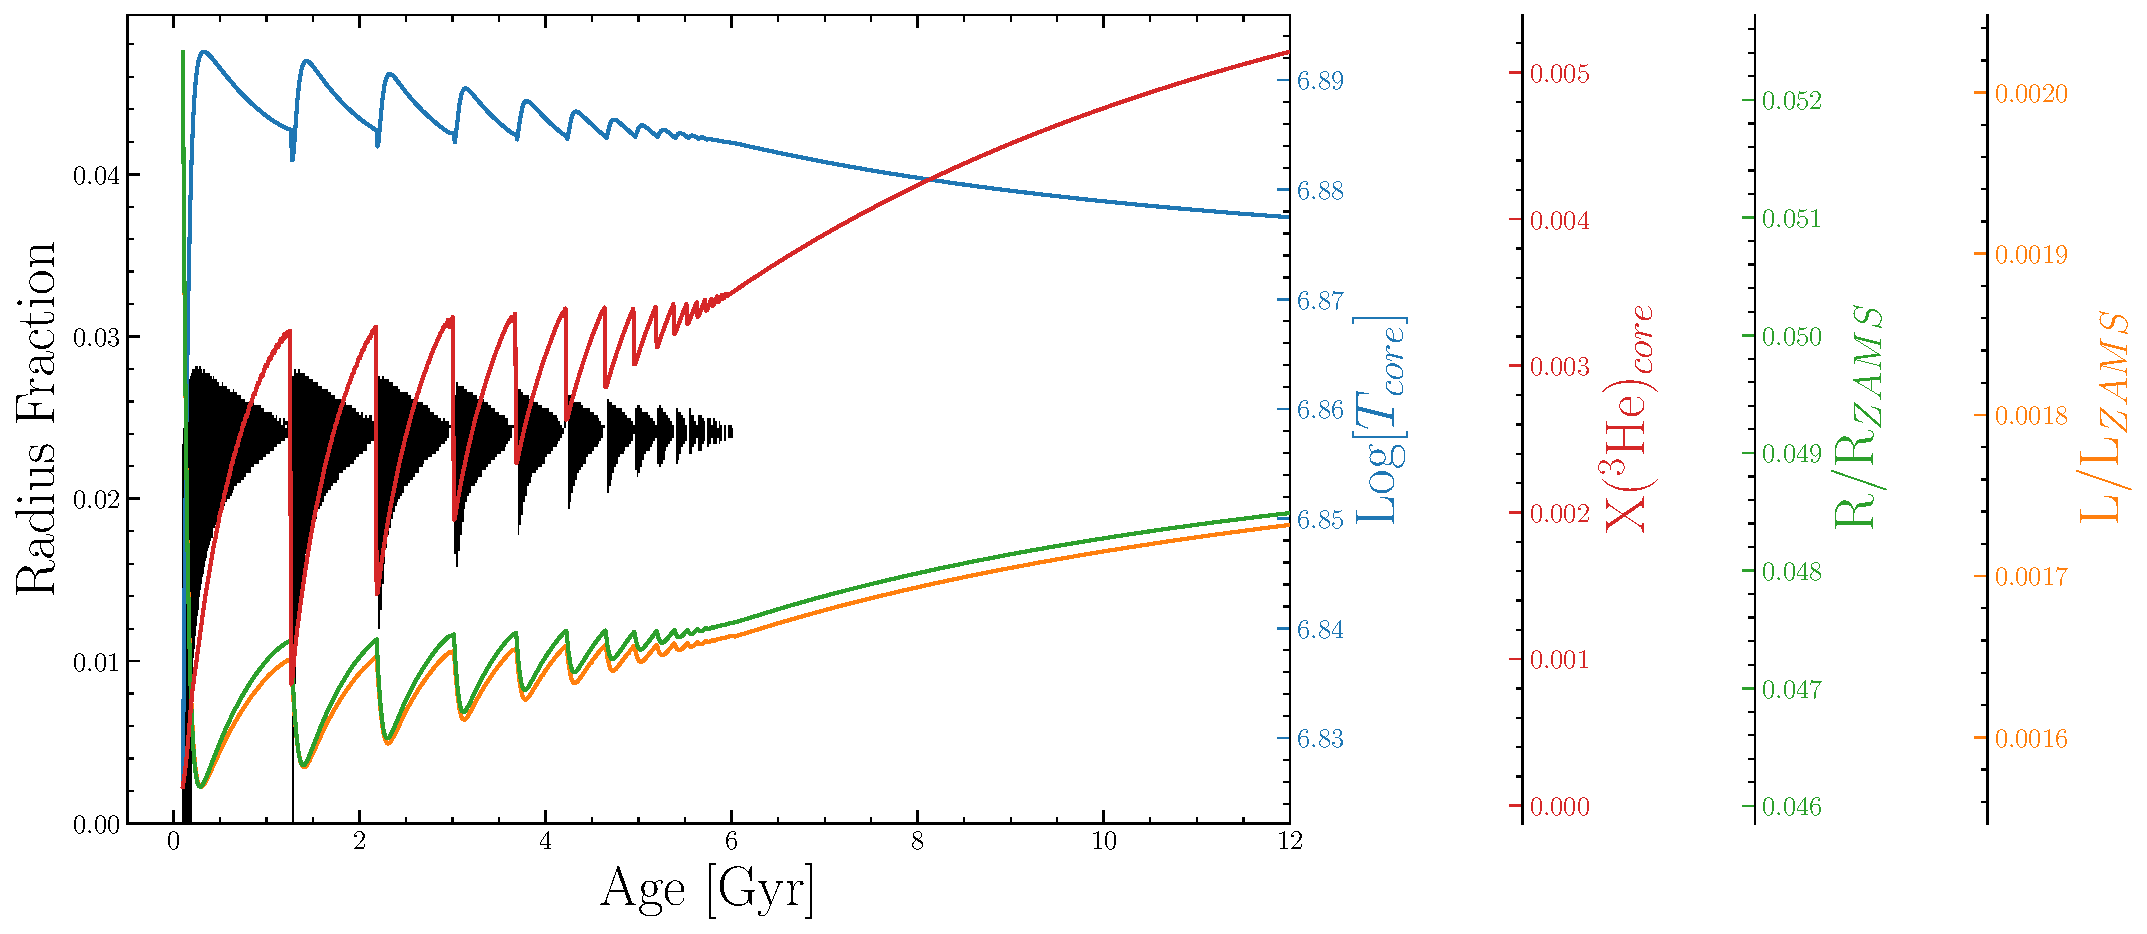
\includegraphics[width=0.9\textwidth]{figures/jaoMagActivity/Kippenhan_clamped.pdf}
  \caption{Kippenhan-Iben diagram for a 0.345 solar mass star. Note the
  periodic mixing events (where the plotted curves peak).}
  \label{fig:kippenhan}
\end{figure*}

Each synthetic star is assigned some base magnetic activity ($B_{0} \sim
\mathcal{N}(1, \sigma_{B})$) and then the number of mixing events before some age $t$
are counted based on local maxima in the core temperature. The toy magnetic
activity at age $t$ for the model is given in Equation \ref{eqn:activity}. An
example of the magnetic evolution resulting from this model is given in Figure
\ref{fig:simpleB}. Fundamentally, this model presents magnetic
activity variation due to mixing events as a random walk and therefore results will
increasing divergence over time.

\begin{align}\label{eqn:activity}
  B(t) = B_{0} + \sum_{i}B_{i} \sim \mathcal{N}(1, \sigma_{B}) 
\end{align}

\begin{figure}
  \centering
  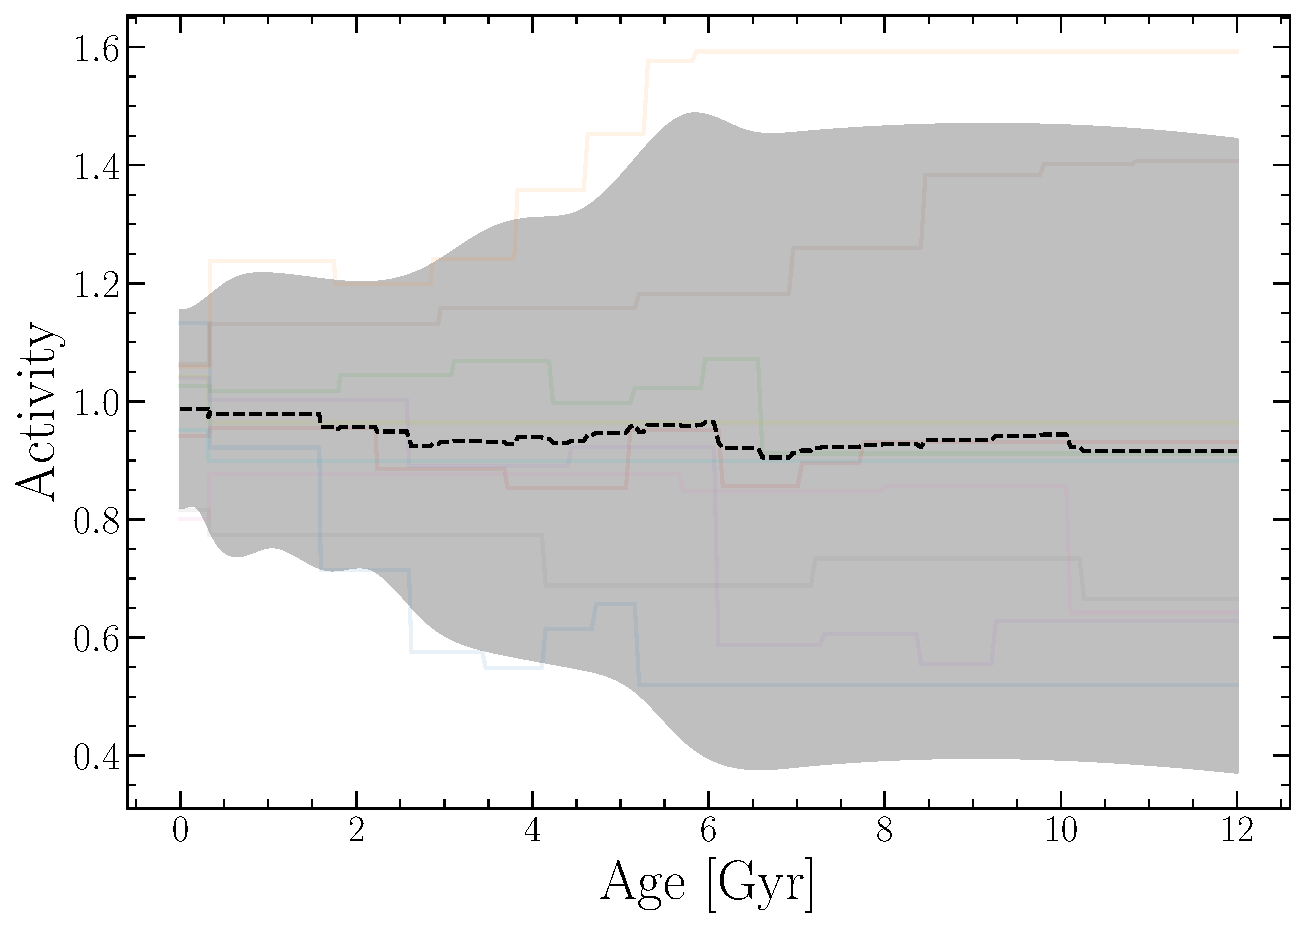
\includegraphics[width=0.85\textwidth]{figures/jaoMagActivity/simpleBEvolution.pdf}
  \caption{Example of the toy model presented here resulting in increased
  divergence between stars magnetic fields. The shaded region represents the
  maximum spread in the two point correlation function at each age.}
  \label{fig:simpleB}
\end{figure}

Applying the same analysis to these models as was done to the observations as
described in Section \ref{sec:results} we find that this simple model results
in a qualitatively similar trend in the standard deviation vs. Magnitude graph
(Figure \ref{fig:model}). In order to reproduce the approximately 50 percent
change to the spread of the activity metric observed in the combined dataset in
section \ref{sec:results} a distribution with a standard deviation of 0.1 is
required when sampling the change in the magnetic activity metric at each
mixing event. This corresponds to 68 percent of mixing events modifying the
activity strength by 10 percent or less. The interpretation here is important:
what this qualitative similarity demonstrates is that it may be reasonable to
expect kissing instabilities to result in the observed increased star-to-star
variation. Importantly, we are not able to claim that kissing instabilities
\textit{do} lead to these increased variations, only that they reasonably
could. Further modeling, observational, and theoretical efforts will be needed
to more definitively answer this question.

\begin{figure}
  \centering
  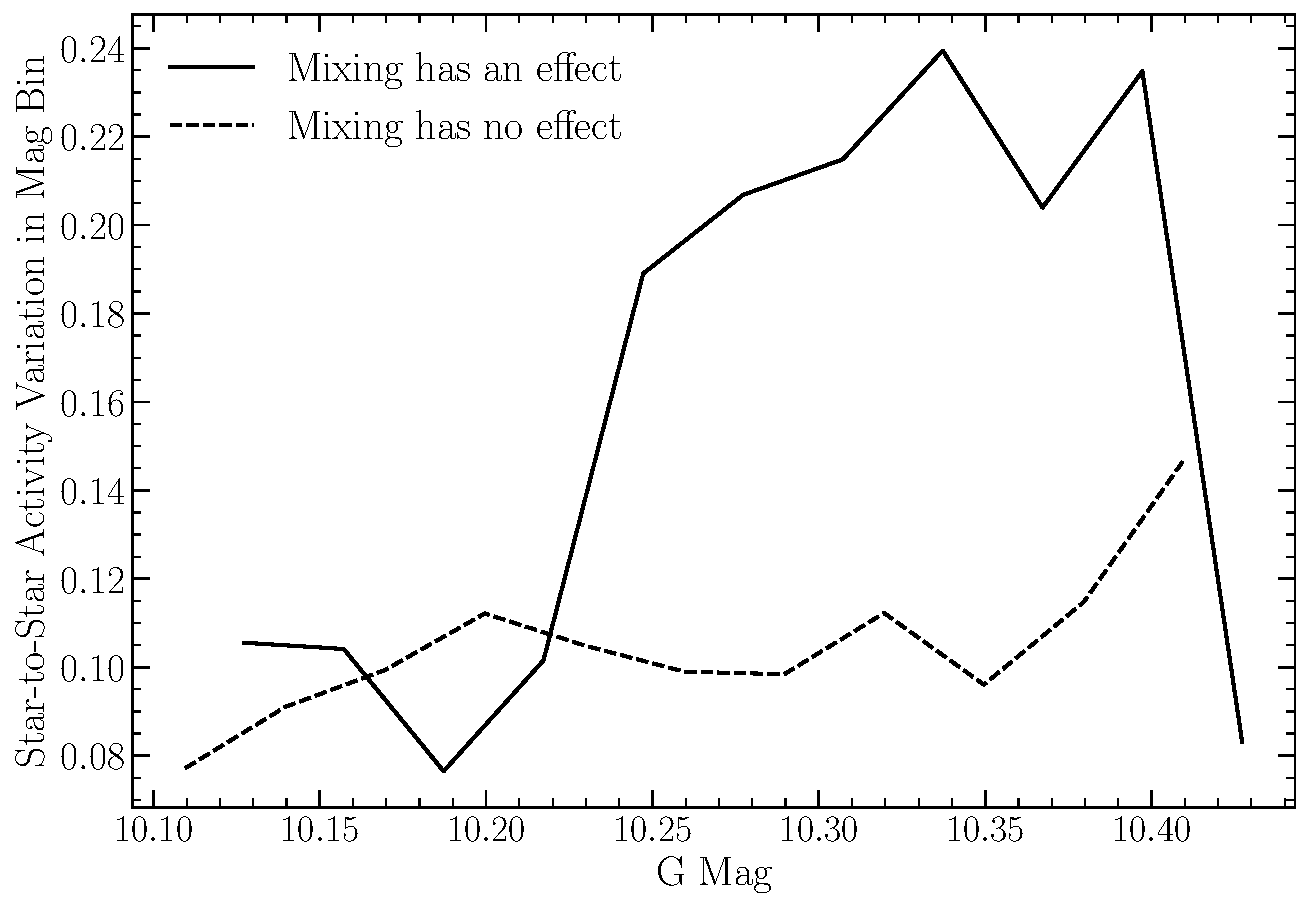
\includegraphics[width=0.85\textwidth]{figures/jaoMagActivity/SpreadModel.pdf}
  \caption{Toy model results showing a qualitatively similar discontinuity in the star-to-star magnetic activity variability.}
  \label{fig:model}
\end{figure}

\subsection{Limitations}
The model presented in this paper is very limited and it is important to keep
these limitations in mind when interpreting the results presented here. Some of
the main challenges which should be leveled at this model are the assumption
that the magnetic field will be altered by some small random perturbation at
every mixing event. This assumption was informed by the large number of free
parameters available to a physical star during the establishment of a large
scale magnetic field and the associated likely stochastic nature of that
process. However, it is similarly believable that the magnetic field will tend
to alter in a uniform manner at each mixing event. For example, since
differential rotation is generally proportional to the temperature gradient
within a star and activity is strongly coupled to differential rotation then it
may be that as the radiative zone reforms over thermal timescales the
homogenization of angular momentum throughout the star results in overall lower
amounts of differential rotation each after mixing event than would otherwise
be present.

Moreover, this model does not consider how other degenerate sources of magnetic
evolution such as stellar spin down, relaxation, or coronal heating may effect
star-to-star variability. These could conceivably lead to a similar increase in
star-to-star variability which is coincident with the Jao Gap magnitude as the
switch from fully to partially convective may effect efficiency of these
process.

Additionally, there are challenges with this toy model that originate from the
stellar evolutionary model. Observations of the Jao Gap show that the feature
is not perpendicular to the magnitude axis; rather, it is inversely
proportional to the color. No models of the Jao Gap published at the time of
writing capture this color dependency and \textit{what causes this color
dependency} remains one of the most pressing questions relating to the
underlying physics. This non captured physics is one potential explanation for
why the magnitude where our model predicts the increase in variability is not
in agreement with where the variability jump exists in the data.

Finally, we have not considered detailed descriptions of the dynamos of stars.
The magneto-hydrodynamical modeling which would be required to model the
evolution of the magnetic field of these stars at thermal timescale resolutions
over gigayears is currently beyond the ability of practical computing.
Therefore future work should focus on limited modeling which may inform the
evolution of the magnetic field directly around the time of a mixing event.

\section{Chemical Consistency}\label{sec:const}
There are three primary areas in which must the stellar models must be made
chemically consistent: the atmospheric boundary conditions, the opacities, and
interior abundances. The interior abundances are relatively easily handled by
adjusting parameters within our stellar evolutionary code. However, the other
two areas are more complicated to bring into consistency. Atmospheric boundary
conditions and opacities must both be calculated with a consistent set of
chemical abundances outside of the stellar evolution code.
{\bf Nearly all prior efforts at modeling multiple stellar populations in
globular clusters have adjusted the abundances used in the atmospheric interior
models, and in the high temperature opacities, but have not self-consistently
modified the corrosponding low-temperature opacities and surface bounary
conditions, as these are found from stellar atmosphere codes, and not the
stellar interior codes which are used to create stellar models and isochrones.
In this work, as in Dotter (2016), the stellar interior models are chemically
self-consistent with the stellar atmosphere models.} For evolution we The Dartmouth Stellar
Evolution Program (DSEP) \citep{Dotter2008}, a well tested 1D stellar evolution
code which has a particular focus on modelling low mass stars ($\le 2$
M$_{\odot}$)

\subsection{Atmospheric Boundary Conditions}\label{sec:atm}
Certain assumptions, primarily that the radiation field is at equilibrium and
radiative transport is diffusive \citep{Salaris2005}, made in stellar structure
codes, such as DSEP, are valid when the optical depth of a star is large.
However, in the atmospheres of stars, the number density of particles drops low
enough and the optical depth consequently becomes small enough that these
assumptions break down, and separate, more physically motivated, plasma
modeling code is required. Generally structure code will use tabulated
atmospheric boundary conditions generated by these specialized codes, such as ATLAS9
\citep{Kurucz1993}, PHOENIX \citep{Husser2013}, MARCS \citep{Gustafsson2008},
and MPS-ATLAS \citep{Kostogryz2023}. Often, as the boundary conditions are
expensive to compute, they are not updated as interior abundances vary. 

One key element when chemically consistently modeling NGC 2808 modeling is the
incorporation of new atmospheric models with the same elemental abundances as
the structure code. We use atmospheres generated from the \texttt{MARCS} grid
of model atmospheres \citep{Plez2008}. \texttt{MARCS} provides one-dimensional,
hydrostatic, plane-parallel and spherical LTE atmospheric models
\citep{Gustafsson2008}. Model atmospheres are made to match the
spectroscopically measured elemental abundances of populations A and E.
Moreover, for each population, atmospheres with various helium mass fractions
are generated. These range from Y=0.24 to Y=0.36 in steps of 0.03. All
atmospheric models are computed to an optical depth of $\tau = 100$ where their
temperature and pressures serves as boundary conditions for the structure code.
In general, enhancing helium in the atmosphere has only a small impact on the atmospheric
temperature profile, while leading to a drop in the pressure by $\sim 10 - 20 \%$.

\subsection{Opacities}\label{sec:opac}
In addition to the atmospheric boundary conditions, both the high and low
temperature opacities used by DSEP must be made chemically consistent. Here we
use OPLIB high temperature opacity tables \citep{Colgan2016} retrieved using
the TOPS web-interface. Retrival of High termperature opacities is done using
\texttt{pyTOPSScrape}, first introduced in \citet{Boudreaux2023}. Low
temperature opacity tables are retrieved from the Aesopus 2.0 web-interface
\citep{Marigo2009, Marigo2022}. Ideally, these opacities would be the same used
in the atmospheric models. However, the opacities used in the MARCS models are
not publicly available. As such, we use the opacities provided by the TOPS and
Aesopus 2.0 web-interfaces.

\section{fidanka}\label{sec:fidanka}
When fitting isochrones to the clusters with multiple populations we have four
main criteria for any method

\begin{itemize}
  \item The method must be robust enough to work along the entire main
    sequence, turn off, and much of the subgiant and red giant branch.
	\item Any method should consider photometric uncertainty in the fitting process.
	\item The method should be model independent, weighting any n number of populations equally.
	\item The method should be automated and require minimal intervention from the user.
\end{itemize}


We do not believe that any currently available software is a match for
our use case. Therefore, we elect to develop our own software suite, \fidanka.
\fidanka is a python package designed to automate much of the process of
measuring fiducial lines in CMDs, adhering to the four criteria we lay out
above. Primary features of \fidanka may be separated into three
categories: fiducial line measurement, stellar population synthesis, and
isochrone optimization/fitting. Additionally, there are utility functions that
are detailed in the \fidanka documentation.

\subsection{Fiducial Line Measurement}
\fidanka takes a iterative approach to measuring fiducial lines, the first step
of which is to make a ``guess'' as to the fiducial line. This initial guess
is calculated by splitting the CMD into magnitude bins, with uniform numbers of
stars per bin (so that bins are cover a small magnitude range over densely
populated regions of the CMD while covering a much larger magnitude range in
sparsely populated regions of the CMD, such as the RGB). A unimodal Gaussian
distribution is then fit to the color distribution of each bin, and the
resulting mean color is used as the initial fiducial line guess. This rough
fiducial line will approximately trace the area of highest density. The initial
guess will be used to verticalze the CMD so that further algorithms can work in
1-D magnitude bins without worrying about weighting issues caused by varying
projections of the evolutionary sequence onto the magnitude axis.
Verticalization is preformed taking the difference between the guess fiducial
line and the color of each star in the CMD.

If \fidanka were to simply apply the same algorithm to the verticalized CMD
then the resulting fiducial line would likely be a re-extraction of the initial
fiducial line guess. To avoid this, we take a more robust, number density based
approach, which considers the distribution of stars in both color and magnitude
space simultaneously. For each star in the CMD we first use an
\texttt{introselect} partitioning algorithm to select the 50 nearest stars in
F814W vs. F275W-F814W space. To account for the case where the star is at an
extreme edge of the CMD, those 50 stars include the star itself (such that we
really select 49 stars + 1). We use
\texttt{qhull}\footnote{https://www.qhull.com}\citep{Barber1996} to calculate
the convex hull of those 50 points. The number density at each star then is
defined as $50/A_{hull}$, where $A_{hull}$ is the area of the convex hull.
Because we use a fixed number of points per star, and a partitioning algorithm
as opposed to a sorting algorithm, this method scales like $\mathcal{O}(n)$,
where n is the number of stars in the CMD. This method also intrinsically
weights the density of of each star equally as the counting statistics per bin
are uniform. We are left with a CMD where each star has a defined number
density (Figure \ref{densityMapDemo}).

\begin{figure*}
	\centering
	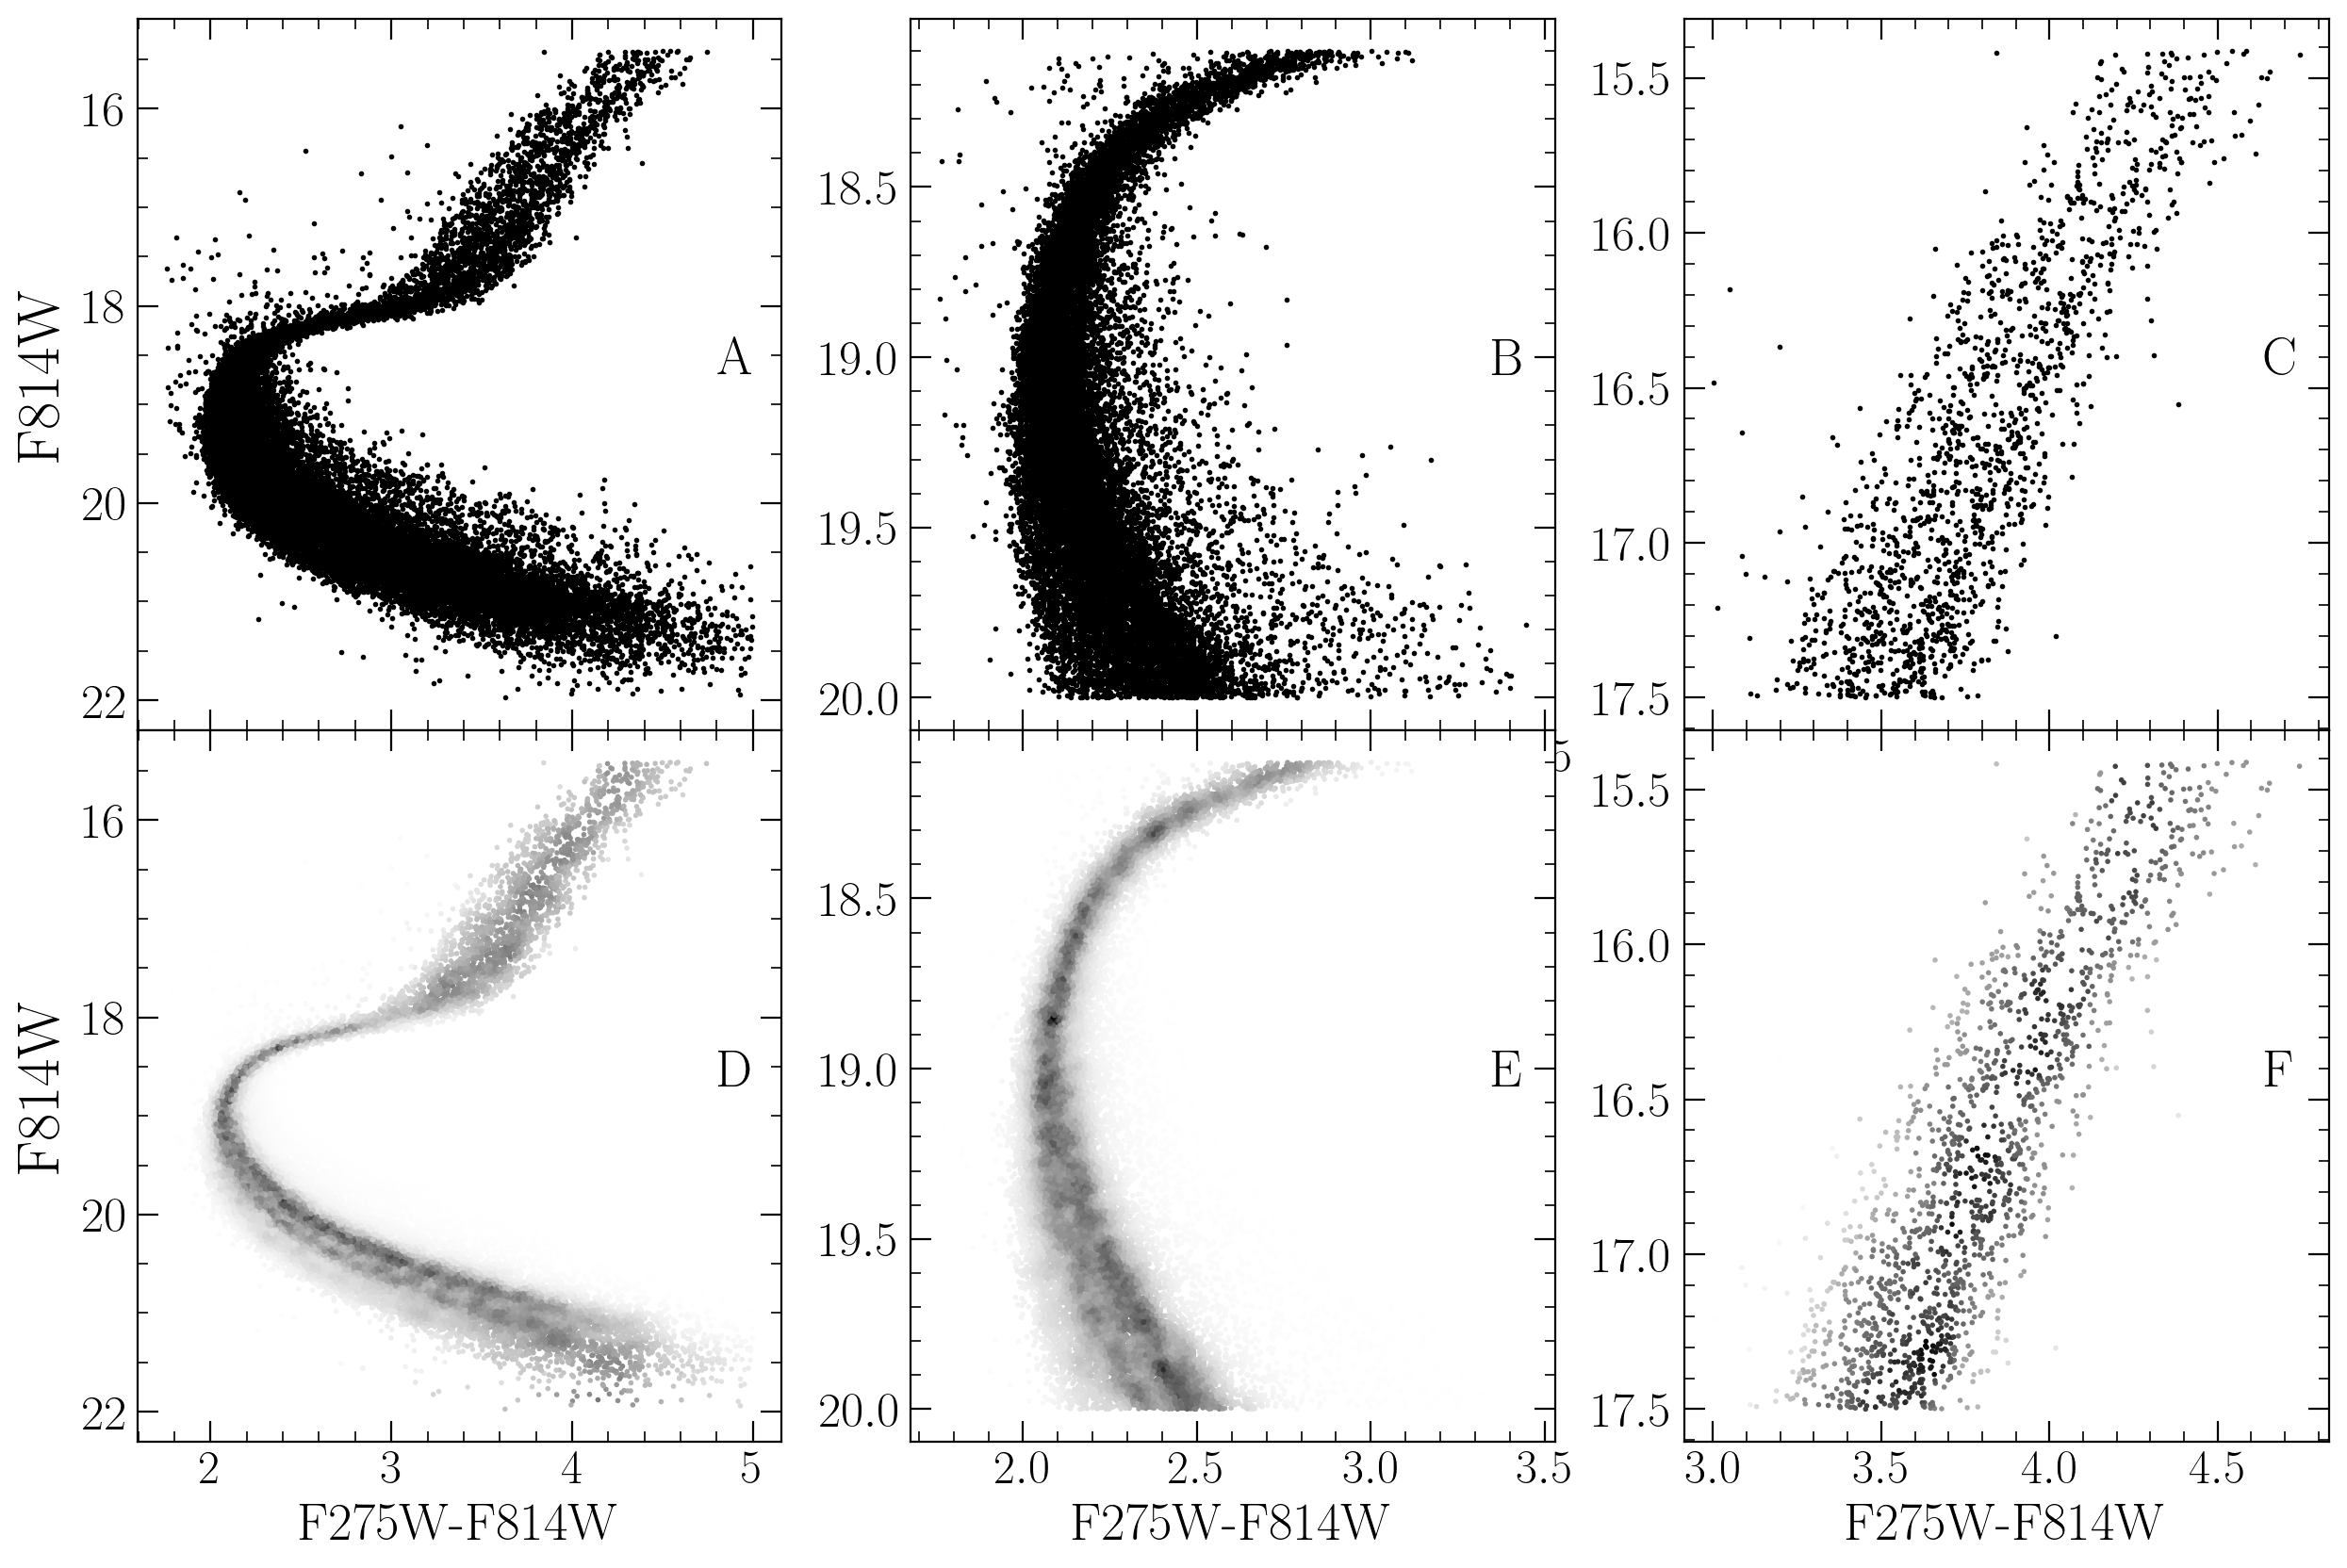
\includegraphics[width=0.9\textwidth]{figures/ngc2808/notebookFigures/DensityMapDemo.png}
  \caption{Figures in the top row are the raw CMD, while figures in the bottom
  row are colored by the density map.Density map demo showing density estimate
  over different parts of the evolutionary sequence. The left panel shows the
  density map over the entire evolutionary sequence, while the middle panel
  shows the density map over the main sequence and the right most panel shows
  the density map over the RGB. }
	\label{densityMapDemo}
\end{figure*}

\fidanka can now exploit this density map to fit a better fiducial line to the
data, as the density map is far more robust to outliers. There are multiple
algorithms we implement to fit the fiducial line to the color-density profile
in each magnitude bin (Figure \ref{densityBinsDemo}); they are explained in
more detail in the \fidanka documentation. However, of most relevance here is
the Bayesian Gaussian Mixture Modeling (BGMM) method. BGMM is a clustering
algorithm which, for some fixed number of n-dimensional Gaussian distributions,
$K$, determines the mean, covariance, and mixing probability (somewhat
analogous to amplitude) of each $k^{th}$ distribution, such that the local
lower bound of the likelyhood of each star belonging strongly to a single
distribution is maximized. 

\begin{figure}
	\centering
	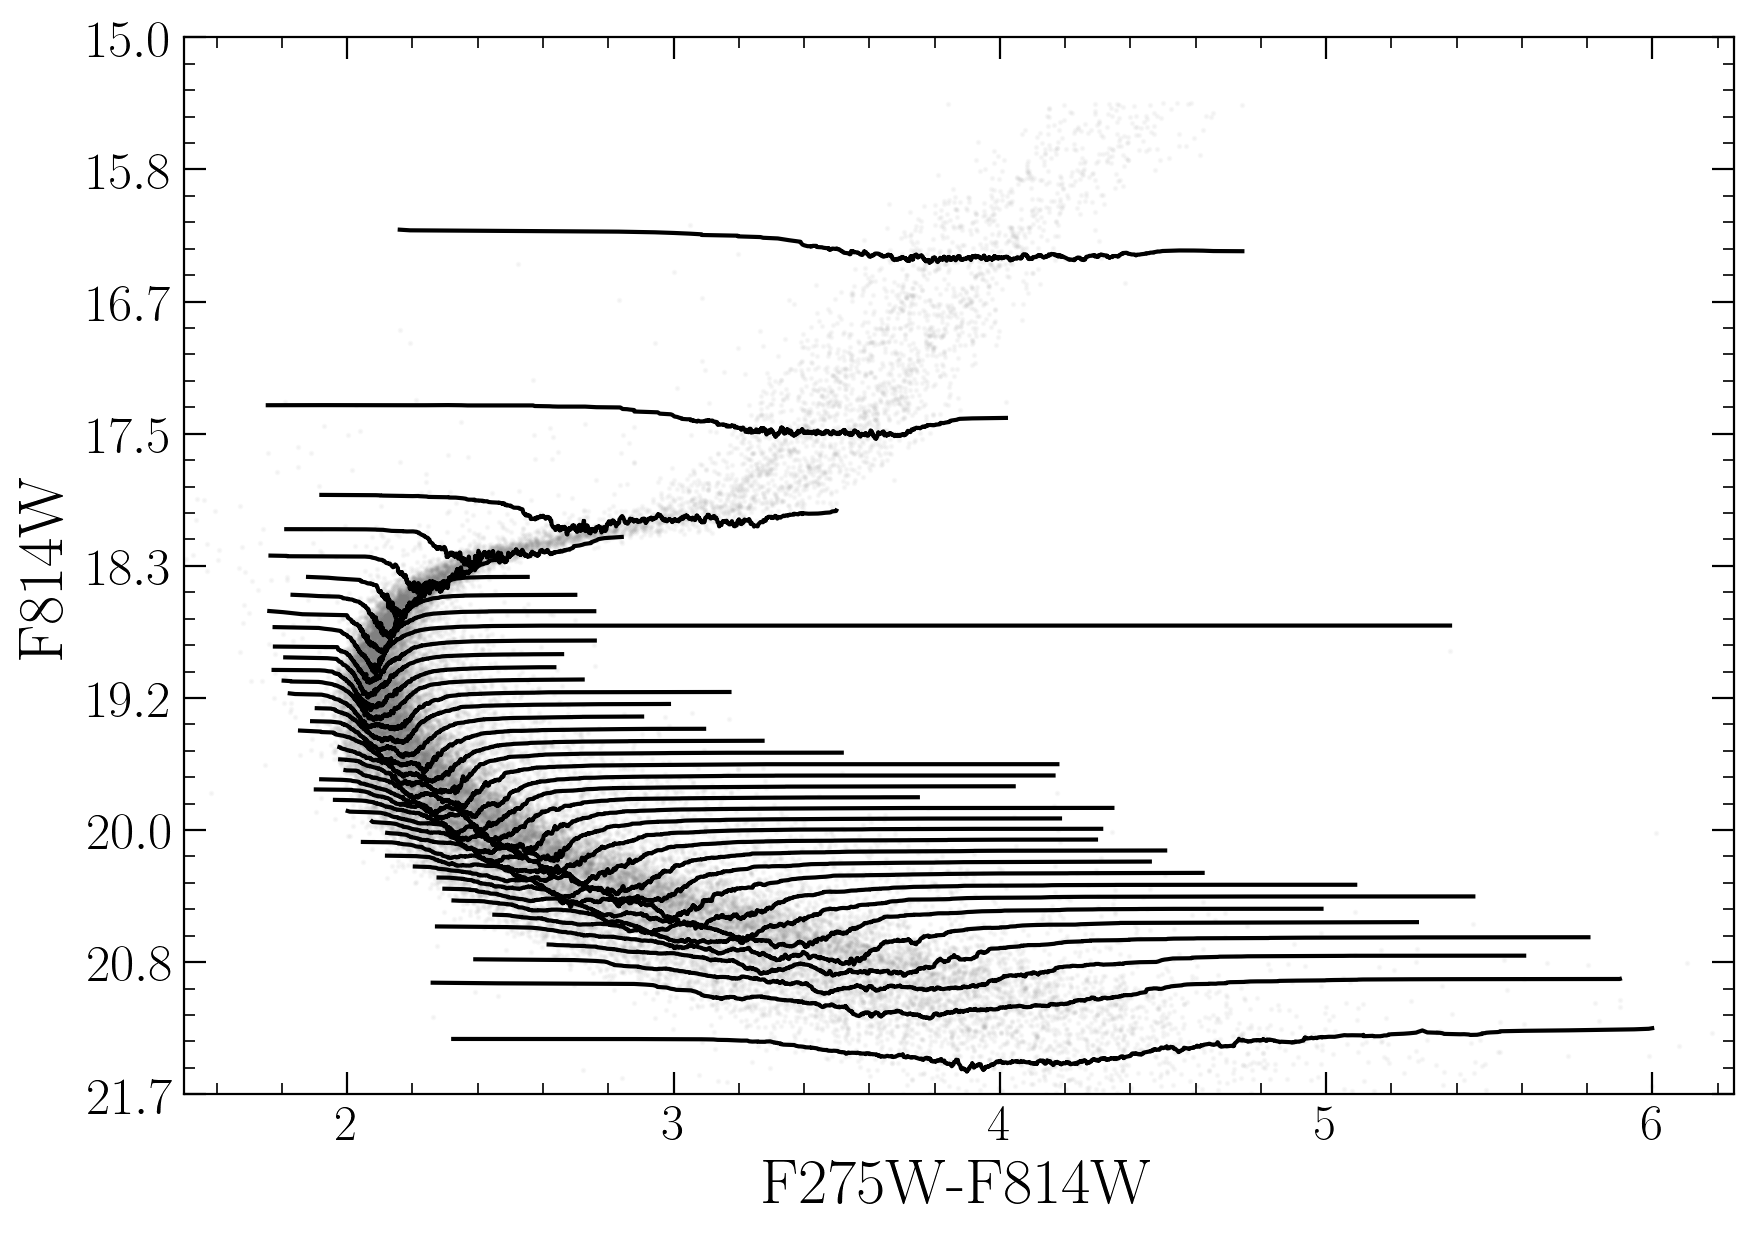
\includegraphics[width=0.85\textwidth]{figures/ngc2808/notebookFigures/DensityBinsDemo.png}
	\caption{CMD where point brightness is determined by local density. Lines show the
	density-color profile in each magnitude bin. In this figure adaptive
	binning targeted 1000 stars per bin}
	\label{densityBinsDemo}
\end{figure}

Maximization is preformed using the Dirichlet process, which is a
non-parametric Bayesian method of determining the number of Gaussian
distributions, $K$, which best fit the data \citep{Ferguson1973, scikit-learn}.
Use of the Dirichlet process allows for dynamic variation in the number of
inferred populations from magnitude bin to magnitude bin. Specifically,
populations are clearly visually separated from the lower main sequence through
the turn off; however, at the turn off and throughout much of the subgiant
branch, the two visible populations overlap due to their extremely similar ages
\citep[i.e.][]{Jordan2002}. The Dirichlet process allows for the BGMM method to
infer a single population in these regions, while inferring two populations in
regions where they are clearly separated. More generally, the use of the
Dirichlet process removes the need for a prior on the exact number of
populations to fit. Rather, the user specifies a upper bound on the number of
populations within the cluster. An example bin (F814W = 20.6) is shown in
Figure \ref{fig:BGMMDist}.

\begin{figure*}
	\centering
	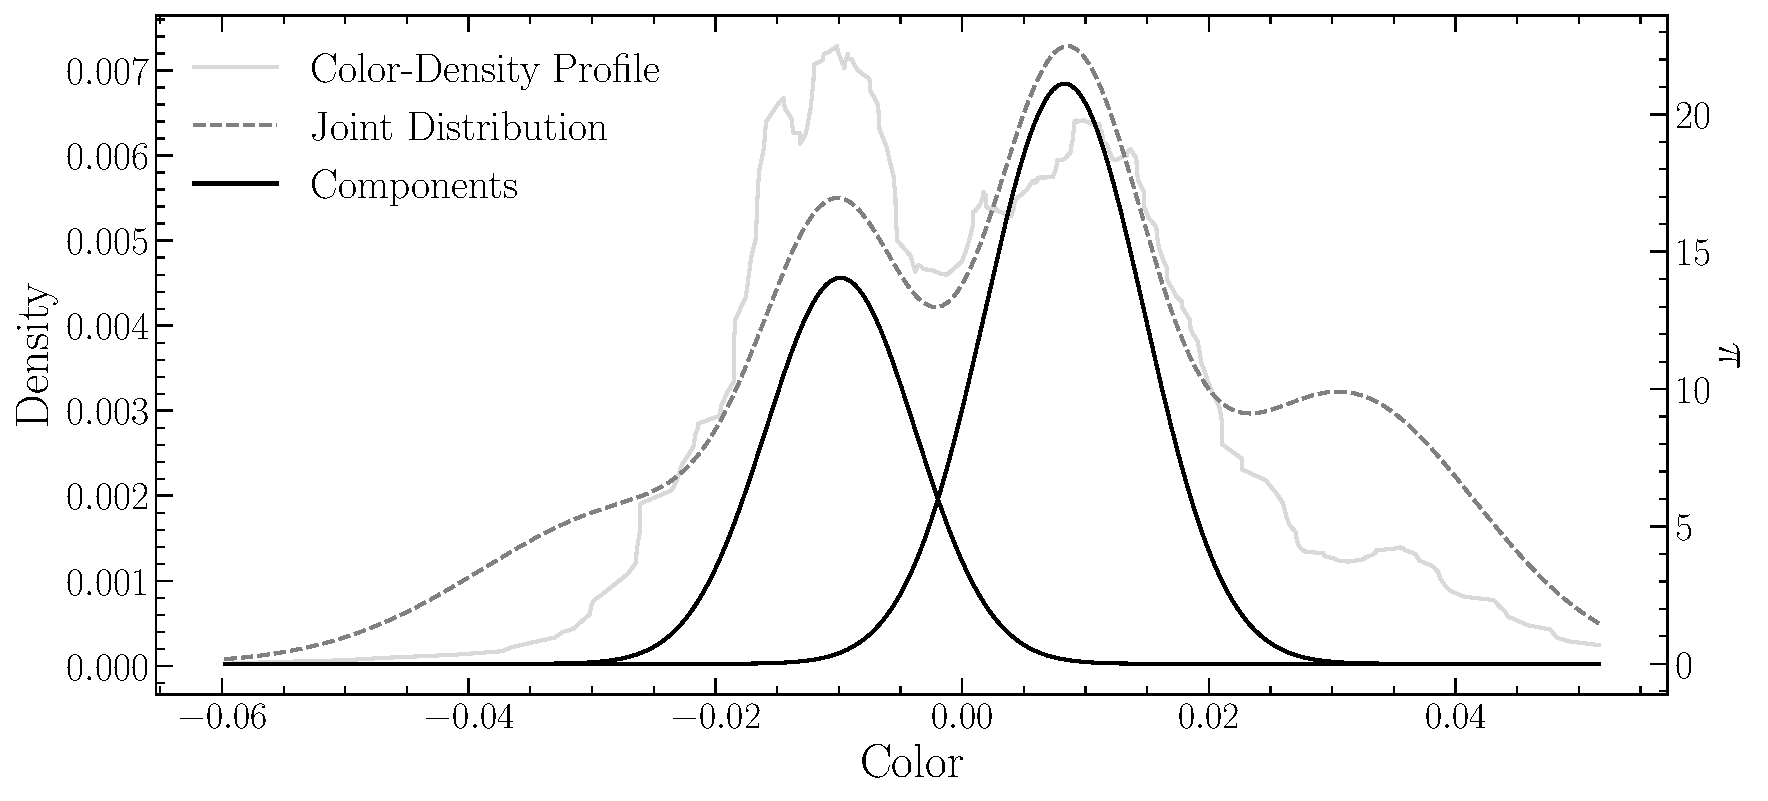
\includegraphics[width=0.9\textwidth]{figures/ngc2808/BGMMMixingBin.pdf}
	\caption{Example of BGMM fit to a magnitude bin. The grey line shows the
	underlying color-density profile, while the black dashed-line shows the
	joint distribution of each BGMM component. The solid black lines show the
	two selected components.}
	\label{fig:BGMMDist}
\end{figure*}

\fidanka's BGMM method first breaks down the verticalized CMD into magnitude
bins with uniform numbers of stars per bin (here we adopt 250). Any stars left
over are placed into the final bin. For each bin a BGMM model with a maximum of
5 populations is fit to the color density profile. The number of populations is
then inferred from the weighting parameter (the mixing probability) of each
population. If the weighting parameter of any $k^{th}$ components less than
{\color{blue}0.05}, then that component is considered to be spurious and
removed. Additionally, if the number of populations in the bin above and the
bin below are the same, then the number of populations in the current bin is
forced to be the same as the number of populations in the bin above. Finally,
the initial guess fiducial line is added back to the BGMM inferred line. Figure
\ref{fig:vertFit} shows the resulting fiducial line(s) in each magnitude bin
for both a verticalized CMD and a non verticalized CMD. In contrast to other
work in the literature where evidence for up to 5 distinct populations has been
found; we only find evidence for two stellar populations.

\begin{figure}
	\centering
	\includegraphics[width=0.65\textwidth]{figures/ngc2808/vertFit.png}
  \caption{Verticalized CMD (where the color of each data point is subtracted
  from the color of the fiducial line at that magnitude) where point brightness
  is determined by density (top). CMD where point brightness is determined by
  density, calculated fiducial lines are shown (bottom). The data used is from
  the Hubble Space Telescope UV Legacy Survey of Galactic Globular Clusters.}
	\label{fig:vertFit}
\end{figure}

This method of fiducial line extraction effectively discriminated between
multiple populations along the main sequence and RGB of a cluster, while
simultaneously allowing for the presence of a single population along the MSTO
and subgiant branch. 

We can adapt this density map based BGMM method to consider photometric
uncertainties by adopting a simple Monte Carlo approach. Instead of measuring
the fiducial line(s) a single time, \fidanka can measure the fiducial line(s)
many times, resampling the data with replacement each time. For each resampling
\fidanka adds a random offset to each filter based on the photometric
uncertainties of each star. From these $n$ measurements the mean fiducial line
for each sequence can be identified along with upper and lower bound confidence
intervals in each magnitude bin.

\subsection{Stellar Population Synthesis}
While not extensively used in this paper \fidanka can, in addition to measuring fiducial
lines, preform stellar population synthesise. \fidanka's population synthesis
module can generate synthetic stellar population from a set of MIST formatted
isochrones. This is of primary importance for binary population modeling. The
module is also used to generate synthetic CMDs for the purpose of testing the
fiducial line extraction algorithms against priors.

\fidanka uses MIST formatted isochrones \citep{Dotter2016} as input along
with distance modulus, B-V color excess, binary mass fraction, and bolometric
corrections. An arbitrarily large number of isochrones may be used to define an
arbitrary number of populations. Synthetic stars are samples from each
isochrone based on a definable probability (for example it is believed that
$\sim90\%$ of stars in globular clusters are younger population
\citep[e.g.][]{Suntzeff1996, Carretta2013}). Based on the metallicity, $\mu$, and E(B-V) of each
isochrone, bolometric corrections are taken from bolometric correction tables.
Where bolometric correction tables do not include exact metallicities or
extinctions a linear interpolation is preformed between the two bounding
values. 

\subsection{Isochrone Optimization}
The optimization routines in \fidanka will find the best fit distance modulus,
B-V color excess, and binary number fraction for a given set of isochrones. If
a single isochrone is provided then the optimization is done by minimizing the
$\chi^2$ of the perpendicular distances between an isochrone and a fiducial
line. If multiple isochrones are provided then those isochrones are first used
to run stellar population synthesis and generate a synthetic CMD. The
optimization is then done by minimizing the $\chi^2$ of both the perpendicular
distances between and widths of the observed fiducial line and the fiducial
line of the synthetic CMD.


\subsection{Fidanka Testing}
In order to validate fidanka we have run an series of injection recovery tests
using \fidanka's population synthesis routines to build various synthetic
populations and \fidanka's fiducial measurement routines to recover these
populations. Each population was generated using the initial mass function
given in \citep{Milone2012} for the redmost population ($\alpha=-1.2$).
Further, every population was given a binary population fraction of 10\%,
distance uniformly sampled between 5000pc and 15000pc, and a B-V color excess
uniformly sampled between 0 and 0.1. Finally, each synthetic population was
generated using a fixed age  uniformlly sampled between 7 Gyr and 14 Gyr. An
example synthetic population along with its associated best fit isochrone are
shown in Figure \ref{fig:ValidationBestFit}.

\begin{figure}
  \centering
  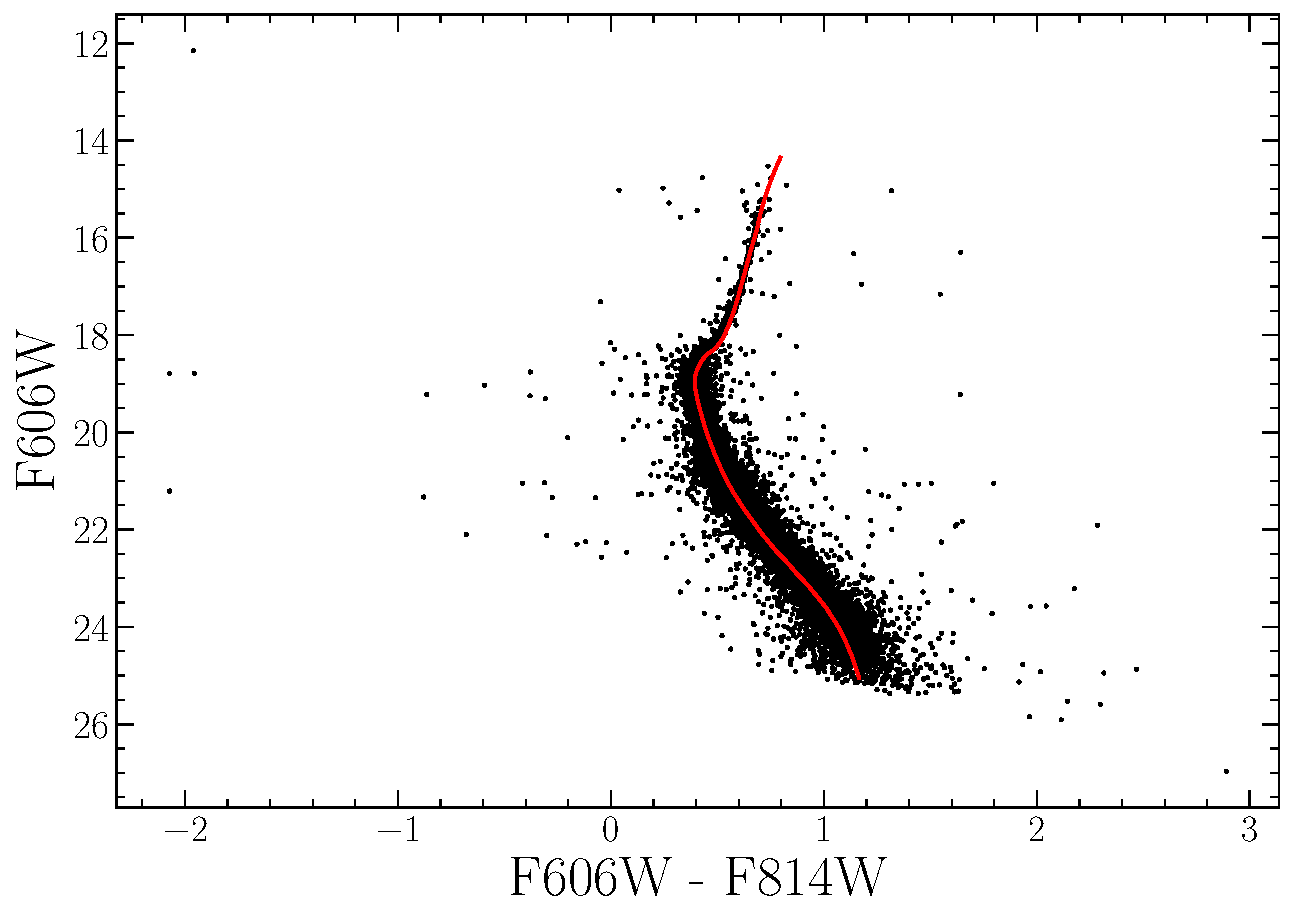
\includegraphics[width=0.85\textwidth]{figures/ngc2808/ExtractedIsoFit.pdf}
  \caption{Synthetic population generated by fidanka at 10000pc with E(B-V) =
  0, and an age of 12 Gyr along with the best fitting isochrone. The best fit
  paremeters are derived to be $mu=15.13$, E(B-V)=0.001, and an age of 12.33
  Gyr.}
  \label{fig:ValidationBestFit}
\end{figure}

For each trial we use \fidanka to measure the fiducial line and then optimize
that fiducial line against the originating isochrone to esimate distance
modulus, age, and color B-V excess. Figure \ref{fig:validationDist} is built
from 1000 Monte-Carlo trials and shows the mean and width of the percent
error distributions for $\mu$, $A_{v}$, and age. In general \fidanka is able to
recover distance modulii effectively with age and E(B-V) reovery falling in
line with other literature that does not cosider the CMD outside of the main
sequence, main sequence turn off, sub giant, and red giant branches;
specifically, it should be noted that \fidanka is not setup to model the
horizontal branch.

\begin{figure}
  \centering
  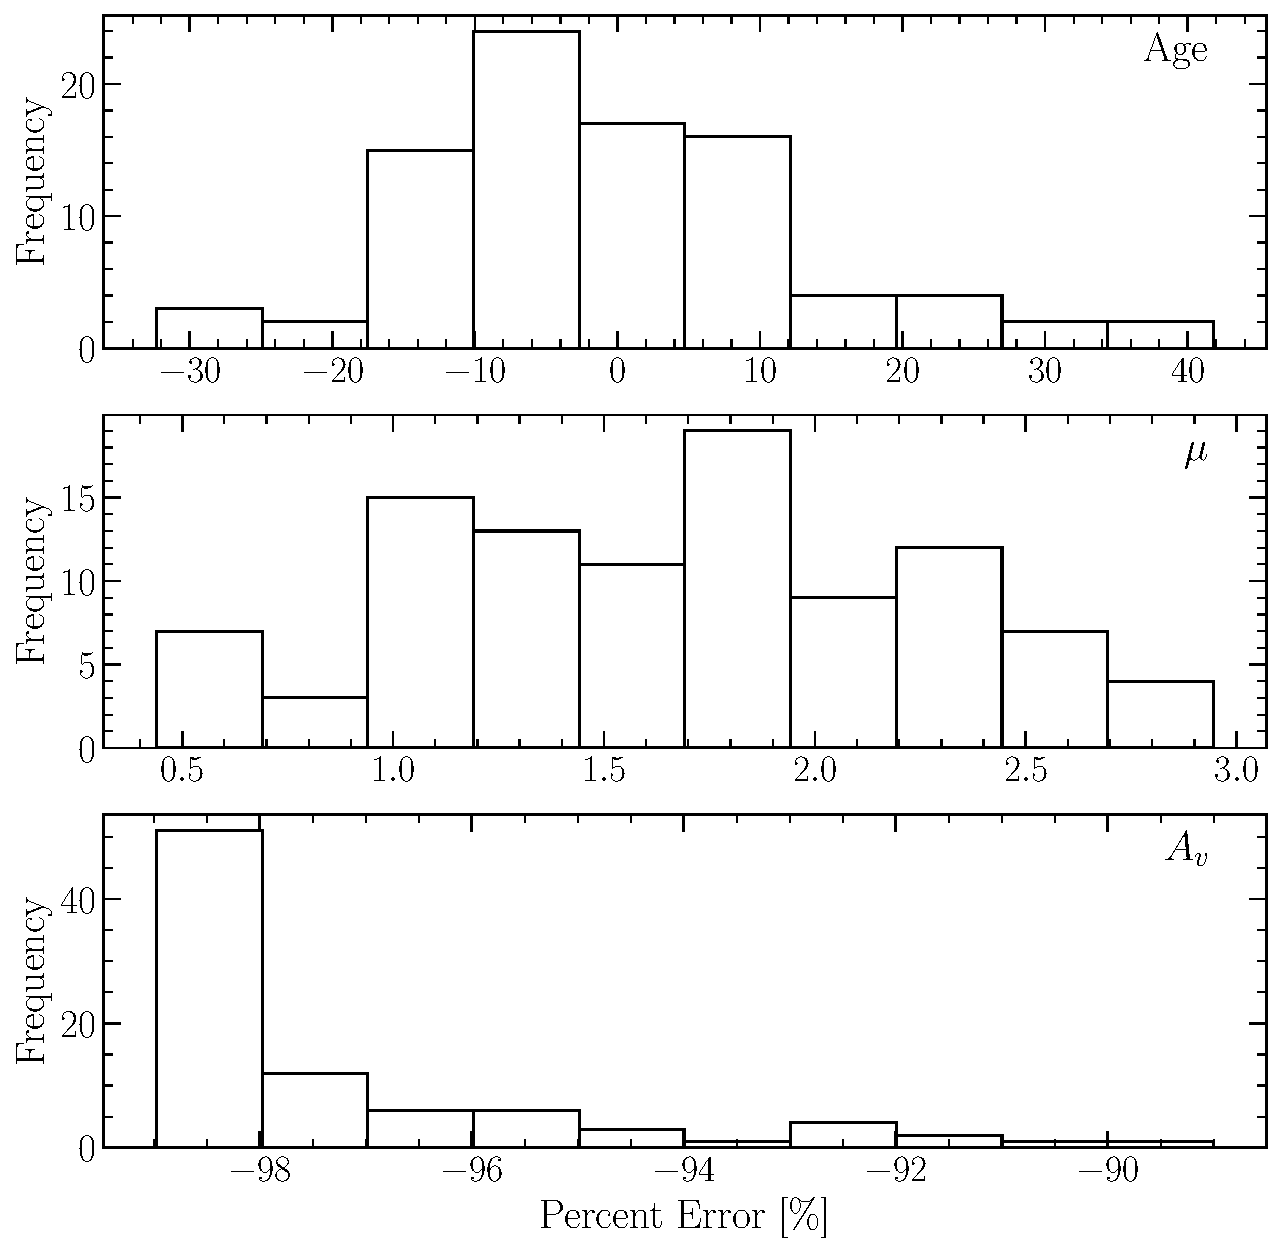
\includegraphics[width=0.85\textwidth]{figures/ngc2808/DistributionOfErrors.pdf}
  \caption{Percent Error distribution for each of the three deriver parameters.
  Note that these values will be sensitive to the magnitude uncertainties of
  the photometry. Here we made use of the ACS artificial star tests to estimate
  the uncertanties.}
  \label{fig:validationDist}
\end{figure}

\section{Isochrone Fitting}\label{sec:isoFit}
We fit pairs of isochrones to the HUGS data for NGC 2808 using \fidanka, as
descrbed in \S \ref{sec:fidanka}. Two isochrones, one for Population
A and one for Population E are fit simultaneously. These isochrones are
constrained to have distance modulus, $\mu$, and color excess, E(B-V) which
agree to within 1\%. Moreover, we constrain the mixing length, $\alpha_{ML}$, for any two isochrones in a set to be within 0.5 of one and other. For every isochrone in the
set of combination of which fulfilling these constraints $\mu$, $E(B-V)$,
Age$_{A}$, and $Age_{B}$ are optimized to reduce the $\chi^{2}$ distance
between the fiducial lines and the isochrones. Because we fit fiducial lines
directly, we do not need to consider the binary population fraction, $f_{bin}$,
as a free parameter.

The best fit isochrones are shown in Figure \ref{fig:BestFitResults} and optimized
parameters for these are presented in Table \ref{tab:BestFitResults}. We find helium mas fractions which are consistent with those identified in past literature \citep[e.g.][]{Milone2015}. Note that our helium mass fraction gird has a spacing of 0.03 between grid points and we are therefore unable to resolve between certain proposed helium mass fractions for the younger sequence (for example between 0.37 and 0.39).

\begin{figure*}
  \centering
  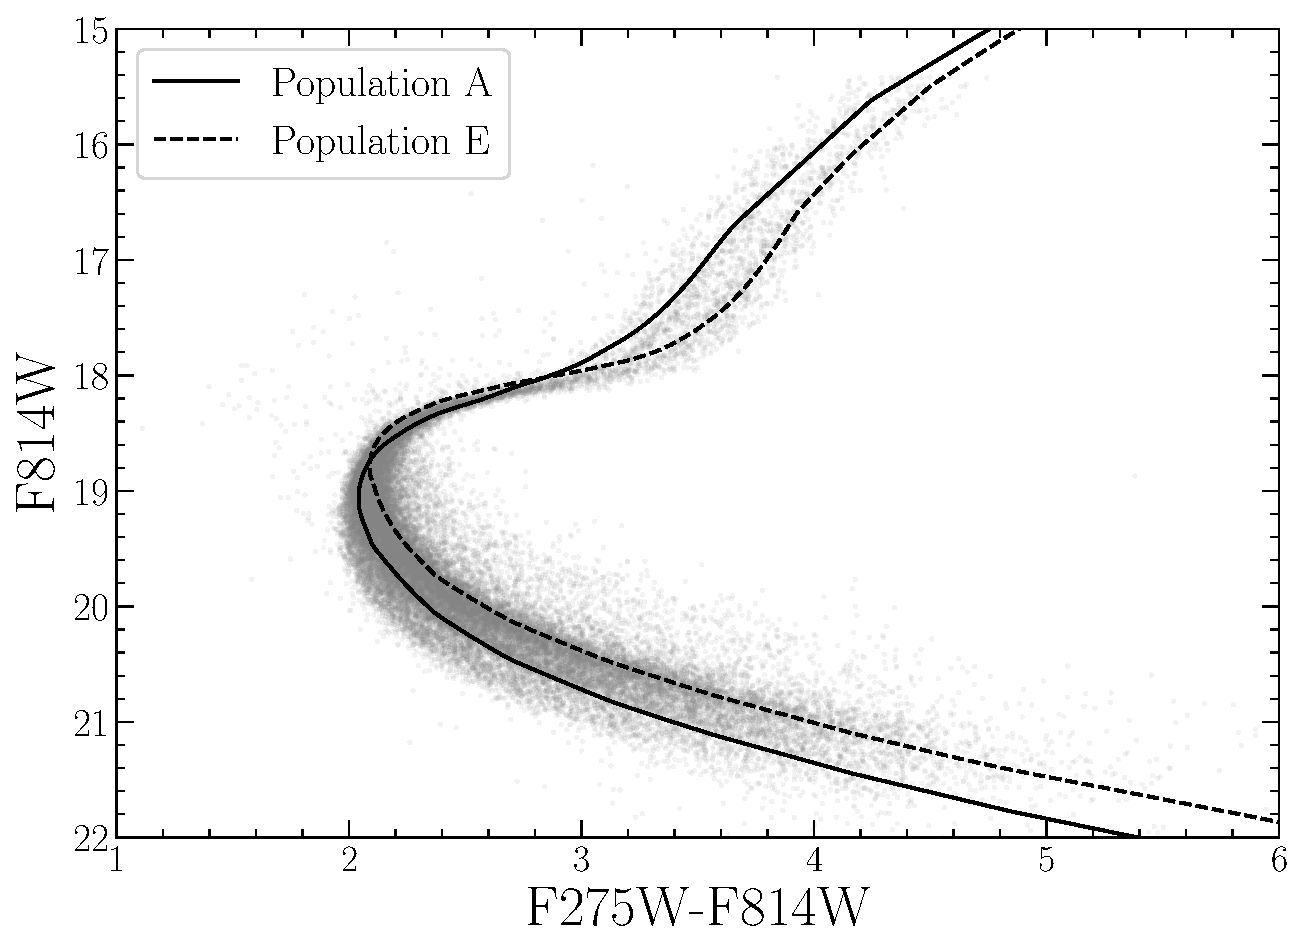
\includegraphics[width=0.9\textwidth]{figures/ngc2808/BestFitResults.pdf}
  \label{fig:BestFitResults}
  \caption{Best fit isochrone results for NGC 2808.}
\end{figure*}

\begin{table*}
  \centering
  \begin{tabular}{c | c c c c c c}
    \hline
    population & age & distance modulus & extinction & Y & $\alpha_{ML}$ & $\chi^{2}_{\nu}$\\
    & [Gyr] & & [mag] & & &\\
    \hline
    \hline
    A & 12.3 & 14.91 & 0.54 & 0.24 & 1.901 & 0.014\\
    E & 14.3 & 14.96 & 0.54 & 0.39 & 1.750 & 0.017 \\
    \hline
  \end{tabular}
  \label{tab:BestFitResults}
  \caption{Best fit parameters derived from fitting isochrones to the fiducual lines derived from the NCG 2808 photometry.}
\end{table*}


Past literature \citep[e.g. ][]{Milone2015, Milone2018} have found helium mass fraction variation from the low redmost to bluemost populations of $\sim 0.12$. Here we find a helium mass fraction variation of 0.15 which, given the spacing of the helium grid we use \textbf{is consistent with these past results}.

\subsection{The Number of Populartions in NGC 2808}
In order to estimate the number of populations which ideally fit the NGC 2808
F275W-F814W photometry without overfitting the data we make use of silhouette
analysis \citep[][and in a similar manner to how \citet{Valle2022}
preform their analysis of spectroscopic data]{ROUSSEEUW198753}. We find the average silhouette score for all tagged
clusters identified using BGMM in all magnitude bins over the CMD using the
standar python module \texttt{sklearn}. Figure \ref{fig:clusterAn} shows the
silhouette analysis results and that 2 populations fit the photometry most
ideally. This is in line with what our BGMM model predicts for the majority of
the the CMD.

\begin{figure}
  \centering
  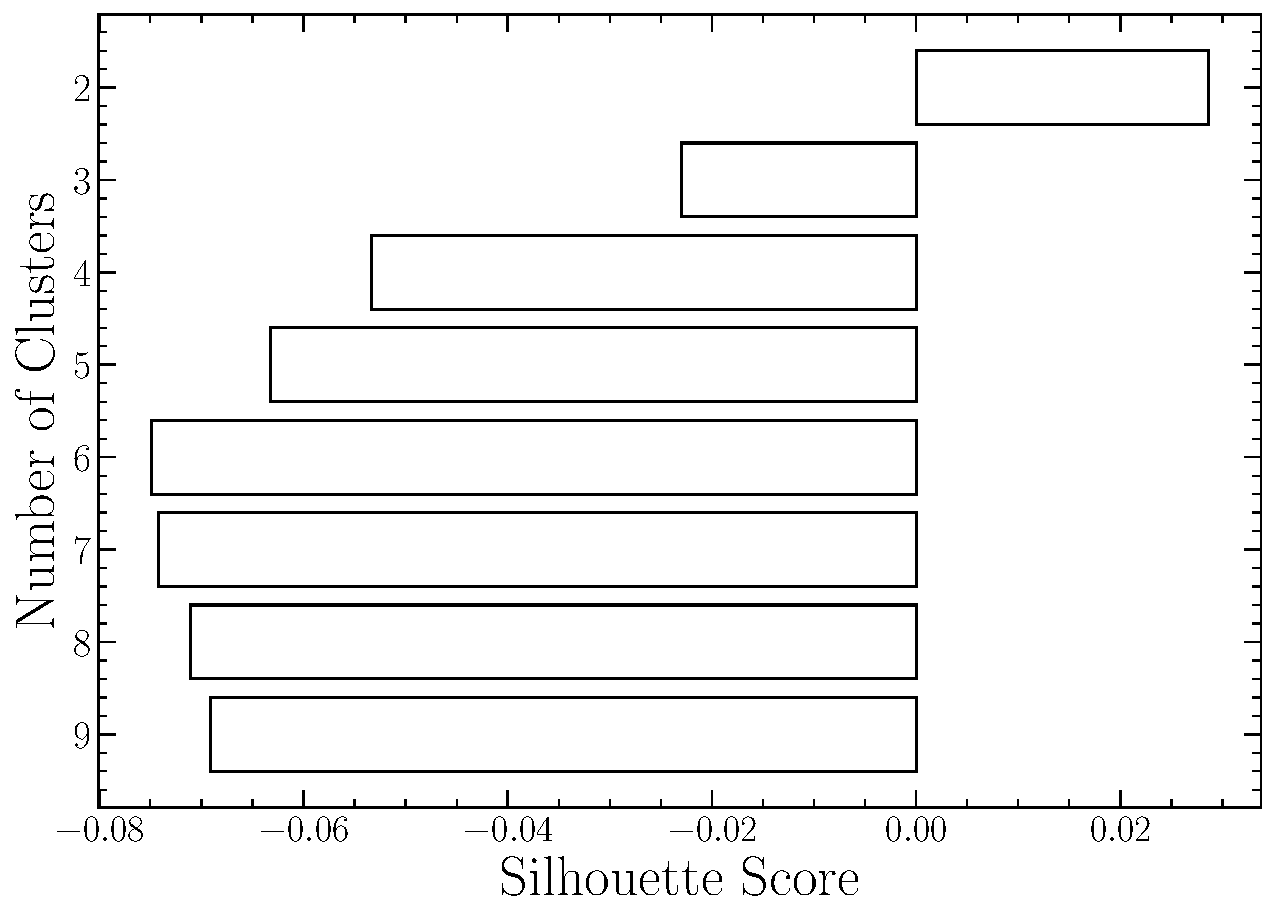
\includegraphics[width=0.45\textwidth]{figures/ngc2808/ClusterAnalysis.pdf}
  \caption{Silhouette analysis for NGC 2808 F275W-F814W photometry. The Silhouette scores
  are an average of score for each magnitude bin. Positive scores incidate that the clustering
  algorithm produced well distinguised clusters while negative scores indicate clusters which are not
  well distinguised.}
  \label{fig:clusterAn}
\end{figure}


\subsection{ACS-HUGS Photometric Zero Point Offset}
The Hubble legacy archive photometry used in this work is calibrated to the
Vega magnitude system. However, we have found that the photometry has a
systematic offset of $\sim0.026$ magnitudes in the F814W band when
compared to the same stars in the ACS survey (Figure \ref{fig:offset}). The
exact cause of this offset is unknown, but it is likely due to a difference in
the photometric zero point between the two surveys. A full correction of this
offset would require a careful re-reduction of the HUGS photometry, which is
beyond the scope of this work. We instead recognize a 0.02 inherent uncertainty
in the inferred magnitude of any fit when comparing to the ACS survey. This
uncertainty is small when compared to the uncertainty in the
distance modulus and should not affect the conclusion of this
paper. 

\begin{figure*}
  \centering
  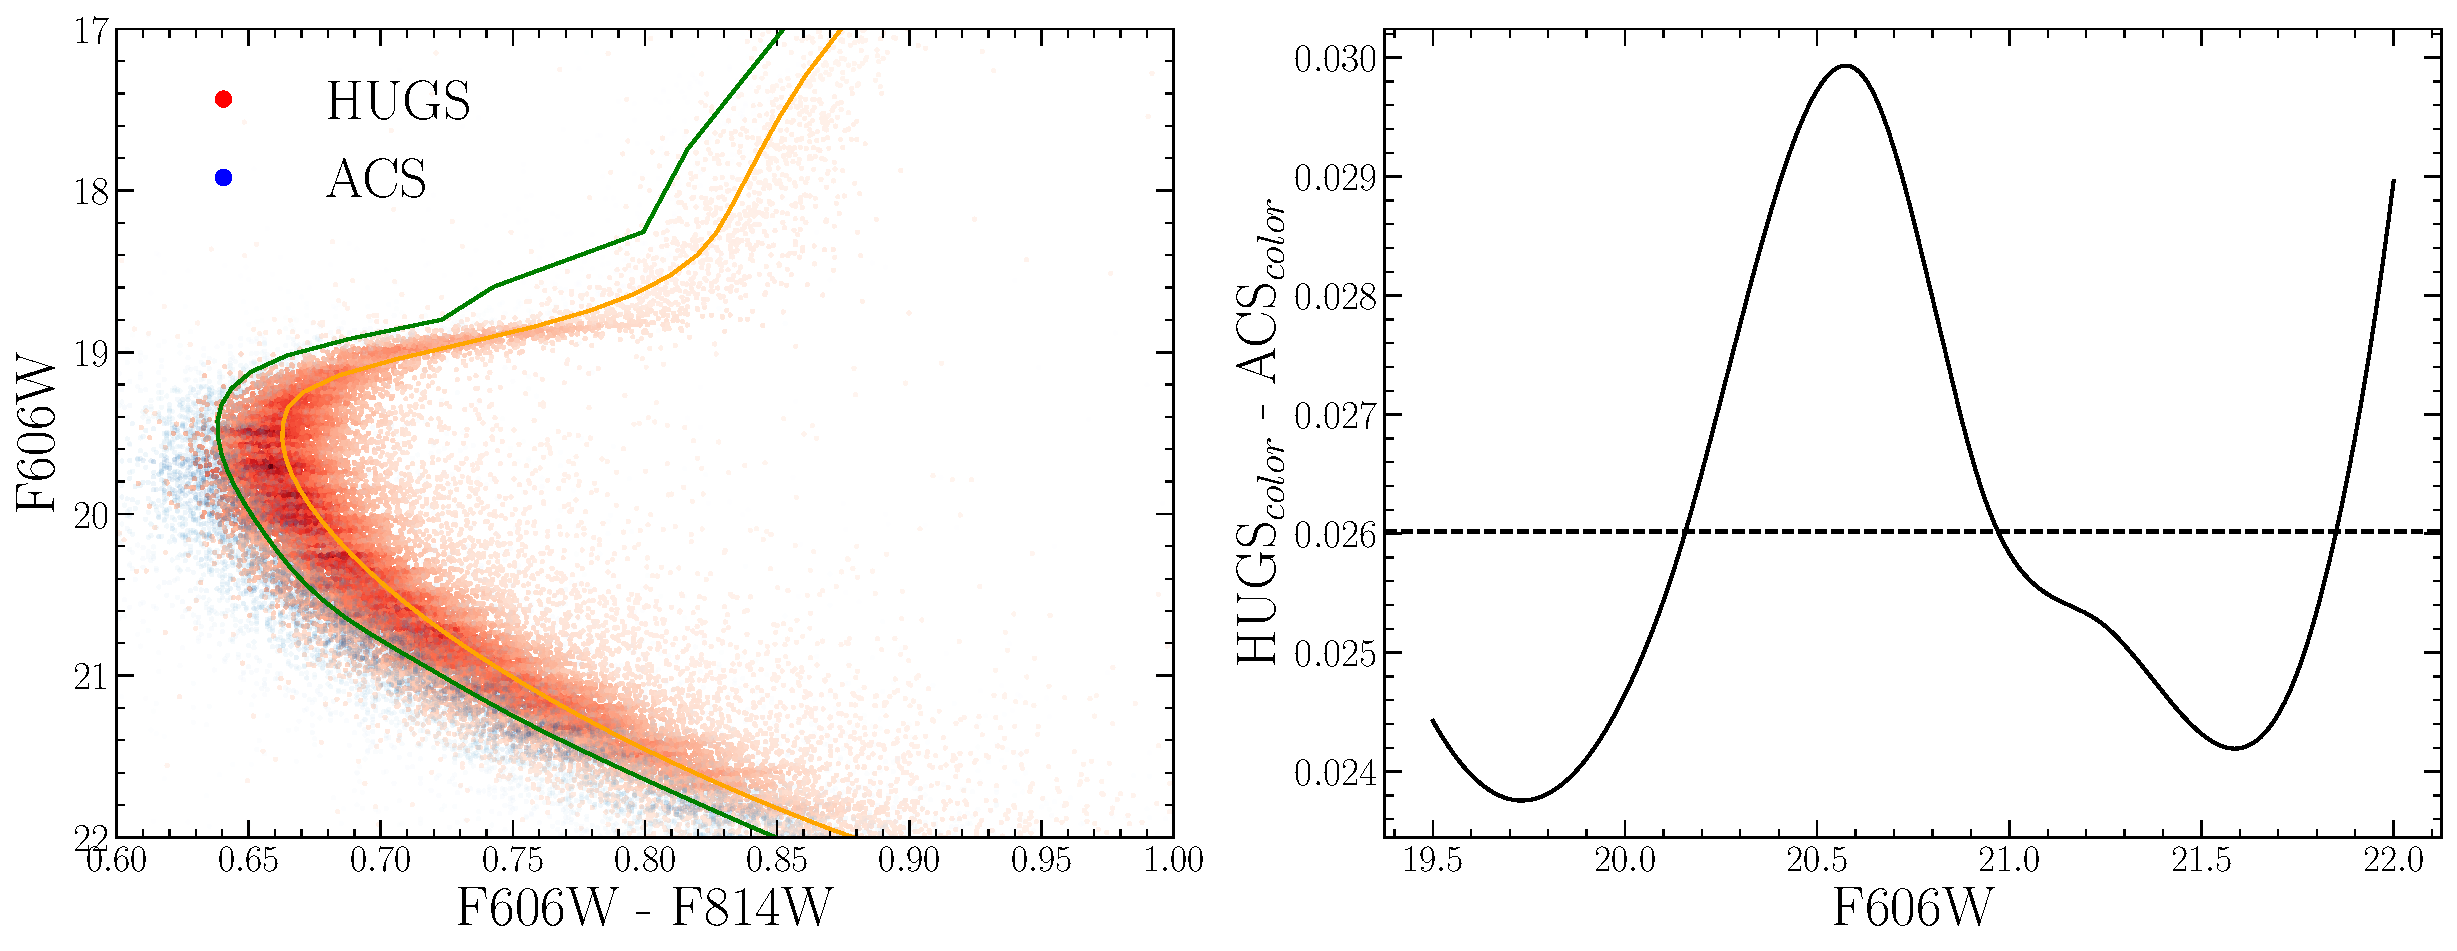
\includegraphics[width=0.90\textwidth]{figures/ngc2808/photometricOffset.pdf}
  \label{fig:offset}
  \caption{(left) CMD showing the photometric offset between the ACS and HUGS data for NGC 2808. CMDs have been randomly subsampled and colored by point density for clarity. (right) Mean difference between the color of the HUGS and ACS fiducual lines at the same magnitude. Note that the ACS data is systematically bluer than the HUGS data.}
\end{figure*}

The oberved photometric offset between ACS and HUGS reductions introduces a
systematic uncertainity when comparing parameters derived from isochrone fits
to ACS data vs those fit to HUGS data. Specifically, this offset introduces a
{\color{red}$\sim$AGE Gyr} uncertainity. Moreover, for two isochrone of the
same age, only seperated by helium mass fraction, a shift of the main sequence
turn off of is also expected. Figure \ref{fig:HeMO} shows this shift. Note a change in the helium mass fraction of a model by 0.03 results in an approximate 0.08 magnitude shift to the main sequence turn off location. This means that the mean 0.026 magnitude offset we find in between ACS and HUGS data corresponds to an additional approaximate 0.01 uncertainity in the derived helium mass fraction when comparing between these two datasets. 

\begin{figure}
  \centering
  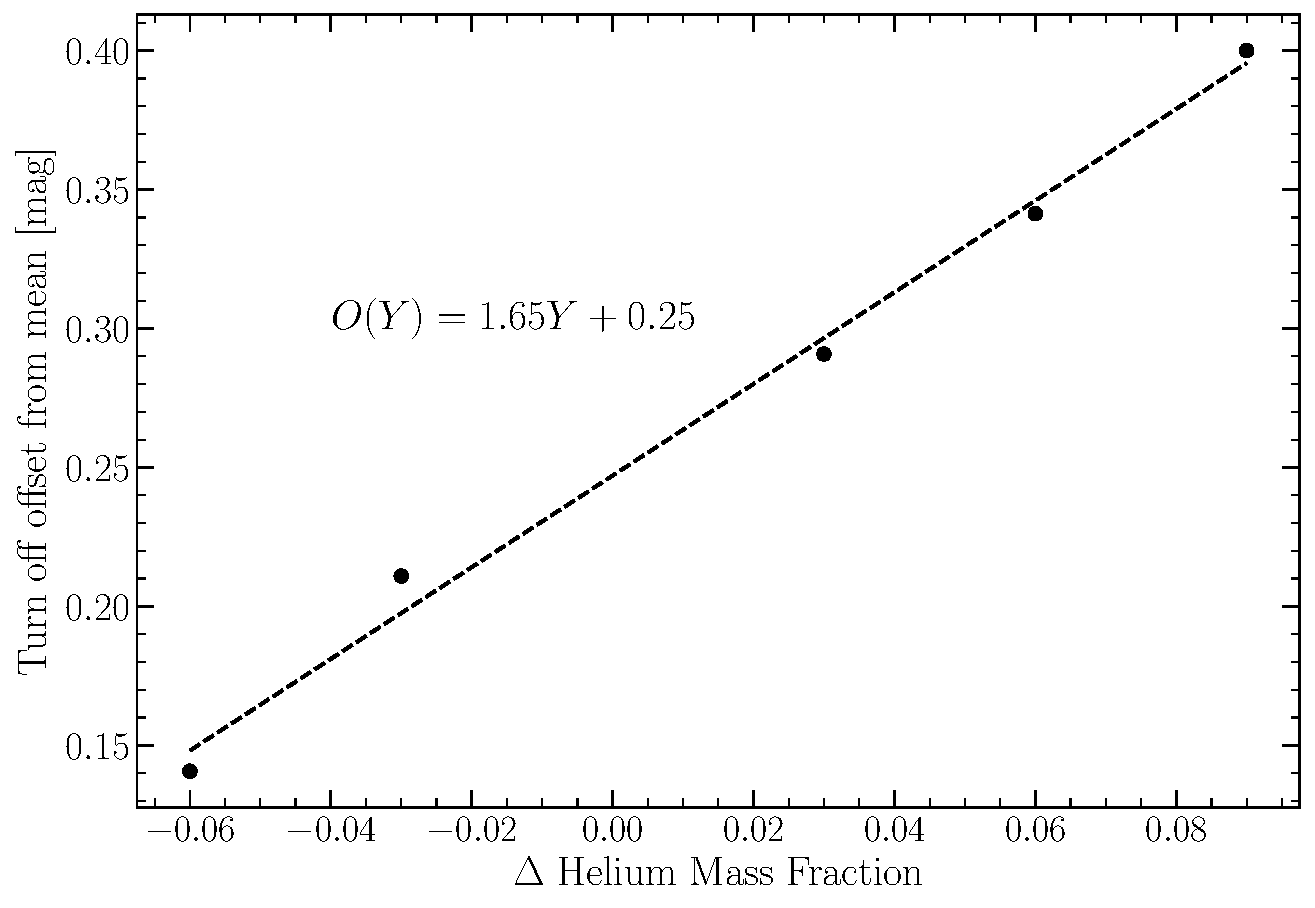
\includegraphics[width=0.45\textwidth]{figures/ngc2808/HeliumMeanOffset.pdf}
  \caption{Main sequence turn off magnitude offset from a guage helium mass fraction (Y=0.30 chosen). All main sequence turn off locations are measured at 12.3 Gyr {\color{blue} Should I make these contour surfaces for various ages?}}
  \label{fig:HeMO}
\end{figure}

\section{Correlation}\label{sec:results}
Using Ca II H\&K emission data from \citet{Boudreaux2022} and
\citet{Perdelwitz2021} (quantified using the $R_{HK}$ metric) we investigate
the correlation between the Jao Gap magnitude and stellar magnetic activity. We
are more statistically limited here than past authors have been due to
the requirement for high resolution spectroscopic data when measuring Calcium
emission; however, this is balanced by the apparent stronger correlation between
Calcium emission and the Jao gap when compared to H$\alpha$ emission. 

The merged dataset is presented in Figure \ref{fig:mergedData}. There is a
visual discontinuity just below the Jao Gap magnitude; however, this
manifests as an increase in the spread of the emission measurements rather than
a change in the mean value. In order to quantify the significance of this
discontinuity we measure the false alarm probability of the change in standard
deviation.

\begin{figure}
  \centering
  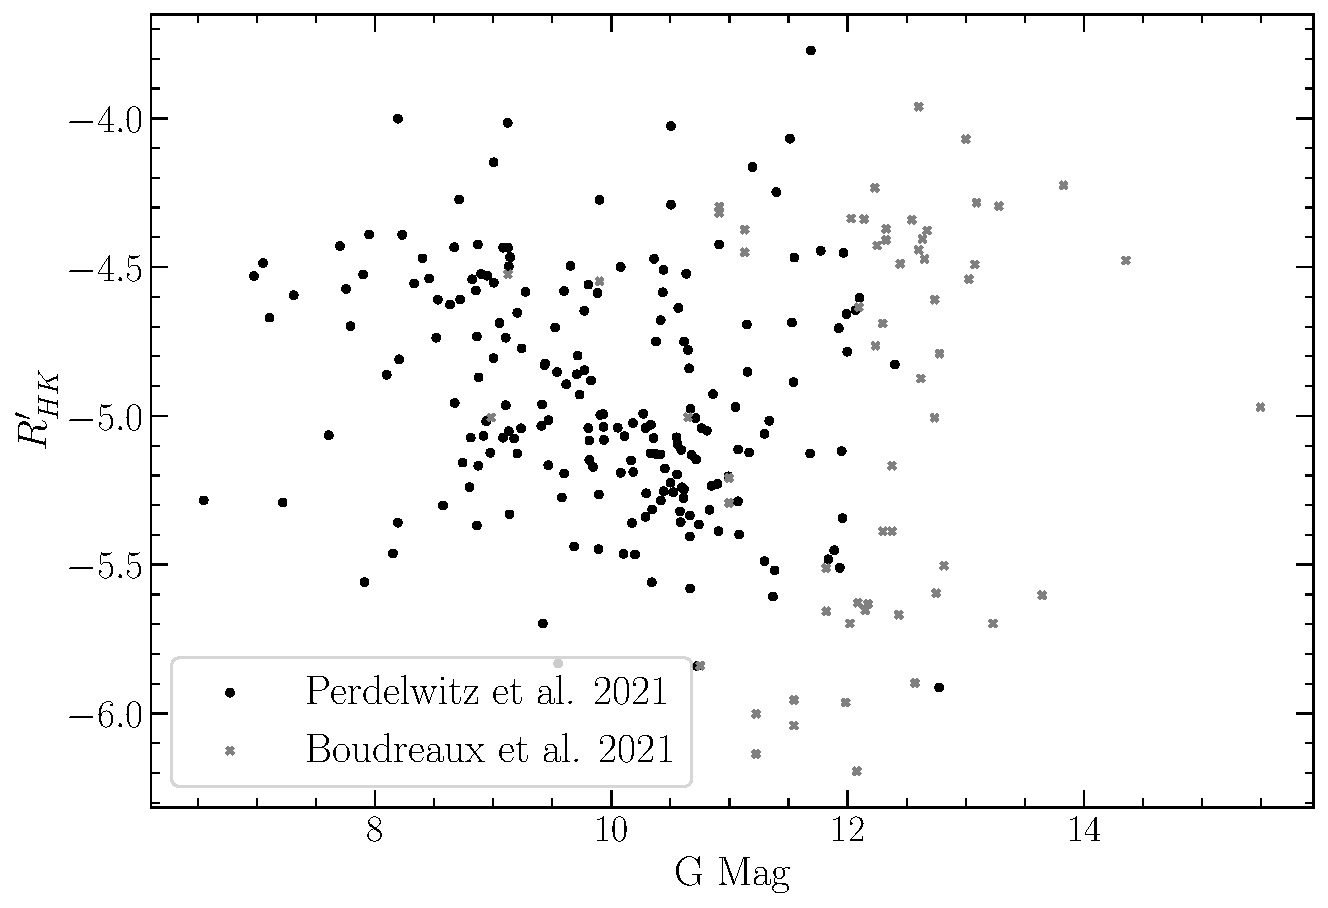
\includegraphics[width=0.45\textwidth]{figures/jaoMagActivity/Combined.pdf}
  \caption{Merged Dataset from \citet{Boudreaux2022, Perdelwitz2021}. Note the
  increase in the spread of $R'_{HK}$ around the Jao Gap Magnitude.}
  \label{fig:mergedData}
\end{figure}

First we split the merged dataset into bins with a width of 0.5 mag. In each bin we
measure the standard deviation about the mean of the data. The results of this
are shown in Figure \ref{fig:deviation}. In order to measure the false alarm
probability of this discontinuity we first resample the merged calcium
emission data based on the associated uncertainties for each datum as
presented in their respective publications. Then, for each of these ``resample
trials'' we measure the probability that a change in the standard deviation of
the size seen would happen purely due to noise. Results of this test are show in
in Figure \ref{fig:dist}. 

\begin{figure}
  \centering
  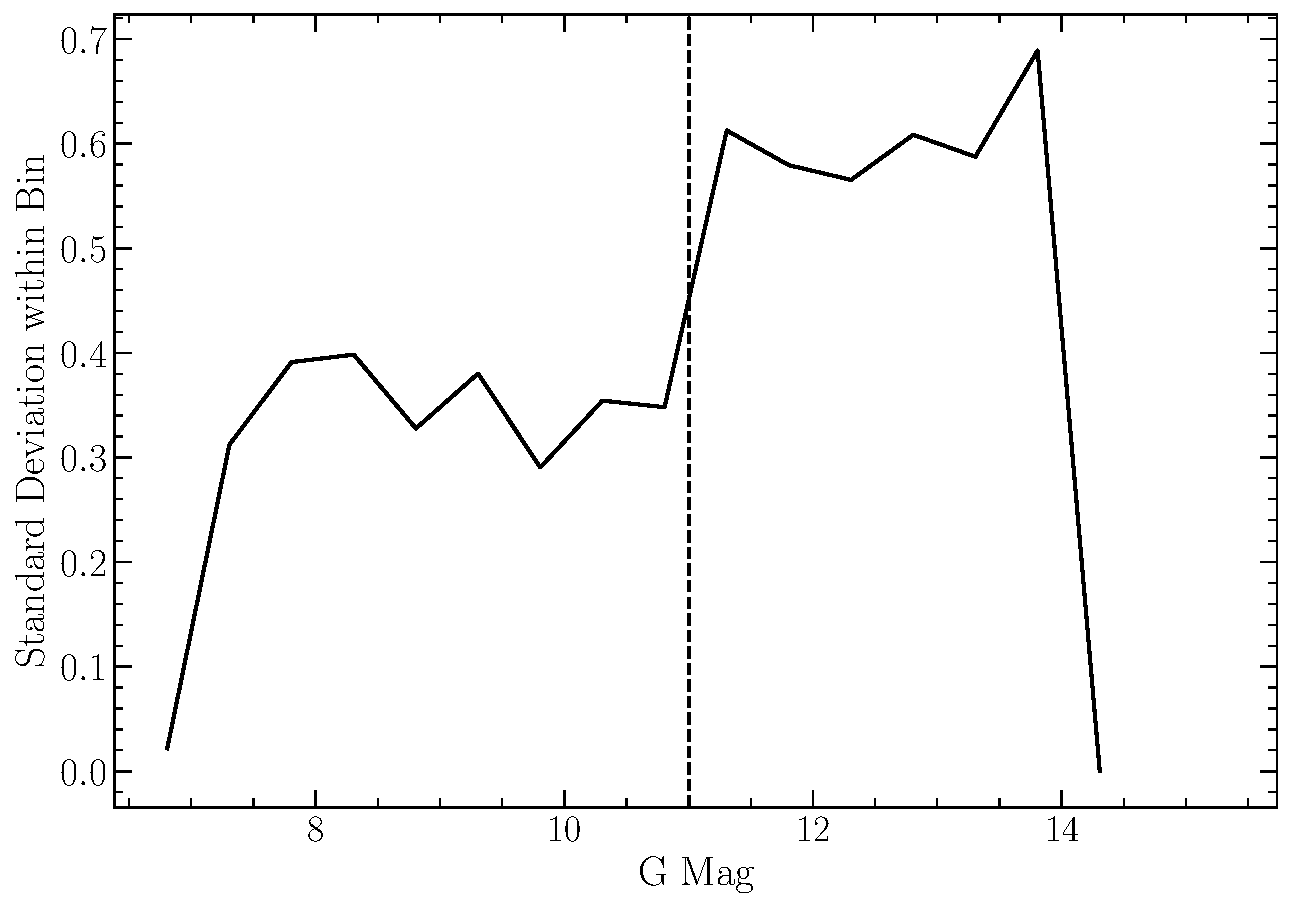
\includegraphics[width=0.45\textwidth]{figures/jaoMagActivity/Deviation.pdf}
  \caption{Standard deviation of Calcium emission data within each bin. Note
  the discontinuity near the Jao Gap Magnitude.}
  \label{fig:deviation}
\end{figure}

\begin{figure}
  \centering
  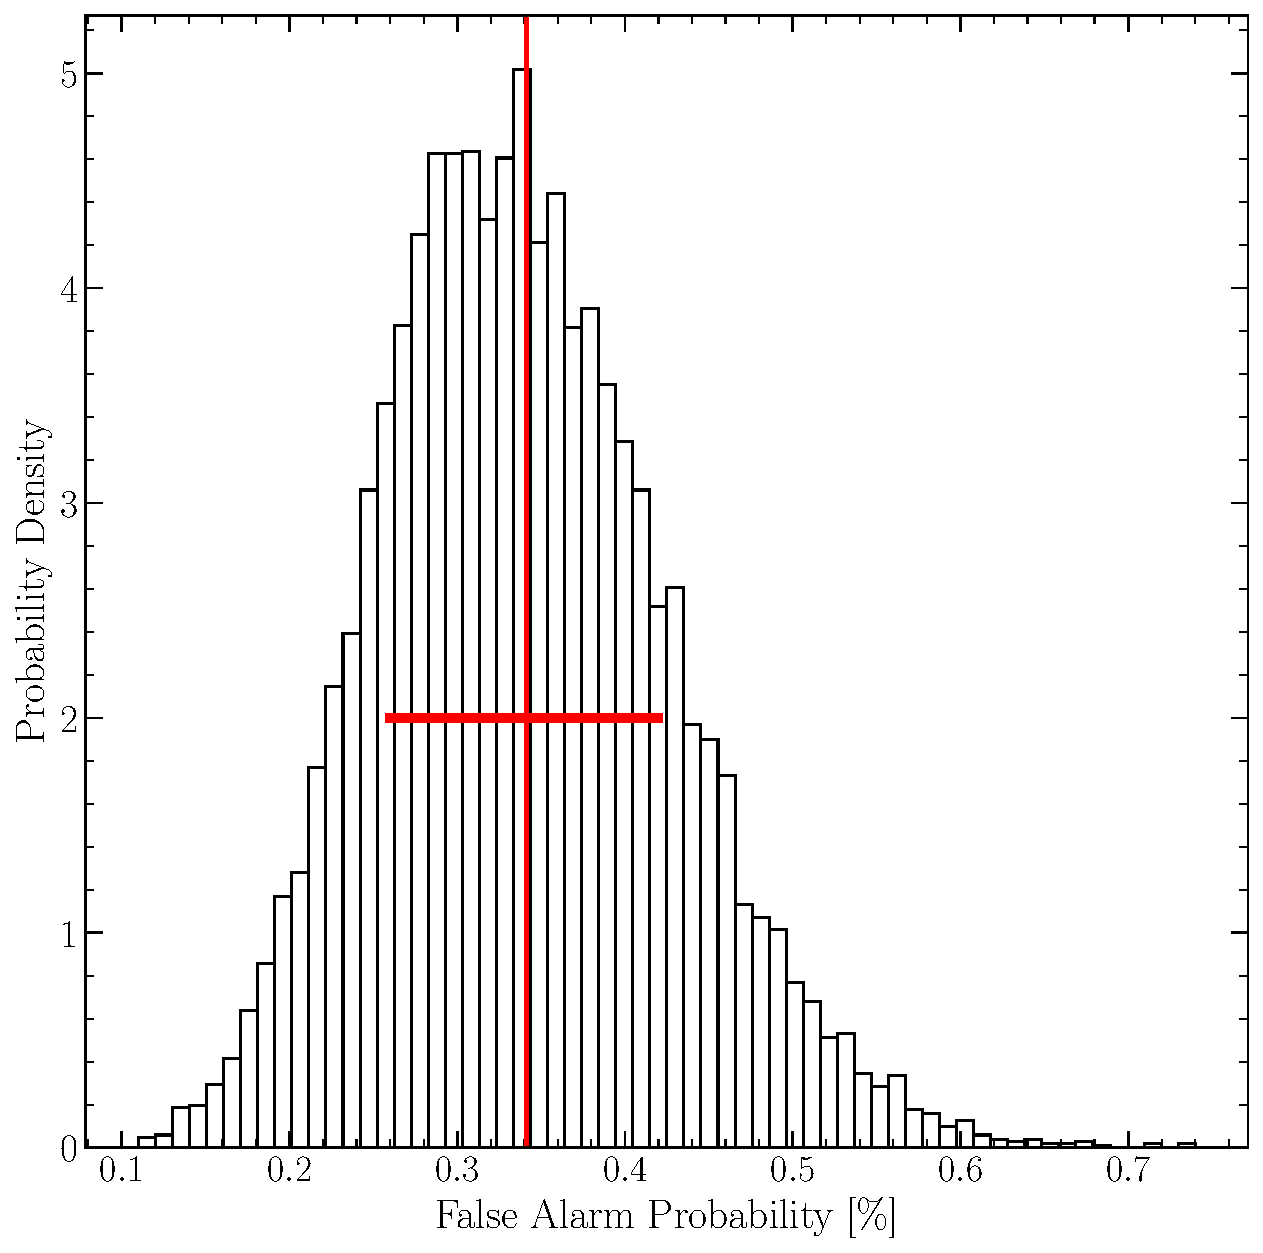
\includegraphics[width=0.45\textwidth]{figures/jaoMagActivity/fpDist.pdf}
  \caption{Probability distribution of the false alarm probability for the
  discontinuity seen in Figure \ref{fig:deviation}. The mean of this
  distribution is $0.341\%\pm^{0.08}_{0.08}$.}
  \label{fig:dist}
\end{figure}

This rapid increase star-to-star variability would only arise due purely to
noise $0.3\pm0.08$ percent of the time and is therefore likely either a true
effect or an alias of some sample bias. {\color{red} COME BACK TO HERE TO FLUSH
OUT SAMPLE BIAS SECTION.}

If the observed increase in variability is not due to a sample bias and rather
is a physically driven effect then there is an obvious similarity between these
findings and those of \citep{Jao2023}. Specifically we find a increase in
variability just below the magnitude of the gap. Moreover, this variability
increase is primarily driven by an increase in the number of low activity stars
(as opposed to an increase in the number of high activity stars). We can
further investigate the observed change in variability for only low activity
stars by filtering out those stars at or above the saturated threshold for
magnetic activity. \citet{Boudreaux2022} identify $\log(R'_{HK}) = -4.436$ as
the saturation threshold. We adopt this value and filter out all stars where
$\log(R'_{HK}) \geq -4.436$. Applying the same analysis to this reduced dataset
as was done to the full dataset we still find a discontinuity at the same
location (Figure \ref{fig:reduced}). This discontinuity is of a smaller
magnitude and consequently is more likely to be due purely to noise, with a
$7\pm0.2$ percent false alarm probability. This false alarm probability is
however only concerned with the first point after the jump in variability. If
we consider the false alarm probability of the entire high variability region
then the probability that the high variability region is due purely to noise
drops to $1.4\pm0.04$ percent.

\begin{figure}
  \centering
  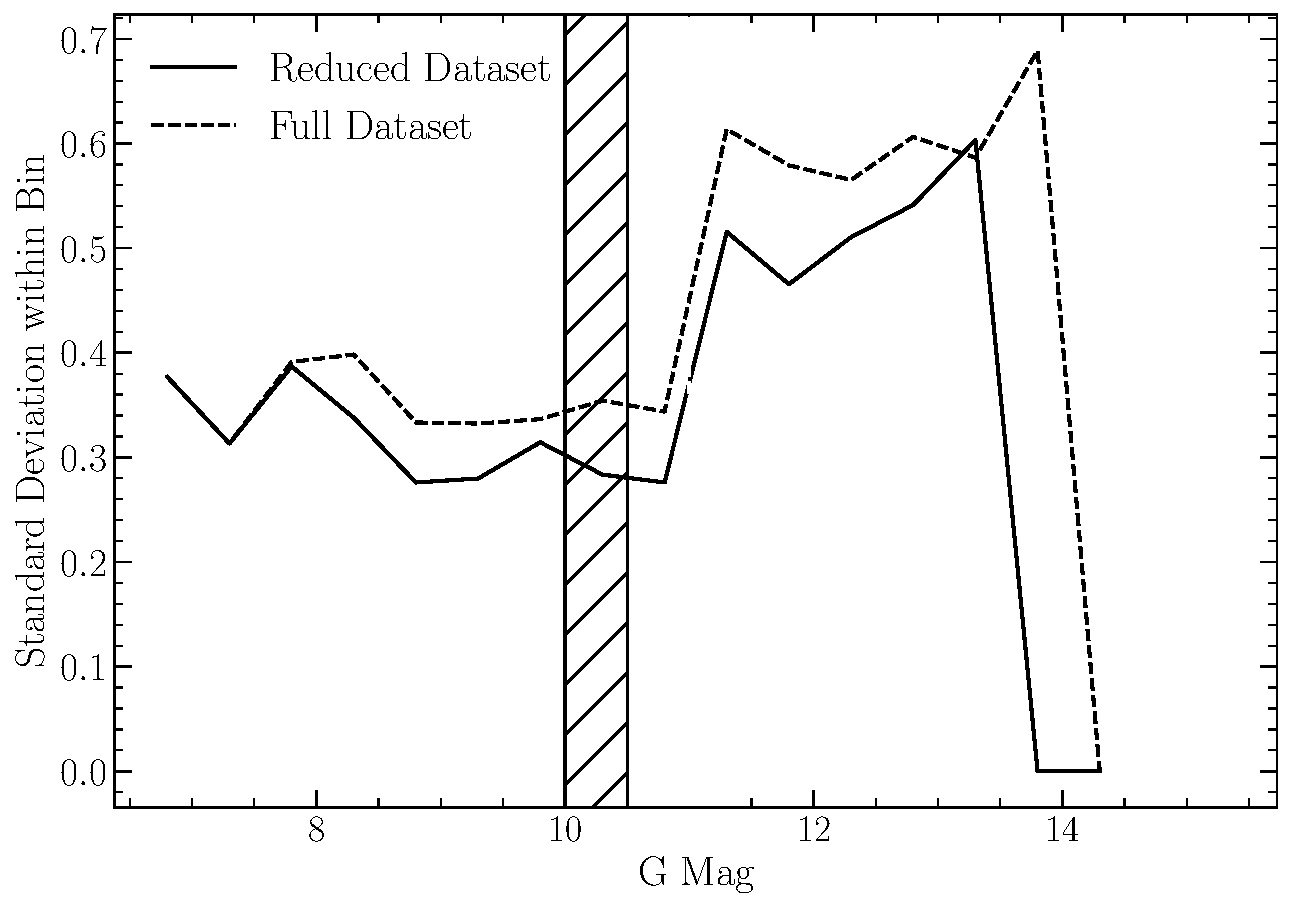
\includegraphics[width=0.45\textwidth]{figures/jaoMagActivity/ReducedDeviation.pdf}
  \caption{Spread in the magnetic activity metric for the merged sample with
  any stars $\log(R'_{HK}) > -4.436$ filtered out.}
  \label{fig:reduced}
\end{figure}

We observe a strong, likely statistically significant, discontinuity in the
star-to-star variability of Ca II K \& K emission just below the magnitude
of the Jao Gap. However, modeling is required to determine if this discontinuity
may be due to the same underlying physics.

While the observed increase in variability seen here does not seem to be
coincident with the Jao Gap --- instead appearing to be approximately 0.5 mag
fainter, in agreement with what is observed in \citet{Jao2023} --- a number of
complicating factors prevent us from falsifying that the these two features are
not coincident. \citeauthor{Jao2023} find, similar to the results presented
here, that the paucity of $H\alpha$ emission originates just below the gap.
Moreover, we use a 0.5 magnitude bin size when measuring the star-to-star
variability which injects error into the positioning of any feature in
magnitude space. We can quantify the degree of uncertainty the magnitude bin
choice injects by conducting Monte Carlo trials where bins are randomly shifted
redder or bluer. We conduct 10,000 trials where each trial involves sampling a
random shift to the bin start location from a normal distribution with a
standard deviation of 1 magnitude. For each trial we identify the discontinuity
location as the maximum value of the gradient of the standard deviation
(effectively this is just the derivative of \ref{fig:reduced}). Some trials
result in the maximal value lying at the 0th index of the magnitude array due
to edge effects, these trials are rejected (and account for 11\% of the
trials). The uncertainty in the identified magnitude of the discontinuity due
to the selected start point of the magnitude bins reveals a $1\sigma = \pm$0.32
magnitude uncertainty in the location of the discontinuity (Figure
\ref{fig:GapLocationMC}). Finally, all previous studies of the M dwarf gap
\citep{Jao2018, Feiden2022, Mansfield2021, Boudreaux2022, Jao2023} demonstrate
that the gap has a color dependency, shifting to fainter magnitudes as the
population reddens and consequently an exact magnitude range is ill-defined.
Therefore we cannot falsify the model that the discontinuity in star-to-star activity
variability is coincident with the Jao Gap magnitude.

\begin{figure}
  \centering
  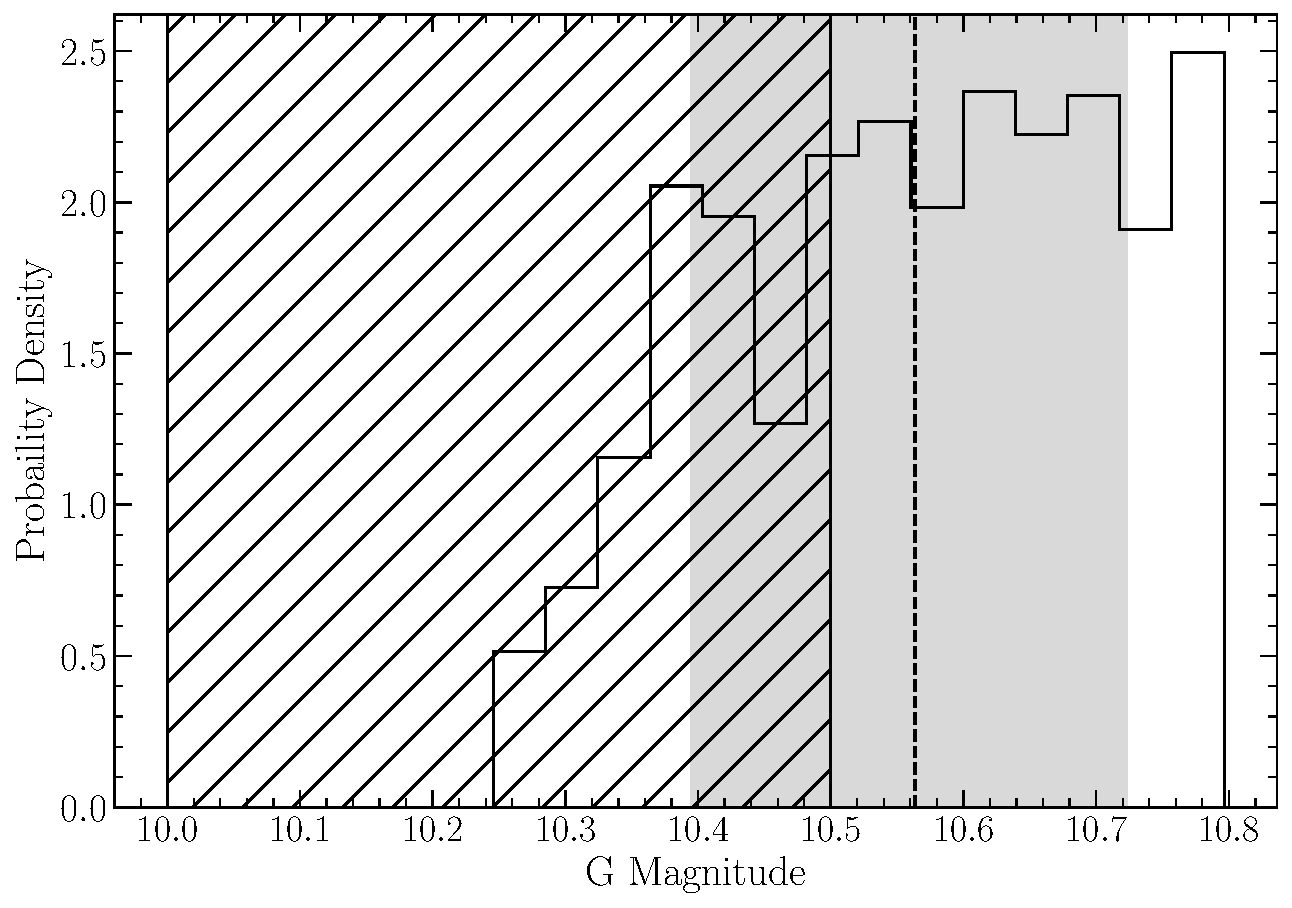
\includegraphics[width=0.45\textwidth]{figures/jaoMagActivity/GapLocationMC.pdf}
  \caption{Probability density distribution of discontinuity location as
  identified in the merged dataset. The dashed line represents the mean of the
  distribution while the shaded region runs from the 16th percentile to the
  84th percentile of the distribution. This distribution was built from 10,000
  independent samples where the discontinuity was identified as the highest
  value in the gradient of the standard deviation.}
  \label{fig:GapLocationMC}
\end{figure}

\subsection{Rotation}
Following the process described in \citet{023AJ....165..192G}, we first put the
dataset through \texttt{stella} \citep{FeinsteinFlare2020,FeinsteinStella2020},
a convolutional neural network that trains a multitude of models, given a
different initial seed, on TESS 2-min cadence. In this case, we also used an
ensemble of 100 models to optimize the gains. \texttt{stella} identifies flares
given a score of 0 to 1, here we use a score of 0.5 and above as flare
identification. Furthermore, we also bin the data from a 2-min to 10-min
cadence using \texttt{lightkurve}'s binning function
\citep{LightkurveCollaborationLightkurve2018,GeertBarentsenKeplerGO2020}. Not
only does this help further reduce any flaring-contribution that might have
been missed by \texttt{stella}\footnote{This is relevant for flares that are
misshapen at the start or break in the dataset due to missing either the
ingress or egress.}, but it also optimizes computational efficiency.
Subsequently, we calculate residuals by subtracting the model from the data,
retaining data with residuals smaller than 4 times the root-mean-square.

As M dwarfs often exhibit non-sinusoidal and quasi-periodic rotational
variability, we employ Gaussian processes for modeling based on
\citet{AngusInferring2018} for the subset of M Dwarfs with no fiducial periods.
The \texttt{starspot} \ package is adapted for light curve analysis
\citep{AngusRuthAngus2021,https://doi.org/10.5281/zenodo.7697238} and
accessible at (HAVEN'T DONE IT YET-AYLIN). Our Gaussian process kernel function
incorporates two stochastically-driven simple harmonic oscillators,
representing primary ($P_\textrm{rot}$) and secondary ($P_\textrm{rot}/2$)
rotation modes. First, we implement the Lomb-Scargle periodogram within
\texttt{starpot} to initially estimate the period. After which, we create a
maximum a posteriori (MAP) fit using \texttt{starspot} to generate a model for
stellar rotation. To obtain the posterior of the stellar rotation model, we use
Markov Chain Monte Carlo (MCMC) sampling using the \texttt{pymc3} package
\citep{SalvatierProbabilistic2016} within our adapted \texttt{starspot}
version. 

ANALYSIS PART YET TO BE DETERMINED.

\subsection{Limitations}
There are two primary limitation of our dataset. First, we only have
{\color{red}232 stars} in our dataset limiting the statistical power of our
analysis. This is primarily due to the relative difficulty of obtaining Ca II
H\&K measurements compared to obtaining $H\alpha$ measurements. Reliable
measurements require both high spectral resolutions ({\color{red} R $\sim$
XXXXXX}) and a comparatively blue wavelength range \footnote{wrt. too what many
spectrographs cover. There is no unified resource listing currently
commissioned spectrographs; however, it is somewhat hard to source glass which
transmits well at H\&K wavelengths limiting the lower wavelength of most
spectrographs.}.

Additionally, the sample we do have does not extend to as low mass as would be
ideal. This presents a degeneracy between two potential causes for the observed
increased star-to-star variability. One option, as presented above and
elaborated on in the following section, is that this is due to kissing
instabilities. However, another possibility is that this increased variability
is intrinsic to the magnetic fields of fully convective stars. There is limited
discussion in the literature of the latter effect; however, \citet{Shulyak2019}
present estimated magnetic field strengths for 47 M dwarfs, spanning a larger
area around the convective transition region and their dataset does not
indicate a inherently increased variability for fully convective stars
({\color{red} fully confirm this, not just visually}).

\section{Conclusion}\label{sec:conclusion}
It is, at this point, well established that the Jao Gap may provide a unique view of the interiors of stars for which other probes, such as seismology, fail. However, it has only recently become clear that the Gap may lend insight into not just structural changes within a star but also into the magnetic environment of the star.
\citet{Jao2023} presented evidence that the physics driving the Gap might additionally result in a paucity of H$\alpha$ emission. These authors propose potential physical mechanisms which could explain this paucity, including the core of the star acting as an angular momentum sink during mixing events.

Here we have expanded upon this work by probing the degree and variability of
Calcium II H\&K emission around the Jao Gap. We lack the same statistical
power of \citeauthor{Jao2023}'s sample; however, by focusing on the
star-to-star variability within magnitude bins we are able to retain
statistical power. We find that there is an anomalous increase in variability
at a G magnitude of $\sim 11$. This is only slightly below the observed mean gap magnitude.

Additionally, we propose a simple model to explain this variability. Making the
assumption that the periodic convective mixing events will have some small but
random effect on the overall magnetic field strength we are able to
qualitatively reproduce the increase activity spread in a synthetic population
of stars. 




\chapter{Gap Sensitivity to Opacity Source}
\section{Introduction}\label{sec:Intro}
Globular clusters (GCs) are among the oldest observable objects in the universe
\citep{Pen11}. They are characterized by high densities with typical half-light
radii of $\le$10 pc \citep{Vanderburg2010}, and typical masses ranging from
$10^{4}$--$10^{5}$ M$_{\odot}$ \citep{Bro06} --- though some GCs are
significantly larger than these typical values \citep[e.g. $\omega$ Cen,
][]{Richer1991}. GCs provide a unique way to probe stellar evolution
\citep{Bau03}, galaxy formation models \citep{Boy18,Kra05}, and dark matter
halo structure \citep{Hud18}.

The traditional view of Globular Clusters was that they consisted of a single
stellar population (SSP, in some publications this is referred to as a Simple
Stellar Population). This view was supported by spectroscopically uniform heavy
element abundances \citep{Carretta2010, Bastian2018} across most clusters (M54
and $\omega$Cen are notable exceptions, see \citet{Marino2015} for further
details), and the lack of evidence for multiple stellar populations (MPs) in
past color-magnitude diagrams of GCs \citep[i.e.][]{Sandage1953, Alcaino1975}.
However, over the last 40 years non-trivial star-to-star light-element
abundance variations have been observed \citep[i.e.][]{Smith1987} and, in the
last two decades, it has been definitively shown that most if not all Milky Way
GCs have MPs \citep{Gratton2004, Gratton2012, Piotto2015}. The lack of
photometric evidence for MPs prior to the 2000, can be attributed to the more
narrow color bands available, until very recently, to ground based photometric
surveys \citep{Milone2017}.

The prevalence of multiple populations in GCs is so distinct that the proposed
definitions for what constitutes a globular cluster now often center the
existence of MPs \citep[e.g.][]{Carretta2010}. Whereas, people have have often
tried to categorized objects as GCs through relations between half-light
radius, density, and surface brightness profile, in fact many objects which are
generally thought of as GCs don't cleanly fit into these cuts
\citep{Peebles1968, Brown1991, Brown1995, Bekki2002}. Consequently,
\citet{Carretta2010} proposed a definition of GC based on observed chemical
inhomogeneities in their stellar populations. The modern understanding of GCs
then is not simply one of a dense cluster of stars that may have chemical
inhomogeneities and multiple populations; rather, it is one where those
chemical inhomogeneities and multiple populations themselves are the defining
element of a GC.

All Milky Way globular clusters studied in detail show populations enriched in
He, N, and Na while also being deplete in O and C
\citep{Piotto2015,Bastian2018}. {\bf Further, studies of Magellenic Cloud
massive clusters have shown that these light element abundance variations exist
in clusters as young as $\sim 2$ Gyr but not in younger clusters
\citep{Martocchia2019} while there is also evidence of nitrogen variability in
the $\sim 1.5$ Gyr old cluster NGC 1783 \citep{Cadelano2022}}.  These light
element abundance patterns also are not strongly correlated with variations in
heavy element abundance, resulting in spectroscopically uniform Fe abundances
between populations \citep[{\bf though recent work indicates that there may be
[Fe/H] variations within the first population, e.g.}][]{Legnardi2022,
Lardo2022} . Further, high-resolution spectral studies reveal anti-correlations
between N-C abundances, Na-O abundances, and potentially Al-Mg
\citep{Sneden1992, Gratton2012}. Typical stellar fusion reactions can deplete
core oxygen; however, the observed abundances of Na, Al, and Mg cannot be
explained by the CNO cycle \citep{Prantzos2007}. Consequently, globular cluster
populations must be formed by some novel means.

Formation channels for these multiple populations remain a point of debate
among astronomers. Most proposed formation channels consist of some older,
more massive, population of stars polluting the pristine cluster media before a
second population forms, now enriched in heavier elements which they themselves could
not have generated \citep[for a detailed review see ][]{Gratton2012}. The four
primary candidates for these polluters are asymptotic giant branch stars
\citep[AGBs,][]{Ventura2001,DErcole2010}, fast rotating massive stars
\citep[FRMSs,][]{Decressin2007}, super massive stars
\citep[SMSs,][]{Denissenkov2014}, and massive interacting binaries
\citep[MIBs,][]{deMink2009, Bastian2018}. 

Hot hydrogen burning (i.e. proton capture), material transport to the surface, and
material ejection into the intra-cluster media are features of each of these
models and consequently they can all be made to {\it qualitatively} agree with
the observed elemental abundances. However, none of the standard models can
currently account for all specific abundances \citep{Gratton2012}. AGB and FRMS
models are the most promising; however, both models have difficulty reproducing
severe O depletion \citep{Ventura2009,Decressin2007}. Moreover, AGB and FRMS
models require significant mass loss ($\sim 90\%$) between cluster formation
and the current epoch --- implying that a significant fraction of halo stars
formed in GCs \citep{Renzini2008,DErcole2008,Bastian2015}.

In addition to the light-element anti-correlations observed, it is also known
that second populations are significantly enhanced in Helium
\citep{Piotto2007, Piotto2015, Latour2019}. Depending on the cluster, helium
mass fractions as high as $Y=0.4$ have been inferred \citep[e.g][]{Milone2015}.
However, due to both the relatively high and tight temperature range of partial
ionization for He and the efficiency of gravitational settling in core helium
burning stars, the initial He abundance of globular cluster stars cannot be
observed; consequently, the evidence for enhanced He in GCs originates from
comparison of theoretical stellar isochrones to the observed
color-magnitude-diagrams of globular clusters. Therefore, a careful handling of
chemistry is essential when modeling with the aim of discriminating between
MPs; yet, only a very limited number of GCs have been studied with
chemically self-consistent (structure and atmosphere) isochrones
\citep[e.g.][NGC 6752]{Dotter2015}. 

NGC 2808 is the prototype globular cluster to host Multiple Populations.
Various studies since 2007 have identified that it may host anywhere from 2-5
stellar populations. These populations have been identified both
spectroscopically \citep[i.e.][]{Carretta2004, Carretta2006, Carretta2010,
Gratton2011, Carretta2015, Hong2021} and photometrically
\citep[i.e.][]{Piotto2007, Piotto2015, Milone2015, Milone2017, Pasquato2019}.
Note that recent work \citep{Valle2022} calls into question the statistical
significance of the detections of more than 2 populations in the spectroscopic
data. Here we present new, chemically self-consistent modeling of the
photometry of the two extreme populations of NGC 2808 identified by
\citet{Milone2015}, populations A and E. {\bf We do not consider populations B,
C, or D identified in \citet{Milone2015} as the purpose of this work is to
identify if chemically self-consistent modelling results in a statisically
signifigant deviation in the infered helium abundance when compared to non
chemically self-consistent models. Use of the two populations in the NGC 2808
with the highest identified difference between their helium populations is
sufficent for to answer this question.}  We use archival photometry from the
Hubble UV Globular Cluster Survey (HUGS) \citep{Piotto2015, Milone2017} in the
F275W and F814W passbands to characterize multiple populations in NGC 2808
\citep{Milone2015, Milone2015b} (This data is avalible at MAST: \href{https://archive.stsci.edu/doi/resolve/resolve.html?doi=10.17909/T9810F}{10.17909/T9810F}). Additionally, we present a
likelihood analysis of the photometric data of NGC 2808 to determine the number
of populations present in the cluster.



\section{The Underlying Physics of the Gap}\label{sec:JaoGap}
A theoretical explanation for the Jao Gap (Figure \ref{fig:JaoGap}) comes from
\citet{van2012}, who propose that in a star directly above the transition mass,
due to asymmetric production and destruction of $^{3}$He during the
proton-proton I chain (ppI), periodic luminosity variations can be induced.
This process is known as convective-kissing instability. Very shortly after the
zero-age main sequence such a star will briefly develop a radiative core;
however, as the core temperature exceeds $7\times 10^{6}$ K, enough energy will
be produced by the ppI chain that the core once again becomes convective. At
this point the star exists with both a convective core and envelope, in
addition to a thin, radiative layer separating the two. Subsequently,
asymmetries in ppI affect the evolution of the star's convective core.

While kissing instability has been the most widely adopted model to
explain the existence of the Jao Gap, slightly different mechanisms have also
been proposed. \citet{MacDonald2018} make use of a fully implicit stellar
evolution suite which treats convective mixing as a diffusive property.
\citeauthor{MacDonald2018} treat convective mixing this way in order to account
for a core deuterium concentration gradient proposed by \citet{Baraffe1997}.
Under this treatment the instability results only in a single mixing event ---
as opposed to periodic mixing events. Single mixing events may be more in line with
observations (see section \ref{sec:results} for more details on how periodic
mixing can effect a synthetic population) where there is only well documented
evidence of a single gap. However, recent work by \citet{Jao2021} which
identify an second under density of stars below the canonical gap, does leave
the door open for the periodic mixing events.

\begin{figure}
	\centering
	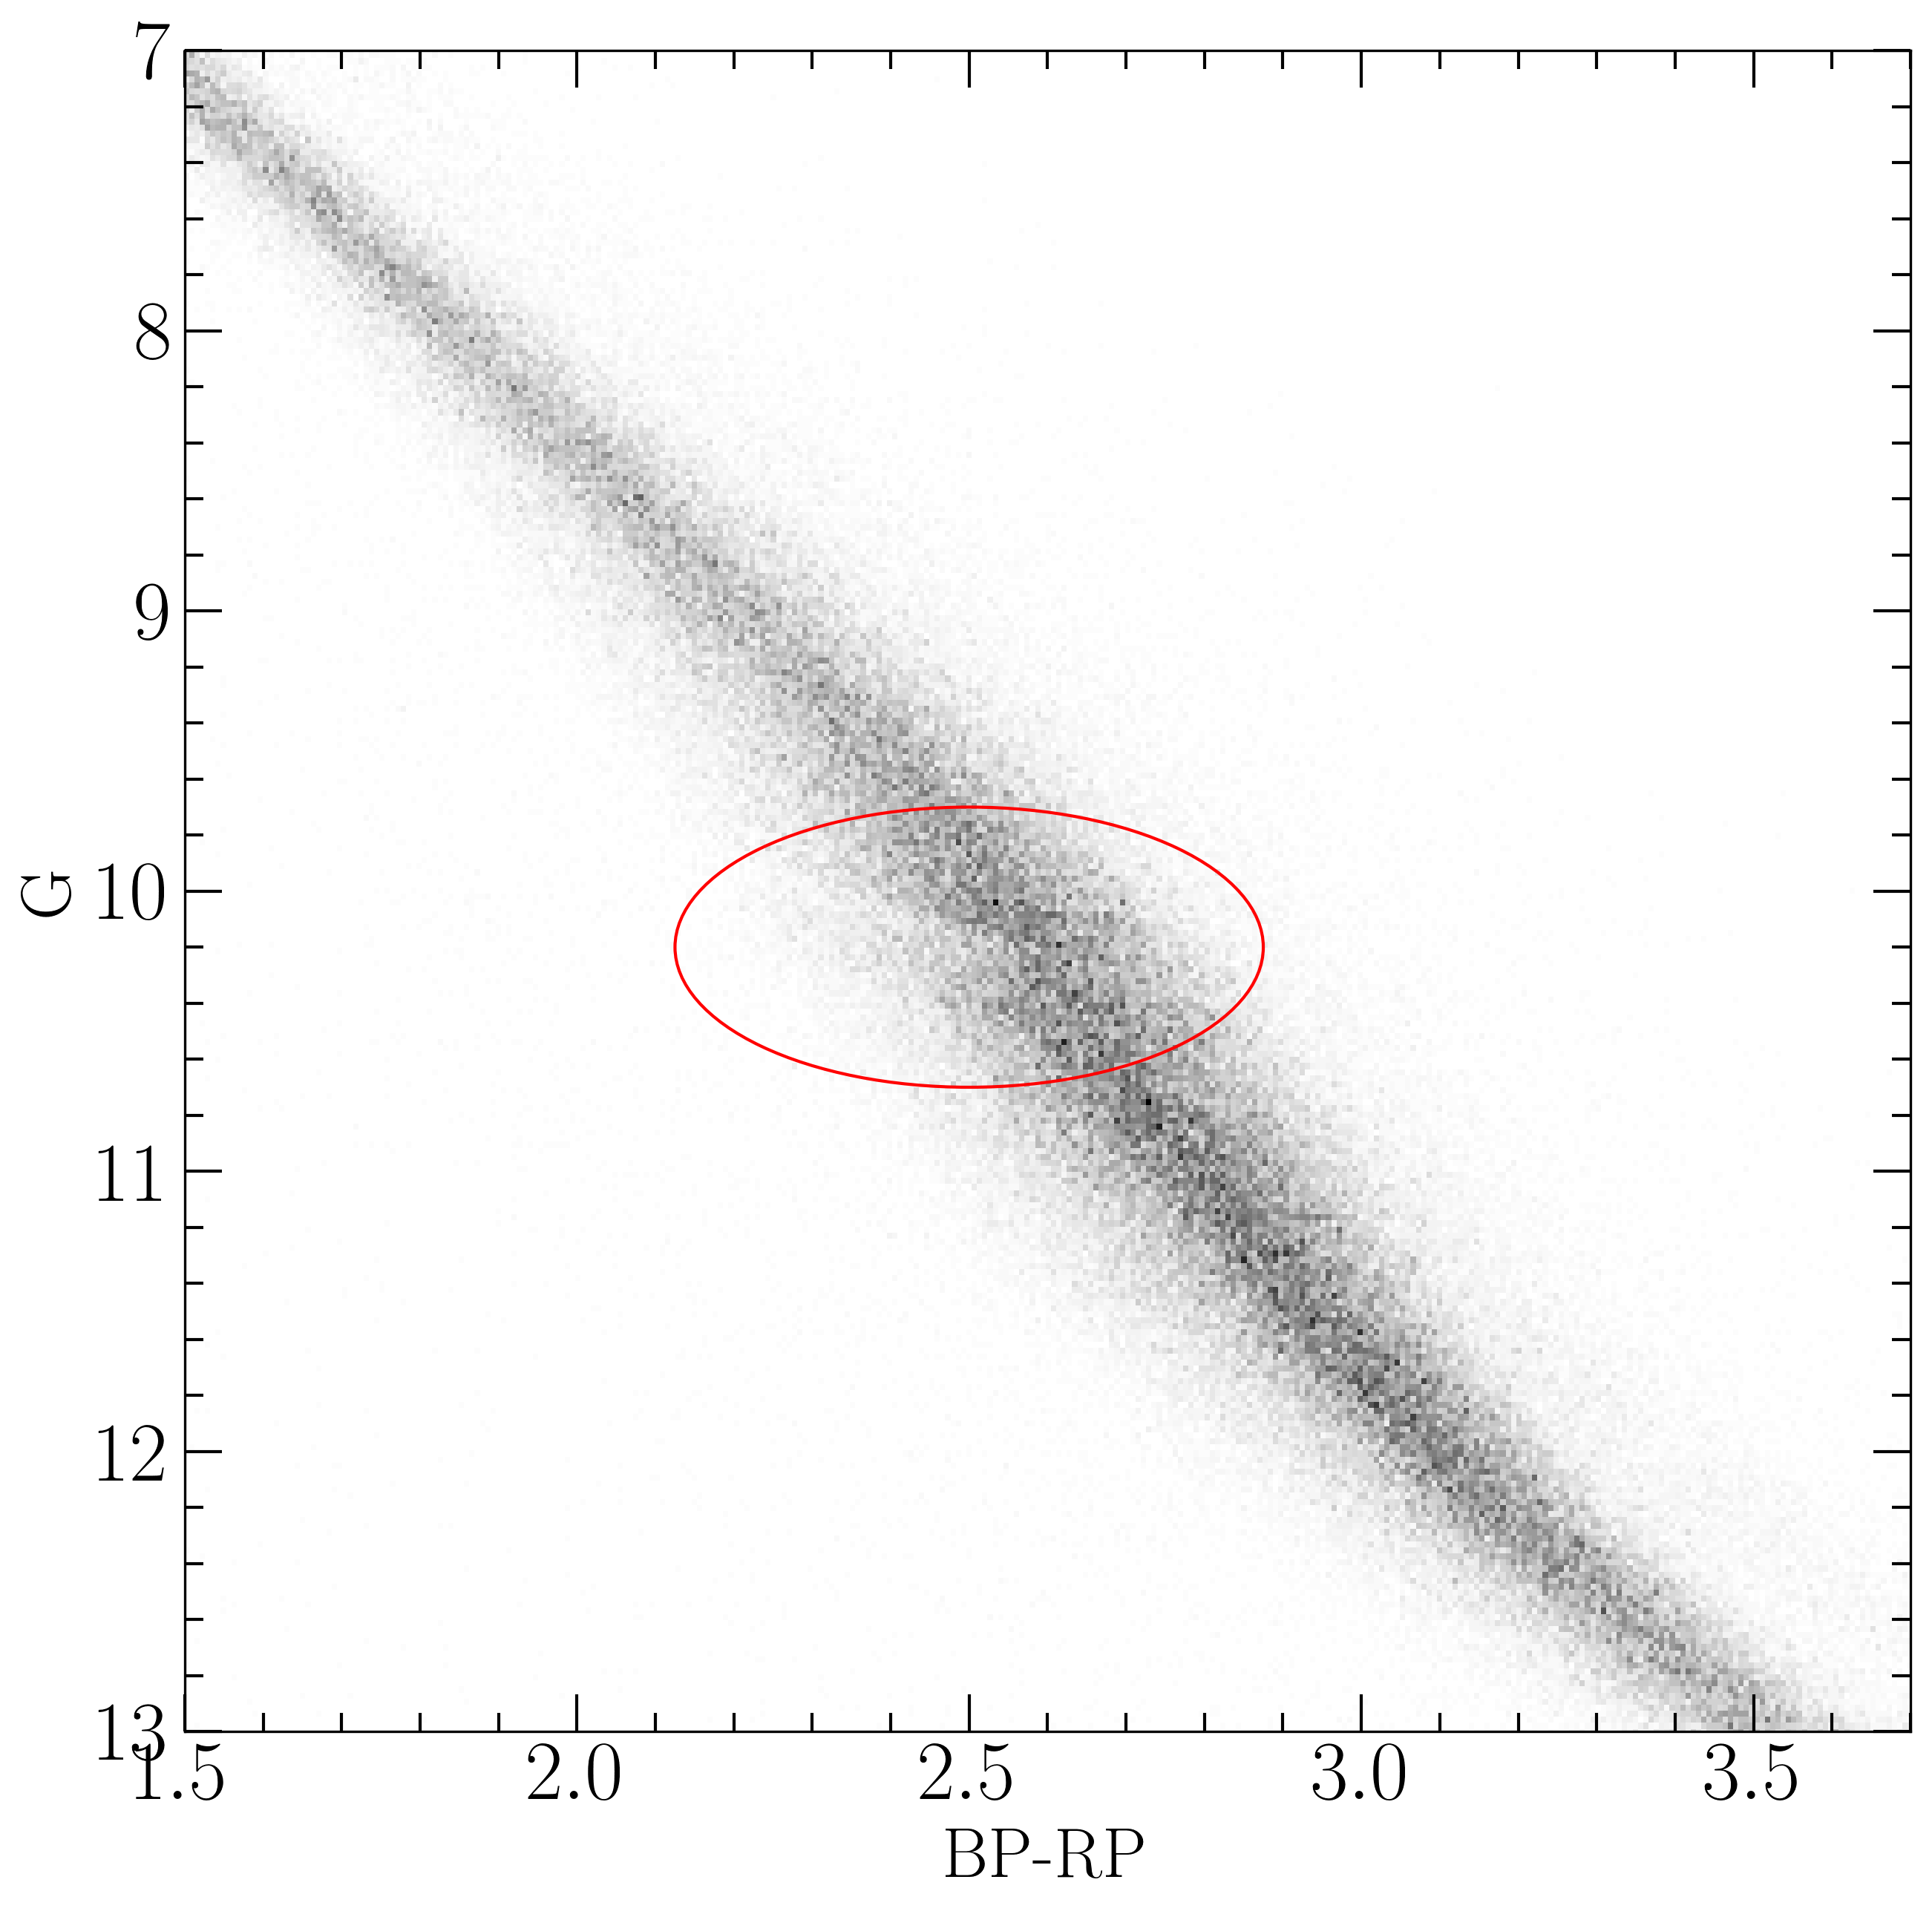
\includegraphics[width=0.85\textwidth]{figures/jaoOpacity/JaoGapEDR3.png}
	\caption{The Jao Gap (circled) seen in the Gaia Catalogue of Nearby Stars \citep{GaiaCollaboration2021}.}
	\label{fig:JaoGap}
\end{figure}

The proton-proton I chain constitutes three reactions 
\begin{enumerate} 
	\item $p + p \longrightarrow d + e^{+} + \nu_{e}$
	\item $p + d \longrightarrow \ ^{3}\text{He} + \gamma$
	\item $^{3}\text{He} + ^{3}\text{He} \longrightarrow \ ^{3}\text{He} + 2p$ 
\end{enumerate} 
Initially, reaction 3 of ppI consumes $^{3}$He at a slower rate than it is
produced by reaction 2 and as a result, the core $^{3}$He abundance and
consequently the rate of reaction 3, increases with time. The core convective
zone expands as more of the star becomes unstable to convection. This expansion
continues until the core connects with the convective envelope. At this point
convective mixing can transport material throughout the entire star and the
high concentration of $^{3}$He rapidly diffuses outward, away from the core,
decreasing energy generation as reaction 3 slows down. Ultimately, this leads
to the convective region around the core pulling back away from the convective
envelope, leaving in place the radiative transition zone, at which point
$^{3}$He concentrations grow in the core until it once again expands to meet
the envelope.  These periodic mixing events will continue until $^{3}$He
concentrations throughout the star reach an equilibrium ultimately resulting in
a fully convective star. Figure \ref{fig:Kippenhan1} traces the evolution of a
characteristic star within the Jao Gap's mass range.

\begin{figure*}
	\centering
	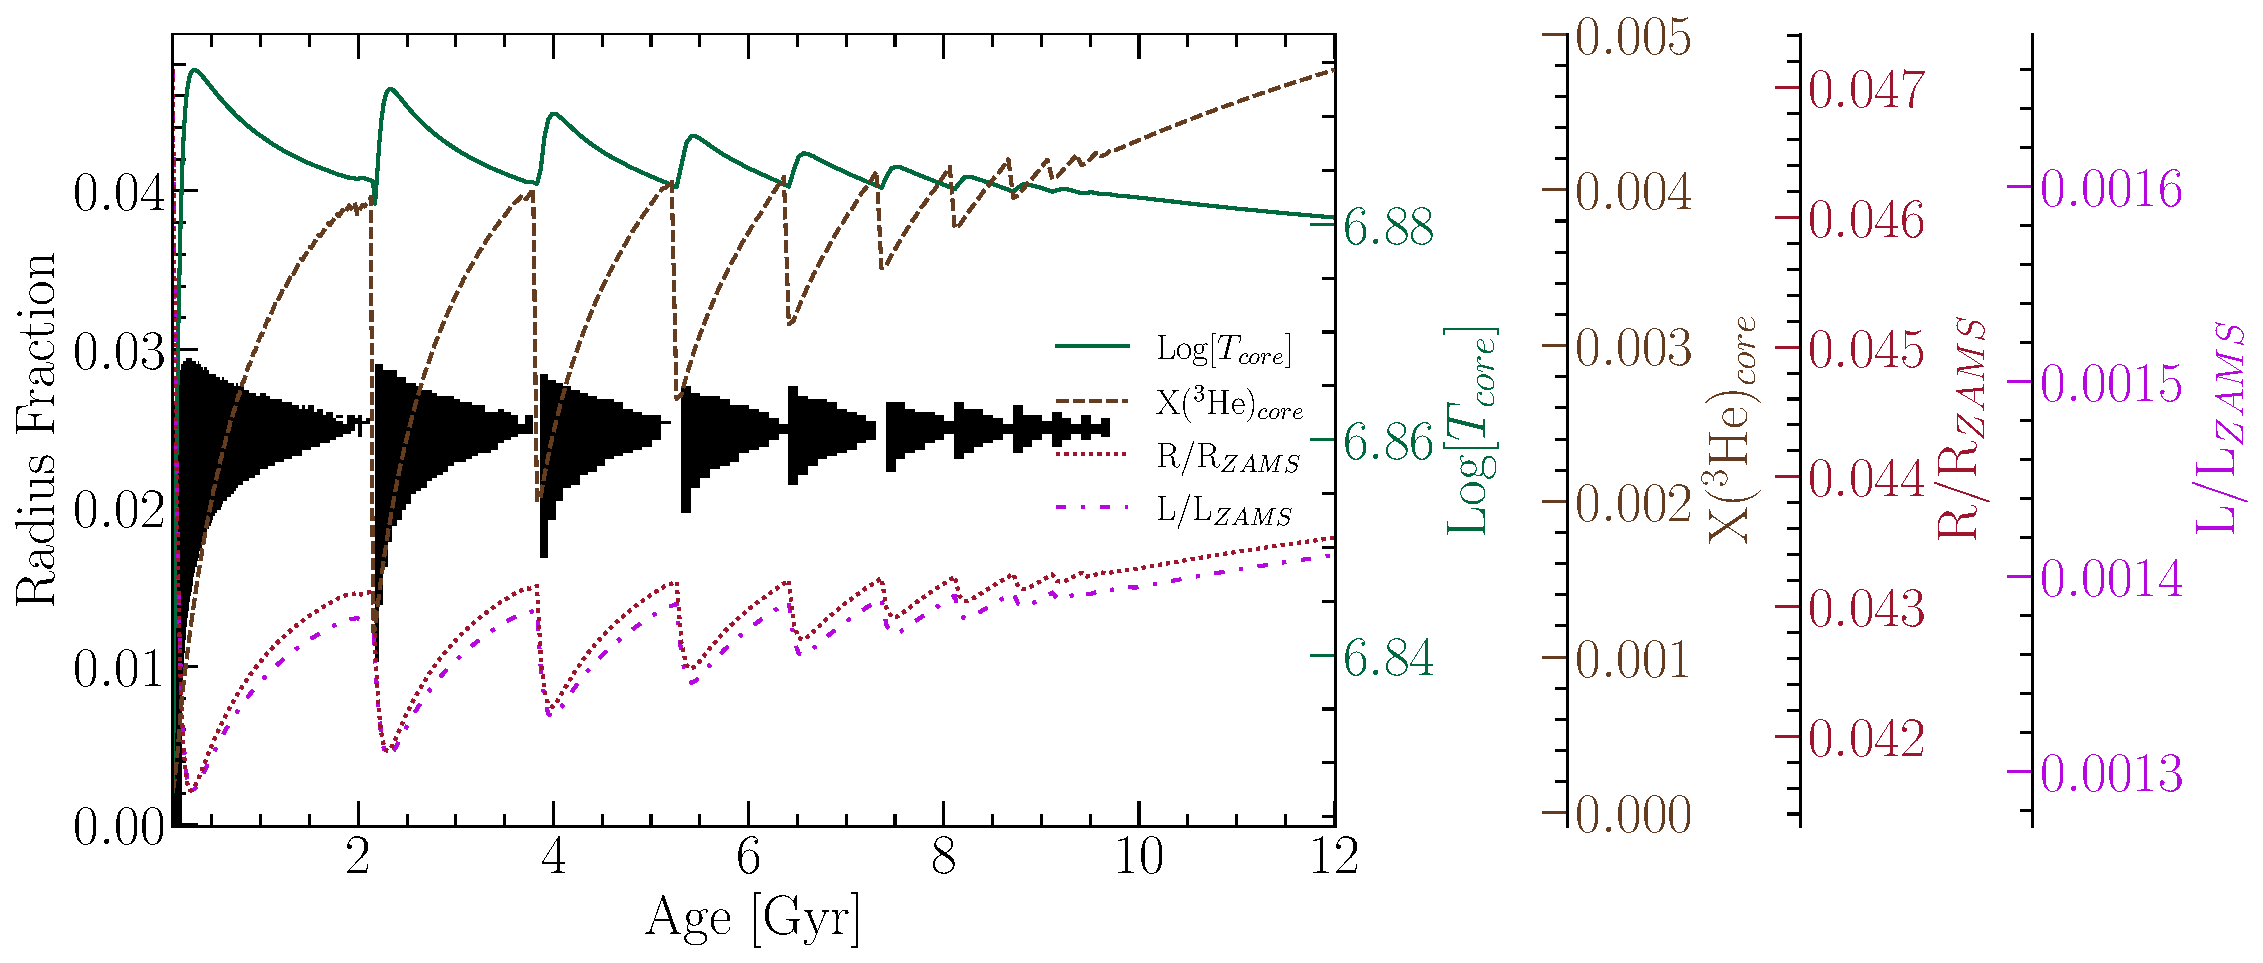
\includegraphics[width=0.95\textwidth]{figures/jaoOpacity/Kippenhan.pdf}
	\caption{Diagram for a characteristic stellar model of 0.35625 $M_{\odot}$
	which is within the Jao Gap's mass range. The black shaded regions denote
	whether, at a particular model age, a radial shell within the model is
	radiative (with white meaning convective). The lines trace the models core
	temperature, core $^{3}$He mass fraction, fractional luminosity wrt. the
	zero age main sequence and fractional radius wrt. the zero age main
	sequence.}
	\label{fig:Kippenhan1}
\end{figure*}


\subsection{Efforts to Model the Gap}
Since the identification of the Gap, stellar modeling has been
conducted to better constrain its location, effects, and exact cause.
Both \citet{Mansfield2021} and \citet{Feiden2021} identify that the Gap's mass
location is correlated with model metallicity --- the mass-luminosity
discontinuity in lower metallicity models being at a commensurately lower mass.
\citet{Feiden2021} suggests this dependence is due to the steep relation of
the radiative temperature gradient, $\nabla_{rad}$, on temperature and, in turn,
on stellar mass.

\begin{align}\label{eqn:radGrad}
	\nabla_{rad} \propto \frac{L\kappa}{T^{4}}
\end{align}

As metallicity decreases so does opacity, which, by Equation \ref{eqn:radGrad},
dramatically lowers the temperature at which radiation will dominate energy
transport \citep{Chabrier1997}. Since main sequence stars are virialized the
core temperature is proportional to the core density and total mass. Therefore,
if the core temperature where convective-kissing instability is expected
decreases with metallicity, so too will the mass of stars which experience such
instabilities.

% \begin{align}\label{eqn:TMRelation}
% 	T_{c} \propto \rho_{c}M^{2}
% \end{align}

The strong opacity dependence of the Jao Gap begs the question: what is
the effect of different opacity calculations on Gap properties.
As we can see above, changing opacity should affect the Gap's location in the
mass-luminosity relation and therefore in a color-magnitude diagram. Moreover,
current models of the Gap have yet to locate it precisely in the CMD
\citep{Feiden2021} with an approximate 0.16 G-magnitude difference between the
observed and modeled Gaps. Opacity provides one, as yet unexplored, parameter
which has the potential to resolve these discrepancies.

\section{Updated Opacities}\label{sec:opac}
% Radiative opacity is fundamental to stellar structure, it determines how much
% incident radiation is absorbed or scattered. Moreover, when a media is in
% thermodynamic equilibrium with the radiation field, that is when the temperature
% of the media and that of the radiation field is the same, the opacity may be
% used via Kirchhoff's law to find the emissivity of a material
% \citep{Huebner2014}. Local Thermodynamic Equilibrium (LTE) is a common state to
% find within a star and therefore stellar models have long relied on opacities
% calculated in LTE.
Multiple groups have released high-temperature opacities including, the Opacity
Project \citep[OP][]{Seaton1994}, Laurence Livermore National Labs OPAL opacity
tables \citep{Iglesias1996}, and Los Alamos National Labs OPLIB opacity tables
\citep{Colgan2016}. OPAL high-temperature radiative opacity tables in
particular are very widely used by current generation isochrone grids
\citep[e.g. Dartmouth, MIST, \& StarEvol, ][]{Dotter2008,Choi2016,Amard2019}.
OPLIB opacity tables \citep{Colgan2016} are not widely used but include the
most up-to-date plasma modeling.

While the overall effect on the CMD of using OPLIB compared to OPAL tables is
small, the strong theoretical opacity dependence of the Jao Gap raises the
potential for these small effects to measurably shift the Gap's location. We
update DSEP to use high temperature opacity tables based on measurements from
Los Alamos national Labs T-1 group \citep[OPLIB,][]{Colgan2016}. The OPLIB
tables are created with ATOMIC \citep{Magee2004,Hakel2006,Fontes2016}, a modern
LTE and non-LTE opacity and plasma modeling code. These updated tables were
initially created in order to incorporate the most up to date plasma
physics at the time \citep{Bahcall2005}. 

OPLIB tables include monochromatic Rosseland mean opacities --- composed from
bound-bound, bound-free, free-free, and scattering opacities --- for elements
hydrogen through zinc over temperatures 0.5eV to 100 keV (5802 K -- 1.16$\times
10 ^{9}$ K) and for mass densities from approximately $10^{-8}$ g cm$^{-3}$ up
to approximately $10^{4}$ g cm$^{-3}$ (though the exact mass density range
varies as a function of temperature). 

DSEP ramps the \citet{Ferguson2005} low temperature opacities to high
temperature opacities tables between $10^{4.3}$ K and $10^{4.5}$ K; therefore,
only differences between high-temperature opacity sources above $10^{4.3}$ K
can effect model evolution. When comparing OPAL and OPLIB opacity tables
(Figure \ref{fig:opacComp}) we find OPLIB opacities are systematically lower
than OPAL opacities for temperatures above $10^{5}$ K. Between $10^{4.3}$ and
$10^{5} K$ OPLIB opacities are larger than OPAL opacities. These generally
lower opacities will decrease the radiative temperature gradient throughout
much of the radius of a model.

\begin{figure}
	\centering
	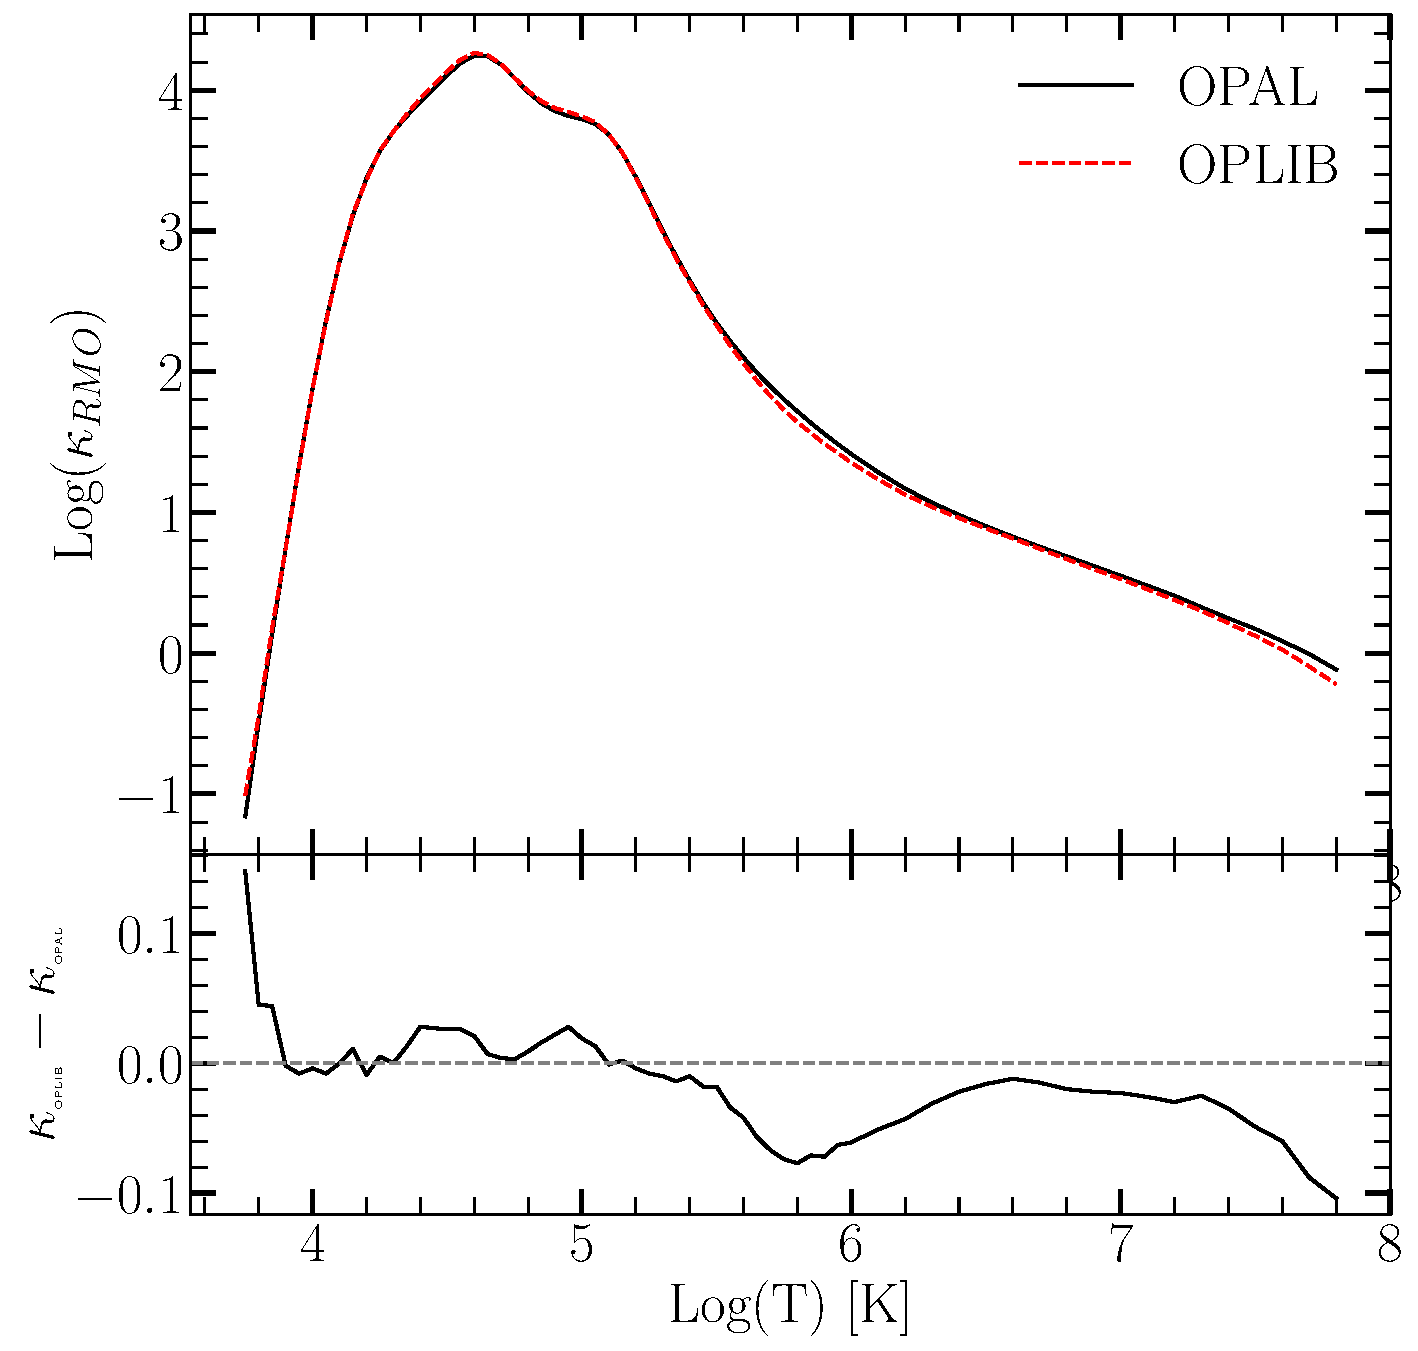
\includegraphics[width=0.45\textwidth]{figures/jaoOpacity/OpacityComparision.pdf}
	\caption{Rosseland mean opacity with the GS98 solar composition for both
	OPAL opacities and OPLIB opacities (top). Residuals between OPLIB opacities
	and OPAL opacities (bottom). These opacities are plotted at $\log _{10}(R)
	= -0.5$, $X=0.7$, and $Z=0.02$. $\log _{10}(R)=-0.5$ approximates
	much of the interior a 0.35 M$_{\odot}$ model. Note how the OPLIB
	opacities are systematically lower than the OPAL opacities for temperatures
	above $10^{5.2}$ K.}
	\label{fig:opacComp}
\end{figure}

\subsection{Table Querying and Conversion}
The high-temperature opacity tables used by DSEP and most other stellar
evolution programs give Rosseland-mean opacity, $\kappa_{R}$, along three
dimensions: temperature, a density proxy $R$ (Equation \ref{eqn:R}; $T_{6} =
T\times10^{-6}$, $\rho$ is the mass density), and composition. 

\begin{align} \label{eqn:R}
	R = \frac{\rho}{T_{6}^{3}}
\end{align}

OPLIB tables may be queried from a web
interface\footnote{https://aphysics2.lanl.gov/apps/}; however, OPLIB opacities
are parametrized using mass-density and temperature instead of $R$ and
temperature. It is most efficient for us to convert these tables to the OPAL
format instead of modifying DSEP to use the OPLIB format directly. In order to
generate many tables easily and quickly we develop a web scraper
\citep[\texttt{pyTOPSScrape},][]{Boudreaux22} which can automatically retrieve
all the tables needed to build an opacity table in the OPAL format.
\texttt{pyTOPSScrape}\footnote{https://github.com/tboudreaux/pytopsscrape} has
been released under the permissive \texttt{MIT} license with the consent of the
Los Alamos T-1 group. For a detailed discussion of how the web scraper works
and how OPLIB tables are transformed into a format DSEP can use see Appendices
\ref{apx:pytopsscrape} \& \ref{apx:interp}.

\subsection{Solar Calibrated Stellar Models}\label{sec:SCSM}
% In order to further validate the OPLIB high-temperature opacities we first visually
% compare a set of opacity vs. temperature curves from OPLIB at a constant $R$
% and \citet{Grevesse1998} composition (GS98) to the same curve from OPAL. A
% characteristic opacity vs temperature curve is shown in Figure
% \ref{fig:OpacCompare}, $\log _{10}(R) = -1.5$ is chosen as for much of the
% radius of a main sequence star $\log _{10}(R)$ is around that value. The
% largest variation in $\kappa_{R}$ from OPAL to OPLIB at $\log _{10}(R)=-1.5$ is
% on the order of a few percent. This is inline with expectations of OPLIB and OPAL
% being in relatively close agreement \citep{Colgan2016}.


In order to validate the OPLIB opacities, we generate a solar calibrated
stellar model (SCSM) using these new tables. We first manually calibrate the
surface Z/X abundance to within one part in 100 of the solar value \citep[][Z/X=0.23]{Grevesse1998}.
Subsequently, we allow both the convective mixing length parameter,
$\alpha_{ML}$, and the initial Hydrogen mass fraction, $X$, to vary
simultaneously, minimizing the difference, to within one part in $10^{5}$,
between resultant models' final radius and luminosity to those of the sun.
Finally, we confirm that the model's surface Z/X abundance is still within one
part in 100 of the solar value.

\begin{figure}
	\centering
	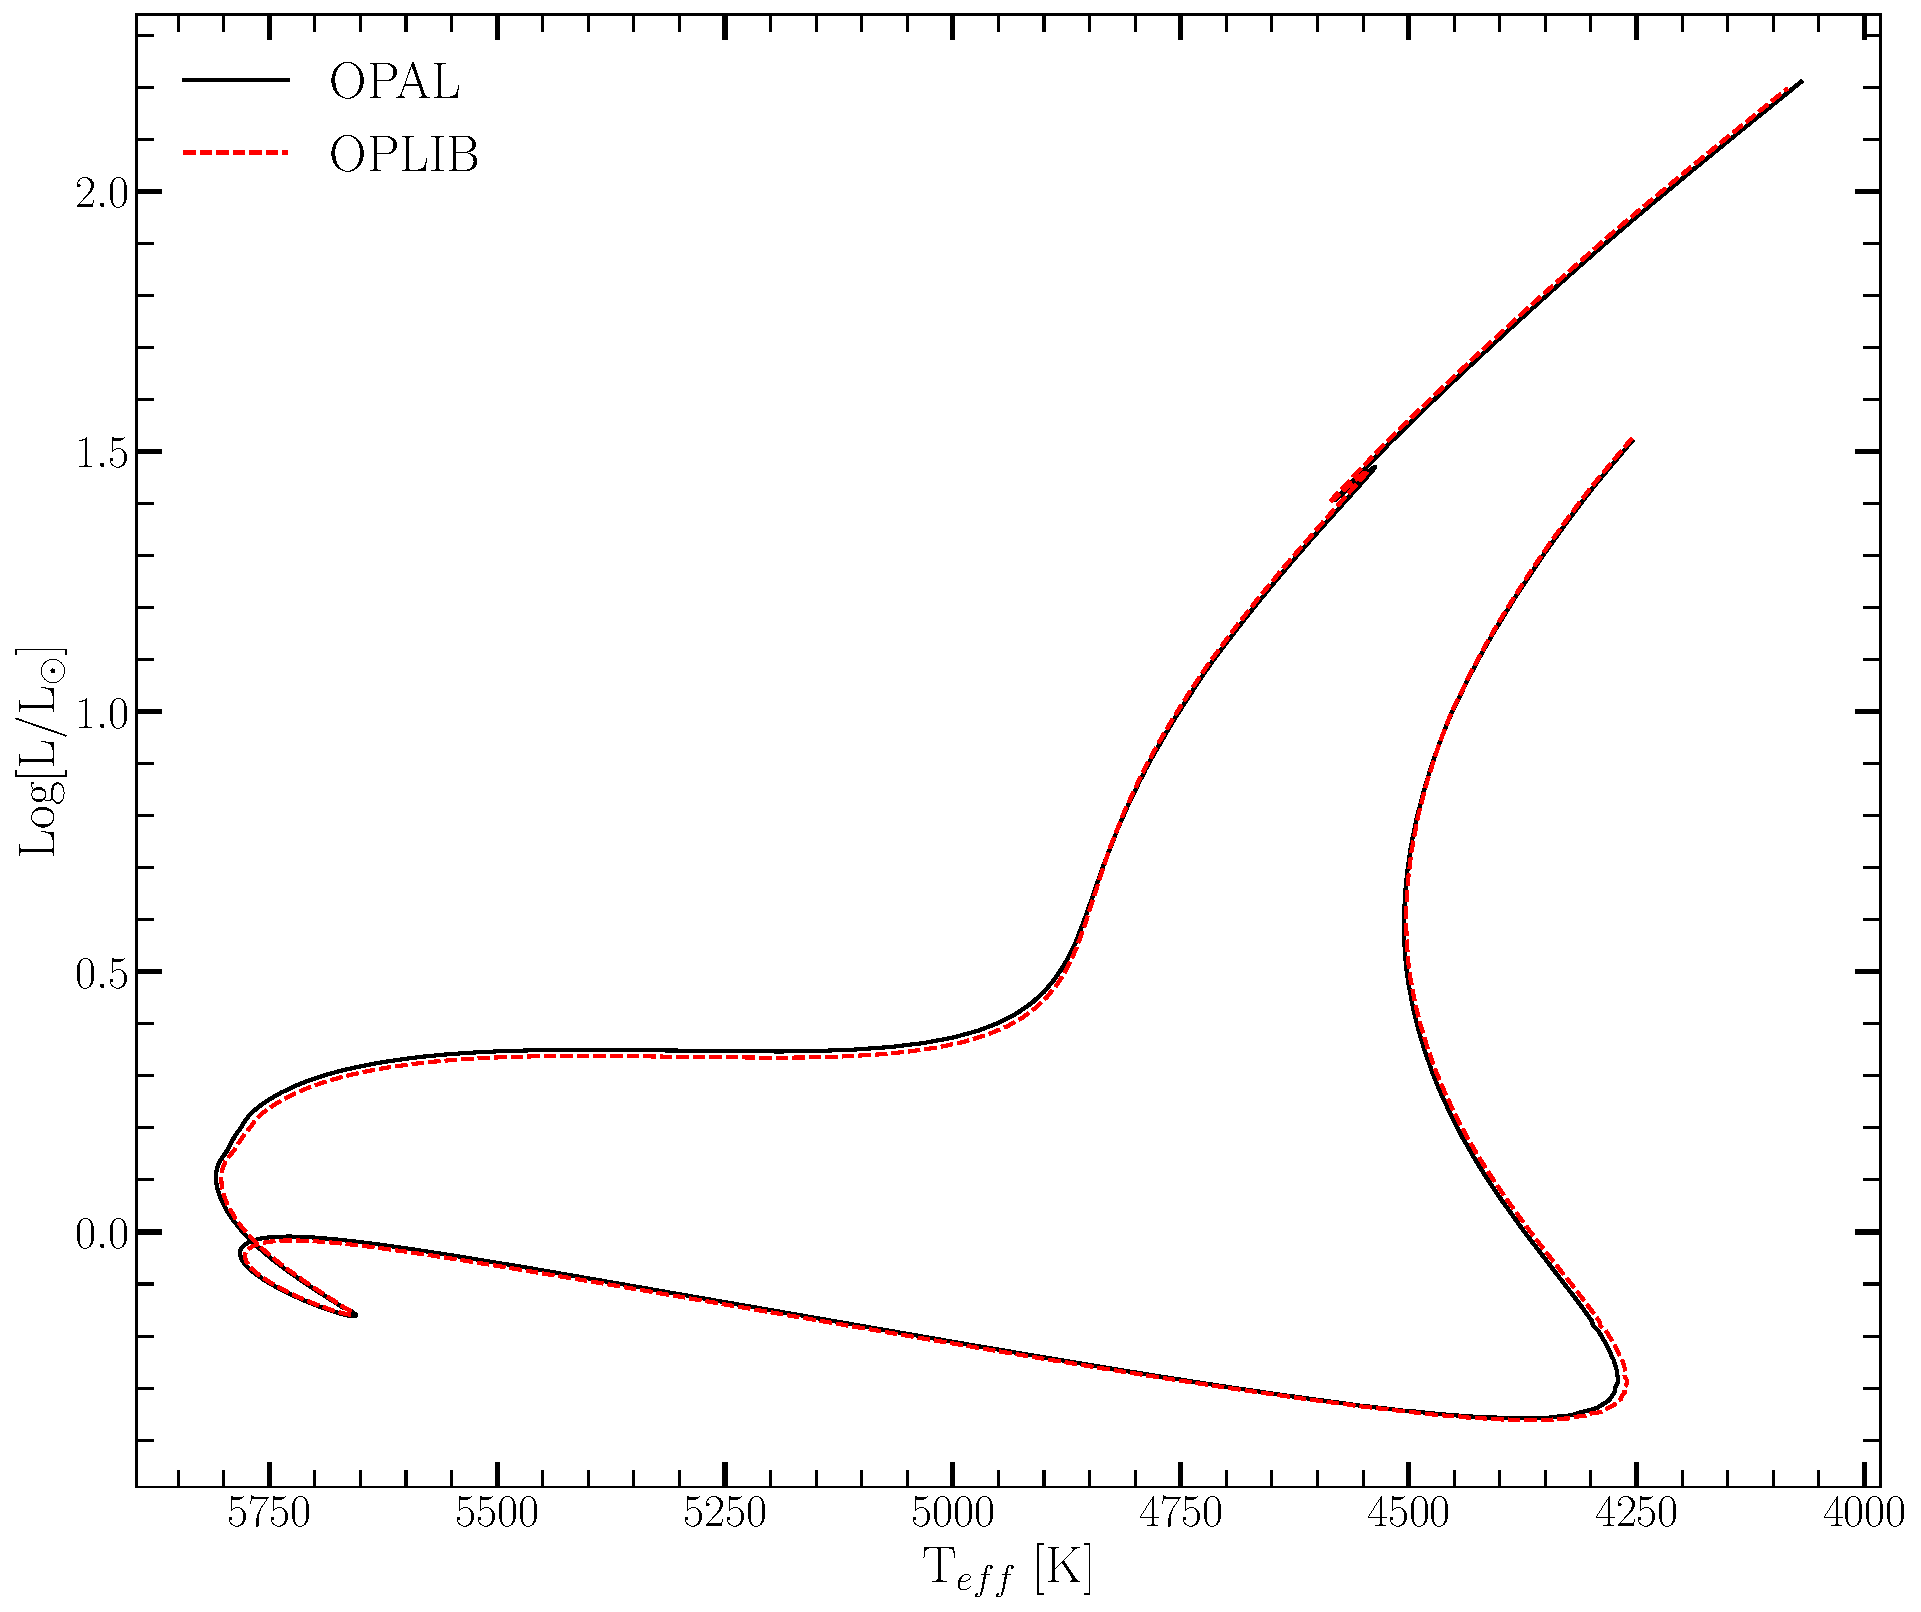
\includegraphics[width=0.45\textwidth]{figures/jaoOpacity/HRDiagramOPALvsOPLIB_SCCM.pdf}
	\caption{HR Diagram for the two SCSMs, OPAL and OPLIB. OPLIB is shown as a red
	dashed line.}
	\label{fig:OPLIBOPALHR}
\end{figure}

Solar calibrated stellar models evolved using GS98 OPAL and OPLIB opacity
tables (Figure \ref{fig:OPLIBOPALHR}) differ $\sim 0.5\%$ in the SCSM hydrogen
mass fractions and $\sim 1.5\%$ in the SCSM convective mixing length parameters
(Table \ref{tab:SCSMResults}). While the two evolutionary tracks are very
similar, note that the OPLIB SCSM's luminosity is systematically lower past the
solar age. While at the solar age the OPLIB SCSM luminosity is effectively the
same as the OPAL SCSM. This luminosity difference between OPAL and OPLIB based
models is not inconsistent with expectations given the more shallow radiative
temperature gradient resulting from the lower OPLIB opacities

\begin{table}
	\centering
	\begin{tabular}{l c c}
		\hline
		Model & $X$ & $\alpha_{ML}$ \\
		\hline
		\hline
		OPAL & 0.7066 & 1.9333 \\
		OPLIB & 0.7107 & 1.9629
	\end{tabular}
	\caption{Optimized parameters for SCSMs evolved using OPAL and OPLIB high
	temperature opacity tables.}
	\label{tab:SCSMResults}
\end{table}


\section{\texttt{pyTOPSScrape}}\label{apx:pytopsscrape}
\texttt{pyTOPSScrape} provides an easy to use command line and python interface
for the OPLIB opacity tables accessed through the TOPS web form. Extensive
documentation of both the command line and programmatic interfaces is linked
in the version controlled repository. However, here we provide a brief,
illustrative, example of potential use.

Assuming \texttt{pyTOPSScrape} has been installed and given some working
directory which contains a file describing a base composition (``comp.dat'')
and another file containing a list of rescalings of that base composition
(``rescalings.dat'') (both of these file formats are described in detail in the
documentation), one can query OPLIB opacity tables and convert them to a form
mimicking that of type 1 OPAL high temperature opacity tables using the
following shell command.

{\small
\begin{verbatim}
	$ generateTOPStables comp.dat rescalings.dat -d ./TOPSCache -o out.opac -j 20
\end{verbatim}
}

\noindent For further examples of pyTOPSScrape please visit the repository.

\section{Interpolating $\rho \rightarrow $ R}\label{apx:interp}
OPLIB parameterizes $\kappa_{R}$ as a function of mass density, temperature in keV,
and composition. Type 1 OPAL high temperature opacity tables, which DSEP and
many other stellar evolution programs use, instead parameterizes opacity as a function
of temperature in Kelvin, $R$ (Equation \ref{eqn:Req}), and composition. The
conversion from temperature in keV to Kelvin is trivial (Equation
\ref{eqn:K2Kev}).
\begin{align}\label{eqn:Req}
	R = \frac{\rho}{T_{6}^{3}}
\end{align}
\begin{align}\label{eqn:K2Kev}
	T_{K} = T_{keV} * 11604525.0061657
\end{align}
However, the conversion from mass density to $R$ is more involved. Because $R$
is coupled with both mass density and temperature there there is no way to
directly convert tabulated values of opacity reported in the OPLIB tables to
their equivalents in $R$ space. The TOPS webform does allow for a
density range to be specified at a specific temperature, which allows for R
values to be directly specified. However, issuing a query to the TOPS webform
for not just every composition in a Type 1 OPAL high temperature opacity table
but also every temperature for every composition will increase the number of
calls to the webform by a factor of 70. Therefore, instead of directly
specifying R through the density range we choose to query tables over a
broad temperature and density range and then rotate these tables,
interpolating $\kappa_{R}(\rho,T_{eff}) \rightarrow \kappa_{R}(R,T_{eff})$. 


To perform this rotation we use the \texttt{interp2d} function within
\texttt{scipy}'s \texttt{interpolate} \citep{2020SciPy-NMeth} module to
construct a cubic bivariate B-spline \citep{Dierckx1981} interpolating function
$s$, with a smoothing factor of 0, representing the surface $\kappa_{R}(\rho,
T_{eff})$. For each $R^{i}$ and $T^{j}_{eff}$ reported in type 1 OPAL tables,
we evaluate Equation \ref{eqn:Req} to find $\rho^{ij} =
\rho(T^{j}_{eff},R^{i})$.  Opacities in $T_{eff}$, $R$ space are then inferred
as $\kappa^{ij}_{R}(R^{i},T^{j}_{eff}) = s(\rho^{ij}, T^{j}_{eff})$. 

As first-order validation of this interpolation scheme we can perform a similar
interpolation in the opposite direction, rotating the tables back to
$\kappa_{R}(\rho, T_{eff})$ and then comparing the initial, ``raw'', opacities
to those which have gone through the interpolations process. Figure
\ref{fig:fracdiff} shows the fractional difference between the raw opacities
and a set which have gone through this double interpolation. The red line
denotes $\log(R)=-0.79$ where models near the Jao Gap mass range will
tend to sit for much of their radius. Along the $\log(R)=-0.79$ line the mean
fractional difference is $\langle \delta \rangle = 0.005$ with an uncertainty of
$\sigma_{\langle\delta\rangle} = 0.013$. One point of note is that, because the
initial rotation into $\log(R)$ space also reduces the domain of the opacity
function, interpolation-edge effects which we avoid initially by extending the
domain past what type 1 OPAL tables include cannot be avoided when
interpolating back into $\rho$ space. 

\begin{figure}
	\centering
	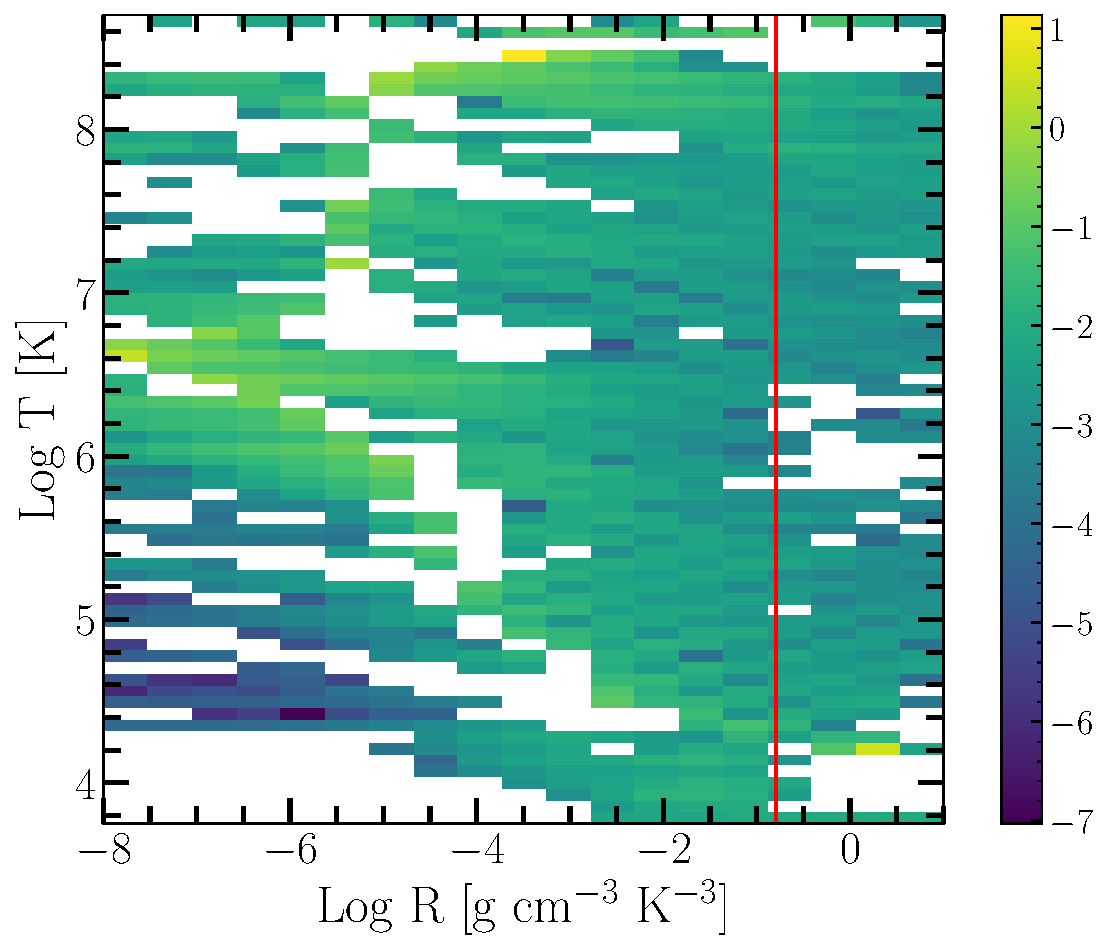
\includegraphics[width=0.85\textwidth]{figures/jaoOpacity/FractionalDifference.pdf}
	\caption{Log Fractional Difference between opacities in $\kappa_{R}(\rho,
	T_{eff})$ space directly queried from the OPLIB web-form and those which
	have been interpolated into $\log(R)$ space and back. Note that, due to the
	temperature grid of type 1 OPAL tables not aligning perfectly which the temperature
	grid OPLIB uses there may be edge effects where the interpolation is poorly
	constrained. The red line corresponds to $\log(R) = -0.79$ where much of a
	stellar model's radius exists.}
	\label{fig:fracdiff}
\end{figure}


\section{Modeling}\label{sec:modeling}
In order to model the Jao Gap we evolve two extremely finely sampled mass grids
of models. One of these grids uses the OPAL high-temperature opacity tables
while the other uses the OPLIB tables (Figure \ref{fig:PunchIn}). Each grid
evolves a model every 0.00025 $M_{\odot}$ from 0.2 to 0.4 $M_{\odot}$ and every
0.005 $M_{\odot}$ from 0.4 to 0.8 $M_{\odot}$. All models in both grids use a
GS98 solar composition, the (1, 101, 0) \texttt{FreeEOS} (version
{\color{red}2.7}) configuration, and 1000 year old pre-main sequence polytropic
models, with polytropic index 1.5, as their initial conditions. We
include gravitational settling in our models where elements are grouped
together. Finally, we set a maximum allowed timestep of 50 million years to
assure that we fully resolve the build of of core $^{3}$He in gap stars.

Despite the alternative view of convection provided by
\citet{MacDonald2018} discussed in Section \ref{sec:JaoGap}, given that the
mixing timescales in these low mass stars are so short \citep[between $10^{7}$s
and $10^{8}$s per][Figure 2 \& Equation 39, which present the
averaged velocity over the convection zone]{Jermyn2022} instantaneous mixing is a valid
approximation. Moreover, one principal motivation for a diffusive model of
convective mixing has been to account for a deuterium concentration gradient
which \citet{Chabrier1997} identify will develop when the deuterium lifetime
against proton capture is significantly shorter than the mixing timescale.
However, the treatment of energy generation used by DSEP \citep{Bahcall2001}
avoides this issue by computing both the equilibrium deuterium abundance and
luminosity of each shell individually, implicitly accounting for the overall
luminosity discrepancy identified by \citeauthor{Chabrier1997}.

Because in this work we are just interested in the location shift of the Gap as
the opacity source varies, we do not model variations in composition.
\citet{Mansfield2021,Jao2020,Feiden2021} all look at the effect composition has
on Jao Gap location. They find that as population metallicity increases so too
does the mass range and consequently the magnitude of the Gap. From an extremely
low metallicity population (Z=0.001) to a population with a more solar like
metallicity this shift in mass range can be up to 0.05 M$_{\odot}$
\citep{Mansfield2021}.

\begin{figure}
	\centering
	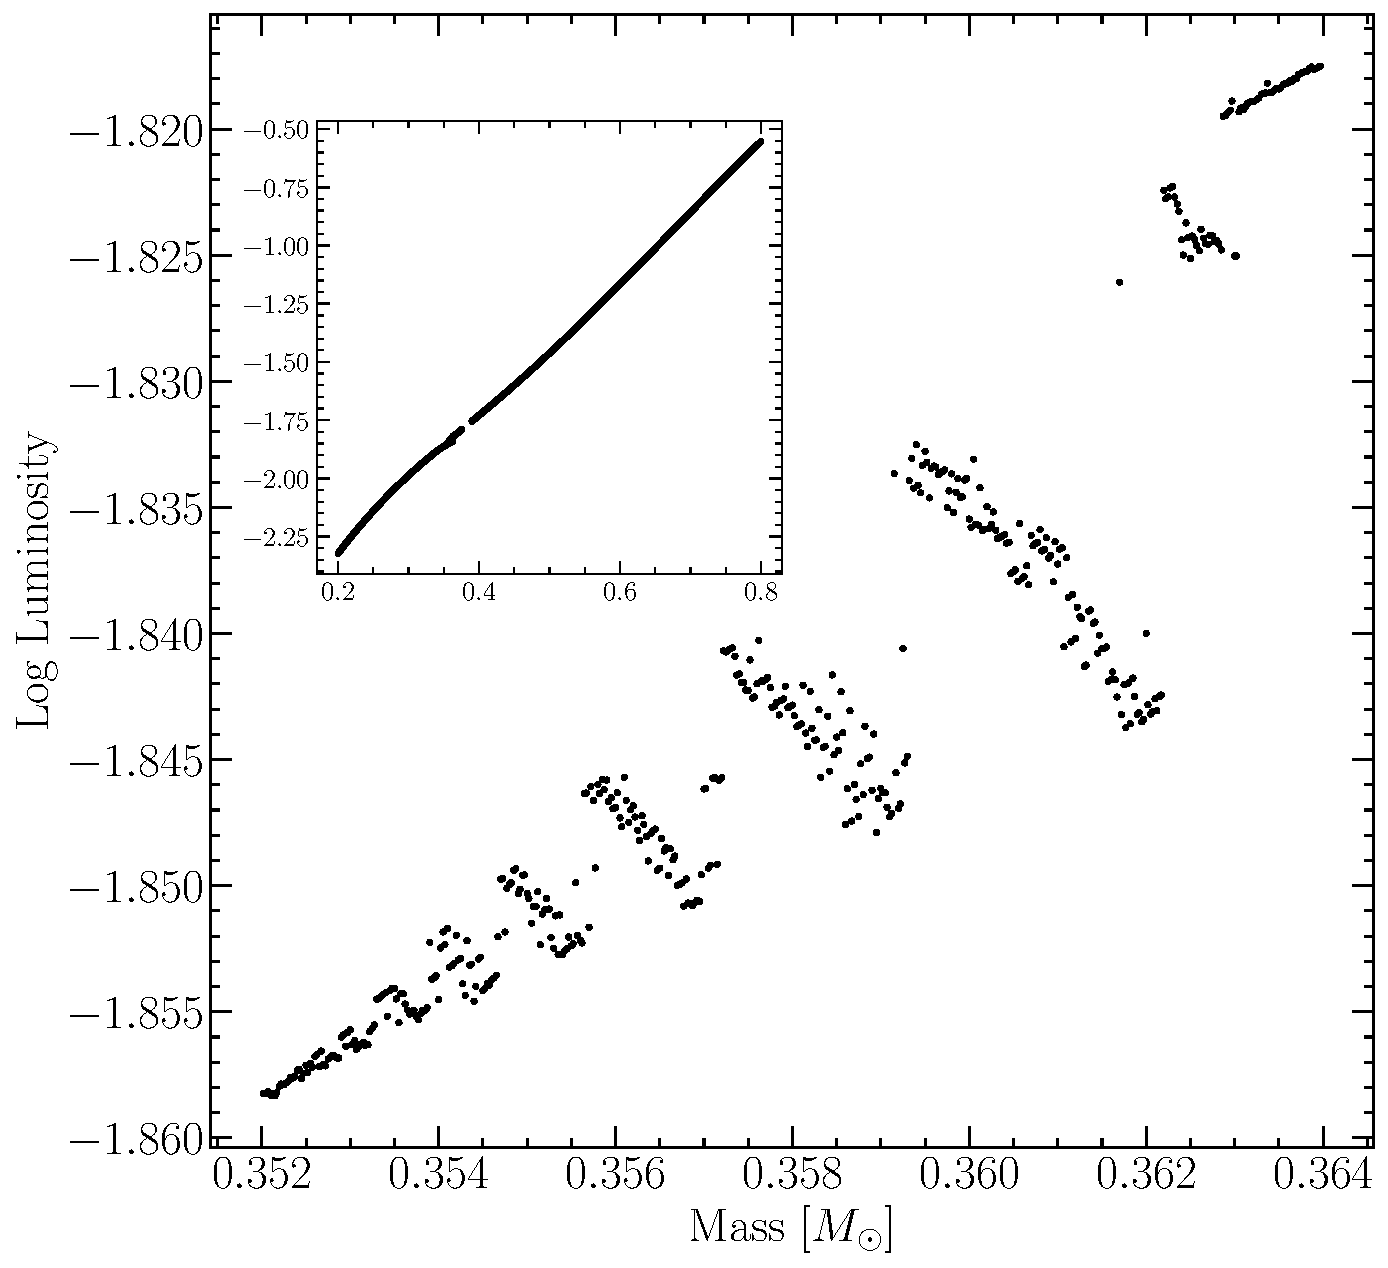
\includegraphics[width=0.85\textwidth]{figures/jaoOpacity/OPALPunchIn.pdf}
	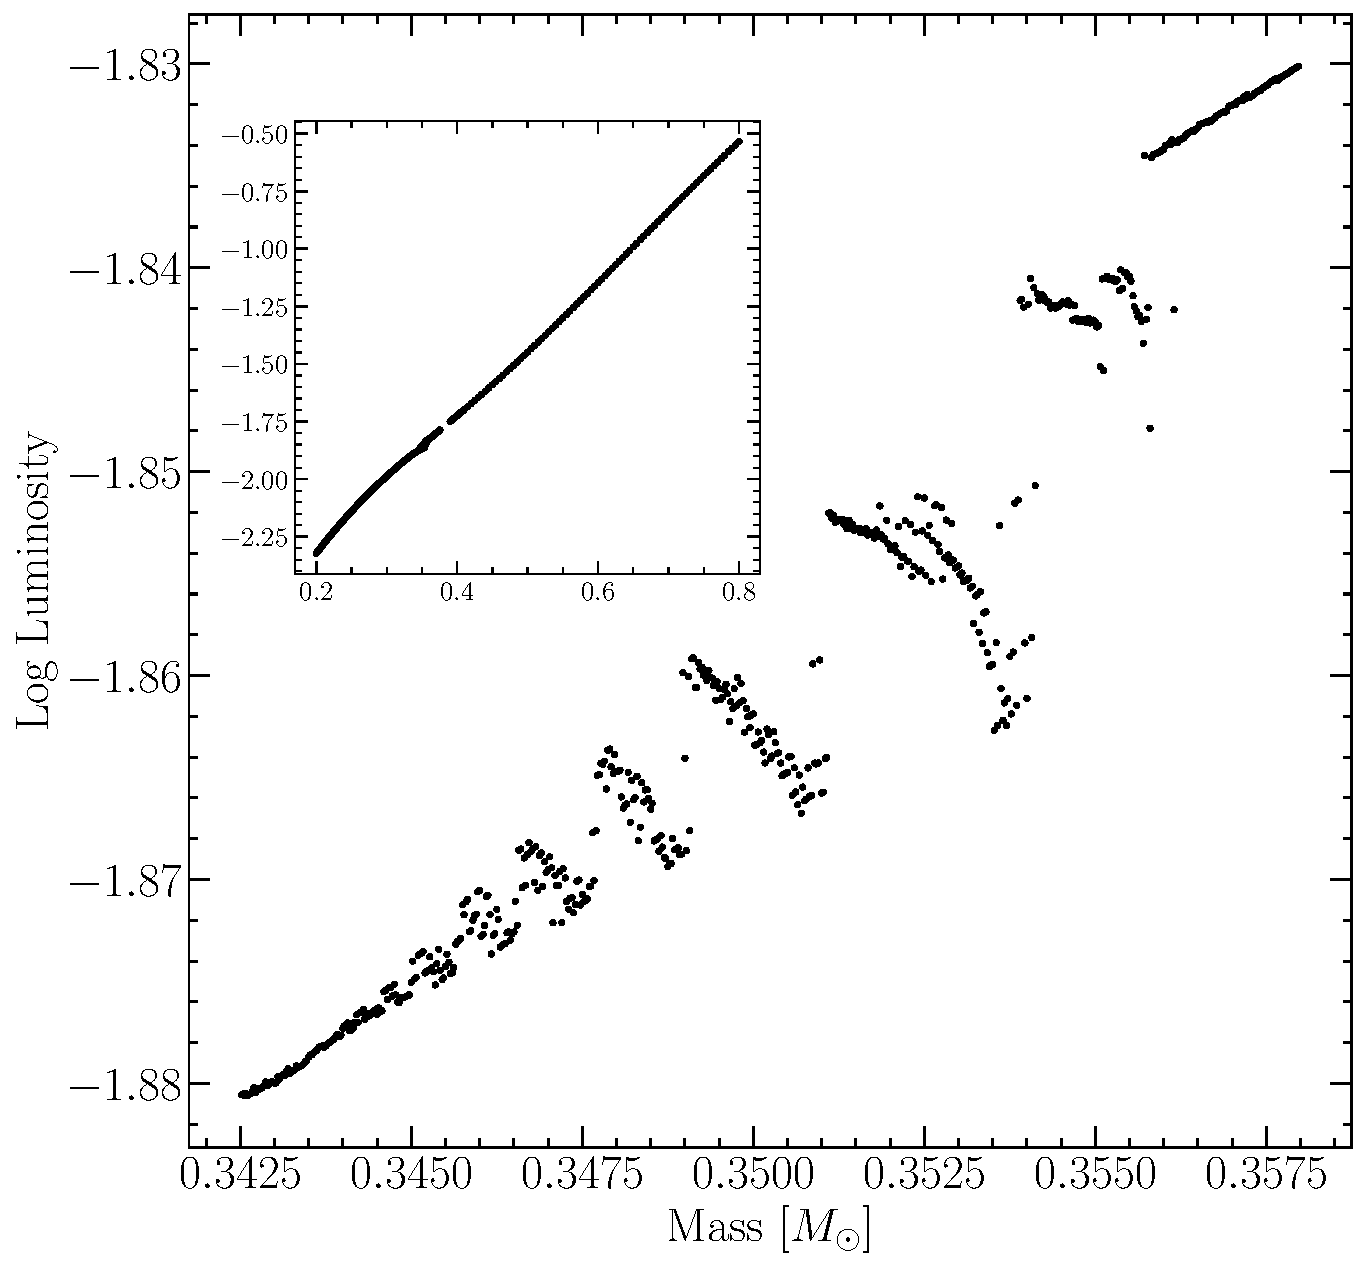
\includegraphics[width=0.85\textwidth]{figures/jaoOpacity/OPLIBPunchIn.pdf}
	\caption{Mass-luminosity relation at 7 Gyrs for models evolved using OPAL opacity
	tables (top) and those evolved using OPLIB opacity tables (bottom). Note
	the lower mass range of the OPLIB Gap.}
	\label{fig:PunchIn}
		
\end{figure}

\subsection{Population Synthesis}
In order to compare the Gap to observations we use in house population
synthesis code. We empirically calibrate the relation between G, BP, and RP
magnitudes and their uncertainties along with the parallax/G magnitude
uncertainty relation using the Gaia Catalouge of Nearby Stas
\citep[GCNS,][]{GaiaCollaboration2021} and Equations \ref{eqn:plxCalib} \&
\ref{eqn:MagCalib}. $M_{g}$ is the Gaia G magnitude while $M_{i}$ is the
magnitude in the i$^\text{th}$ band, G, BP, or RP. The coefficients $a$, $b$,
and $c$ determined using a non-linear least squares fitting routine. Equation
\ref{eqn:plxCalib} then models the relation between G magnitude and parallax
uncertainty while Equation \ref{eqn:MagCalib} models the relation between each
magnitude and its uncertainty.

\begin{align}\label{eqn:plxCalib}
	\sigma_{plx}(M_{g}) = ae^{bM_{g}}+c
\end{align}
\begin{align}\label{eqn:MagCalib}
	\sigma_{i}(M_{i}) = ae^{M_{i}-b}+c
\end{align}

\noindent The full series of steps in our population synthesis code
are:

\begin{figure}
	\centering
	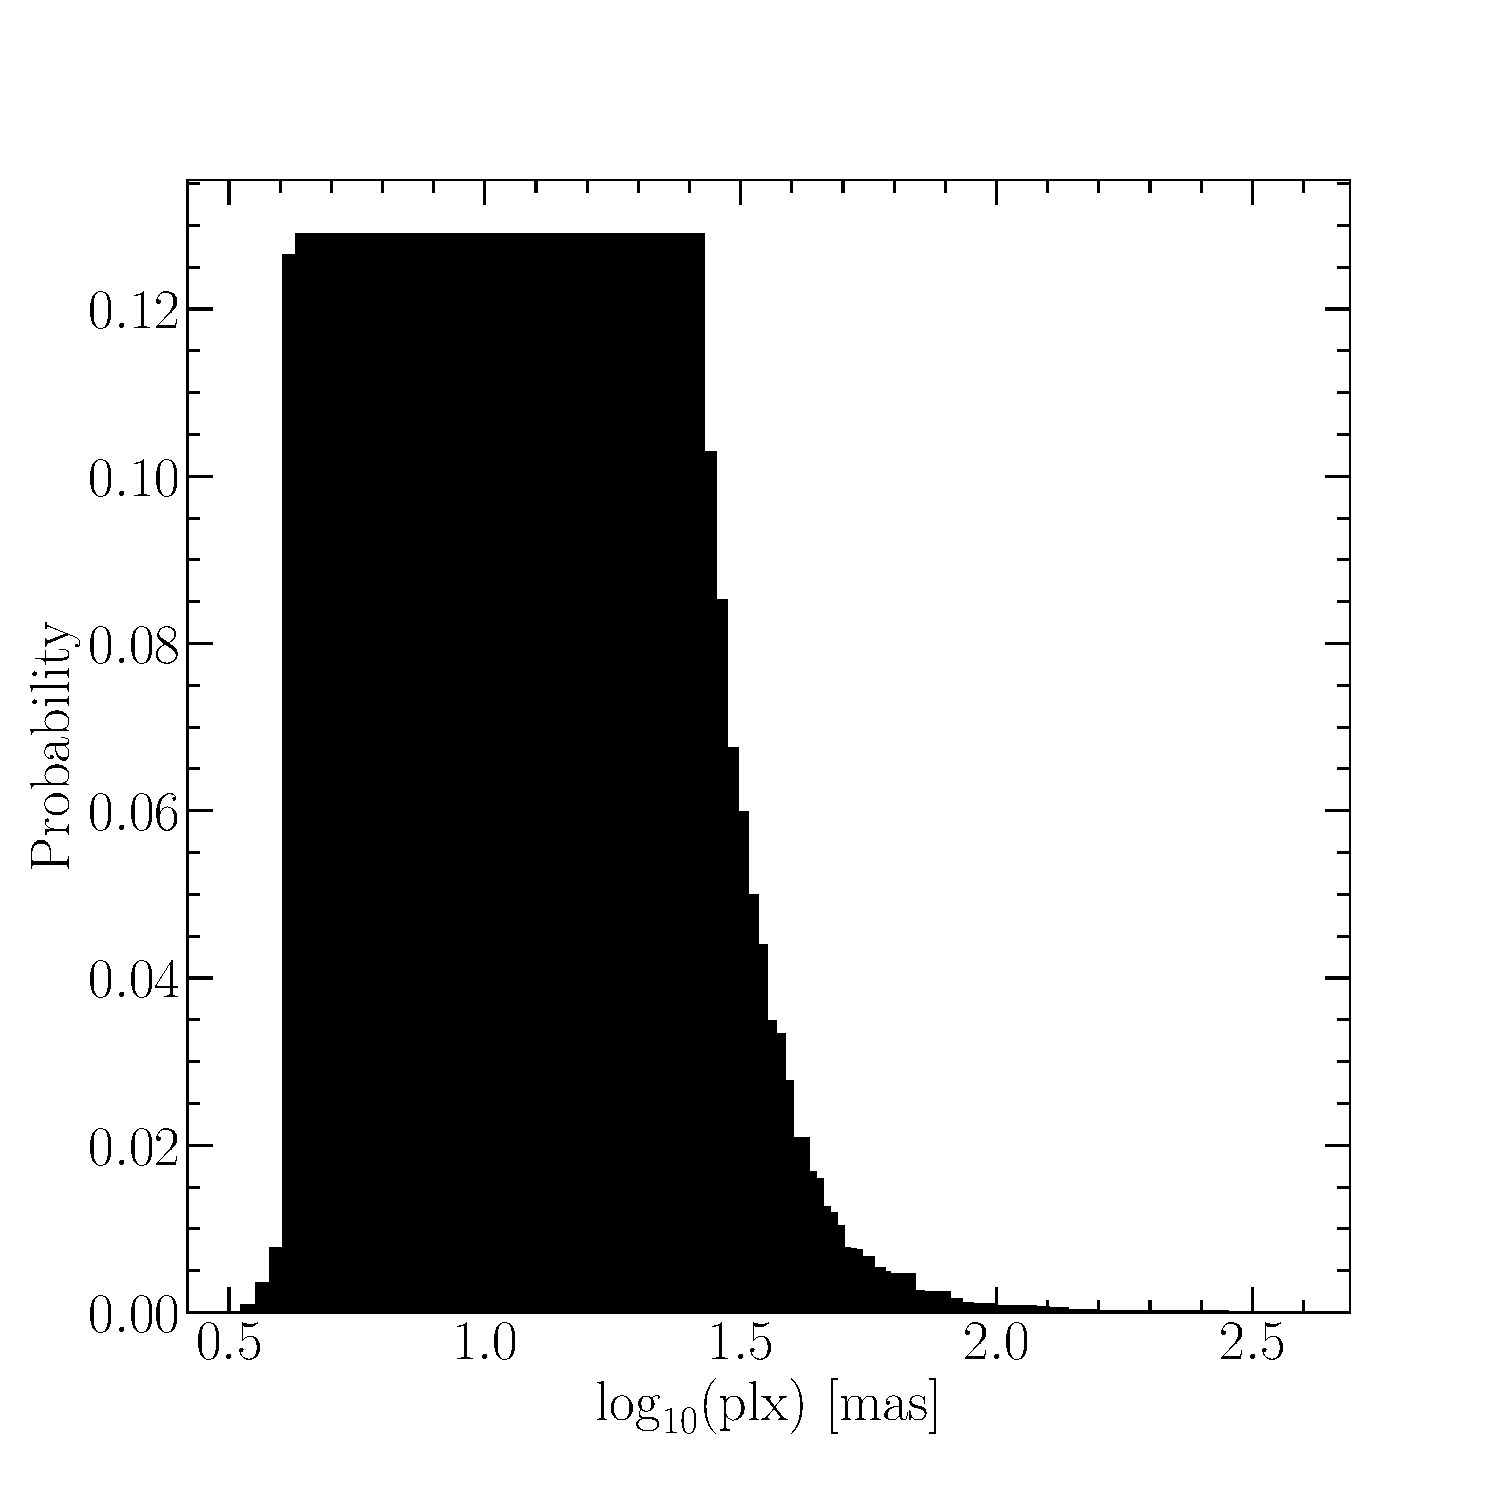
\includegraphics[width=0.85\textwidth]{figures/jaoOpacity/pdist.pdf}
	\caption{Probability distribution sampled when assigning true parallaxes to
	synthetic stars. This distribution is built from the GCNS and includes all
	stars with BP-RP colors between 2.3 and 2.9, the same color range
	of the Jao Gap.}
	\label{fig:pdist}
\end{figure}

\begin{enumerate}
	\item Sample from a \citet{Sollima2019} ($0.25 M_{\odot} < M < 1 M_{\odot}$,
		$\alpha=-1.34\pm0.07$) IMF to determine synthetic star mass.
	\item Find the closest model above and below the synthetic star, lineally
		interpolate these models' $T_{eff}$, $\log(g)$, and $\log(L)$ to those
		at the synthetic star mass.
	\item Convert synthetic star $g$, $T_{eff}$, and $Log(L)$ to Gaia G, BP,
		and RP magnitudes using the Gaia (E)DR3 bolometric corrections
		\citep{Creevey2022} along with code obtained thorough personal
		communication with Aaron Dotter \citep{Choi2016}.
	\item Sample from the GCNS parallax distribution (Figure \ref{fig:pdist}),
		limited to stars within the BP-RP color range of 2.3 -- 2.9, to assign
		synthetic star a ``true'' parallax.
	\item Use the true parallax to find an apparent magnitude for each filter.
	\item Evaluate the empirical calibration given in Equation
		\ref{eqn:plxCalib} to find an associated parallax uncertainty. Then
		sample from a normal distribution with a standard deviation equal to
		that uncertainty to adjust the true parallax resulting in an
		``observed'' parallax.
	\item Use the ``observed'' parallax and the apparent magnitude to find an
		``observed'' magnitude.
	\item Fit the empirical calibration given in Equation \ref{eqn:MagCalib} to
		the GCNS and evaluate it to give a magnitude uncertainty scale in each
		band.
	\item Adjust each magnitude by an amount sampled from a normal
		distribution with a standard deviation of the magnitude uncertainty
		scale found in the previous step.
\end{enumerate}

This method then incorporates both photometric and astrometric uncertainties
into our population synthesis. An example 7 Gyr old synthetic populations
using OPAL and OPLIB opacities are presented in Figure
\ref{fig:PopSynthCompareBasic}.

\begin{figure*}
	\centering
	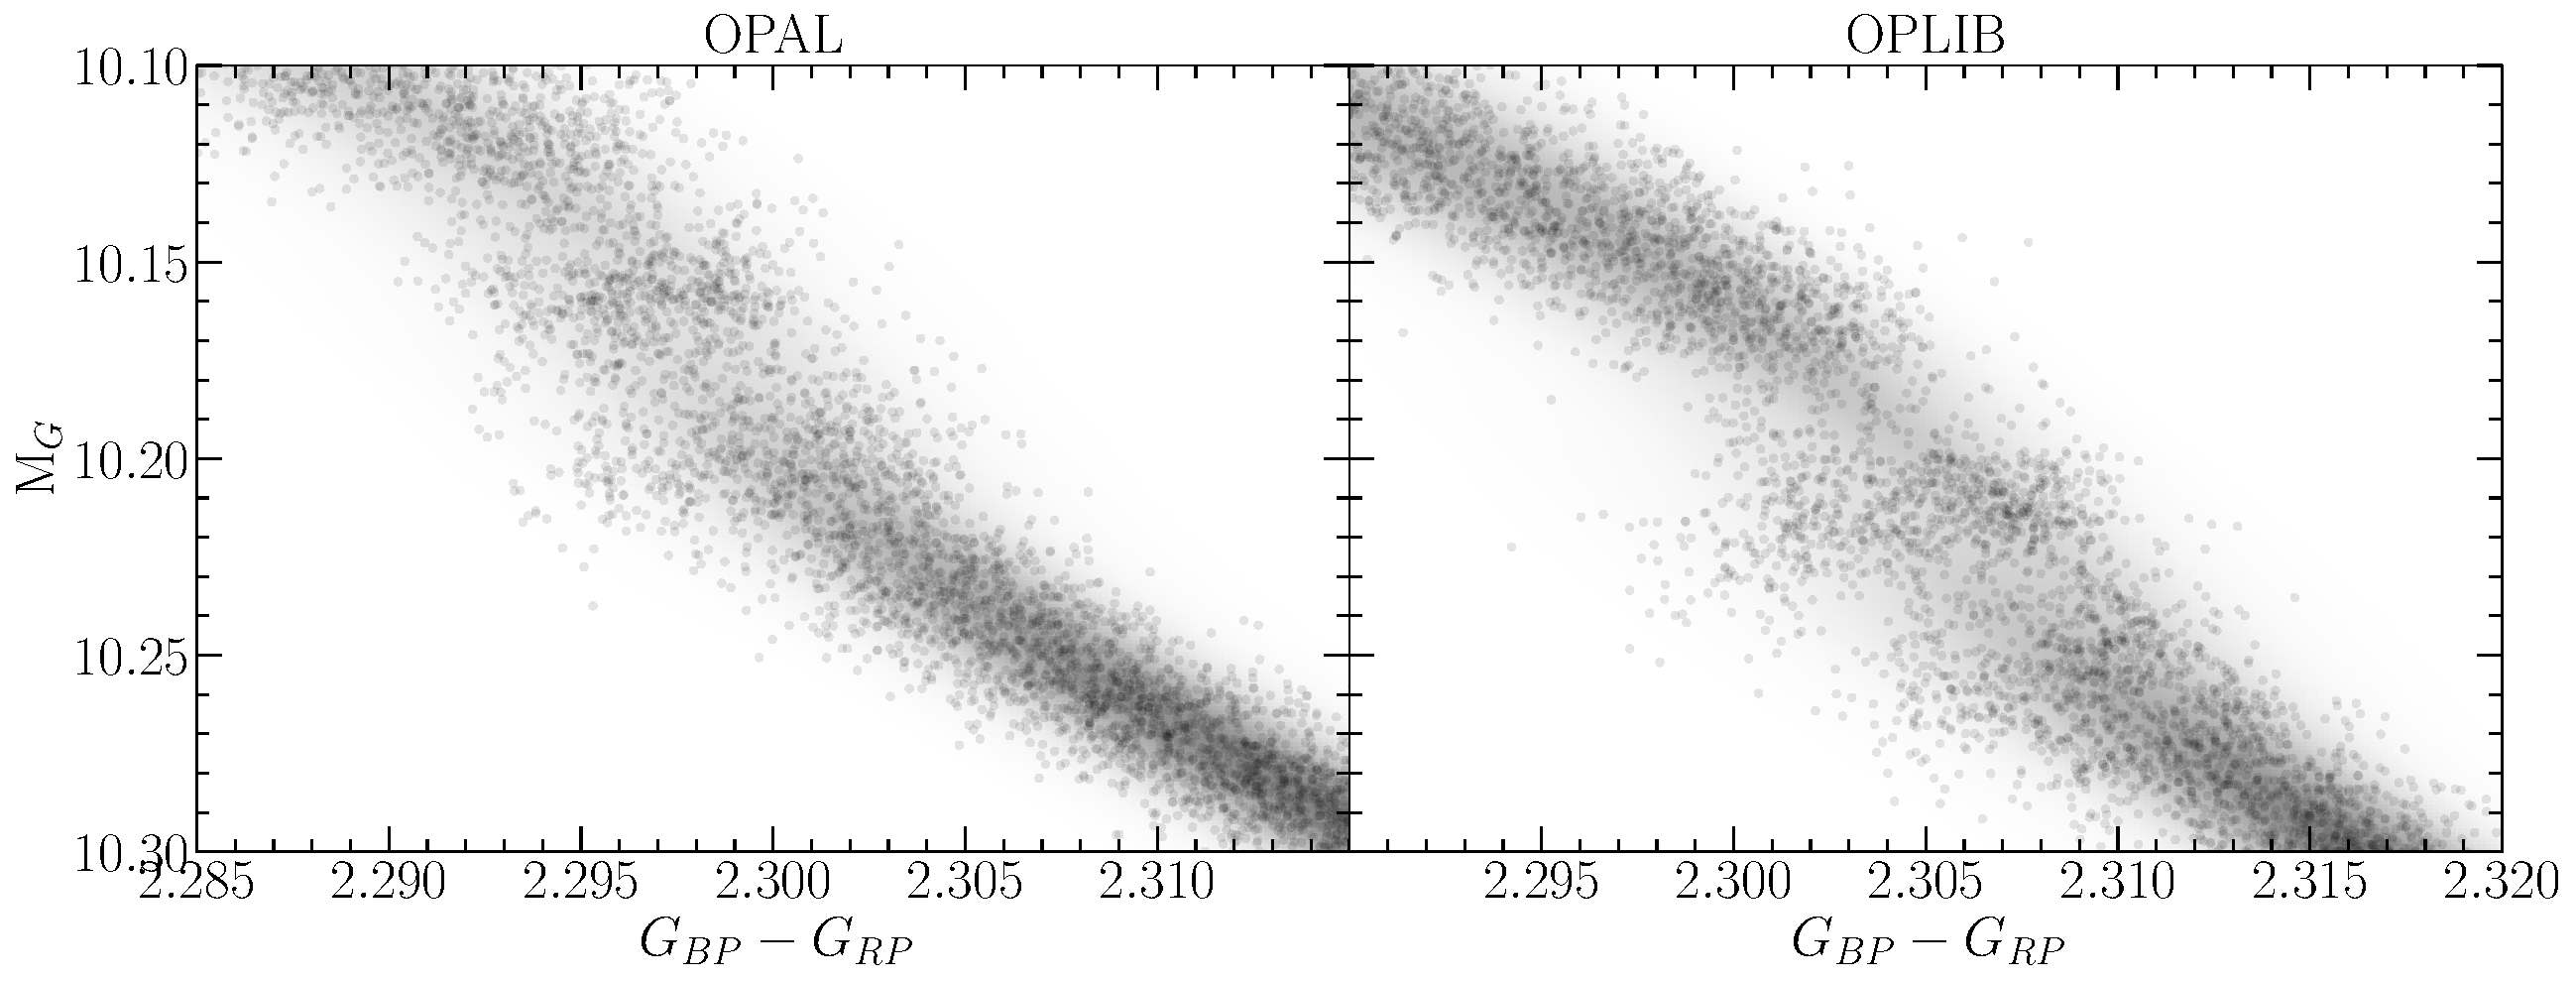
\includegraphics[width=0.85\textwidth]{figures/jaoOpacity/OPALOPLIB_popsynth_compare.pdf}
	\caption{Population synthesis results for models evolved with OPAL (left)
	and models evolved with OPLIB (right). A Gaussian kernel-density estimate
	has been overlaid to better highlight the density variations.}
	\label{fig:PopSynthCompareBasic}
\end{figure*}

\subsection{Mixing Length Dependence}
In order to test the sensitivity of Gap properties to mixing length we
evolve three separate sets OPLIB of models. The first uses a GS98
solar calibrated mixing length, the second uses a mixing length of
1.5, and the third uses a mixing length of 1.0.

We find a clear inverse correlation between mixing length parameter used and
the magnitude of the Jao Gap Figures \ref{fig:MixingLengthCMD} \&
\ref{fig:MixingLengthScaling} ($\mu_{G} \propto -1.5\alpha_{ML}$, where
$\mu_{G}$ is the mean magnitude of the Gap). This is somewhat surprising given
the long established view that the mixing length parameter is of little
relevance in fully convective stars \citep{Baraffe1997}. We find an approximate
0.3 magnitude shift in both the color and magnitude comparing a solar
calibrated mixing length to a mixing length of 1.5, despite only a 16K
difference in effective temperature at 7Gyr between two 0.3 solar mass models.
The slight temperature differences between these models are
attributable to the steeper adiabatic temperature gradients just below the
atmosphere in the solar calibrated mixing length model compared to the
$\alpha_{ML} = 1.5$ model ($\nabla_{ad,solar} - \nabla_{ad,1.5} \approx 0.05$).
Despite this relatively small temperature variance, the large magnitude
difference is expected due to the extreme sensitivity of the bolometric
corrections on effective temperature at these low temperatures. The
mixing length then provides a free parameter which may be used to shift the gap
location in order to better match observations without having a major impact on
the effective temperature of models. Moreover, recent work indicates that using
a solar calibrated mixing length is not appropriate for all stars
\citep[e.g.][]{Trampedach2014, Joyce2018}.

\begin{figure}
	\centering
	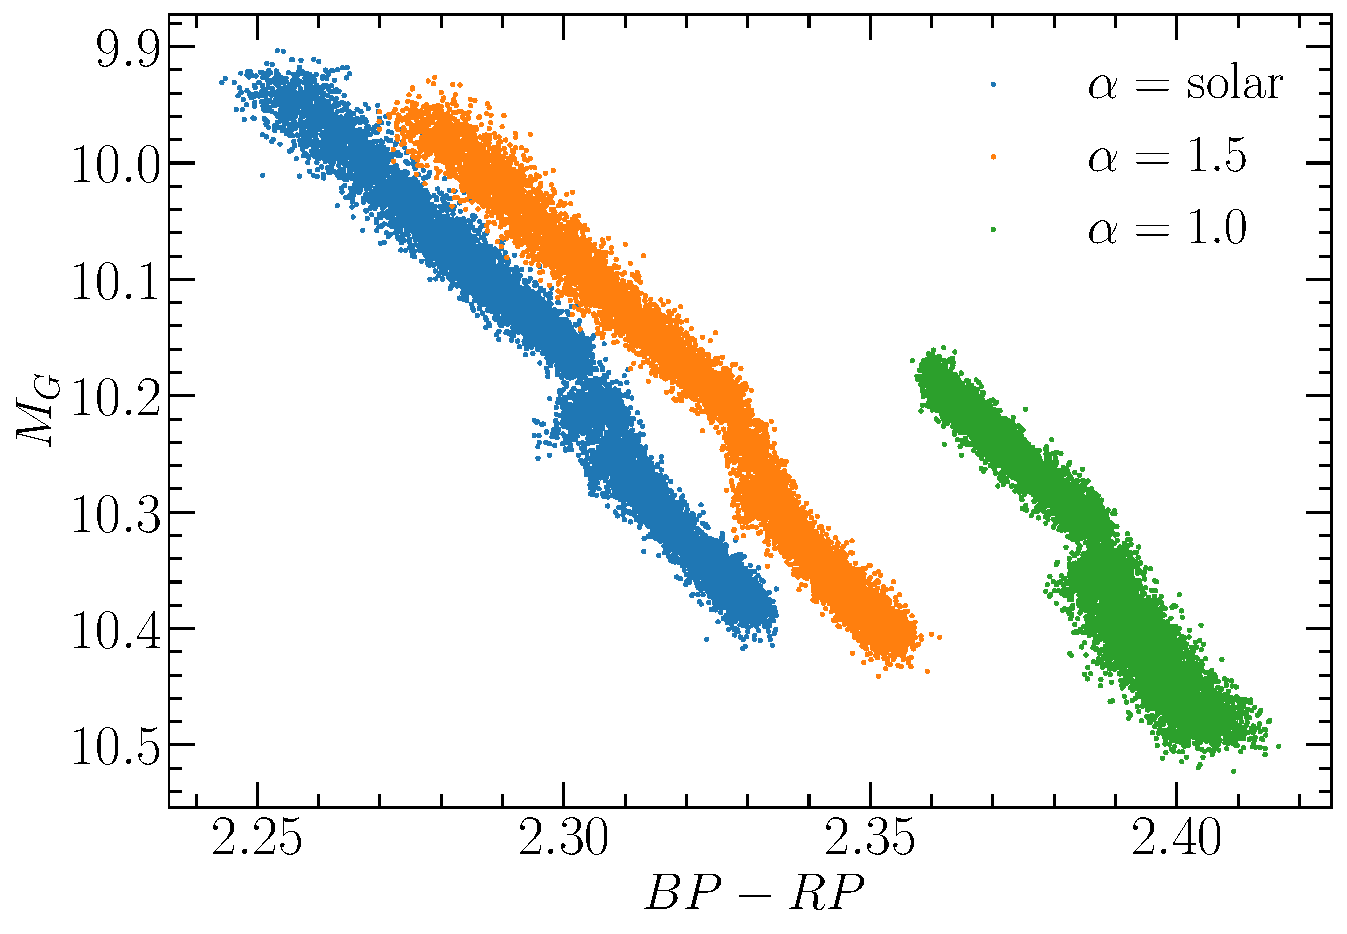
\includegraphics[width=0.85\textwidth]{figures/jaoOpacity/./alphaMLComparisionCMD.pdf}
	\caption{CMD showing OPLIB populations (from left to right) A, B, and C.}
	\label{fig:MixingLengthCMD}
\end{figure}

\begin{figure}
	\centering
	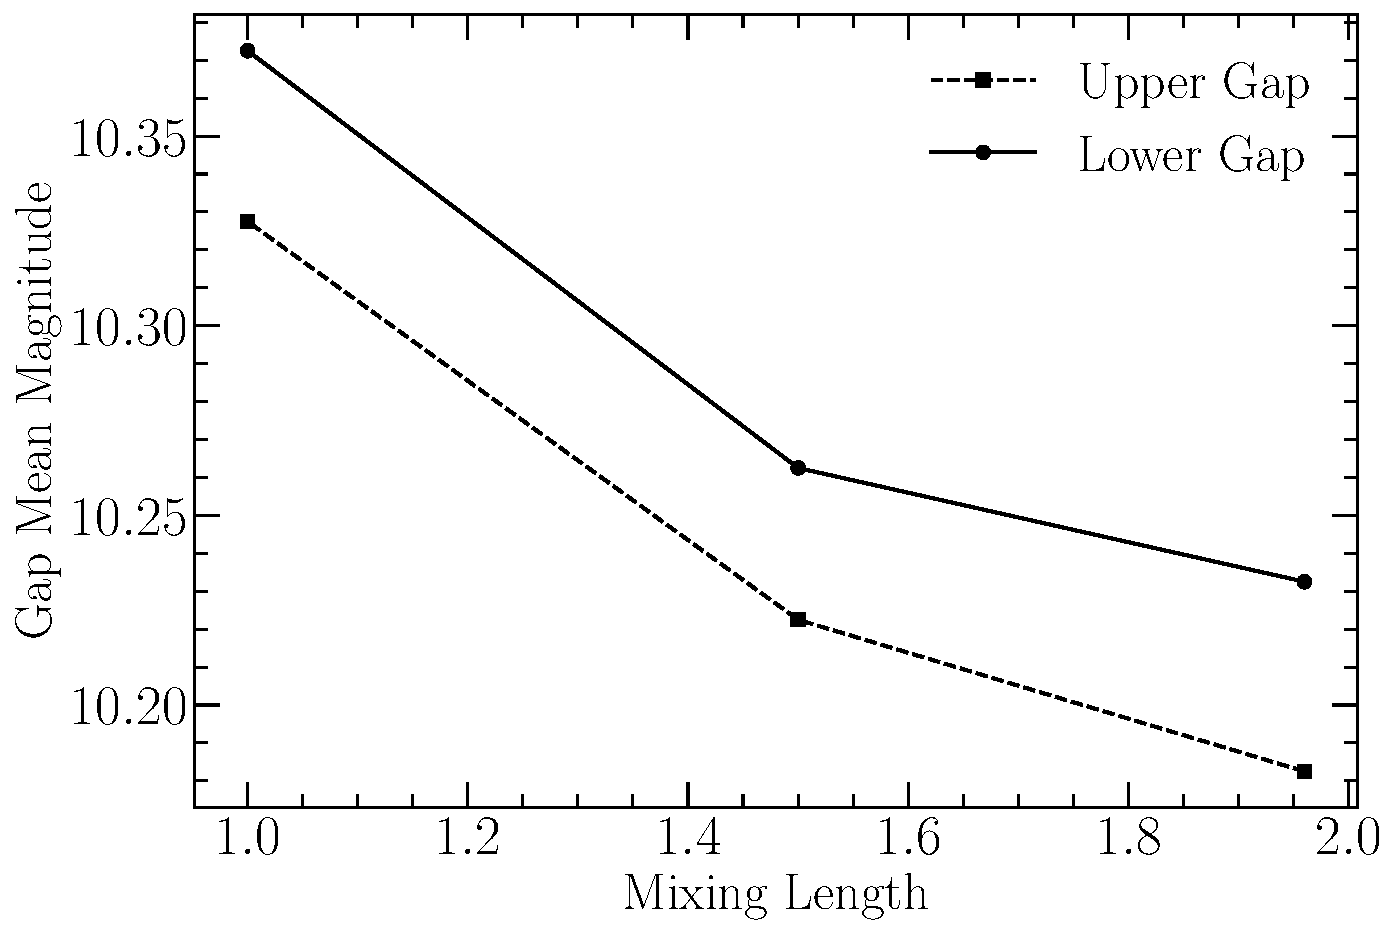
\includegraphics[width=0.85\textwidth]{figures/jaoOpacity/./MixingLengthScaling.pdf}
	\caption{Location of the two identified paucities of stars in OPLIB synthetic
	populations as a function of the mixing length used.}
	\label{fig:MixingLengthScaling}
\end{figure}

Given the variability of gap location with mixing length, it is possible that a
better fit to the gap location may be achieved through adjustment of the
convective mixing length parameter. However, calibrations of the mixing length
for stars other than the sun have focused on stars with effective temperature
at or above that of the sun and there are no current calibrations of the mixing
length parameter for M dwarfs. Moreover, there are additional uncertainties
when comparing the predicted gap location to the measured gap location, such as
those in the conversion from effective temperature, surface gravity, and
luminosity to color, which must be considered if the mixing length is to be
used as a gap location free parameter. Given the dangers of freely adjustable
parameters and the lack of an a priori expectation for what the convective
mixing parameter should be for the population of M Dwarfs in the Gaia DR2 and
EDR3 CMD any attempt to use the Jao Gap magnitude to calibrate a mixing length
value must be done with caution, and take into account the other uncertainties
in the stellar models which could affect the Jao Gap magnitude.


\section{Rotation--Activity Relation}\label{sec:results}
We show our rotation-activity relation in Figures
\ref{fig:RpHKvsRossbySelf} \& \ref{fig:RpHKvsRossbyDef}. Note that
errors are shown in both figures; however, they render smaller than the data
point size. Ca II H\&K is also known to be time variable
\citep[e.g.][]{Baroch2020,Perdelwitz2021}, which is not captured in our
single-epoch data. There is one target cut off by the domain of this graph,
2MASS J10252645+0512391. This target has a measured vsini of $59.5\pm2.1$ km
s$^{-1}$ \citep{Kesseli2018} and is therefore quite rotationally broadened, which
is known to affect $R'_{HK}$ measurements \citep[figure 8]{Schroder2009}. The
data used to generate this figure is given in Table \ref{tab:finalData}. Table
\ref{tab:finalData} includes uncertainties, the R'$_{HK}$ measurements for
stars which did not have photometrically derived rotational periods in MEarth,
and data for 2MASS J10252645+0512391

We find a rotation activity relationship qualitatively similar to that
presented in \citet{Def17}. Our rotation activity relationship exhibits both
the expected saturated and unsaturated regimes --- the flat region at $Ro <
Ro_{s}$ and the sloped region at $Ro \geq Ro_{s}$ respectively. We fit the
rotation activity relation given in Equation \ref{eqn:fitEqn} to our data using
Markov Chain Monte Carlo (MCMC), implemented in \texttt{pymc}
\citep{Salvatier2016}. 

  \begin{equation}\label{eqn:fitEqn}
      \log(R'_{HK}) = \begin{cases}
          \log(R_{s}) & Ro < Ro_{s} \\
          k\log(Ro) + \log(R_{s}) - k\log(Ro_{s}) & Ro \geq Ro_{s}
      \end{cases}
  \end{equation}

\noindent $Ro_{s}$ is the Rossby number cutoff between the saturated and
unsaturated regime. $R_{s}$ is the maximum, saturated, value of $R'_{HK}$ and
$k$ is the index of the power law when $Ro \geq Ro_{s}$. Due to the
issues measuring $R'_{HK}$ for high vsini targets discussed above, we exclude
2MASS J10252645+0512391 from this fit. All logarithms are base ten unless
another base is explicitly given.
\begin{table}[ht]
  \small
    \centering
    \setlength{\tabcolsep}{4pt}
    \begin{tabular}{lcccccccc}
\hline
2MASS ID & Mass & $Ro$ & $\log(R'_{HK})$ & $\log(R'_{HK})_{err}$ & $V_{mag}$ & $V-K$ & prot & $r_{prot}$\\
 & $\mathrm{M_{\odot}}$ &  &  &  & $\mathrm{mag}$ & $\mathrm{mag}$ & $\mathrm{d}$ &   \\
\hline
\hline
06000351+0242236 & 0.24 & 0.020 & -4.5475 & 0.0021 & 11.31 & 5.268 & 1.809 & 2016ApJ...821...93N  \\
02125458+0000167 & 0.27 & 0.048 & -4.6345 & 0.0014 & 13.58 & 5.412 & 4.732 & 2016ApJ...821...93N  \\
01124752+0154395 & 0.28 & 0.026 & -4.4729 & 0.0017 & 14.009 & 5.240 & 2.346 & 2016ApJ...821...93N  \\
10252645+0512391 & 0.11 & 0.000 & -4.9707 & 0.0380 & 18.11 & 7.322 & 0.102 & 2016ApJ...821...93N  \\
05015746-0656459 & 0.17 & 0.873 & -5.0049 & 0.0028 & 12.2 & 5.464 & 88.500 & 2012AcA....62...67K  \\
06022261-2019447 & 0.23 & 1.307 & -5.6980 & 0.0192 & 13.26 & 4.886 & 95.000 & This Work  \\
06105288-4324178 & 0.30 & 0.705 & -5.2507 & 0.0139 & 12.28 & 4.968 & 53.736 & 2018AJ....156..217N  \\
09442373-7358382 & 0.24 & 0.542 & -5.6026 & 0.0147 & 15.17 & 5.795 & 66.447 & 2018AJ....156..217N  \\
14211512-0107199 & 0.24 & 1.160 & -5.5846 & 0.0125 & 13.12 & 5.027 & 91.426 & 2018AJ....156..217N  \\
14294291-6240465 & 0.12 & 0.394 & -5.0053 & 0.0014 & 11.13 & 6.746 & 83.500 & 1998AJ....116..429B  \\
16352464-2718533 & 0.23 & 1.423 & -5.5959 & 0.0108 & 14.18 & 5.182 & 122.656 & 2018AJ....156..217N  \\
16570570-0420559 & 0.24 & 0.014 & -4.3071 & 0.0014 & 12.25 & 5.130 & 1.212 & 2012AcA....62...67K  \\
02004725-1021209 & 0.34 & 0.188 & -4.7907 & 0.0026 & 14.118 & 5.026 & 14.793 & 2018AJ....156..217N  \\
18494929-2350101 & 0.18 & 0.034 & -4.5243 & 0.0015 & 10.5 & 5.130 & 2.869 & 2007AcA....57..149K  \\
20035892-0807472 & 0.33 & 0.946 & -5.6530 & 0.0077 & 13.54 & 5.254 & 84.991 & 2018AJ....156..217N  \\
21390081-2409280 & 0.21 & 1.152 & -6.1949 & 0.0190 & 13.45 & 5.091 & 94.254 & 2018AJ....156..217N  \\
23071524-2307533 & 0.30 & 0.720 & -5.2780 & 0.0077 & 13.587 & 4.849 & 51.204 & 2018AJ....156..217N  \\
00094508-4201396 & 0.30 & 0.009 & -4.3392 & 0.0018 & 13.62 & 5.397 & 0.859 & 2018AJ....156..217N  \\
00310412-7201061 & 0.31 & 0.906 & -5.3879 & 0.0074 & 13.69 & 5.245 & 80.969 & 2018AJ....156..217N  \\
01040695-6522272 & 0.17 & 0.006 & -4.4889 & 0.0024 & 13.98 & 5.448 & 0.624 & 2018AJ....156..217N  \\
02014384-1017295 & 0.19 & 0.034 & -4.5400 & 0.0022 & 14.473 & 5.284 & 3.152 & 2018AJ....156..217N  \\
03100305-2341308 & 0.40 & 0.028 & -4.2336 & 0.0017 & 13.502 & 4.935 & 2.083 & 2018AJ....156..217N  \\
03205178-6351524 & 0.33 & 1.029 & -5.6288 & 0.0096 & 13.433 & 5.238 & 91.622 & 2018AJ....156..217N  \\
07401183-4257406 & 0.15 & 0.002 & -4.3365 & 0.0022 & 13.81 & 6.042 & 0.307 & 2018AJ....156..217N  \\
08184619-4806172 & 0.37 & 0.021 & -4.2834 & 0.0025 & 14.37 & 5.019 & 1.653 & 2018AJ....156..217N  \\
08443891-4805218 & 0.20 & 1.348 & -5.6682 & 0.0067 & 13.932 & 5.370 & 129.513 & 2018AJ....156..217N  \\
09342791-2643267 & 0.19 & 0.007 & -4.3415 & 0.0025 & 13.992 & 5.373 & 0.694 & 2018AJ....156..217N  \\
09524176-1536137 & 0.26 & 1.342 & -5.6319 & 0.0110 & 13.43 & 4.923 & 99.662 & 2018AJ....156..217N  \\
11075025-3421003 & 0.25 & 0.068 & -4.2250 & 0.0032 & 15.04 & 5.633 & 7.611 & 2018AJ....156..217N  \\
11575352-2349007 & 0.39 & 0.031 & -4.2952 & 0.0026 & 14.77 & 5.415 & 3.067 & 2018AJ....156..217N  \\
12102834-1310234 & 0.36 & 0.435 & -4.6892 & 0.0029 & 13.83 & 5.418 & 42.985 & 2018AJ....156..217N  \\
12440075-1110302 & 0.18 & 0.020 & -4.4053 & 0.0033 & 14.22 & 5.546 & 2.099 & 2018AJ....156..217N  \\
13442092-2618350 & 0.35 & 2.032 & -5.9634 & 0.0253 & 13.253 & 4.968 & 154.885 & 2018AJ....156..217N  \\
14253413-1148515 & 0.51 & 0.301 & -4.7641 & 0.0030 & 13.512 & 5.121 & 25.012 & 2018AJ....156..217N  \\
14340491-1824106 & 0.38 & 0.271 & -4.6093 & 0.0038 & 14.346 & 5.638 & 30.396 & 2018AJ....156..217N  \\
15154371-0725208 & 0.38 & 0.050 & -4.6214 & 0.0023 & 12.93 & 5.224 & 4.379 & 2018AJ....156..217N  \\
15290145-0612461 & 0.46 & 0.095 & -4.2015 & 0.0017 & 14.011 & 5.230 & 8.434 & 2018AJ....156..217N  \\
16204186-2005139 & 0.45 & 0.031 & -4.3900 & 0.0035 & 13.68 & 5.261 & 2.814 & 2018AJ....156..217N  \\
16475517-6509116 & 0.17 & 0.889 & -4.8744 & 0.0045 & 13.98 & 5.101 & 73.142 & 2018AJ....156..217N  \\
20091824-0113377 & 0.15 & 0.010 & -4.3772 & 0.0023 & 14.47 & 5.958 & 1.374 & 2018AJ....156..217N  \\
20273733-5452592 & 0.35 & 1.520 & -5.9982 & 0.0181 & 13.18 & 5.259 & 136.924 & 2018AJ....156..217N  \\
20444800-1453208 & 0.49 & 0.073 & -4.4912 & 0.0023 & 14.445 & 5.305 & 6.715 & 2018AJ....156..217N  \\
15404341-5101357 & 0.10 & 0.318 & -5.0062 & 0.0081 & 15.26 & 7.317 & 93.702 & 2018AJ....156..217N  \\
22480446-2422075 & 0.20 & 0.005 & -4.4123 & 0.0016 & 12.59 & 5.384 & 0.466 & 2013AJ....146..154M  \\
06393742-2101333 & 0.26 & 0.952 & -5.2524 & 0.0069 & 12.77 & 5.120 & 79.152 & 2018AJ....156..217N  \\
04130560+1514520 & 0.30 & 0.019 & -4.4775 & 0.0088 & 15.881 & 5.437 & 1.881 & 2016ApJ...818..46M  \\
02411510-0432177 & 0.20 & 0.004 & -4.4272 & 0.0016 & 13.79 & 5.544 & 0.400 & 2020ApJ...905..107M  \\
  11381671-7721484 & 0.12 & 0.958 & \textbf{-5.5015} & 0.0369 & 14.78 & 6.259 & 153.506 & This Work  \\
  12384914-3822527 & 0.15 & 2.527 & \textbf{-6.0690} & 0.0156 & 12.75 & 5.364 & 241.913 & This Work  \\
  13464102-5830117 & 0.48 & 1.340 & \textbf{-5.6977} & 0.0146 &  &  & 65.017 & This Work  \\
  15165576-0037116 & 0.31 & 0.157 & \textbf{-4.0704} & 0.0024 & 14.469 & 5.364 & 15.028 & This Work  \\
  19204795-4533283 & 0.18 & 1.706 & \textbf{-5.8392} & 0.0091 & 12.25 & 5.405 & 167.225 & This Work  \\
  21362532-4401005 & 0.20 & 1.886 & \textbf{-5.8978} & 0.0168 & 14.14 & 5.610 & 207.983 & This Work  \\
\hline
\end{tabular}


% \begin{tabular}{lcccccc}
% \hline
% 	2MASS ID &  Mass &    $Ro$ &  $\log(R'_{HK})$ & $\log(R'_{HK})_{err}$ & $V_{mag}$ &   $V-K$ \\
% \hline
% \hline
% 06000351+0242236 &  0.237 &  0.020 &     -4.548 &          0.002 &  11.310 &  5.268 \\
% 02125458+0000167 &  0.268 &  0.048 &     -4.635 &          0.001 &  13.580 &  5.412 \\
% 01124752+0154395 &  0.278 &  0.026 &     -4.473 &          0.001 &  14.009 &  5.240 \\
% 10252645+0512391 &  0.111 &  0.000 &     -4.971 &          0.007 &  18.110 &  7.322 \\
% 05015746-0656459 &  0.168 &  0.873 &     -5.005 &          0.003 &  12.200 &  5.464 \\
% 06022261-2019447 &  0.234 &  1.307 &     -5.698 &          0.012 &  13.260 &  4.886 \\
% 06105288-4324178 &  0.295 &  0.705 &     -5.251 &          0.008 &  12.280 &  4.968 \\
% 09442373-7358382 &  0.240 &  0.542 &     -5.603 &          0.006 &  15.170 &  5.795 \\
% 14211512-0107199 &  0.238 &  1.160 &     -5.585 &          0.008 &  13.120 &  5.027 \\
% 14294291-6240465 &  0.119 &  0.394 &     -5.005 &          0.001 &  11.130 &  6.746 \\
% 16352464-2718533 &  0.228 &  1.423 &     -5.596 &          0.006 &  14.180 &  5.182 \\
% 16570570-0420559 &  0.242 &  0.014 &     -4.307 &          0.001 &  12.250 &  5.130 \\
% 02004725-1021209 &  0.343 &  0.188 &     -4.791 &          0.002 &  14.118 &  5.026 \\
% 18494929-2350101 &  0.175 &  0.034 &     -4.524 &          0.001 &  10.500 &  5.130 \\
% 20035892-0807472 &  0.328 &  0.946 &     -5.653 &          0.007 &  13.540 &  5.254 \\
% 21390081-2409280 &  0.209 &  1.152 &     -6.195 &          0.015 &  13.450 &  5.091 \\
% 23071524-2307533 &  0.303 &  0.720 &     -5.278 &          0.006 &  13.587 &  4.849 \\
% 00094508-4201396 &  0.304 &  0.009 &     -4.339 &          0.001 &  13.620 &  5.397 \\
% 00310412-7201061 &  0.311 &  0.906 &     -5.388 &          0.006 &  13.690 &  5.245 \\
% 01040695-6522272 &  0.171 &  0.006 &     -4.489 &          0.002 &  13.980 &  5.448 \\
% 02014384-1017295 &  0.193 &  0.034 &     -4.540 &          0.002 &  14.473 &  5.284 \\
% 03100305-2341308 &  0.395 &  0.028 &     -4.234 &          0.001 &  13.502 &  4.935 \\
% 03205178-6351524 &  0.330 &  1.029 &     -5.629 &          0.007 &  13.433 &  5.238 \\
% 07401183-4257406 &  0.154 &  0.002 &     -4.337 &          0.001 &  13.810 &  6.042 \\
% 08184619-4806172 &  0.370 &  0.021 &     -4.283 &          0.001 &  14.370 &  5.019 \\
% 08443891-4805218 &  0.202 &  1.348 &     -5.668 &          0.004 &  13.932 &  5.370 \\
% 09342791-2643267 &  0.192 &  0.007 &     -4.341 &          0.001 &  13.992 &  5.373 \\
% 09524176-1536137 &  0.264 &  1.342 &     -5.632 &          0.007 &  13.430 &  4.923 \\
% 11075025-3421003 &  0.255 &  0.068 &     -4.225 &          0.001 &  15.040 &  5.633 \\
% 11575352-2349007 &  0.393 &  0.031 &     -4.295 &          0.001 &  14.770 &  5.415 \\
% 12102834-1310234 &  0.355 &  0.435 &     -4.689 &          0.002 &  13.830 &  5.418 \\
% 12440075-1110302 &  0.184 &  0.020 &     -4.405 &          0.002 &  14.220 &  5.546 \\
% 13442092-2618350 &  0.348 &  2.032 &     -5.963 &          0.014 &  13.253 &  4.968 \\
% 14253413-1148515 &  0.505 &  0.301 &     -4.764 &          0.002 &  13.512 &  5.121 \\
% 14340491-1824106 &  0.377 &  0.271 &     -4.609 &          0.002 &  14.346 &  5.638 \\
% 15154371-0725208 &  0.378 &  0.050 &     -4.621 &          0.002 &  12.930 &  5.224 \\
% 15290145-0612461 &  0.455 &  0.095 &     -4.201 &          0.001 &  14.011 &  5.230 \\
% 16204186-2005139 &  0.453 &  0.031 &     -4.390 &          0.002 &  13.680 &  5.261 \\
% 16475517-6509116 &  0.170 &  0.889 &     -4.874 &          0.003 &  13.980 &  5.101 \\
% 20091824-0113377 &  0.147 &  0.010 &     -4.377 &          0.001 &  14.470 &  5.958 \\
% 20273733-5452592 &  0.350 &  1.520 &     -5.998 &          0.012 &  13.180 &  5.259 \\
% 20444800-1453208 &  0.485 &  0.073 &     -4.491 &          0.002 &  14.445 &  5.305 \\
% 15404341-5101357 &  0.098 &  0.318 &     -5.006 &          0.003 &  15.260 &  7.317 \\
% 22480446-2422075 &  0.198 &  0.005 &     -4.412 &          0.001 &  12.590 &  5.384 \\
% 06393742-2101333 &  0.258 &  0.952 &     -5.252 &          0.004 &  12.770 &  5.120 \\
% 04130560+1514520 &  0.298 &  0.019 &     -4.477 &          0.004 &  15.881 &  5.437 \\
% 02411510-0432177 &  0.197 &  0.004 &     -4.427 &          0.001 &  13.790 &  5.544 \\
% \hline
% \end{tabular}

% \begin{tabular}{lccccc}
% \hline
% 2MASS ID &  Mass &    $Ro$ &  $\log(R'_{HK})$ &   $V_{mag}$ &   V-K \\
% \hline
% \hline
% J00094508-4201396 &  0.30 &  0.01 &      -4.33 &  13.62 &  5.40 \\
% J00310412-7201061 &  0.31 &  0.91 &      -5.36 &  13.69 &  5.24 \\
% J01040695-6522272 &  0.17 &  0.01 &      -4.47 &  13.98 &  5.45 \\
% J01124752+0154395 &  0.28 &  0.03 &      -4.45 &  14.01 &  5.24 \\
% J02014384-1017295 &  0.19 &  0.03 &      -4.53 &  14.47 &  5.28 \\
% J02125458+0000167 &  0.27 &  0.05 &      -4.63 &  13.58 &  5.41 \\
% J03100305-2341308 &  0.40 &  0.03 &      -4.21 &  13.50 &  4.94 \\
% J03205178-6351524 &  0.33 &  1.03 &      -5.60 &  13.43 &  5.24 \\
% J05015746-0656459 &  0.17 &  0.87 &      -4.98 &  12.20 &  5.46 \\
% J06000351+0242236 &  0.24 &  0.02 &      -4.53 &  11.31 &  5.27 \\
% J06105288-4324178 &  0.30 &  0.71 &      -5.21 &  12.28 &  4.97 \\
% J06105288-4324178 &  0.30 &  0.71 &      -5.21 &  12.28 &  4.97 \\
% J06393742-2101333 &  0.26 &  0.95 &      -5.21 &  12.77 &  5.12 \\
% J06393742-2101333 &  0.26 &  0.95 &      -5.21 &  12.77 &  5.12 \\
% J07401183-4257406 &  0.15 &  0.00 &      -4.28 &  13.81 &  6.04 \\
% J08184619-4806172 &  0.37 &  0.02 &      -4.22 &  14.37 &  5.02 \\
% J08443891-4805218 &  0.20 &  1.35 &      -5.59 &  13.93 &  5.37 \\
% J09342791-2643267 &  0.19 &  0.01 &      -4.31 &  13.99 &  5.37 \\
% J09524176-1536137 &  0.26 &  1.34 &      -5.48 &  13.43 &  4.92 \\
% J11075025-3421003 &  0.25 &  0.07 &      -4.21 &  15.04 &  5.63 \\
% J11575352-2349007 &  0.39 &  0.03 &      -4.28 &  14.77 &  5.41 \\
% J12102834-1310234 &  0.36 &  0.44 &      -4.60 &  13.83 &  5.42 \\
% J12440075-1110302 &  0.18 &  0.02 &      -4.35 &  14.22 &  5.55 \\
% J13442092-2618350 &  0.35 &  2.03 &      -5.74 &  13.25 &  4.97 \\
% J14211512-0107199 &  0.24 &  1.16 &      -5.43 &  13.12 &  5.03 \\
% J14253413-1148515 &  0.51 &  0.30 &      -4.75 &  13.51 &  5.12 \\
% J14294291-6240465 &  0.12 &  0.39 &      -5.00 &  11.13 &  6.75 \\
% J14340491-1824106 &  0.38 &  0.27 &      -4.56 &  14.35 &  5.64 \\
% J15154371-0725208 &  0.38 &  0.05 &      -4.58 &  12.93 &  5.22 \\
% J15290145-0612461 &  0.46 &  0.10 &      -4.44 &  14.01 &  5.23 \\
% J16204186-2005139 &  0.45 &  0.03 &      -4.32 &  13.68 &  5.26 \\
% J16204186-2005139 &  0.45 &  0.03 &      -4.32 &  13.68 &  5.26 \\
% J16352464-2718533 &  0.23 &  1.42 &      -5.46 &  14.18 &  5.18 \\
% J16360563+0848491 &  0.22 &  0.07 &      -3.93 &  13.81 &  5.30 \\
% J16400599+0042188 &  0.18 &  0.00 &      -4.35 &  13.70 &  5.49 \\
% J16570570-0420559 &  0.24 &  0.01 &      -4.28 &  12.25 &  5.13 \\
% J16570570-0420559 &  0.24 &  0.01 &      -4.28 &  12.25 &  5.13 \\
% J18494929-2350101 &  0.18 &  0.03 &      -4.52 &  10.50 &  5.13 \\
% J20035892-0807472 &  0.33 &  0.95 &      -5.65 &  13.54 &  5.25 \\
% J20091824-0113377 &  0.15 &  0.01 &      -4.37 &  14.47 &  5.96 \\
% J20444800-1453208 &  0.49 &  0.07 &      -4.46 &  14.44 &  5.30 \\
% J21390081-2409280 &  0.21 &  1.15 &      -6.16 &  13.45 &  5.09 \\
% J22480446-2422075 &  0.20 &  0.00 &      -4.39 &  12.59 &  5.38 \\
% J22480446-2422075 &  0.20 &  0.00 &      -4.39 &  12.59 &  5.38 \\
% J23071524-2307533 &  0.30 &  0.72 &      -5.28 &  13.59 &  4.85 \\
% J23071524-2307533 &  0.30 &  0.72 &      -5.28 &  13.59 &  4.85 \\
% J23532520-7056410 &  0.26 &  0.01 &      -4.31 &  13.01 &  5.23 \\
% \hline
% \end{tabular}

  \caption{Calculated Rossby Numbers and $R'_{HK}$ values. All circular data
  points in Figures \ref{fig:RpHKvsRossbySelf} \& \ref{fig:RpHKvsRossbyDef} are
  present in this table. Masses are taken from the MEarth database. A machine
  readable version of this table is available. Rows where the activity metric
  is in bold face were estimates derived from our model fit not empirical
  measurements.}
    \label{tab:finalData}
\end{table}
\begin{figure*}
    \centering
    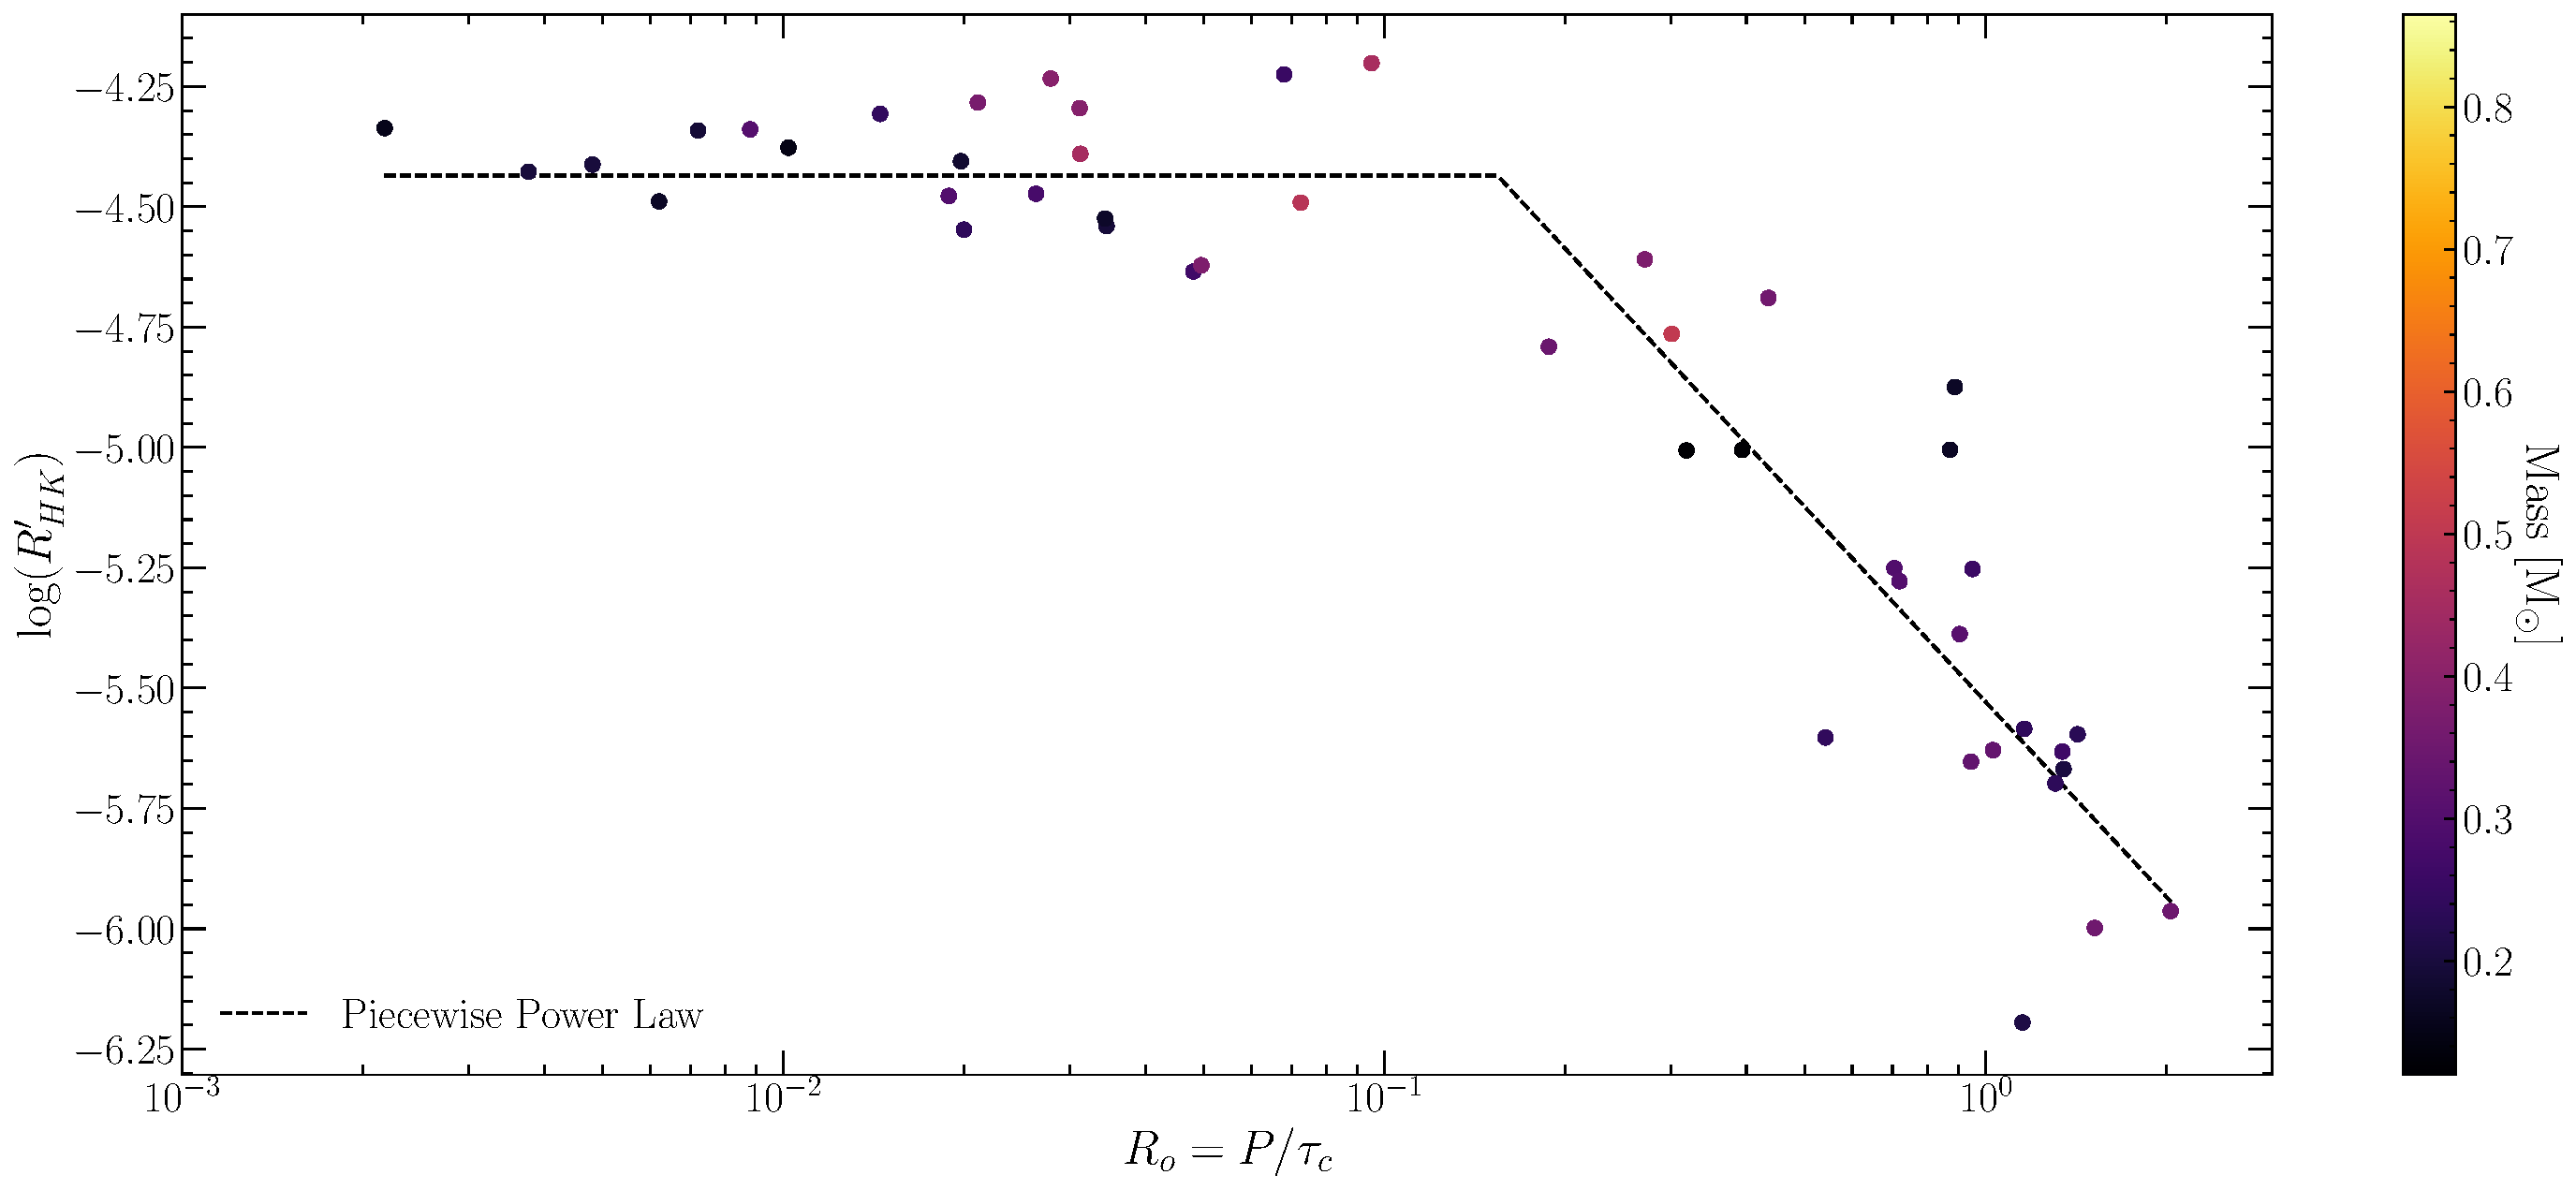
\includegraphics[width=0.9\textwidth]{figures/magActivity/RpHKvsR0_MC_justThisPaper.pdf}
	\caption{Rotation activity relation from this work. The color axis gives
	each stars mass. The dashed line is the best fit to our data set.}
    \label{fig:RpHKvsRossbySelf}
\end{figure*}
\begin{figure*}
    \centering
    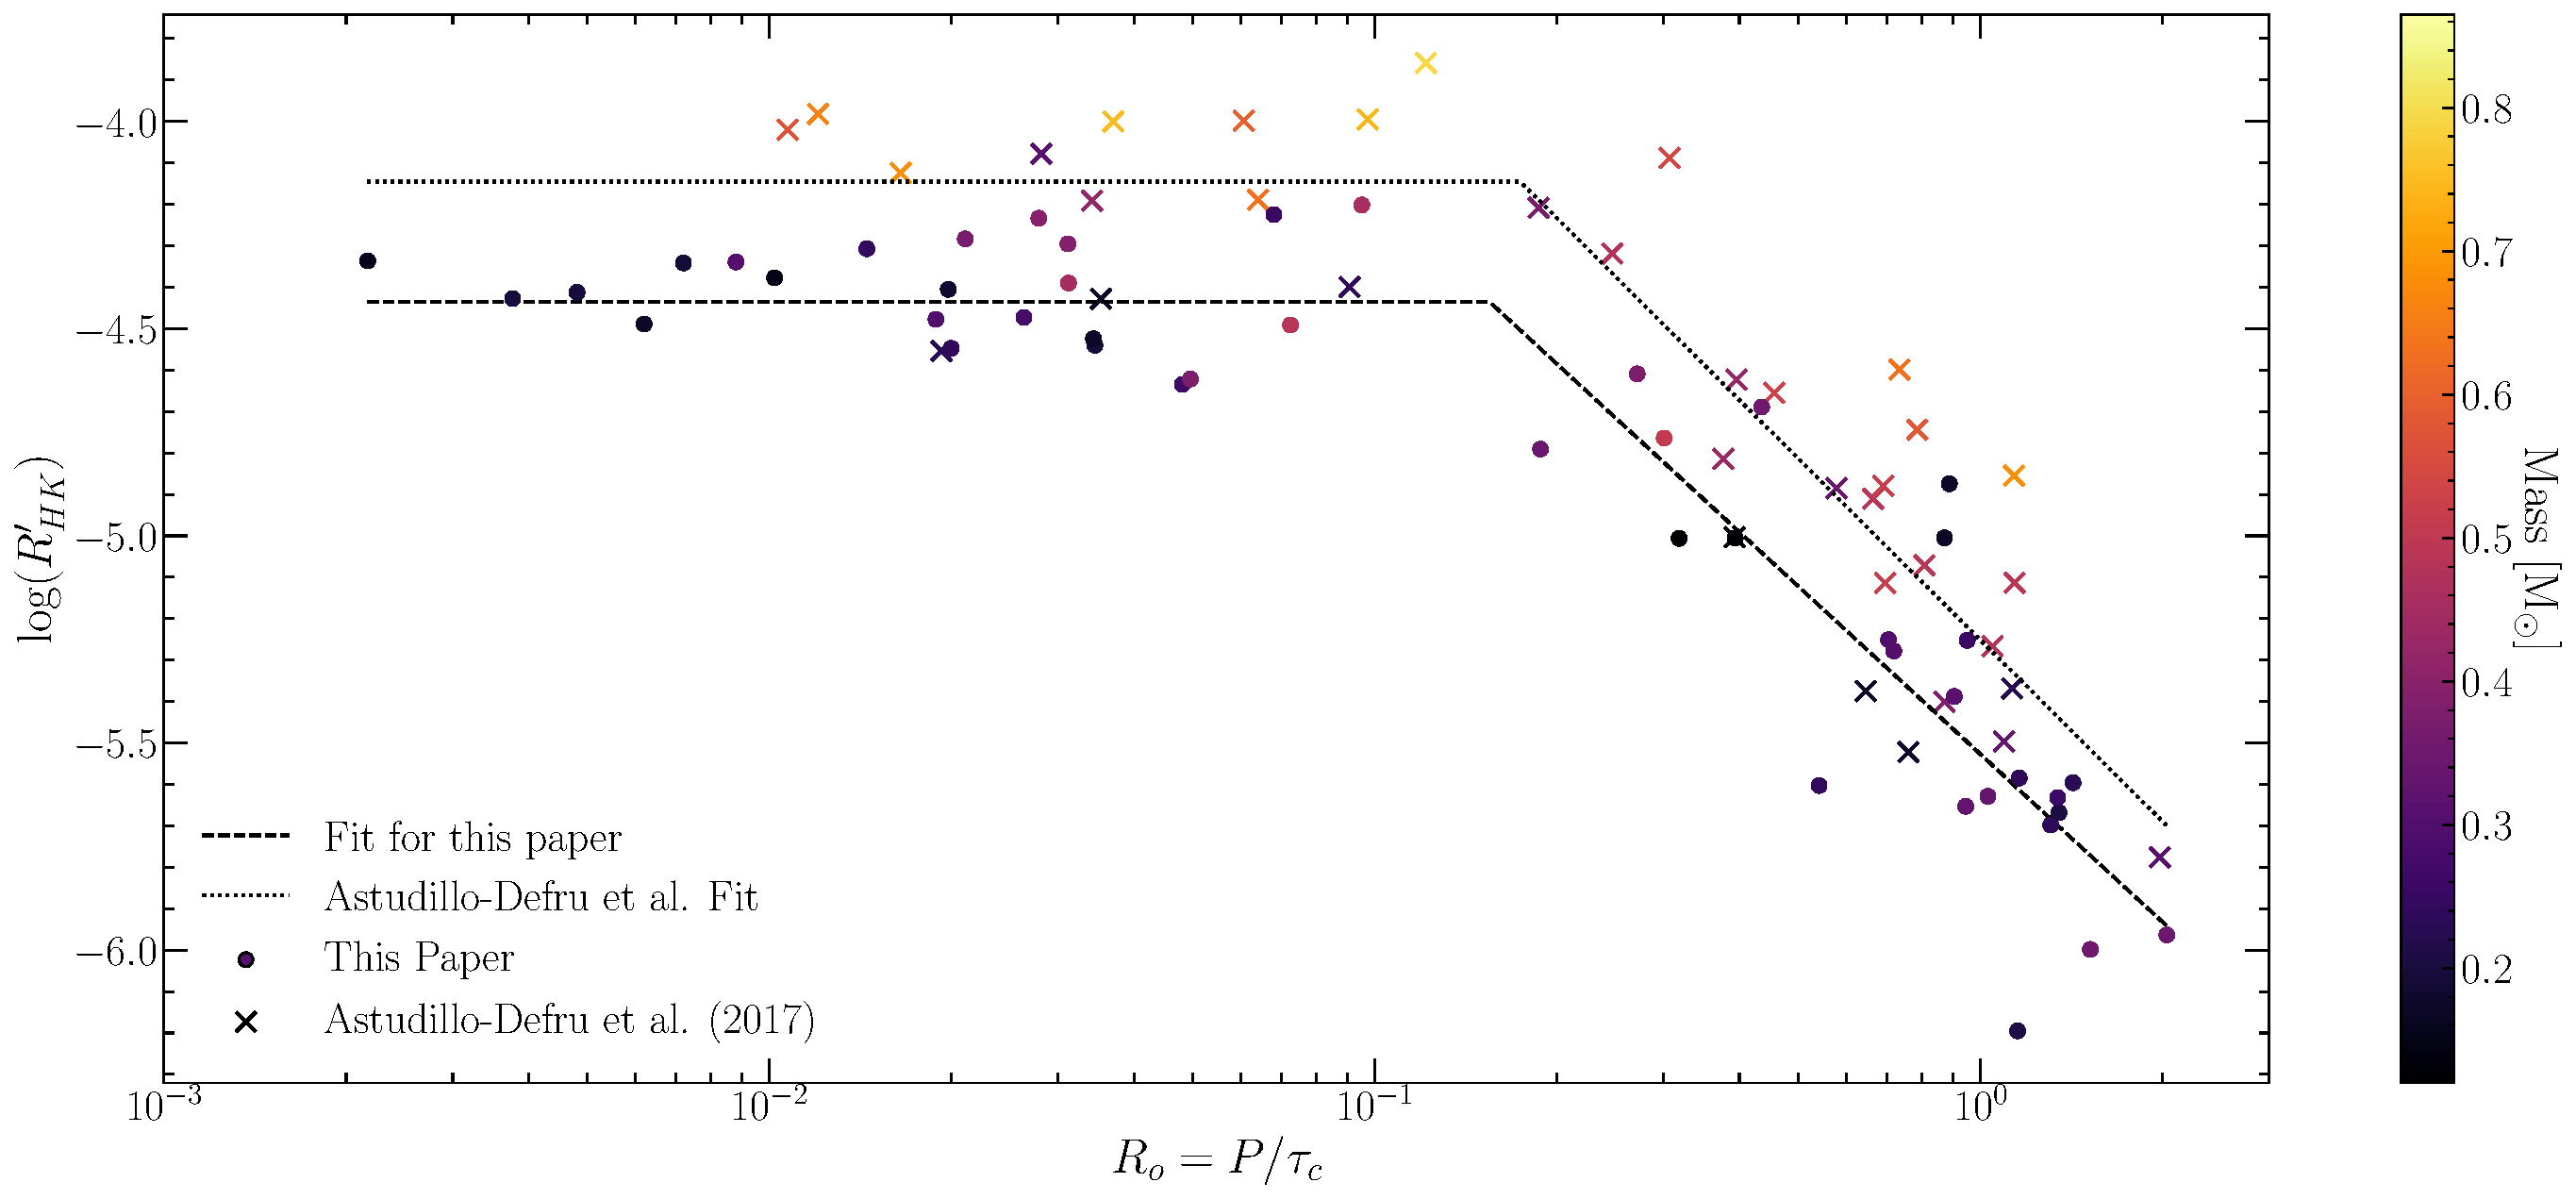
\includegraphics[width=0.9\textwidth]{figures/magActivity/RpHKvsR0_MC.pdf}
	\caption{Rotation activity relation for both our work and \citet{Def17}.
	The dotted line is the best fit to the re-derived rotation-activity
	relation from \citet{Def17}.  Note that targets from \citet{Def17} are
	systematically higher than targets presented here as a consequence of the
	range in mass probed by the samples.}
    \label{fig:RpHKvsRossbyDef}
\end{figure*}
\begin{figure*}
    \centering
    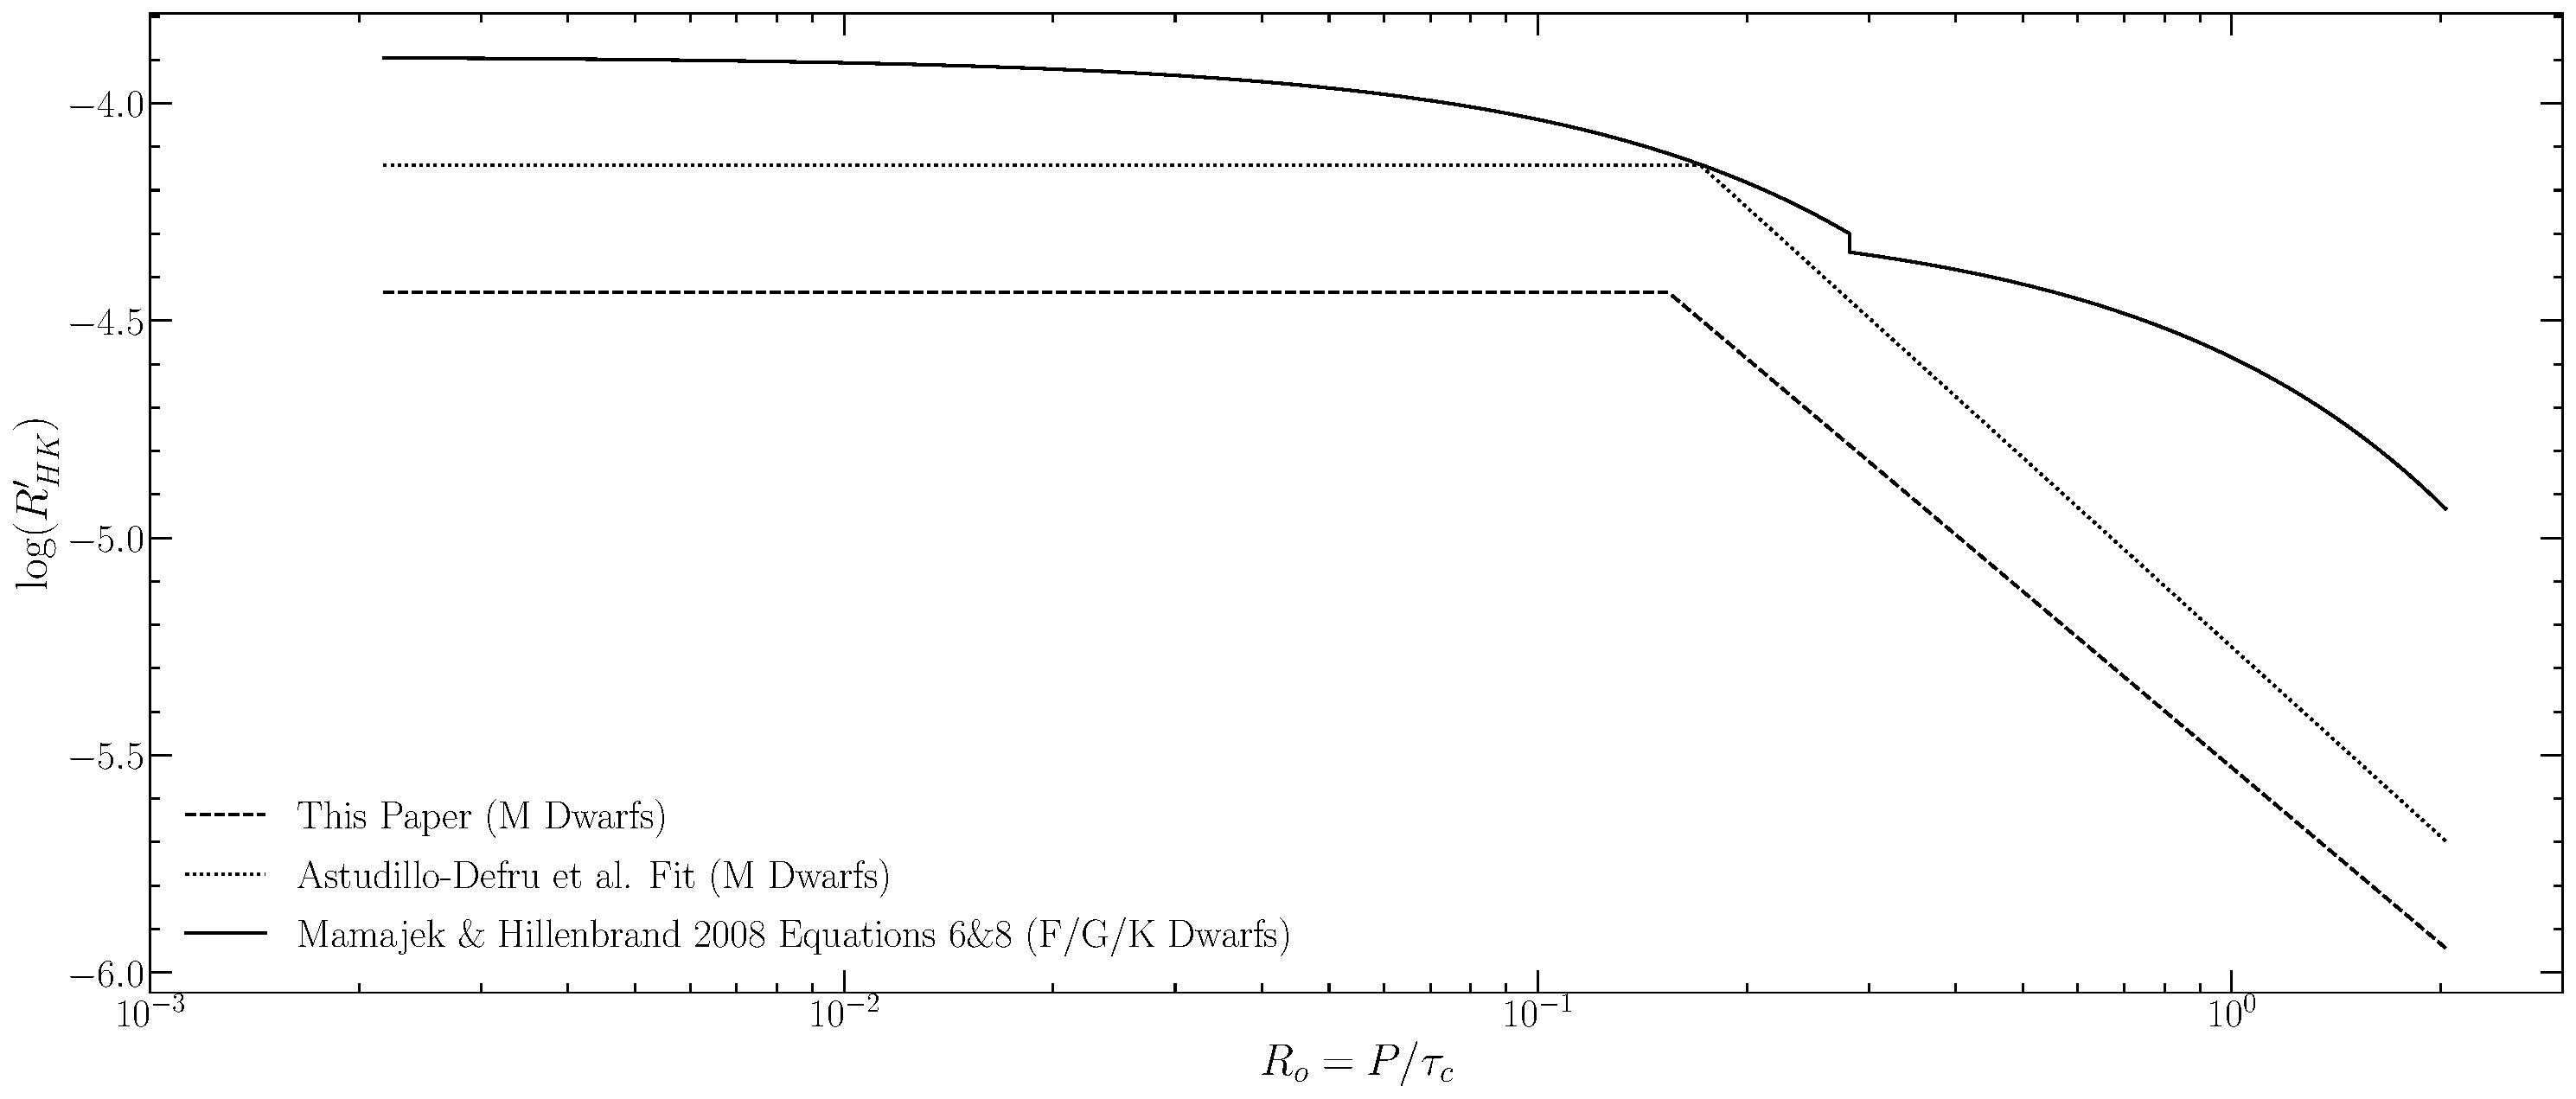
\includegraphics[width=0.9\textwidth]{figures/magActivity/RpHKvsR0_MC_fits.pdf}
	\caption{Derived rotation-activity curves from this work, \citet{Def17} and
	\citet{Mamajek2008}. Note both that \citet{Mamajek2008} focuses their work
	on earlier spectral classes and fits the rotation activity relation in
	linear space.}
    \label{fig:RpHKvsRossbyFits}
\end{figure*}

We find best fit parameters with one $\sigma$ errors:
\begin{itemize}
    \item $k = -1.347\pm 0.203$
    \item $Ro_{s} =  0.155\pm0.045$
    \item $\log(R_{s}) = -4.436\pm0.048$

\end{itemize}
A comparison of the rotation activity derived in this work to those
from both \citet{Def17} and \citet{Mamajek2008} is presented in Figure
\ref{fig:RpHKvsRossbyFits}. For the 6 targets which do not have measured
rotational periods we include an estimate of $Ro$ and $p_{rot}$ in the machine
readable version of Table \ref{tab:finalData}. The convective overturn
timescale for one of these 6 targets (2MASS J13464102-5830117) can not be
inferred via Equation \ref{eqn:convectiveOverturn} as it lacks a V-K color
measurement. Instead, we infer $\tau_{c}$ via \citet{Wri18} Equation 6 (this
paper Equation \ref{eqn:ConvectiveOverturnTimeMass}) using mass. Similar to our
manner of inferring $\tau_{c}$ via color, when inferring $\tau_c$ via mass, we
adopt the larger of the two antisymmetric errors from \citet{Wri18}.

\begin{equation}\label{eqn:ConvectiveOverturnTimeMass}
	\log_{10}(\tau_{c}) = 2.33\pm0.06 - 1.5\pm0.21\left(M/M_{\odot}\right) + 0.31\pm0.17\left(M/M_{\odot}\right)^{2}
\end{equation}

Note that $R'_{HK}$ for one of six of these targets (2MASS
J15165576-0037116) is consistent to within 1$\sigma$ of the saturated value;
therefore, the reported $Ro$ for this target should only be taken as an upper
bound. The remaining five targets have measured $R'_{HK}$ values consistent
with the unsaturated regime. Estimated periods are consistent with previous
constraints. Of the six stars, two were listed as non-detections in
\citet{Newton2018}, and the remaining four as uncertain (possible) detections.
Of the four classed as uncertain, 2MASS 12384914-3822527 and 2MASS
19204795-4533283 have candidate periods $>100$ days and non-detections of
H-alpha emission \citep{Hawley96}. These two stars and the two non-detections
have Ca II H\&K activity levels suggesting very long periods. 2MASS
13464102-5830117 has a candidate period of 45 days, and 2MASS 15165576-0037116
of 0.8 days, both consistent with their higher levels of Ca II H\&K emission.

As a test of the proposed weak correlation between activity and rotation in the
``saturated'' regime seen in some works \citep{Mamajek2008,
Reiners2014, Leh20, Med20} --- though not in others \citep{Wri11, Nunez2015,
Newton2017} ---   we fit a second model whose power law index is allowed to
vary at $Ro < Ro_{s}$. We find a saturated regime power law index of
$-0.052\pm0.117$, consistent with 0 to within 1$\sigma$. Moreover,
all other parameter for this model are consistent to within one $\sigma$ of the
nominal  parameters for the model where the index is constrained to 0 below
$Ro=Ro_{s}$. We can constrain the slope in the saturated
regime to be between -0.363 and 0.259 at the $3\sigma$ confidence level.
Ultimately, we adopt the most standard activity interpretation, a
fully-saturated regime at $Ro < Ro_{s}$. 

We investigate whether our lack of detection of a slope for $Ro <
Ro_{s}$ is due to the limited number of observations in that region when
compared to other works \citep[e.g.][93 targets $Ro < Ro_{s}$]{Med20} through
injection and recovery tests. We inject, fake, rotation-activity measurements
into the saturated regime with an a priori slope of -0.13 --- the same as in
\citeauthor{Med20}. These fake data are given a standard deviation equal to the
standard deviation of our residuals ($12\%$). We perform the same MCMC model
fitting to this new data set as was done with the original data set multiple
times, each with progressively more injected data, until we can detect the
injected slope to the three sigma confidence level. Ultimately, we need more
than 65 data points --- 43 more than we observed in the saturated regime --- to
consistently recover this slope. Therefore, given the spread of our data we
cannot detect slopes on the order of what has previously been reported in the
literature.

We observe a gap in rotational period over a comparable range to the
one presented in \citet{Newton2016} Figure 2. Namely, that M-dwarfs are
preferentially observed as either fast or slow rotators, with a seeming lack of
stars existing at mid rotational periods. This period gap manifests in the
Rossby Number and can be seen in Figure \ref{fig:RpHKvsRossbyDef} as a lack of
our targets near to the knee-point in the fit. This period gap likely
corresponds to that seen by \citet{Browning2010}, who found a paucity of M
dwarfs at intermediate activity levels in Ca II H\&K and note the similarity to
the Vaughn-Preston gap established in higher mass stars \citep{vaughan1980}.
\citet{Magaudda2020} also identify a double-gap in x-ray activity for stars in
the unsaturated regime; it is not clear that the gap we see is related. As a
consequence of this period gap, there exists a degeneracy in our data
between moving the knee-point and allowing the activity level to vary in the
saturated regime.  In the following, we adopt the model of a fully saturated
regime.

We wish to compare our best fit parameters to those derived in \citet{Def17};
however, the authors of that paper do not fit the knee-point of the
rotation-activity relation. They select the canonical value for the rotational
period separating the saturated regime from the unsaturated regime ($P_{rot,s}
= 10$ days) and use a fixed convective overturn timescale ($\tau_{c} = 70$
days). To make our comparison more meaningful we use the $P_{rot}$ and $V-K$
colors presented in \citet{Def17} to re-derive $Ro$ values using $\tau_{c}$
\citep{Wri18}. Doing this for all targets presented in \citet{Def17} Table 3
and fitting the same piecewise power law as before, we find best fit parameters
of $Ro_{s} = 0.17\pm0.04$, $\log(R_{s}) = -4.140\pm0.067$, and
$k=-1.43\pm0.21$. Compared to the best fit parameters for our data, $Ro_{s}$
and the unsaturated regime's index, $k$, are consistent to within one sigma,
while the saturated value, $R_{s}$, differs. 

The mass ranges of our respective samples explain the differences in saturation
values between our work and that of \citet{Def17}. Our work focuses on
mid-to-late M-dwarfs and includes no stars above a mass of $0.5$ M$_{\odot}$
(Figure \ref{fig:massDistribution}).  The strength of Ca II H\&K
emission is known to decrease as stellar mass decreases \citep{Schrijver1987,
Rauscher2006, Hou17}. As \citet{Rauscher2006} note, this is the opposite as the
trend seen in H-alpha; the latter primarily reflects the increasing length of
time that lower M dwarfs remain active and rapidly rotating \citep{West2015,
Newton2016}.

A mass dependence can be seen in Figure 10 in \citet{Def17}, consistent
with expectations from the literature. If we clip the data from \citet{Def17}
Table 3 to the same mass range as our data-set ($M_{*} < 0.5M_{\odot}$) and fit
the same function as above, we find that all best fit parameters are consistent
to within one sigma between the two data-sets. 

\begin{figure}
    \centering
    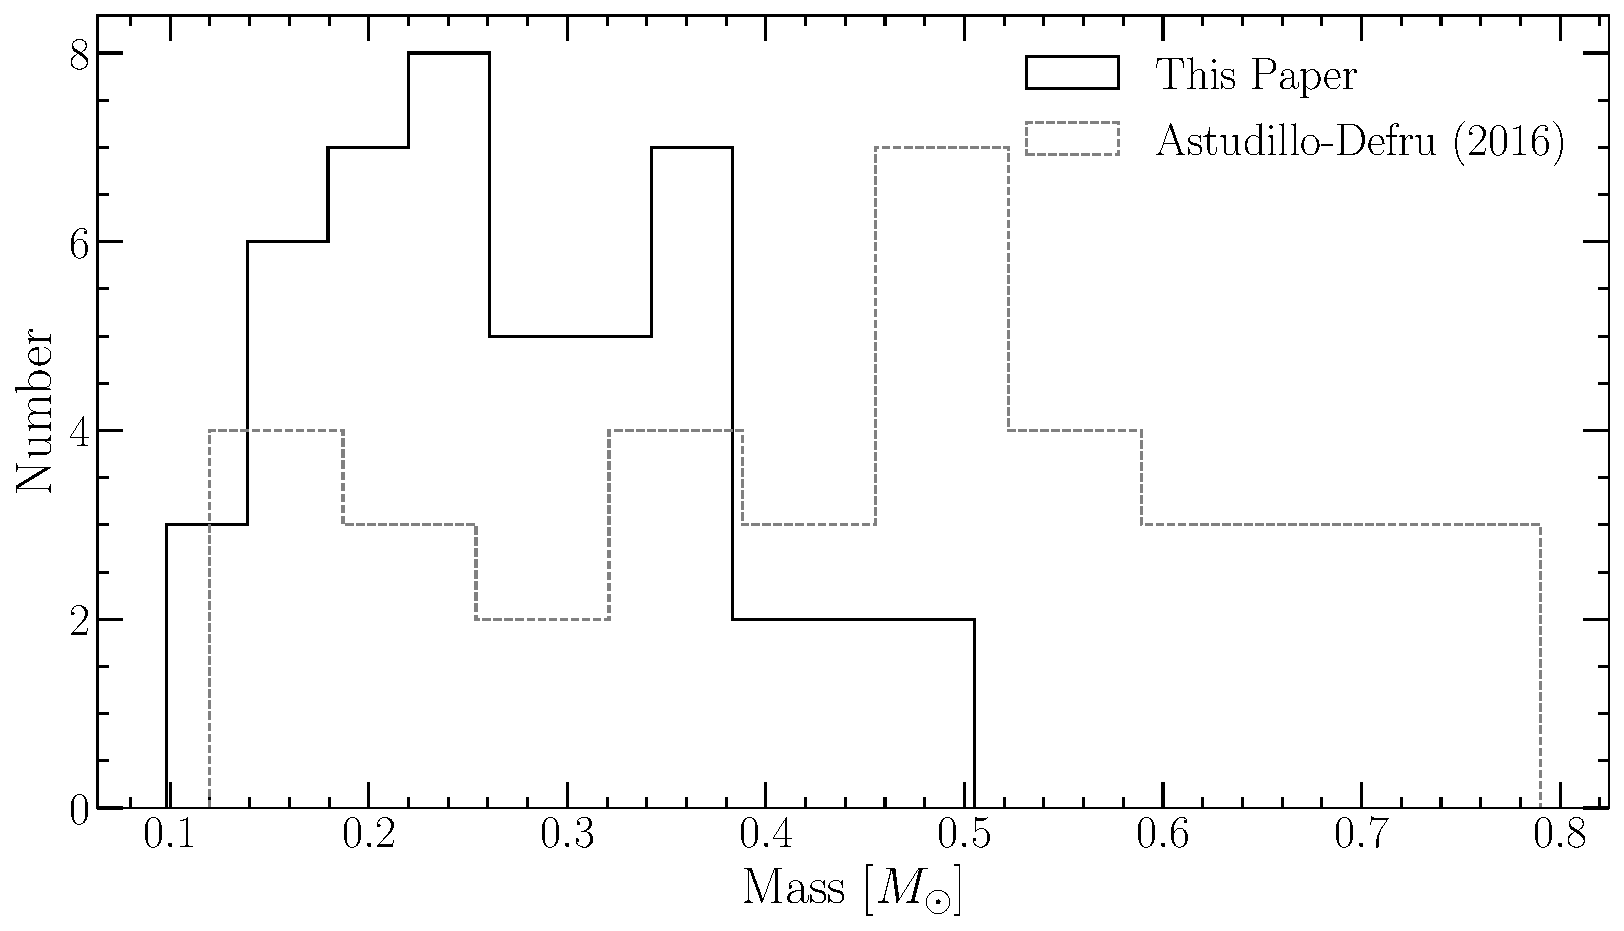
\includegraphics[width=0.85\textwidth]{figures/magActivity/B2020vsAD2016_Masses.pdf}
	\caption{Distribution of masses between our sample and the sample presented
	in \citet{Def17}. Note how the two studies have approximately the same
	sample sizes; however, our sample is more tightly concentrated at lower
	masses \textbackslash later spectral classes.}
    \label{fig:massDistribution}
\end{figure}

We also compare our best fit $Ro_{s}$ to both those derived in
\citet{Newton2017} using $H_{\alpha}$ as an activity measure and those derived
in \citep{ Wri18, Magaudda2020} using $L_{X}/L_{bol}$ as an activity measure.
Works using $L_{X}/L_{bol}$ identify a similar, yet not consistent to within
one sigma result for $Ro_{s}$; while, the value of $k$ we find here is
consistent between all four works. Therefore, we find similar results not only
to other work using the same activity tracer, but also a power-law slope that
is consistent with work using different tracers. 





\chapter{Jao Gap connection to Magnatism}
\section{Introduction}\label{sec:Intro}
Globular clusters (GCs) are among the oldest observable objects in the universe
\citep{Pen11}. They are characterized by high densities with typical half-light
radii of $\le$10 pc \citep{Vanderburg2010}, and typical masses ranging from
$10^{4}$--$10^{5}$ M$_{\odot}$ \citep{Bro06} --- though some GCs are
significantly larger than these typical values \citep[e.g. $\omega$ Cen,
][]{Richer1991}. GCs provide a unique way to probe stellar evolution
\citep{Bau03}, galaxy formation models \citep{Boy18,Kra05}, and dark matter
halo structure \citep{Hud18}.

The traditional view of Globular Clusters was that they consisted of a single
stellar population (SSP, in some publications this is referred to as a Simple
Stellar Population). This view was supported by spectroscopically uniform heavy
element abundances \citep{Carretta2010, Bastian2018} across most clusters (M54
and $\omega$Cen are notable exceptions, see \citet{Marino2015} for further
details), and the lack of evidence for multiple stellar populations (MPs) in
past color-magnitude diagrams of GCs \citep[i.e.][]{Sandage1953, Alcaino1975}.
However, over the last 40 years non-trivial star-to-star light-element
abundance variations have been observed \citep[i.e.][]{Smith1987} and, in the
last two decades, it has been definitively shown that most if not all Milky Way
GCs have MPs \citep{Gratton2004, Gratton2012, Piotto2015}. The lack of
photometric evidence for MPs prior to the 2000, can be attributed to the more
narrow color bands available, until very recently, to ground based photometric
surveys \citep{Milone2017}.

The prevalence of multiple populations in GCs is so distinct that the proposed
definitions for what constitutes a globular cluster now often center the
existence of MPs \citep[e.g.][]{Carretta2010}. Whereas, people have have often
tried to categorized objects as GCs through relations between half-light
radius, density, and surface brightness profile, in fact many objects which are
generally thought of as GCs don't cleanly fit into these cuts
\citep{Peebles1968, Brown1991, Brown1995, Bekki2002}. Consequently,
\citet{Carretta2010} proposed a definition of GC based on observed chemical
inhomogeneities in their stellar populations. The modern understanding of GCs
then is not simply one of a dense cluster of stars that may have chemical
inhomogeneities and multiple populations; rather, it is one where those
chemical inhomogeneities and multiple populations themselves are the defining
element of a GC.

All Milky Way globular clusters studied in detail show populations enriched in
He, N, and Na while also being deplete in O and C
\citep{Piotto2015,Bastian2018}. {\bf Further, studies of Magellenic Cloud
massive clusters have shown that these light element abundance variations exist
in clusters as young as $\sim 2$ Gyr but not in younger clusters
\citep{Martocchia2019} while there is also evidence of nitrogen variability in
the $\sim 1.5$ Gyr old cluster NGC 1783 \citep{Cadelano2022}}.  These light
element abundance patterns also are not strongly correlated with variations in
heavy element abundance, resulting in spectroscopically uniform Fe abundances
between populations \citep[{\bf though recent work indicates that there may be
[Fe/H] variations within the first population, e.g.}][]{Legnardi2022,
Lardo2022} . Further, high-resolution spectral studies reveal anti-correlations
between N-C abundances, Na-O abundances, and potentially Al-Mg
\citep{Sneden1992, Gratton2012}. Typical stellar fusion reactions can deplete
core oxygen; however, the observed abundances of Na, Al, and Mg cannot be
explained by the CNO cycle \citep{Prantzos2007}. Consequently, globular cluster
populations must be formed by some novel means.

Formation channels for these multiple populations remain a point of debate
among astronomers. Most proposed formation channels consist of some older,
more massive, population of stars polluting the pristine cluster media before a
second population forms, now enriched in heavier elements which they themselves could
not have generated \citep[for a detailed review see ][]{Gratton2012}. The four
primary candidates for these polluters are asymptotic giant branch stars
\citep[AGBs,][]{Ventura2001,DErcole2010}, fast rotating massive stars
\citep[FRMSs,][]{Decressin2007}, super massive stars
\citep[SMSs,][]{Denissenkov2014}, and massive interacting binaries
\citep[MIBs,][]{deMink2009, Bastian2018}. 

Hot hydrogen burning (i.e. proton capture), material transport to the surface, and
material ejection into the intra-cluster media are features of each of these
models and consequently they can all be made to {\it qualitatively} agree with
the observed elemental abundances. However, none of the standard models can
currently account for all specific abundances \citep{Gratton2012}. AGB and FRMS
models are the most promising; however, both models have difficulty reproducing
severe O depletion \citep{Ventura2009,Decressin2007}. Moreover, AGB and FRMS
models require significant mass loss ($\sim 90\%$) between cluster formation
and the current epoch --- implying that a significant fraction of halo stars
formed in GCs \citep{Renzini2008,DErcole2008,Bastian2015}.

In addition to the light-element anti-correlations observed, it is also known
that second populations are significantly enhanced in Helium
\citep{Piotto2007, Piotto2015, Latour2019}. Depending on the cluster, helium
mass fractions as high as $Y=0.4$ have been inferred \citep[e.g][]{Milone2015}.
However, due to both the relatively high and tight temperature range of partial
ionization for He and the efficiency of gravitational settling in core helium
burning stars, the initial He abundance of globular cluster stars cannot be
observed; consequently, the evidence for enhanced He in GCs originates from
comparison of theoretical stellar isochrones to the observed
color-magnitude-diagrams of globular clusters. Therefore, a careful handling of
chemistry is essential when modeling with the aim of discriminating between
MPs; yet, only a very limited number of GCs have been studied with
chemically self-consistent (structure and atmosphere) isochrones
\citep[e.g.][NGC 6752]{Dotter2015}. 

NGC 2808 is the prototype globular cluster to host Multiple Populations.
Various studies since 2007 have identified that it may host anywhere from 2-5
stellar populations. These populations have been identified both
spectroscopically \citep[i.e.][]{Carretta2004, Carretta2006, Carretta2010,
Gratton2011, Carretta2015, Hong2021} and photometrically
\citep[i.e.][]{Piotto2007, Piotto2015, Milone2015, Milone2017, Pasquato2019}.
Note that recent work \citep{Valle2022} calls into question the statistical
significance of the detections of more than 2 populations in the spectroscopic
data. Here we present new, chemically self-consistent modeling of the
photometry of the two extreme populations of NGC 2808 identified by
\citet{Milone2015}, populations A and E. {\bf We do not consider populations B,
C, or D identified in \citet{Milone2015} as the purpose of this work is to
identify if chemically self-consistent modelling results in a statisically
signifigant deviation in the infered helium abundance when compared to non
chemically self-consistent models. Use of the two populations in the NGC 2808
with the highest identified difference between their helium populations is
sufficent for to answer this question.}  We use archival photometry from the
Hubble UV Globular Cluster Survey (HUGS) \citep{Piotto2015, Milone2017} in the
F275W and F814W passbands to characterize multiple populations in NGC 2808
\citep{Milone2015, Milone2015b} (This data is avalible at MAST: \href{https://archive.stsci.edu/doi/resolve/resolve.html?doi=10.17909/T9810F}{10.17909/T9810F}). Additionally, we present a
likelihood analysis of the photometric data of NGC 2808 to determine the number
of populations present in the cluster.



\section{Correlation}\label{sec:results}
Using Ca II H\&K emission data from \citet{Boudreaux2022} and
\citet{Perdelwitz2021} (quantified using the $R_{HK}$ metric) we investigate
the correlation between the Jao Gap magnitude and stellar magnetic activity. We
are more statistically limited here than past authors have been due to
the requirement for high resolution spectroscopic data when measuring Calcium
emission; however, this is balanced by the apparent stronger correlation between
Calcium emission and the Jao gap when compared to H$\alpha$ emission. 

The merged dataset is presented in Figure \ref{fig:mergedData}. There is a
visual discontinuity just below the Jao Gap magnitude; however, this
manifests as an increase in the spread of the emission measurements rather than
a change in the mean value. In order to quantify the significance of this
discontinuity we measure the false alarm probability of the change in standard
deviation.

\begin{figure}
  \centering
  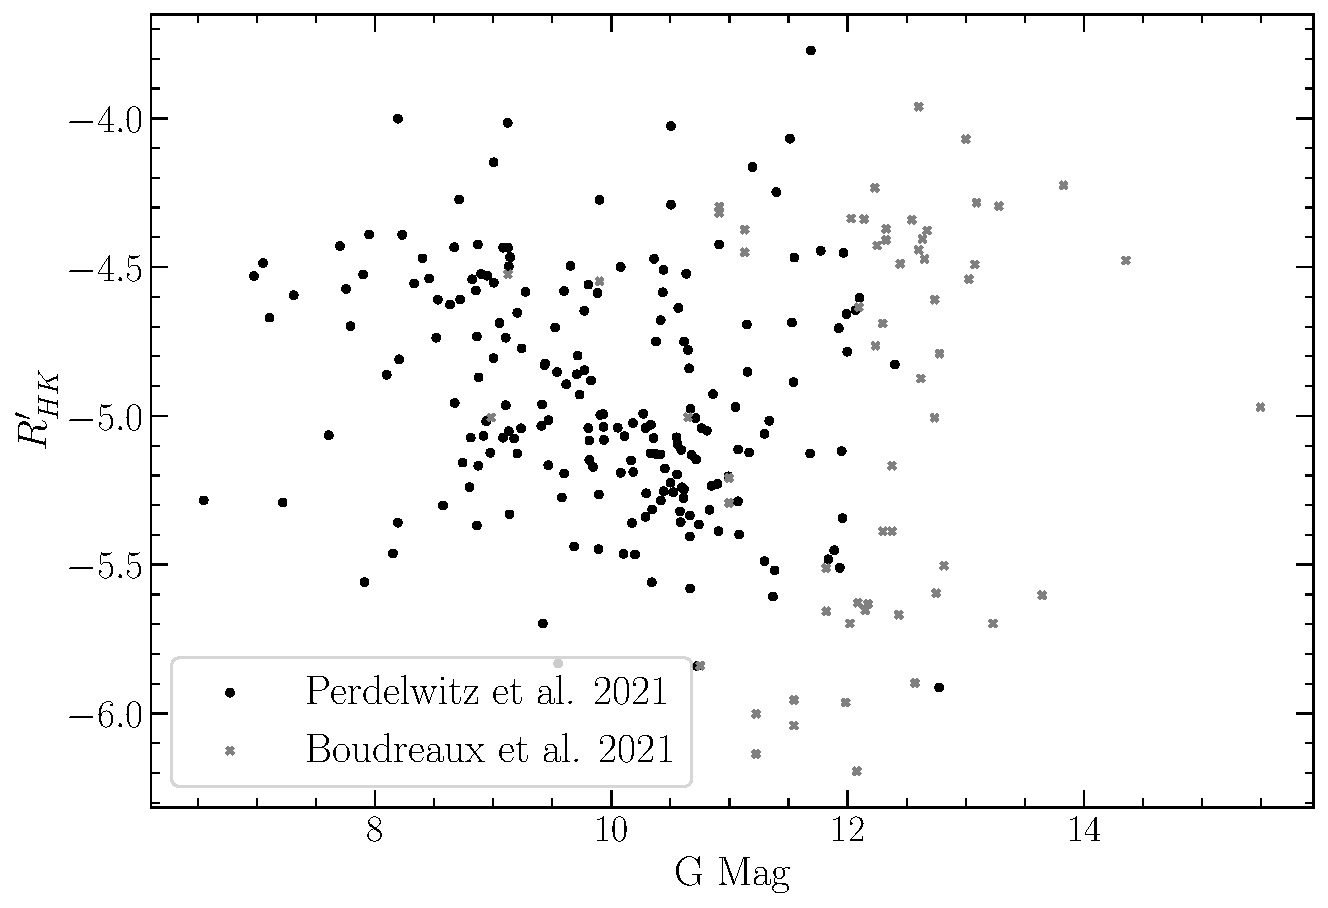
\includegraphics[width=0.45\textwidth]{figures/jaoMagActivity/Combined.pdf}
  \caption{Merged Dataset from \citet{Boudreaux2022, Perdelwitz2021}. Note the
  increase in the spread of $R'_{HK}$ around the Jao Gap Magnitude.}
  \label{fig:mergedData}
\end{figure}

First we split the merged dataset into bins with a width of 0.5 mag. In each bin we
measure the standard deviation about the mean of the data. The results of this
are shown in Figure \ref{fig:deviation}. In order to measure the false alarm
probability of this discontinuity we first resample the merged calcium
emission data based on the associated uncertainties for each datum as
presented in their respective publications. Then, for each of these ``resample
trials'' we measure the probability that a change in the standard deviation of
the size seen would happen purely due to noise. Results of this test are show in
in Figure \ref{fig:dist}. 

\begin{figure}
  \centering
  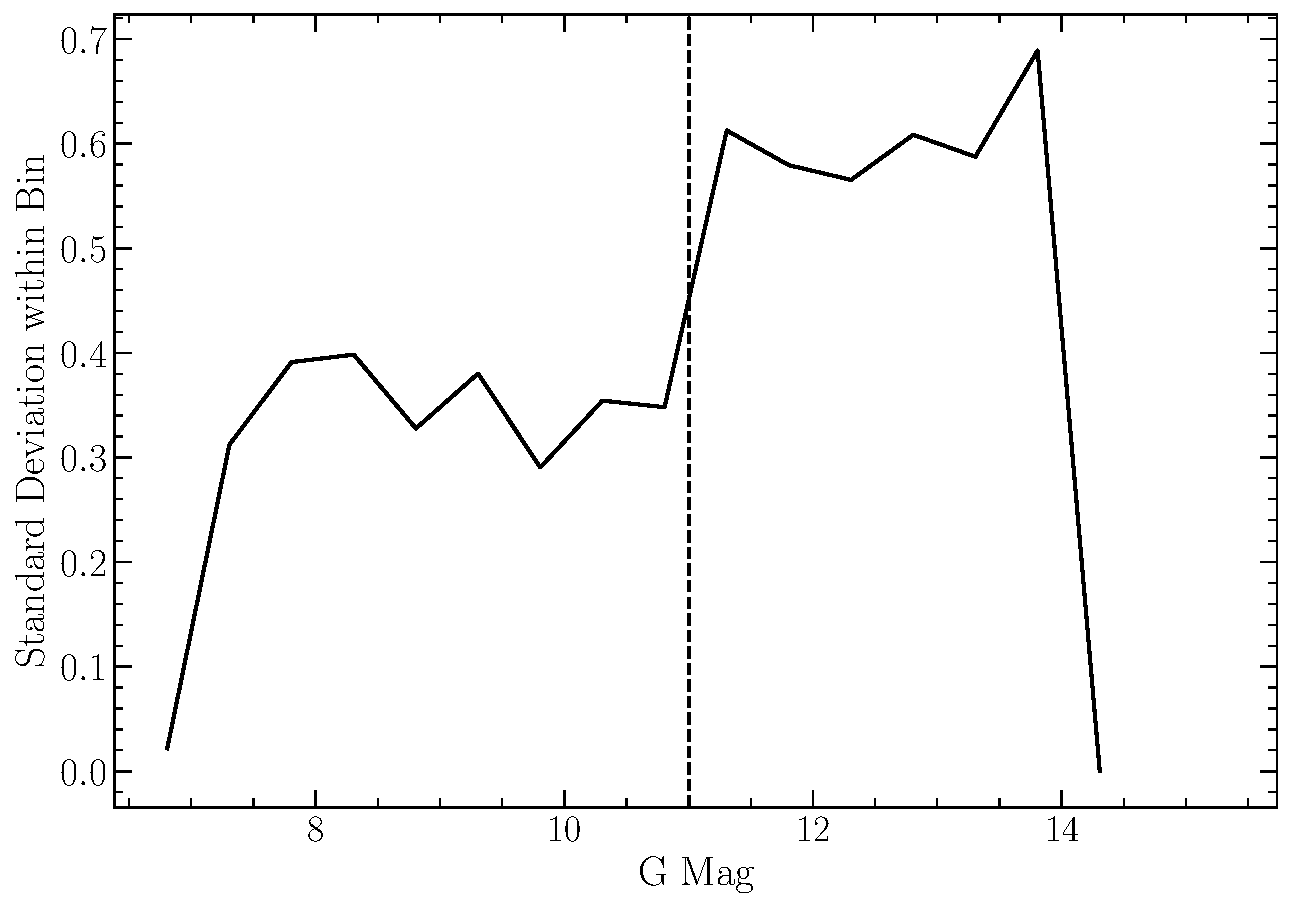
\includegraphics[width=0.45\textwidth]{figures/jaoMagActivity/Deviation.pdf}
  \caption{Standard deviation of Calcium emission data within each bin. Note
  the discontinuity near the Jao Gap Magnitude.}
  \label{fig:deviation}
\end{figure}

\begin{figure}
  \centering
  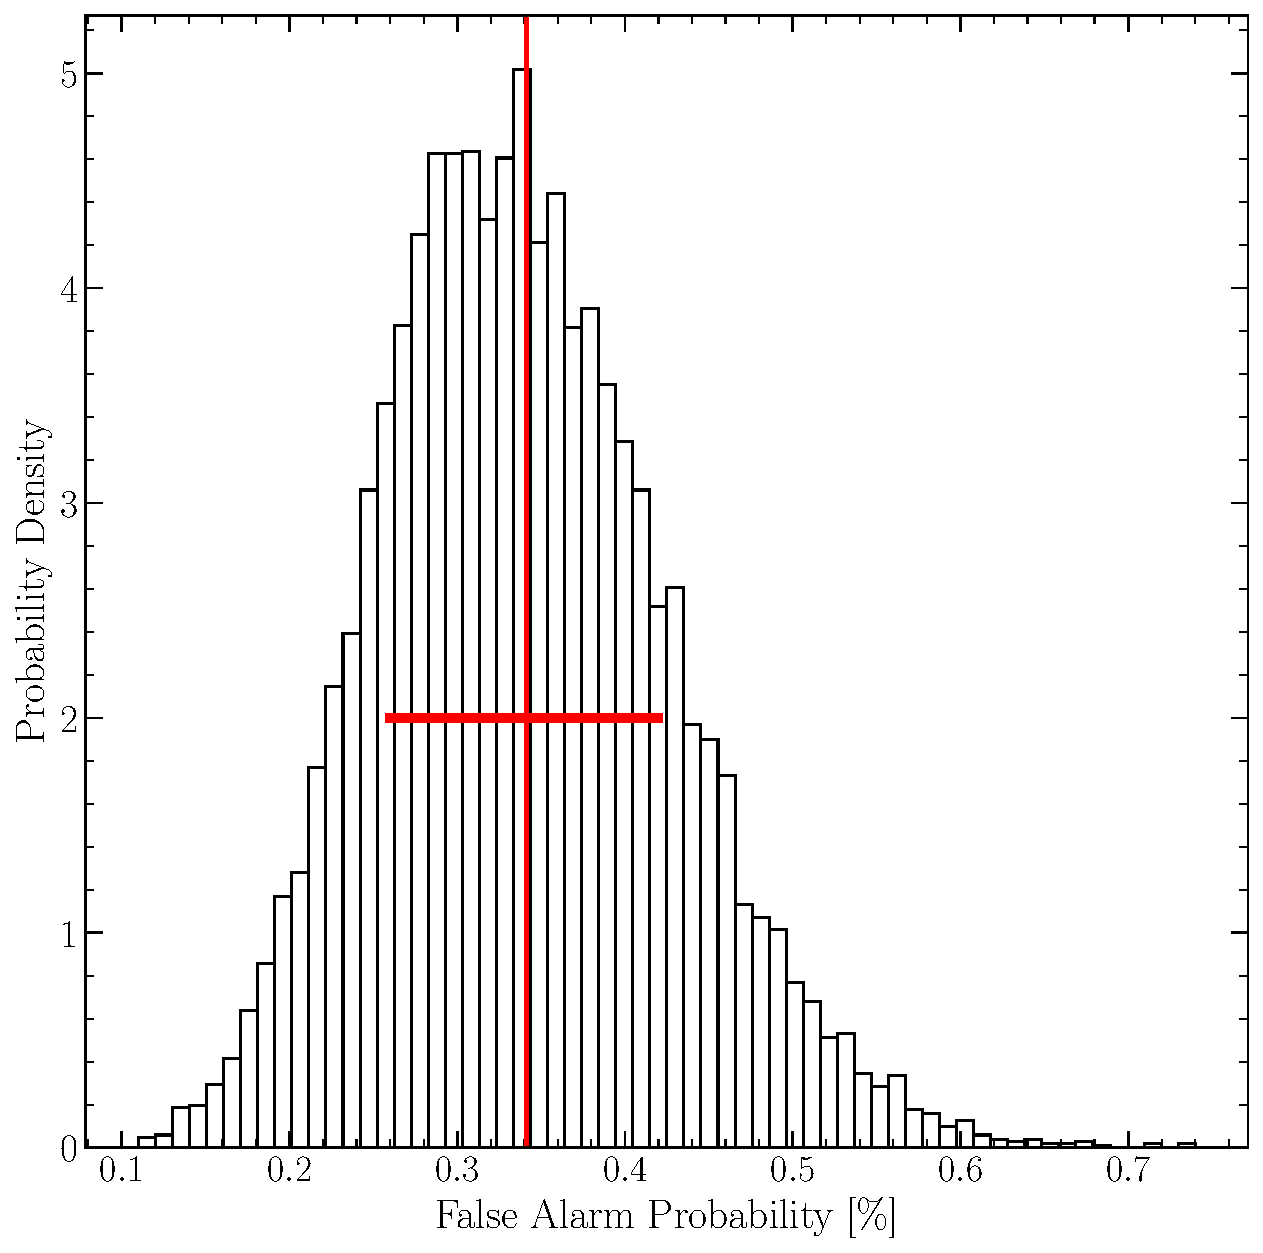
\includegraphics[width=0.45\textwidth]{figures/jaoMagActivity/fpDist.pdf}
  \caption{Probability distribution of the false alarm probability for the
  discontinuity seen in Figure \ref{fig:deviation}. The mean of this
  distribution is $0.341\%\pm^{0.08}_{0.08}$.}
  \label{fig:dist}
\end{figure}

This rapid increase star-to-star variability would only arise due purely to
noise $0.3\pm0.08$ percent of the time and is therefore likely either a true
effect or an alias of some sample bias. {\color{red} COME BACK TO HERE TO FLUSH
OUT SAMPLE BIAS SECTION.}

If the observed increase in variability is not due to a sample bias and rather
is a physically driven effect then there is an obvious similarity between these
findings and those of \citep{Jao2023}. Specifically we find a increase in
variability just below the magnitude of the gap. Moreover, this variability
increase is primarily driven by an increase in the number of low activity stars
(as opposed to an increase in the number of high activity stars). We can
further investigate the observed change in variability for only low activity
stars by filtering out those stars at or above the saturated threshold for
magnetic activity. \citet{Boudreaux2022} identify $\log(R'_{HK}) = -4.436$ as
the saturation threshold. We adopt this value and filter out all stars where
$\log(R'_{HK}) \geq -4.436$. Applying the same analysis to this reduced dataset
as was done to the full dataset we still find a discontinuity at the same
location (Figure \ref{fig:reduced}). This discontinuity is of a smaller
magnitude and consequently is more likely to be due purely to noise, with a
$7\pm0.2$ percent false alarm probability. This false alarm probability is
however only concerned with the first point after the jump in variability. If
we consider the false alarm probability of the entire high variability region
then the probability that the high variability region is due purely to noise
drops to $1.4\pm0.04$ percent.

\begin{figure}
  \centering
  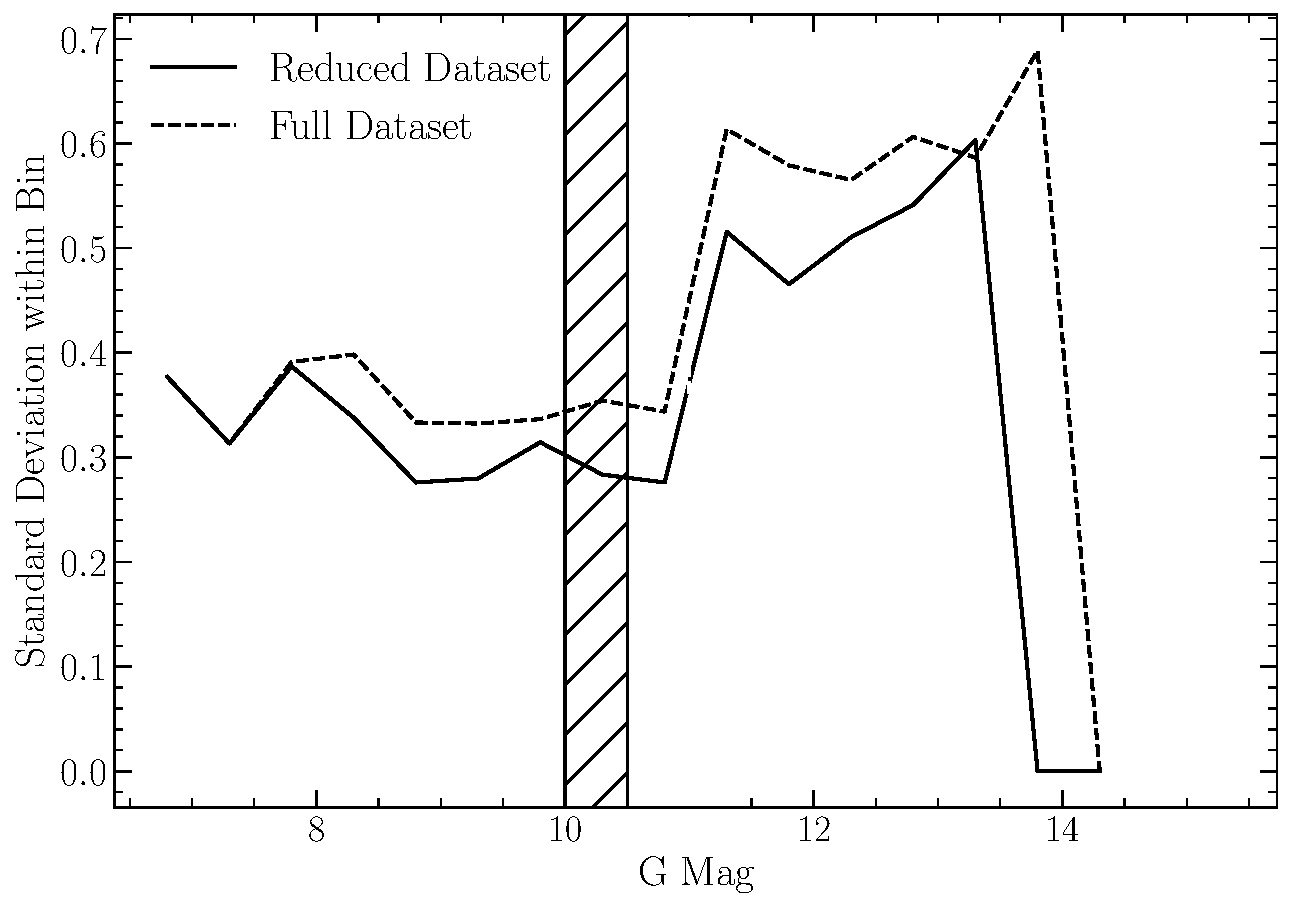
\includegraphics[width=0.45\textwidth]{figures/jaoMagActivity/ReducedDeviation.pdf}
  \caption{Spread in the magnetic activity metric for the merged sample with
  any stars $\log(R'_{HK}) > -4.436$ filtered out.}
  \label{fig:reduced}
\end{figure}

We observe a strong, likely statistically significant, discontinuity in the
star-to-star variability of Ca II K \& K emission just below the magnitude
of the Jao Gap. However, modeling is required to determine if this discontinuity
may be due to the same underlying physics.

While the observed increase in variability seen here does not seem to be
coincident with the Jao Gap --- instead appearing to be approximately 0.5 mag
fainter, in agreement with what is observed in \citet{Jao2023} --- a number of
complicating factors prevent us from falsifying that the these two features are
not coincident. \citeauthor{Jao2023} find, similar to the results presented
here, that the paucity of $H\alpha$ emission originates just below the gap.
Moreover, we use a 0.5 magnitude bin size when measuring the star-to-star
variability which injects error into the positioning of any feature in
magnitude space. We can quantify the degree of uncertainty the magnitude bin
choice injects by conducting Monte Carlo trials where bins are randomly shifted
redder or bluer. We conduct 10,000 trials where each trial involves sampling a
random shift to the bin start location from a normal distribution with a
standard deviation of 1 magnitude. For each trial we identify the discontinuity
location as the maximum value of the gradient of the standard deviation
(effectively this is just the derivative of \ref{fig:reduced}). Some trials
result in the maximal value lying at the 0th index of the magnitude array due
to edge effects, these trials are rejected (and account for 11\% of the
trials). The uncertainty in the identified magnitude of the discontinuity due
to the selected start point of the magnitude bins reveals a $1\sigma = \pm$0.32
magnitude uncertainty in the location of the discontinuity (Figure
\ref{fig:GapLocationMC}). Finally, all previous studies of the M dwarf gap
\citep{Jao2018, Feiden2022, Mansfield2021, Boudreaux2022, Jao2023} demonstrate
that the gap has a color dependency, shifting to fainter magnitudes as the
population reddens and consequently an exact magnitude range is ill-defined.
Therefore we cannot falsify the model that the discontinuity in star-to-star activity
variability is coincident with the Jao Gap magnitude.

\begin{figure}
  \centering
  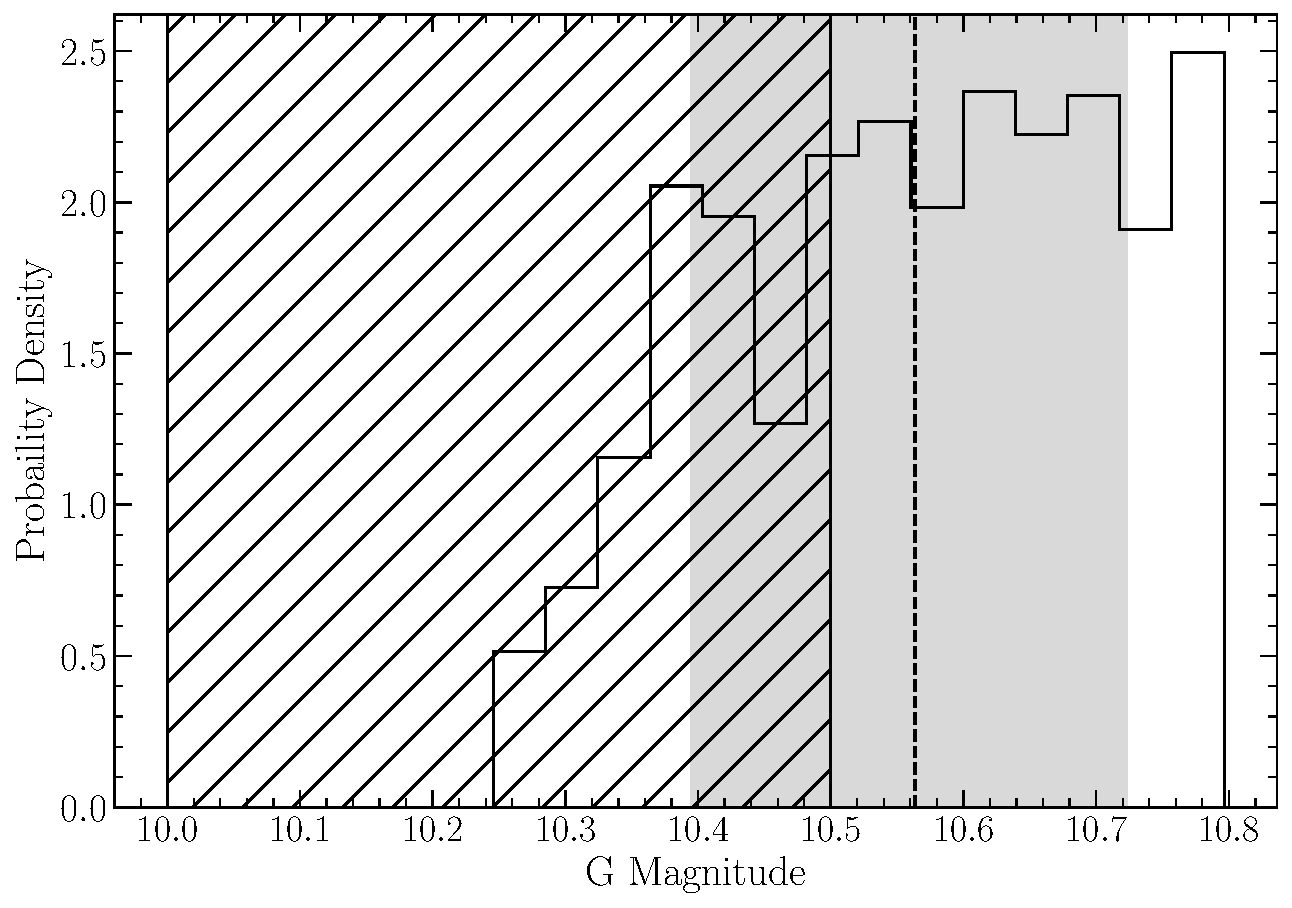
\includegraphics[width=0.45\textwidth]{figures/jaoMagActivity/GapLocationMC.pdf}
  \caption{Probability density distribution of discontinuity location as
  identified in the merged dataset. The dashed line represents the mean of the
  distribution while the shaded region runs from the 16th percentile to the
  84th percentile of the distribution. This distribution was built from 10,000
  independent samples where the discontinuity was identified as the highest
  value in the gradient of the standard deviation.}
  \label{fig:GapLocationMC}
\end{figure}

\subsection{Rotation}
Following the process described in \citet{023AJ....165..192G}, we first put the
dataset through \texttt{stella} \citep{FeinsteinFlare2020,FeinsteinStella2020},
a convolutional neural network that trains a multitude of models, given a
different initial seed, on TESS 2-min cadence. In this case, we also used an
ensemble of 100 models to optimize the gains. \texttt{stella} identifies flares
given a score of 0 to 1, here we use a score of 0.5 and above as flare
identification. Furthermore, we also bin the data from a 2-min to 10-min
cadence using \texttt{lightkurve}'s binning function
\citep{LightkurveCollaborationLightkurve2018,GeertBarentsenKeplerGO2020}. Not
only does this help further reduce any flaring-contribution that might have
been missed by \texttt{stella}\footnote{This is relevant for flares that are
misshapen at the start or break in the dataset due to missing either the
ingress or egress.}, but it also optimizes computational efficiency.
Subsequently, we calculate residuals by subtracting the model from the data,
retaining data with residuals smaller than 4 times the root-mean-square.

As M dwarfs often exhibit non-sinusoidal and quasi-periodic rotational
variability, we employ Gaussian processes for modeling based on
\citet{AngusInferring2018} for the subset of M Dwarfs with no fiducial periods.
The \texttt{starspot} \ package is adapted for light curve analysis
\citep{AngusRuthAngus2021,https://doi.org/10.5281/zenodo.7697238} and
accessible at (HAVEN'T DONE IT YET-AYLIN). Our Gaussian process kernel function
incorporates two stochastically-driven simple harmonic oscillators,
representing primary ($P_\textrm{rot}$) and secondary ($P_\textrm{rot}/2$)
rotation modes. First, we implement the Lomb-Scargle periodogram within
\texttt{starpot} to initially estimate the period. After which, we create a
maximum a posteriori (MAP) fit using \texttt{starspot} to generate a model for
stellar rotation. To obtain the posterior of the stellar rotation model, we use
Markov Chain Monte Carlo (MCMC) sampling using the \texttt{pymc3} package
\citep{SalvatierProbabilistic2016} within our adapted \texttt{starspot}
version. 

ANALYSIS PART YET TO BE DETERMINED.

\subsection{Limitations}
There are two primary limitation of our dataset. First, we only have
{\color{red}232 stars} in our dataset limiting the statistical power of our
analysis. This is primarily due to the relative difficulty of obtaining Ca II
H\&K measurements compared to obtaining $H\alpha$ measurements. Reliable
measurements require both high spectral resolutions ({\color{red} R $\sim$
XXXXXX}) and a comparatively blue wavelength range \footnote{wrt. too what many
spectrographs cover. There is no unified resource listing currently
commissioned spectrographs; however, it is somewhat hard to source glass which
transmits well at H\&K wavelengths limiting the lower wavelength of most
spectrographs.}.

Additionally, the sample we do have does not extend to as low mass as would be
ideal. This presents a degeneracy between two potential causes for the observed
increased star-to-star variability. One option, as presented above and
elaborated on in the following section, is that this is due to kissing
instabilities. However, another possibility is that this increased variability
is intrinsic to the magnetic fields of fully convective stars. There is limited
discussion in the literature of the latter effect; however, \citet{Shulyak2019}
present estimated magnetic field strengths for 47 M dwarfs, spanning a larger
area around the convective transition region and their dataset does not
indicate a inherently increased variability for fully convective stars
({\color{red} fully confirm this, not just visually}).

\section{Modeling}\label{sec:modeling}
One of the most pressing questions related to this work is whether or not the
increased star-to-star variability in the activity metric and the Jao Gap,
which are coincident in magnitude, are driven by the same underlying mechanism.
The challenge when addressing this question arises from current computational
limitations. Specifically, the kinds of three dimensional
magneto-hydrodynamical simulations --- which would be needed to derive the
effects of convective kissing instabilities on the magnetic field of the star
--- are unfeasible to run over gigayear timescales while maintaining thermal
timescale resolutions needed to resolve periodic mixing events.

In order to address this and answer the specific question of \textit{could
kissing instabilities result in increased star-to-star variability of the
magnetic field}, we adopt a very simple toy model. Kissing instabilities result
in a transient radiative zone separating the core of a star (convective) from its
envelope (convective). When this radiative zone breaks down two important
things happen: one, the entire star becomes mechanically coupled, and two,
convective currents can now move over the entire radius of the star.
\citet{Jao2023} propose that this mechanical coupling may allow the star's core
to act as an angular momentum sink thus accelerating a stars spin down and
resulting in anomalously low H$\alpha$ emission. 

Regardless of the exact mechanism by which the magnetic field may be affected,
it is reasonable to expect that both the mechanical coupling and the change to
the scale of convective currents will have some effect on the star's magnetic
field. On a microscopic scale both of these will change how packets of charge
within a star move and may serve to disrupt a stable dynamo. Therefore, in the
model we present here we make only one primary assumption: \textit{every mixing
event may modify the star's magnetic field by some amount}. Within our model
this assumption manifests as a random linear perturbation applied to some base
magnetic field at every mixing event. The strength of this perturbation is 
sampled from a normal distribution with some standard deviation, $\sigma_{B}$.

Synthetic stars are sampled from a grid of stellar models evolved using the
Dartmouth Stellar Evolution Program (DSEP) with similar parameters to those
used in \citet{Boudreaux2023}. Each stellar model was evolved using a high
temporal resolution (timesteps no larger than 10,000 years) and typical
numerical tolerances of one part in $10^5$. Each model was based on a GS98
\citep{Grevesse1998} solar composition with a mass range from 0.3 M$_{\odot}$
to 0.4 M$_{\odot}$. Finally, models adopt OPLIB high temperature radiative
opacities, Ferguson 2004 low temperature radiative opacities, and include both
atomic diffusion and gravitational settling. A Kippenhan-Iben diagram showing
the structural evolution of a model within the Gap is shown in Figure
\ref{fig:kippenhan}.

\begin{figure*}
  \centering
  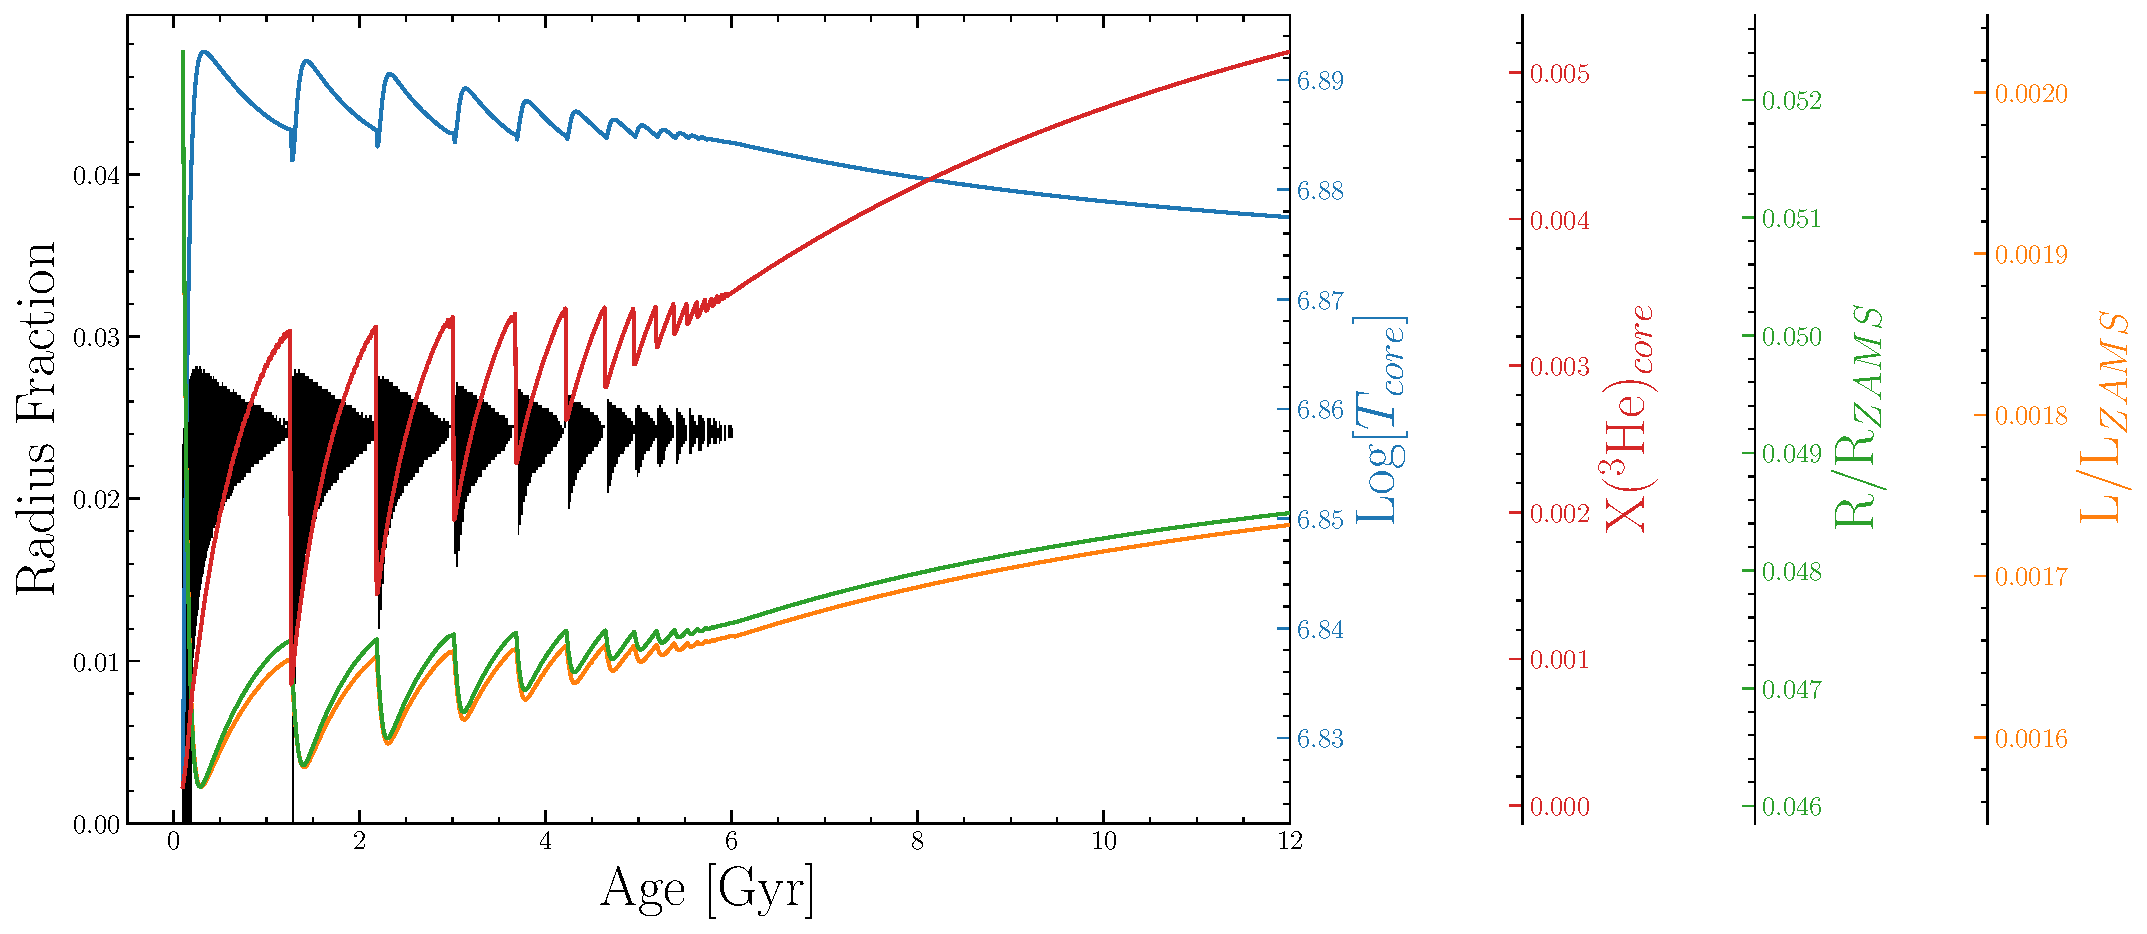
\includegraphics[width=0.9\textwidth]{figures/jaoMagActivity/Kippenhan_clamped.pdf}
  \caption{Kippenhan-Iben diagram for a 0.345 solar mass star. Note the
  periodic mixing events (where the plotted curves peak).}
  \label{fig:kippenhan}
\end{figure*}

Each synthetic star is assigned some base magnetic activity ($B_{0} \sim
\mathcal{N}(1, \sigma_{B})$) and then the number of mixing events before some age $t$
are counted based on local maxima in the core temperature. The toy magnetic
activity at age $t$ for the model is given in Equation \ref{eqn:activity}. An
example of the magnetic evolution resulting from this model is given in Figure
\ref{fig:simpleB}. Fundamentally, this model presents magnetic
activity variation due to mixing events as a random walk and therefore results will
increasing divergence over time.

\begin{align}\label{eqn:activity}
  B(t) = B_{0} + \sum_{i}B_{i} \sim \mathcal{N}(1, \sigma_{B}) 
\end{align}

\begin{figure}
  \centering
  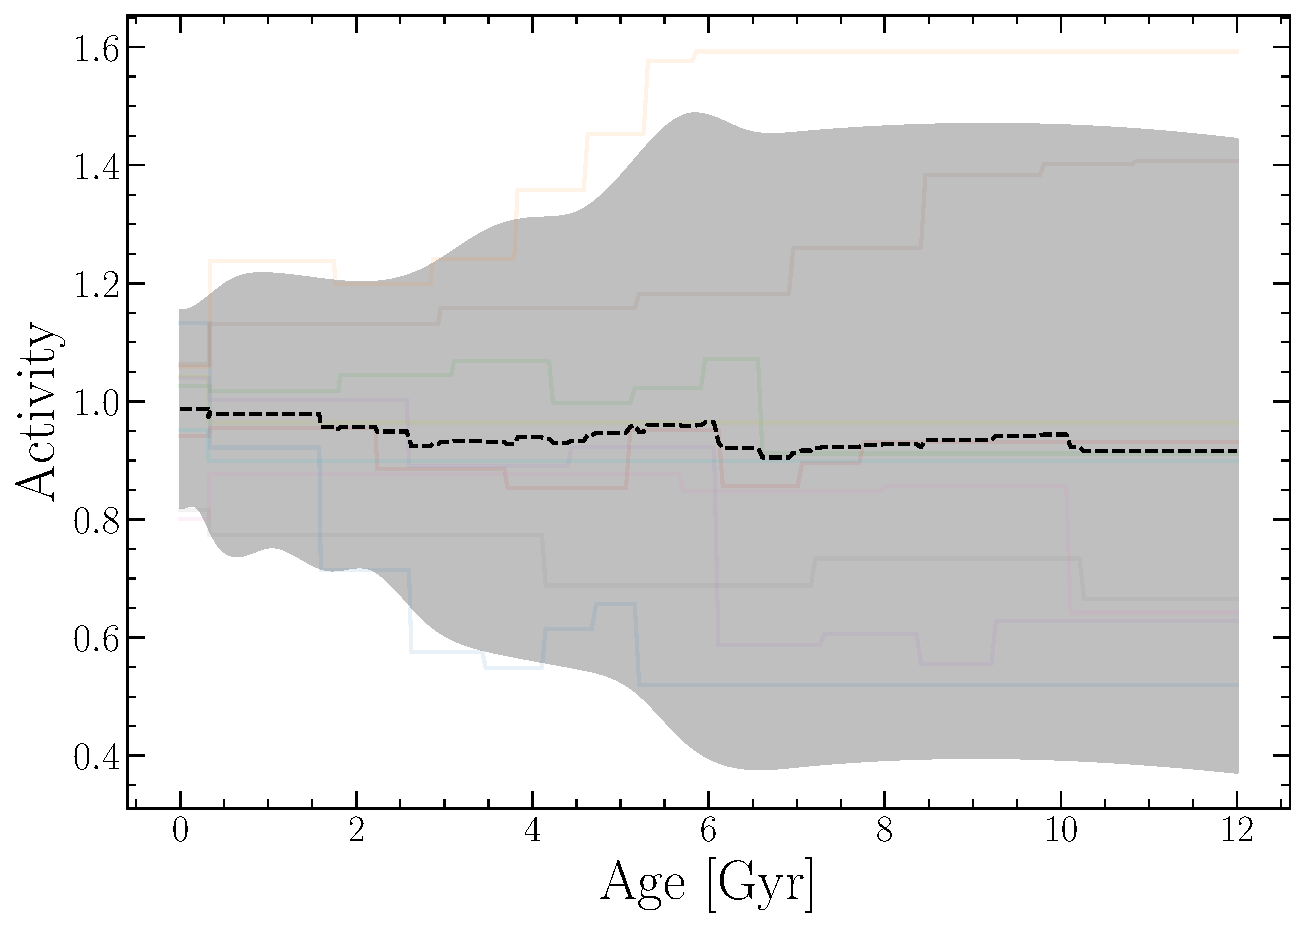
\includegraphics[width=0.85\textwidth]{figures/jaoMagActivity/simpleBEvolution.pdf}
  \caption{Example of the toy model presented here resulting in increased
  divergence between stars magnetic fields. The shaded region represents the
  maximum spread in the two point correlation function at each age.}
  \label{fig:simpleB}
\end{figure}

Applying the same analysis to these models as was done to the observations as
described in Section \ref{sec:results} we find that this simple model results
in a qualitatively similar trend in the standard deviation vs. Magnitude graph
(Figure \ref{fig:model}). In order to reproduce the approximately 50 percent
change to the spread of the activity metric observed in the combined dataset in
section \ref{sec:results} a distribution with a standard deviation of 0.1 is
required when sampling the change in the magnetic activity metric at each
mixing event. This corresponds to 68 percent of mixing events modifying the
activity strength by 10 percent or less. The interpretation here is important:
what this qualitative similarity demonstrates is that it may be reasonable to
expect kissing instabilities to result in the observed increased star-to-star
variation. Importantly, we are not able to claim that kissing instabilities
\textit{do} lead to these increased variations, only that they reasonably
could. Further modeling, observational, and theoretical efforts will be needed
to more definitively answer this question.

\begin{figure}
  \centering
  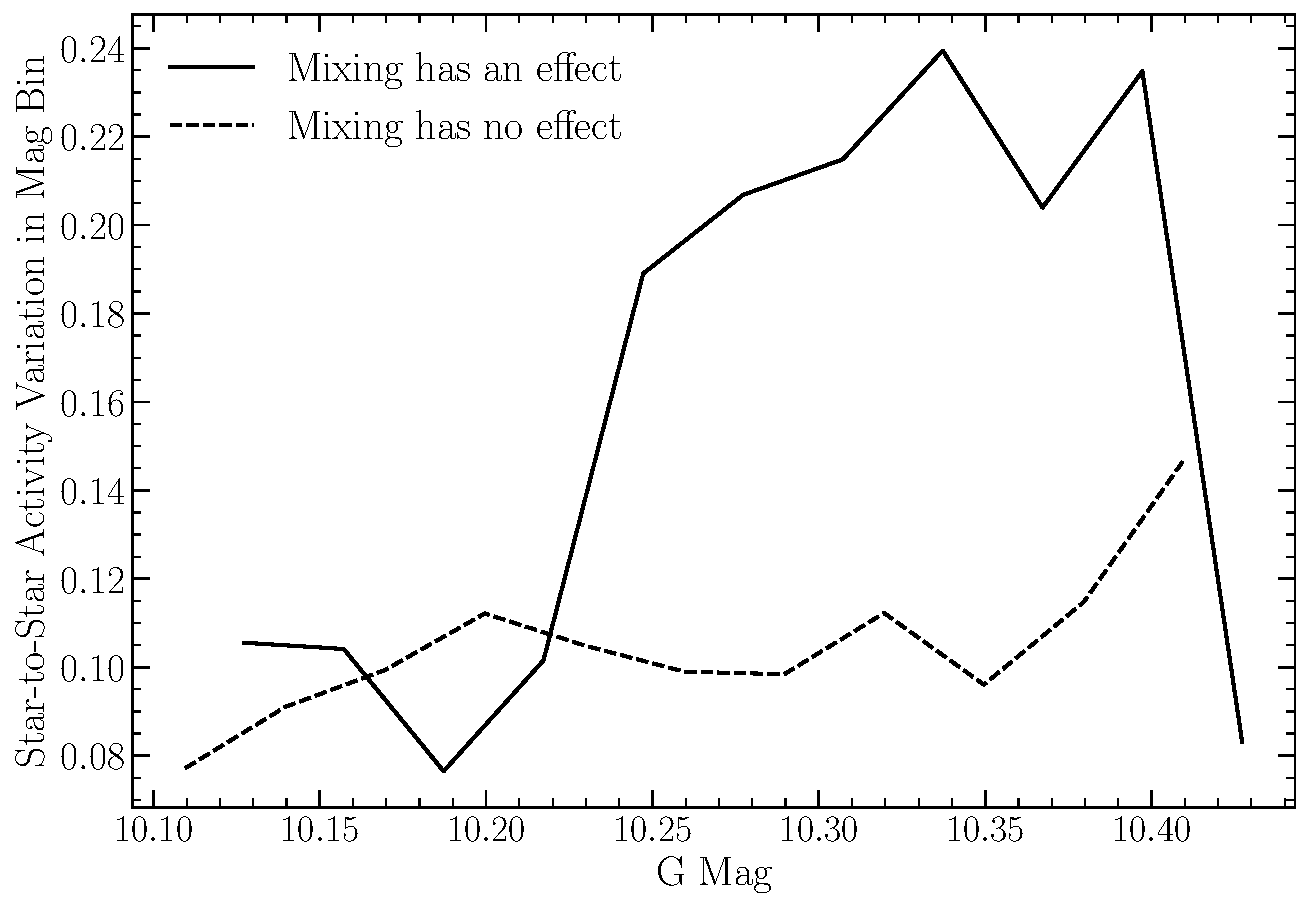
\includegraphics[width=0.85\textwidth]{figures/jaoMagActivity/SpreadModel.pdf}
  \caption{Toy model results showing a qualitatively similar discontinuity in the star-to-star magnetic activity variability.}
  \label{fig:model}
\end{figure}

\subsection{Limitations}
The model presented in this paper is very limited and it is important to keep
these limitations in mind when interpreting the results presented here. Some of
the main challenges which should be leveled at this model are the assumption
that the magnetic field will be altered by some small random perturbation at
every mixing event. This assumption was informed by the large number of free
parameters available to a physical star during the establishment of a large
scale magnetic field and the associated likely stochastic nature of that
process. However, it is similarly believable that the magnetic field will tend
to alter in a uniform manner at each mixing event. For example, since
differential rotation is generally proportional to the temperature gradient
within a star and activity is strongly coupled to differential rotation then it
may be that as the radiative zone reforms over thermal timescales the
homogenization of angular momentum throughout the star results in overall lower
amounts of differential rotation each after mixing event than would otherwise
be present.

Moreover, this model does not consider how other degenerate sources of magnetic
evolution such as stellar spin down, relaxation, or coronal heating may effect
star-to-star variability. These could conceivably lead to a similar increase in
star-to-star variability which is coincident with the Jao Gap magnitude as the
switch from fully to partially convective may effect efficiency of these
process.

Additionally, there are challenges with this toy model that originate from the
stellar evolutionary model. Observations of the Jao Gap show that the feature
is not perpendicular to the magnitude axis; rather, it is inversely
proportional to the color. No models of the Jao Gap published at the time of
writing capture this color dependency and \textit{what causes this color
dependency} remains one of the most pressing questions relating to the
underlying physics. This non captured physics is one potential explanation for
why the magnitude where our model predicts the increase in variability is not
in agreement with where the variability jump exists in the data.

Finally, we have not considered detailed descriptions of the dynamos of stars.
The magneto-hydrodynamical modeling which would be required to model the
evolution of the magnetic field of these stars at thermal timescale resolutions
over gigayears is currently beyond the ability of practical computing.
Therefore future work should focus on limited modeling which may inform the
evolution of the magnetic field directly around the time of a mixing event.

\section{Conclusion}\label{sec:conclusion}
It is, at this point, well established that the Jao Gap may provide a unique view of the interiors of stars for which other probes, such as seismology, fail. However, it has only recently become clear that the Gap may lend insight into not just structural changes within a star but also into the magnetic environment of the star.
\citet{Jao2023} presented evidence that the physics driving the Gap might additionally result in a paucity of H$\alpha$ emission. These authors propose potential physical mechanisms which could explain this paucity, including the core of the star acting as an angular momentum sink during mixing events.

Here we have expanded upon this work by probing the degree and variability of
Calcium II H\&K emission around the Jao Gap. We lack the same statistical
power of \citeauthor{Jao2023}'s sample; however, by focusing on the
star-to-star variability within magnitude bins we are able to retain
statistical power. We find that there is an anomalous increase in variability
at a G magnitude of $\sim 11$. This is only slightly below the observed mean gap magnitude.

Additionally, we propose a simple model to explain this variability. Making the
assumption that the periodic convective mixing events will have some small but
random effect on the overall magnetic field strength we are able to
qualitatively reproduce the increase activity spread in a synthetic population
of stars. 



\part{Individual Stars}
\chapter{Magnetic Fields In M Dwarfs}
\section{Magnetic Activity in M dwarfs} \label{sec:magActivity-intro}
M-dwarfs are the most numerous stars in our galaxy; however, spun-up M-dwarfs
are more magnetically active when compared to larger and hotter stars
\citep{Haw91, Del98, Sch14}. The increase in activity may accelerate the
stripping of an orbiting planet's atmosphere \citep[e.g.][]{Owe16}, and may
dramatically impact habitability \citep{Shi16}. Therefore, it is essential to
understand the magnetic activity of M-dwarfs in order to constrain the
potential habitability and history of the planets that orbit them.
Additionally, rotation and activity may impact the detectability of hosted
planets \citep[e.g.][]{Rob14, Newton2016, Van16}.

Robust theories explaining the origin of solar-like magnetic fields exist and
have proven extensible to other regions of the main sequence \citep{Cha14}. The
classical $\alpha\Omega$ dynamo relies on differential rotation between layers
of a star to stretch a seed poloidal field into a toroidal field \citep{Par55,
Cam17}. Magnetic buoyancy causes the toroidal field to rise through the star.
During this rise, turbulent helical stretching converts the toroidal field back
into a poloidal field \citep{Par55}. Seed fields may originate from the
stochastic movement of charged particles within a star's atmospheres.

In non-fully convective stars the initial conversion of the toroidal field to a
poloidal field is believed to take place at the interface layer between the
radiative and convective regions of a star --- the tachocline \citep{Noy84,
Tom96, Dik99}. The tachocline has two key properties that allow it to play an
important role in solar type magnetic dynamos: 1), there are high shear
stresses, which have been confirmed by astroseismology \citep{Tho96}, and 2),
the density stratification between the radiative and convective zones serves to
``hold'' the newly generated toroidal fields at the tachocline for an extended
time. Over this time, the fields build in strength significantly more than they
would otherwise \citep{Par75}. This theory does not trivially extend to
mid-late M-dwarfs, as they are believed to be fully convective and consequently
do not contain a tachocline \citep{Cha97}. Moreover, fully convective M-dwarfs
are not generally expected to exhibit internal differential rotation
\citep[e.g.][]{barnes2004differential, barnes2005dependence}, though, some
models do produce it \citep{Yad13}.

Currently, there is no single accepted process that serves to build and
maintain fully convective M-dwarf magnetic fields in the same way that the
$\alpha$ and $\Omega$ processes are presently accepted in solar magnetic dynamo
theory. Three-dimensional magneto anelastic hydrodynamical simulations have
demonstrated that local fields generated by convective currents can self
organize into large scale dipolar fields. 
%These fields are similar to smaller scale structure which have been observed through Zeeman-Doppler imaging \citep{Brown2011, Yad15}
These models indicate that for a fully convective star to sustain a magnetic
field it must have a high degree of density stratification --- density
contrasts greater than 20 at the tachocline --- and a sufficiently large magnetic Reynolds
number\footnote{The Reynolds Number is the ratio of magnetic induction to
magnetic diffusion; consequently, a plasma with a larger magnetic Reynolds
number will  sustain a magnetic field for a longer time than a plasma with a
smaller magnetic Reynolds number.}.

An empirical relation between the rotation rate and the level of magnetic
activity has been demonstrated in late-type stars \citep{Skumanich1972, Pal81}. This is
believed to be a result of faster rotating stars exhibiting excess non-thermal
emission from the upper chromosphere or corona when compared to their slower
rotating counterparts. This excess emission is due to magnetic heating of the
upper atmosphere, driven by the underlying stellar dynamo.
The faster a star rotates, up to some saturation threshold, the more such emission is expected. However,
the dynamo process is not dependent solely on rotation; rather, it depends on
whether the contribution from the rotational period ($P_{rot}$) or convective
motion --- parameterized by the convective overturn time scale ($\tau_{c}$) ---
dominates the motion of a charge packet within a star. Therefore, the Rossby
Number ($Ro = P_{rot}/\tau_{c}$) is often used in place of the rotational
period as it accounts for both.

The rotation-activity relation was first discovered using the ratio of X-ray
luminosity to bolometric luminosity ($L_{X}/L_{bol}$) \citep{Pal81} and was
later demonstrated to be a more general phenomenon, observable through other
activity tracers, such as Ca II H\&K emission \citep{Vilhu1984}. This relation has
a number of important structural elements. \citet{Noy84} showed that magnetic
activity as a function of Rossby Number is well modeled as a piecewise power
law relation including a saturated and non-saturated regime. In the saturated
regime, magnetic activity is invariant to changes in Rossby Number; in the
non-saturated regime, activity decreases as Rossby Number increases. The
transition between the saturated and non-saturated regions occurs at $Ro \sim
0.1$ \citep[e.g.][]{Wri11}. Recent evidence may suggest that, instead of an
unsaturated region where activity is fully invariant to rotational period,
activity is more weakly, but still positively, correlated with rotation rate
\citep{Mamajek2008, Reiners2014, Leh20, Magaudda2020}. 

Previous studies of the Ca II H\&K rotation-activity relation
\citep[e.g.][]{Vau81, Sua15, Def17, Hou17} have focused on on spectral ranges
which both extend much earlier than M-dwarfs and which do not fully probe late
M-dwarfs. Other studies have relied on $v\sin(i)$ measurements
\citep[e.g.][]{Browning2010, Hou17}, which are not sensitive to the long
rotation periods reached by slowly rotating, inactive mid-to-late type M dwarfs
\citep[70-150 days:][]{Newton2016}. Therefore, these studies can present only
coarse constraints on the rotation activity relation in the fully convective
regime. The sample we present in this paper is focused on mid-to-late type M
dwarfs, with photometrically measured rotational periods, while maintaining of
order the same number of targets as previous studies.  Consequently, we provide
much finer constraints on the rotation-activity relation in this regime. 

One example of an application of the rotation-activity relation is as a means
of approximating stellar ages. Because as stars spin down, they move along
the rotation-activity relation \citep{Soderblom1991}. To calibrate this
relation, however, one needs a priori knowledge of a star's age and therefore
stars need to be in clusters where population statistics may be used to
accurately measure ages. This has proved doable for FGK type stars; however,
as is often the case, M-dwarfs pose some unique challenges. 

Firstly, the sample of all clusters in which we can observe M-dwarfs is
extremely small due to M-dwarfs' low luminosities. Secondly, open clusters
preferentially contain stars younger than the characteristic time it takes an
M-dwarf to spin down out of the saturated regime of the rotation-activity
relation \citep{West2009, Newton2016, Giacobbe2020}. Therefore, even in the
small set of clusters with measured ages and that contain observable
mid-to-late M-dwarfs, the unsaturated regimes in the rotation-activity
relation is not present. Currently, their has not been a successful
demonstration of using the M-dwarf rotation-activity relation to measure
ages.

We present a high resolution spectroscopic study of 53 mid-late M-dwarfs. We
measure Ca II H\&K strengths, quantified through the $R'_{HK}$ metric, which is
a bolometric flux normalized version of the Mount Wilson S-index. These
activity tracers are then used in concert with photometrically determined
rotational periods, compiled by \citet{Newton2017}, to generate a
rotation--activity relation for our sample. This paper is organized as follows:
Section \ref{sec:Observations} provides an overview of the observations and
data reduction, Section \ref{sec:Analysis} details the analysis of our data,
and Section \ref{sec:results} presents our results and how they fit within the
literature. 

\section{Observations \& Data Reduction}\label{sec:Observations}
We \textbf{initially} selected a sample of 55 mid-late M-dwarfs from targets of
the MEarth survey \citep{Ber12} to observe. Targets were selected based on high
proper motions and availability of a previously measured photometric rotation
period, or an expectation of a measurement based on data available from
MEarth-South at the time. These rotational periods were derived photometrically
\citep[e.g.][]{Newton2016,Man16,Med20}. For star 2MASS J06022261-2019447, which
was categorized as an ``uncertain detection'' from MEarth photometry by
\citet{Newton2018}, including new data from MEarth DR10 we find a period of 95
days. This value was determined following similar methodology to \citet{Irw11}
and \citet{Newton2016,Newton2018}, and is close to the reported candidate
period of 116 days.  References for all periods are provided in the machine
readable version of Table \ref{tab:finalData}.   

High resolution spectra were collected from March to October 2017 using the
Magellan Inamori Kyocera Echelle (MIKE) spectrograh on the 6.5 meter Magellan 2
telescope at the Las Campanas Observatory in Chile. MIKE is a high resolution
double echelle spectrograph with blue and red arms. Respectively, these cover
wavelengths from 3350 - 5000 \AA\ and 4900-9500 \AA\ \citep{Ber03}. We
collected data using a 0.75x5.00" slit resulting in a resolving power of 32700.
Each science target was observed an average of four times with mean integration
times per observation ranging from 53.3 to 1500 seconds. \textbf{Ca II H\&K
lines were observed over a wide range of signa-to-noise ratios, from $\sim 5$ up
to $\sim 240$ with mean and median values of 68 and 61 respectively.}

We use the \texttt{CarPy} pipeline \citep{Kel00, Kel03} to reduce our blue arm
spectra. \texttt{CarPy}'s data products are wavelength calibrated, blaze
corrected, and background subtracted spectra comprising 36 orders. We shift all
resultant target spectra into the rest frame by cross correlating against a
velocity template spectrum. For the velocity template we use an observation of
Proxima Centari in our sample. This spectrum's velocity is both barycentrically
corrected, using astropy's \texttt{SkyCoord} module \citep{Ast18}, and
corrected for Proxima Centari's measured radial velocity, -22.4 km s$^{-1}$
\citep{Tor06}. Each echelle order of every other target observation is cross
correlated against the corresponding order in the template spectra using
\texttt{specutils} \texttt{template\_correlate} function \citep{Nic21}.
Velocity offsets for each order are inferred from a Gaussian fit to the
correlation vs. velocity lag function. For each target, we apply a three sigma
clip to list of echelle order velocities, visually verifying this clip removed
low S/N orders. We take the mean of the sigma-clipped velocities Finally, each
wavelength bin is shifted according to its measured velocity.

Ultimately, two targets (2MASS J16570570-0420559 and 2MASS J04102815-5336078)
had S/N ratios around the Ca II H\&K lines which were too low to be of use,
reducing the number of R'$_{HK}$ measurement we can make from 55 to 53. 

\section{Analysis}\label{sec:Analysis}
Since the early 1960s, the Calcium Fraunhaufer lines have been used as
chromospheric activity tracers \citep{Wil63}. Ca II H\&K lines are observed as
a combination of a broad absorption feature originating in the upper
photosphere along with a narrow emission feature from non-thermal heating of
the upper chromosphere \citep{Catalano1983}. Specifically, the ratio between
emission in the Ca II H\&K lines and flux contributed from the photosphere is
used to define an activity metric known as the S-index \citep{Wil68}.   The
S-index increases with increasing magnetic activity. The S-index is defined as 

\begin{equation}\label{eqn:SIndex}
    S = \alpha \frac{f_{H} + f_{K}}{f_{V} + f_{R}}    
\end{equation}

\noindent where $f_{H}$  and $f_{K}$ are the integrated flux over triangular
passbands with a full width at half maximum of $1.09\text{ \AA}$ centered at
$3968.47\text{ \AA}$ and $3933.66\text{ \AA}$, respectively. The values of
$f_{V}$ and $f_{R}$ are integrated, top hat, broadband regions. They
approximate the continuum (Figure \ref{fig:SindexBandpass}) and are centered at
3901 \AA \ and 4001 \AA \ respectively, with widths of 20 \AA \ each. Finally,
$\alpha$ is a scaling factor with $\alpha = 2.4$.

\begin{figure*}[ht!]
    \centering
    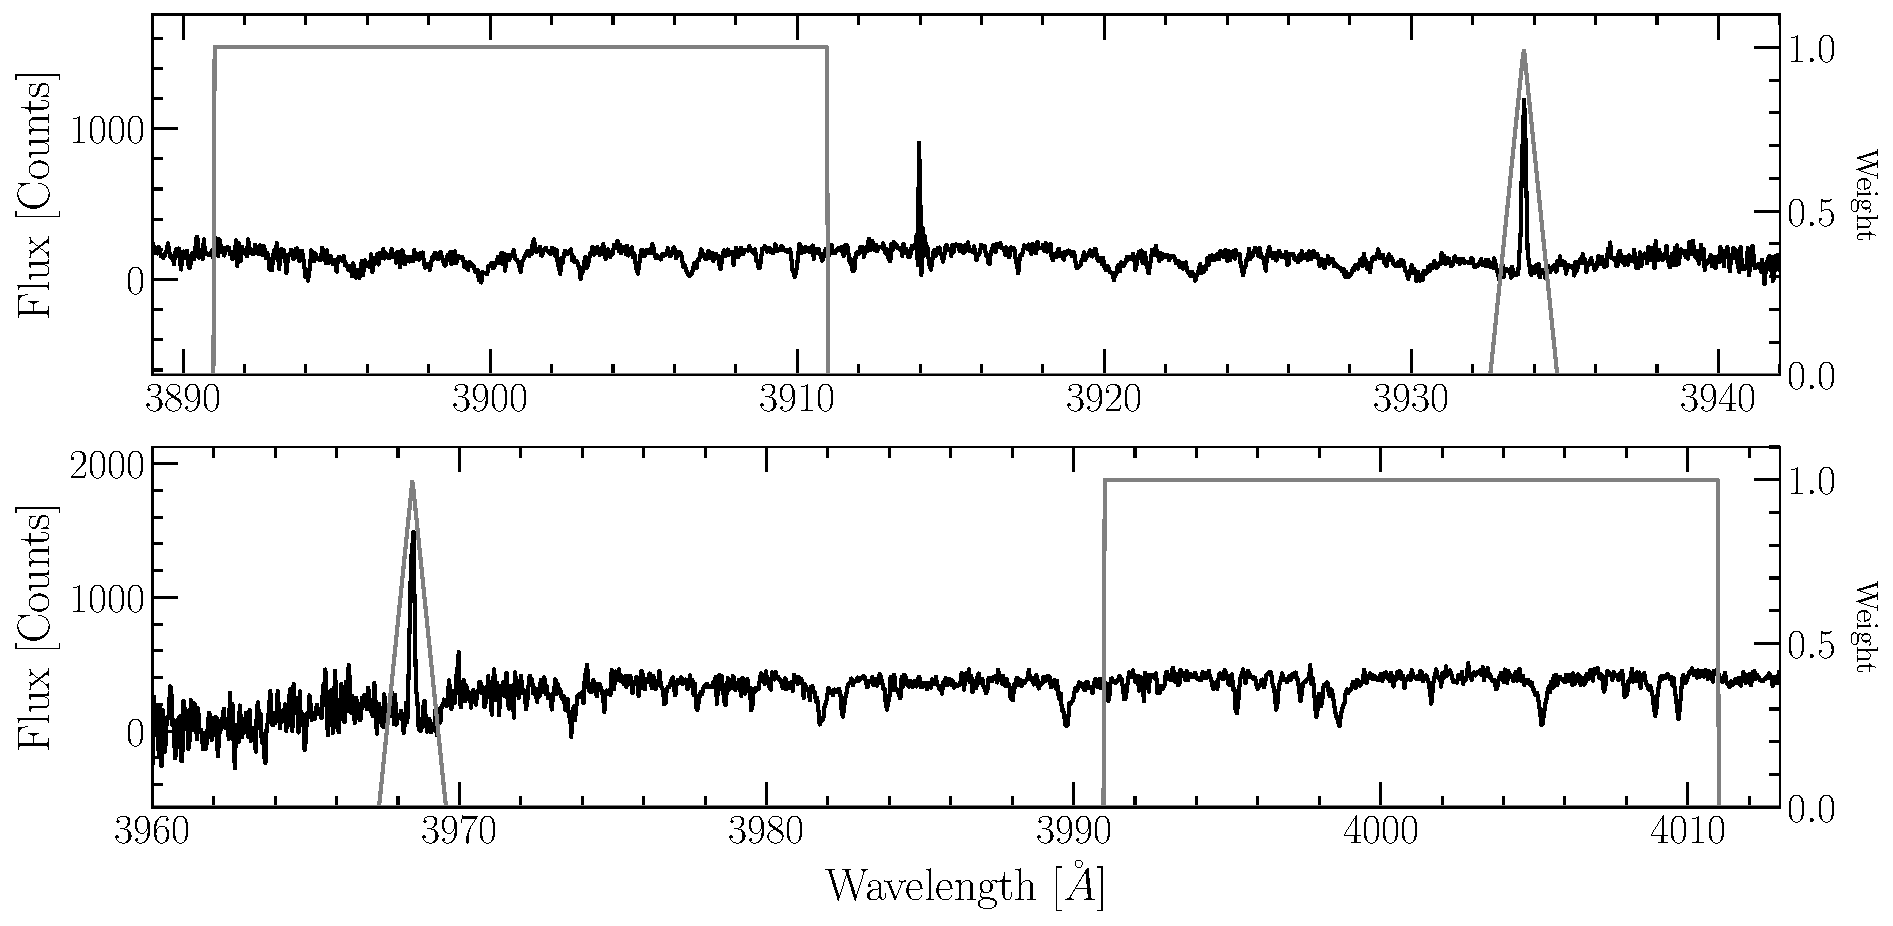
\includegraphics[width=0.9\textwidth]{figures/magActivity/SIndexBandpass.pdf}
	\caption{Spectrum of 2MASS J06105288-4324178 overplotted with the S index
	bandpasses. (top) V band and Ca II K emission line. (bottom) Ca II H
	emission line and R band. Note that the rectangular and triangular
	regions denote both the wavelength range of the band and the relative
	weight assigned to each wavelength in the band while integrating. }
    \label{fig:SindexBandpass}
\end{figure*}

Following the procedure outlined in \citet{Lov11} we use the mean flux per
wavelength interval, $\tilde{f_{i}}$, as opposed to the integrated flux over
each passband when computing the S-index. This means that for each passband,
$i$, with a blue most wavelength $\lambda_{b,i}$ and a red most wavelength
$\lambda_{r,i}$, $\tilde{f}_{i}$ is the summation of the product of flux ($f$)
and weight ($w_{i})$ over the passband.

\begin{equation}\label{eqn:meanFlux}
    \tilde{f}_{i} = \frac{\sum_{l = \lambda_{b,i}}^{\lambda_{r,i}}f(l)w_{i}(l)}{\lambda_{r,i}-\lambda_{b,i}}    
\end{equation}
\noindent where $w_{i}$ represents the triangular passband for $f_{H}$ \& $f_{K}$ and the tophat for $f_{V}$ \& $f_{R}$.

Additionally, the spectrograph used at Mount Wilson during the development of
the S-index exposed the H \& K lines for eight times longer than the continuum
of the spectra. Therefore, for a modern instrument that exposes the entire
sensor simultaneously, there will be 8 times less flux in the Ca II H\&K
passbands than the continuum passbands than for historical observations. This
additional flux is accounted for by defining a new constant $\alpha_{H}$,
defined as:

\begin{equation}
    \alpha_{H} = 8\alpha\left(\frac{1.09\text{ \AA}}{20\text{ \AA}}\right)
\end{equation}
Therefore, S-indices are calculated here not based on the historical definition
given in Equation \ref{eqn:SIndex}; rather, the slightly modified version:

\begin{equation}\label{eqn:finalSIndex}
    S = \alpha_{H}\frac{\tilde{f}_{H} + \tilde{f}_{K}}{\tilde{f}_{V} + \tilde{f}_{R}}
\end{equation}

The S-index may be used to make meaningful comparisons between stars of similar
spectral class; however, it does not account for variations in photospheric
flux and is therefore inadequate for making comparisons between stars of
different spectral classes. The $R'_{HK}$ index \citep{Middelkoop1982} is a
transformation of the S-index intended to remove the contribution of the
photosphere. 

$R'_{HK}$ introduces a bolometric correction factor, $C_{cf}$, developed by
\citet{Middelkoop1982} and later improved upon by \citet{Rutten1984}.
Calibrations of $C_{cf}$ have focused on FGK-type stars using broad band color
indices, predominately B-V. However, these FGK-type solutions do not extend to
later type stars easily as many mid-late M-dwarfs lack B-V photometry.
Consequently, $C_{cf}$ based on B-V colors were never calibrated for M-dwarfs
as many M-dwarfs lack B and V photometry. \citet{SuarezMascareno2016} provided
the first $C_{cf}$ calibrations for M-dwarfs using the more appropriate color
index of $V-K$. The calibration was later extended by \citet{Def17}, which we
adopt here. 

Generally $R'_{HK}$ is defined as

\begin{equation}\label{eqn:RpHKDef}
    R'_{HK} = K\sigma^{-1}10^{-14}C_{cf}(S-S_{phot})
\end{equation}
where K is a factor to scale surface fluxes of arbitrary units into physical
units; the current best value for K is taken from \citet{Hal07},
$K=1.07\times10^{6}\text{erg cm$^{-2}$ s$^{-1}$}$. $S_{phot}$ is the
photospheric contribution to the S-index; in the spectra this manifests as the
broad absorption feature wherein the narrow Ca II H\&K emission resides.
$\sigma$ is the Stephan-Boltzmann constant. If we define 

\begin{equation}
    R_{phot}\equiv K\sigma^{-1}10^{-14}C_{cf}S_{phot}
\end{equation}
then we may write $R'_{HK}$ as 

\begin{equation}\label{eqn:RpHKFinal}
    R'_{HK} = K\sigma^{-1}10^{-14}C_{cf}S - R_{phot}.
\end{equation}

We use the color calibrated coefficients for $\log_{10}(C_{cf})$ and
$\log_{10}(R_{phot})$ presented in Table 1 of \citet{Def17}.

We estimate the uncertainty of $R'_{HK}$ as the standard deviation of a
distribution of $R'_{HK}$ measurements from 5000 Monte Carlo tests. For each
science target we offset the flux value at each wavelength bin by an amount
sampled from a normal distribution. The standard deviation of this normal
distribution is equal to the estimated error at each wavelength bin. These
errors are calculated at reduction time by the pipeline. The R$'_{HK}$
uncertainty varies drastically with signal-to-noise; targets with
signal-to-noise ratios $\sim 5$ have typical uncertainties of a few percent
whereas targets with signal-to-noise ratios $\sim 100$ have typical
uncertainties of a few tenth of a percent.

\subsection{Rotation and Rossby Number}
The goal of this work is to constrain the rotation activity relation;
therefore, in addition to the measured $R'_{HK}$ value, we also need the
rotation of the star. As mentioned, one of the selection criteria for targets
was that their rotation periods were already measured; however, ultimately
6 of the 53 targets with acceptable S/N did not have well constrained
rotational periods. We therefore only use the remaining 47 targets to fit the
rotation-activity relation. 

In order to make the most meaningful comparison possible we transform rotation
period into Rossby Number . This transformation was done using the convective
overturn timescale, $\tau_{c}$, such that the Rossby Number, $Ro =
P_{rot}/\tau_{c}$ . To first order $\tau_{c}$ can be approximated as $70$ days
for fully-convective M-dwarfs \citep{Pizzolato2000}. However, \citet{Wri18}
Equation (5) presents an empirically calibrated expression for $\tau_{c}$. This
calibration is derived by fitting the convective overturn timescale as a
function of color index, in order to minimize the horizontal offset between
stars of different mass in the rotation-activity relationship.  The calibration
from \citet{Wri18} that we use to find convective overturn timescales and
subsequently Rossby numbers is:

\begin{equation}\label{eqn:convectiveOverturn}
    \log_{10}(\tau_{c}) = (0.64\pm0.12)+(0.25\pm0.08)(V-K)
\end{equation}
We adopt symmetric errors for the parameters of Equation
\ref{eqn:convectiveOverturn} equal to the larger of the two anti-symmetric
errors presented in \citet{Wri18} Equation 5. 

\section{Rotation--Activity Relation}\label{sec:results}
We show our rotation-activity relation in Figures
\ref{fig:RpHKvsRossbySelf} \& \ref{fig:RpHKvsRossbyDef}. Note that
errors are shown in both figures; however, they render smaller than the data
point size. Ca II H\&K is also known to be time variable
\citep[e.g.][]{Baroch2020,Perdelwitz2021}, which is not captured in our
single-epoch data. There is one target cut off by the domain of this graph,
2MASS J10252645+0512391. This target has a measured vsini of $59.5\pm2.1$ km
s$^{-1}$ \citep{Kesseli2018} and is therefore quite rotationally broadened, which
is known to affect $R'_{HK}$ measurements \citep[figure 8]{Schroder2009}. The
data used to generate this figure is given in Table \ref{tab:finalData}. Table
\ref{tab:finalData} includes uncertainties, the R'$_{HK}$ measurements for
stars which did not have photometrically derived rotational periods in MEarth,
and data for 2MASS J10252645+0512391

We find a rotation activity relationship qualitatively similar to that
presented in \citet{Def17}. Our rotation activity relationship exhibits both
the expected saturated and unsaturated regimes --- the flat region at $Ro <
Ro_{s}$ and the sloped region at $Ro \geq Ro_{s}$ respectively. We fit the
rotation activity relation given in Equation \ref{eqn:fitEqn} to our data using
Markov Chain Monte Carlo (MCMC), implemented in \texttt{pymc}
\citep{Salvatier2016}. 

  \begin{equation}\label{eqn:fitEqn}
      \log(R'_{HK}) = \begin{cases}
          \log(R_{s}) & Ro < Ro_{s} \\
          k\log(Ro) + \log(R_{s}) - k\log(Ro_{s}) & Ro \geq Ro_{s}
      \end{cases}
  \end{equation}

\noindent $Ro_{s}$ is the Rossby number cutoff between the saturated and
unsaturated regime. $R_{s}$ is the maximum, saturated, value of $R'_{HK}$ and
$k$ is the index of the power law when $Ro \geq Ro_{s}$. Due to the
issues measuring $R'_{HK}$ for high vsini targets discussed above, we exclude
2MASS J10252645+0512391 from this fit. All logarithms are base ten unless
another base is explicitly given.
\begin{table}[ht]
  \small
    \centering
    \setlength{\tabcolsep}{4pt}
    \begin{tabular}{lcccccccc}
\hline
2MASS ID & Mass & $Ro$ & $\log(R'_{HK})$ & $\log(R'_{HK})_{err}$ & $V_{mag}$ & $V-K$ & prot & $r_{prot}$\\
 & $\mathrm{M_{\odot}}$ &  &  &  & $\mathrm{mag}$ & $\mathrm{mag}$ & $\mathrm{d}$ &   \\
\hline
\hline
06000351+0242236 & 0.24 & 0.020 & -4.5475 & 0.0021 & 11.31 & 5.268 & 1.809 & 2016ApJ...821...93N  \\
02125458+0000167 & 0.27 & 0.048 & -4.6345 & 0.0014 & 13.58 & 5.412 & 4.732 & 2016ApJ...821...93N  \\
01124752+0154395 & 0.28 & 0.026 & -4.4729 & 0.0017 & 14.009 & 5.240 & 2.346 & 2016ApJ...821...93N  \\
10252645+0512391 & 0.11 & 0.000 & -4.9707 & 0.0380 & 18.11 & 7.322 & 0.102 & 2016ApJ...821...93N  \\
05015746-0656459 & 0.17 & 0.873 & -5.0049 & 0.0028 & 12.2 & 5.464 & 88.500 & 2012AcA....62...67K  \\
06022261-2019447 & 0.23 & 1.307 & -5.6980 & 0.0192 & 13.26 & 4.886 & 95.000 & This Work  \\
06105288-4324178 & 0.30 & 0.705 & -5.2507 & 0.0139 & 12.28 & 4.968 & 53.736 & 2018AJ....156..217N  \\
09442373-7358382 & 0.24 & 0.542 & -5.6026 & 0.0147 & 15.17 & 5.795 & 66.447 & 2018AJ....156..217N  \\
14211512-0107199 & 0.24 & 1.160 & -5.5846 & 0.0125 & 13.12 & 5.027 & 91.426 & 2018AJ....156..217N  \\
14294291-6240465 & 0.12 & 0.394 & -5.0053 & 0.0014 & 11.13 & 6.746 & 83.500 & 1998AJ....116..429B  \\
16352464-2718533 & 0.23 & 1.423 & -5.5959 & 0.0108 & 14.18 & 5.182 & 122.656 & 2018AJ....156..217N  \\
16570570-0420559 & 0.24 & 0.014 & -4.3071 & 0.0014 & 12.25 & 5.130 & 1.212 & 2012AcA....62...67K  \\
02004725-1021209 & 0.34 & 0.188 & -4.7907 & 0.0026 & 14.118 & 5.026 & 14.793 & 2018AJ....156..217N  \\
18494929-2350101 & 0.18 & 0.034 & -4.5243 & 0.0015 & 10.5 & 5.130 & 2.869 & 2007AcA....57..149K  \\
20035892-0807472 & 0.33 & 0.946 & -5.6530 & 0.0077 & 13.54 & 5.254 & 84.991 & 2018AJ....156..217N  \\
21390081-2409280 & 0.21 & 1.152 & -6.1949 & 0.0190 & 13.45 & 5.091 & 94.254 & 2018AJ....156..217N  \\
23071524-2307533 & 0.30 & 0.720 & -5.2780 & 0.0077 & 13.587 & 4.849 & 51.204 & 2018AJ....156..217N  \\
00094508-4201396 & 0.30 & 0.009 & -4.3392 & 0.0018 & 13.62 & 5.397 & 0.859 & 2018AJ....156..217N  \\
00310412-7201061 & 0.31 & 0.906 & -5.3879 & 0.0074 & 13.69 & 5.245 & 80.969 & 2018AJ....156..217N  \\
01040695-6522272 & 0.17 & 0.006 & -4.4889 & 0.0024 & 13.98 & 5.448 & 0.624 & 2018AJ....156..217N  \\
02014384-1017295 & 0.19 & 0.034 & -4.5400 & 0.0022 & 14.473 & 5.284 & 3.152 & 2018AJ....156..217N  \\
03100305-2341308 & 0.40 & 0.028 & -4.2336 & 0.0017 & 13.502 & 4.935 & 2.083 & 2018AJ....156..217N  \\
03205178-6351524 & 0.33 & 1.029 & -5.6288 & 0.0096 & 13.433 & 5.238 & 91.622 & 2018AJ....156..217N  \\
07401183-4257406 & 0.15 & 0.002 & -4.3365 & 0.0022 & 13.81 & 6.042 & 0.307 & 2018AJ....156..217N  \\
08184619-4806172 & 0.37 & 0.021 & -4.2834 & 0.0025 & 14.37 & 5.019 & 1.653 & 2018AJ....156..217N  \\
08443891-4805218 & 0.20 & 1.348 & -5.6682 & 0.0067 & 13.932 & 5.370 & 129.513 & 2018AJ....156..217N  \\
09342791-2643267 & 0.19 & 0.007 & -4.3415 & 0.0025 & 13.992 & 5.373 & 0.694 & 2018AJ....156..217N  \\
09524176-1536137 & 0.26 & 1.342 & -5.6319 & 0.0110 & 13.43 & 4.923 & 99.662 & 2018AJ....156..217N  \\
11075025-3421003 & 0.25 & 0.068 & -4.2250 & 0.0032 & 15.04 & 5.633 & 7.611 & 2018AJ....156..217N  \\
11575352-2349007 & 0.39 & 0.031 & -4.2952 & 0.0026 & 14.77 & 5.415 & 3.067 & 2018AJ....156..217N  \\
12102834-1310234 & 0.36 & 0.435 & -4.6892 & 0.0029 & 13.83 & 5.418 & 42.985 & 2018AJ....156..217N  \\
12440075-1110302 & 0.18 & 0.020 & -4.4053 & 0.0033 & 14.22 & 5.546 & 2.099 & 2018AJ....156..217N  \\
13442092-2618350 & 0.35 & 2.032 & -5.9634 & 0.0253 & 13.253 & 4.968 & 154.885 & 2018AJ....156..217N  \\
14253413-1148515 & 0.51 & 0.301 & -4.7641 & 0.0030 & 13.512 & 5.121 & 25.012 & 2018AJ....156..217N  \\
14340491-1824106 & 0.38 & 0.271 & -4.6093 & 0.0038 & 14.346 & 5.638 & 30.396 & 2018AJ....156..217N  \\
15154371-0725208 & 0.38 & 0.050 & -4.6214 & 0.0023 & 12.93 & 5.224 & 4.379 & 2018AJ....156..217N  \\
15290145-0612461 & 0.46 & 0.095 & -4.2015 & 0.0017 & 14.011 & 5.230 & 8.434 & 2018AJ....156..217N  \\
16204186-2005139 & 0.45 & 0.031 & -4.3900 & 0.0035 & 13.68 & 5.261 & 2.814 & 2018AJ....156..217N  \\
16475517-6509116 & 0.17 & 0.889 & -4.8744 & 0.0045 & 13.98 & 5.101 & 73.142 & 2018AJ....156..217N  \\
20091824-0113377 & 0.15 & 0.010 & -4.3772 & 0.0023 & 14.47 & 5.958 & 1.374 & 2018AJ....156..217N  \\
20273733-5452592 & 0.35 & 1.520 & -5.9982 & 0.0181 & 13.18 & 5.259 & 136.924 & 2018AJ....156..217N  \\
20444800-1453208 & 0.49 & 0.073 & -4.4912 & 0.0023 & 14.445 & 5.305 & 6.715 & 2018AJ....156..217N  \\
15404341-5101357 & 0.10 & 0.318 & -5.0062 & 0.0081 & 15.26 & 7.317 & 93.702 & 2018AJ....156..217N  \\
22480446-2422075 & 0.20 & 0.005 & -4.4123 & 0.0016 & 12.59 & 5.384 & 0.466 & 2013AJ....146..154M  \\
06393742-2101333 & 0.26 & 0.952 & -5.2524 & 0.0069 & 12.77 & 5.120 & 79.152 & 2018AJ....156..217N  \\
04130560+1514520 & 0.30 & 0.019 & -4.4775 & 0.0088 & 15.881 & 5.437 & 1.881 & 2016ApJ...818..46M  \\
02411510-0432177 & 0.20 & 0.004 & -4.4272 & 0.0016 & 13.79 & 5.544 & 0.400 & 2020ApJ...905..107M  \\
  11381671-7721484 & 0.12 & 0.958 & \textbf{-5.5015} & 0.0369 & 14.78 & 6.259 & 153.506 & This Work  \\
  12384914-3822527 & 0.15 & 2.527 & \textbf{-6.0690} & 0.0156 & 12.75 & 5.364 & 241.913 & This Work  \\
  13464102-5830117 & 0.48 & 1.340 & \textbf{-5.6977} & 0.0146 &  &  & 65.017 & This Work  \\
  15165576-0037116 & 0.31 & 0.157 & \textbf{-4.0704} & 0.0024 & 14.469 & 5.364 & 15.028 & This Work  \\
  19204795-4533283 & 0.18 & 1.706 & \textbf{-5.8392} & 0.0091 & 12.25 & 5.405 & 167.225 & This Work  \\
  21362532-4401005 & 0.20 & 1.886 & \textbf{-5.8978} & 0.0168 & 14.14 & 5.610 & 207.983 & This Work  \\
\hline
\end{tabular}


% \begin{tabular}{lcccccc}
% \hline
% 	2MASS ID &  Mass &    $Ro$ &  $\log(R'_{HK})$ & $\log(R'_{HK})_{err}$ & $V_{mag}$ &   $V-K$ \\
% \hline
% \hline
% 06000351+0242236 &  0.237 &  0.020 &     -4.548 &          0.002 &  11.310 &  5.268 \\
% 02125458+0000167 &  0.268 &  0.048 &     -4.635 &          0.001 &  13.580 &  5.412 \\
% 01124752+0154395 &  0.278 &  0.026 &     -4.473 &          0.001 &  14.009 &  5.240 \\
% 10252645+0512391 &  0.111 &  0.000 &     -4.971 &          0.007 &  18.110 &  7.322 \\
% 05015746-0656459 &  0.168 &  0.873 &     -5.005 &          0.003 &  12.200 &  5.464 \\
% 06022261-2019447 &  0.234 &  1.307 &     -5.698 &          0.012 &  13.260 &  4.886 \\
% 06105288-4324178 &  0.295 &  0.705 &     -5.251 &          0.008 &  12.280 &  4.968 \\
% 09442373-7358382 &  0.240 &  0.542 &     -5.603 &          0.006 &  15.170 &  5.795 \\
% 14211512-0107199 &  0.238 &  1.160 &     -5.585 &          0.008 &  13.120 &  5.027 \\
% 14294291-6240465 &  0.119 &  0.394 &     -5.005 &          0.001 &  11.130 &  6.746 \\
% 16352464-2718533 &  0.228 &  1.423 &     -5.596 &          0.006 &  14.180 &  5.182 \\
% 16570570-0420559 &  0.242 &  0.014 &     -4.307 &          0.001 &  12.250 &  5.130 \\
% 02004725-1021209 &  0.343 &  0.188 &     -4.791 &          0.002 &  14.118 &  5.026 \\
% 18494929-2350101 &  0.175 &  0.034 &     -4.524 &          0.001 &  10.500 &  5.130 \\
% 20035892-0807472 &  0.328 &  0.946 &     -5.653 &          0.007 &  13.540 &  5.254 \\
% 21390081-2409280 &  0.209 &  1.152 &     -6.195 &          0.015 &  13.450 &  5.091 \\
% 23071524-2307533 &  0.303 &  0.720 &     -5.278 &          0.006 &  13.587 &  4.849 \\
% 00094508-4201396 &  0.304 &  0.009 &     -4.339 &          0.001 &  13.620 &  5.397 \\
% 00310412-7201061 &  0.311 &  0.906 &     -5.388 &          0.006 &  13.690 &  5.245 \\
% 01040695-6522272 &  0.171 &  0.006 &     -4.489 &          0.002 &  13.980 &  5.448 \\
% 02014384-1017295 &  0.193 &  0.034 &     -4.540 &          0.002 &  14.473 &  5.284 \\
% 03100305-2341308 &  0.395 &  0.028 &     -4.234 &          0.001 &  13.502 &  4.935 \\
% 03205178-6351524 &  0.330 &  1.029 &     -5.629 &          0.007 &  13.433 &  5.238 \\
% 07401183-4257406 &  0.154 &  0.002 &     -4.337 &          0.001 &  13.810 &  6.042 \\
% 08184619-4806172 &  0.370 &  0.021 &     -4.283 &          0.001 &  14.370 &  5.019 \\
% 08443891-4805218 &  0.202 &  1.348 &     -5.668 &          0.004 &  13.932 &  5.370 \\
% 09342791-2643267 &  0.192 &  0.007 &     -4.341 &          0.001 &  13.992 &  5.373 \\
% 09524176-1536137 &  0.264 &  1.342 &     -5.632 &          0.007 &  13.430 &  4.923 \\
% 11075025-3421003 &  0.255 &  0.068 &     -4.225 &          0.001 &  15.040 &  5.633 \\
% 11575352-2349007 &  0.393 &  0.031 &     -4.295 &          0.001 &  14.770 &  5.415 \\
% 12102834-1310234 &  0.355 &  0.435 &     -4.689 &          0.002 &  13.830 &  5.418 \\
% 12440075-1110302 &  0.184 &  0.020 &     -4.405 &          0.002 &  14.220 &  5.546 \\
% 13442092-2618350 &  0.348 &  2.032 &     -5.963 &          0.014 &  13.253 &  4.968 \\
% 14253413-1148515 &  0.505 &  0.301 &     -4.764 &          0.002 &  13.512 &  5.121 \\
% 14340491-1824106 &  0.377 &  0.271 &     -4.609 &          0.002 &  14.346 &  5.638 \\
% 15154371-0725208 &  0.378 &  0.050 &     -4.621 &          0.002 &  12.930 &  5.224 \\
% 15290145-0612461 &  0.455 &  0.095 &     -4.201 &          0.001 &  14.011 &  5.230 \\
% 16204186-2005139 &  0.453 &  0.031 &     -4.390 &          0.002 &  13.680 &  5.261 \\
% 16475517-6509116 &  0.170 &  0.889 &     -4.874 &          0.003 &  13.980 &  5.101 \\
% 20091824-0113377 &  0.147 &  0.010 &     -4.377 &          0.001 &  14.470 &  5.958 \\
% 20273733-5452592 &  0.350 &  1.520 &     -5.998 &          0.012 &  13.180 &  5.259 \\
% 20444800-1453208 &  0.485 &  0.073 &     -4.491 &          0.002 &  14.445 &  5.305 \\
% 15404341-5101357 &  0.098 &  0.318 &     -5.006 &          0.003 &  15.260 &  7.317 \\
% 22480446-2422075 &  0.198 &  0.005 &     -4.412 &          0.001 &  12.590 &  5.384 \\
% 06393742-2101333 &  0.258 &  0.952 &     -5.252 &          0.004 &  12.770 &  5.120 \\
% 04130560+1514520 &  0.298 &  0.019 &     -4.477 &          0.004 &  15.881 &  5.437 \\
% 02411510-0432177 &  0.197 &  0.004 &     -4.427 &          0.001 &  13.790 &  5.544 \\
% \hline
% \end{tabular}

% \begin{tabular}{lccccc}
% \hline
% 2MASS ID &  Mass &    $Ro$ &  $\log(R'_{HK})$ &   $V_{mag}$ &   V-K \\
% \hline
% \hline
% J00094508-4201396 &  0.30 &  0.01 &      -4.33 &  13.62 &  5.40 \\
% J00310412-7201061 &  0.31 &  0.91 &      -5.36 &  13.69 &  5.24 \\
% J01040695-6522272 &  0.17 &  0.01 &      -4.47 &  13.98 &  5.45 \\
% J01124752+0154395 &  0.28 &  0.03 &      -4.45 &  14.01 &  5.24 \\
% J02014384-1017295 &  0.19 &  0.03 &      -4.53 &  14.47 &  5.28 \\
% J02125458+0000167 &  0.27 &  0.05 &      -4.63 &  13.58 &  5.41 \\
% J03100305-2341308 &  0.40 &  0.03 &      -4.21 &  13.50 &  4.94 \\
% J03205178-6351524 &  0.33 &  1.03 &      -5.60 &  13.43 &  5.24 \\
% J05015746-0656459 &  0.17 &  0.87 &      -4.98 &  12.20 &  5.46 \\
% J06000351+0242236 &  0.24 &  0.02 &      -4.53 &  11.31 &  5.27 \\
% J06105288-4324178 &  0.30 &  0.71 &      -5.21 &  12.28 &  4.97 \\
% J06105288-4324178 &  0.30 &  0.71 &      -5.21 &  12.28 &  4.97 \\
% J06393742-2101333 &  0.26 &  0.95 &      -5.21 &  12.77 &  5.12 \\
% J06393742-2101333 &  0.26 &  0.95 &      -5.21 &  12.77 &  5.12 \\
% J07401183-4257406 &  0.15 &  0.00 &      -4.28 &  13.81 &  6.04 \\
% J08184619-4806172 &  0.37 &  0.02 &      -4.22 &  14.37 &  5.02 \\
% J08443891-4805218 &  0.20 &  1.35 &      -5.59 &  13.93 &  5.37 \\
% J09342791-2643267 &  0.19 &  0.01 &      -4.31 &  13.99 &  5.37 \\
% J09524176-1536137 &  0.26 &  1.34 &      -5.48 &  13.43 &  4.92 \\
% J11075025-3421003 &  0.25 &  0.07 &      -4.21 &  15.04 &  5.63 \\
% J11575352-2349007 &  0.39 &  0.03 &      -4.28 &  14.77 &  5.41 \\
% J12102834-1310234 &  0.36 &  0.44 &      -4.60 &  13.83 &  5.42 \\
% J12440075-1110302 &  0.18 &  0.02 &      -4.35 &  14.22 &  5.55 \\
% J13442092-2618350 &  0.35 &  2.03 &      -5.74 &  13.25 &  4.97 \\
% J14211512-0107199 &  0.24 &  1.16 &      -5.43 &  13.12 &  5.03 \\
% J14253413-1148515 &  0.51 &  0.30 &      -4.75 &  13.51 &  5.12 \\
% J14294291-6240465 &  0.12 &  0.39 &      -5.00 &  11.13 &  6.75 \\
% J14340491-1824106 &  0.38 &  0.27 &      -4.56 &  14.35 &  5.64 \\
% J15154371-0725208 &  0.38 &  0.05 &      -4.58 &  12.93 &  5.22 \\
% J15290145-0612461 &  0.46 &  0.10 &      -4.44 &  14.01 &  5.23 \\
% J16204186-2005139 &  0.45 &  0.03 &      -4.32 &  13.68 &  5.26 \\
% J16204186-2005139 &  0.45 &  0.03 &      -4.32 &  13.68 &  5.26 \\
% J16352464-2718533 &  0.23 &  1.42 &      -5.46 &  14.18 &  5.18 \\
% J16360563+0848491 &  0.22 &  0.07 &      -3.93 &  13.81 &  5.30 \\
% J16400599+0042188 &  0.18 &  0.00 &      -4.35 &  13.70 &  5.49 \\
% J16570570-0420559 &  0.24 &  0.01 &      -4.28 &  12.25 &  5.13 \\
% J16570570-0420559 &  0.24 &  0.01 &      -4.28 &  12.25 &  5.13 \\
% J18494929-2350101 &  0.18 &  0.03 &      -4.52 &  10.50 &  5.13 \\
% J20035892-0807472 &  0.33 &  0.95 &      -5.65 &  13.54 &  5.25 \\
% J20091824-0113377 &  0.15 &  0.01 &      -4.37 &  14.47 &  5.96 \\
% J20444800-1453208 &  0.49 &  0.07 &      -4.46 &  14.44 &  5.30 \\
% J21390081-2409280 &  0.21 &  1.15 &      -6.16 &  13.45 &  5.09 \\
% J22480446-2422075 &  0.20 &  0.00 &      -4.39 &  12.59 &  5.38 \\
% J22480446-2422075 &  0.20 &  0.00 &      -4.39 &  12.59 &  5.38 \\
% J23071524-2307533 &  0.30 &  0.72 &      -5.28 &  13.59 &  4.85 \\
% J23071524-2307533 &  0.30 &  0.72 &      -5.28 &  13.59 &  4.85 \\
% J23532520-7056410 &  0.26 &  0.01 &      -4.31 &  13.01 &  5.23 \\
% \hline
% \end{tabular}

  \caption{Calculated Rossby Numbers and $R'_{HK}$ values. All circular data
  points in Figures \ref{fig:RpHKvsRossbySelf} \& \ref{fig:RpHKvsRossbyDef} are
  present in this table. Masses are taken from the MEarth database. A machine
  readable version of this table is available. Rows where the activity metric
  is in bold face were estimates derived from our model fit not empirical
  measurements.}
    \label{tab:finalData}
\end{table}
\begin{figure*}
    \centering
    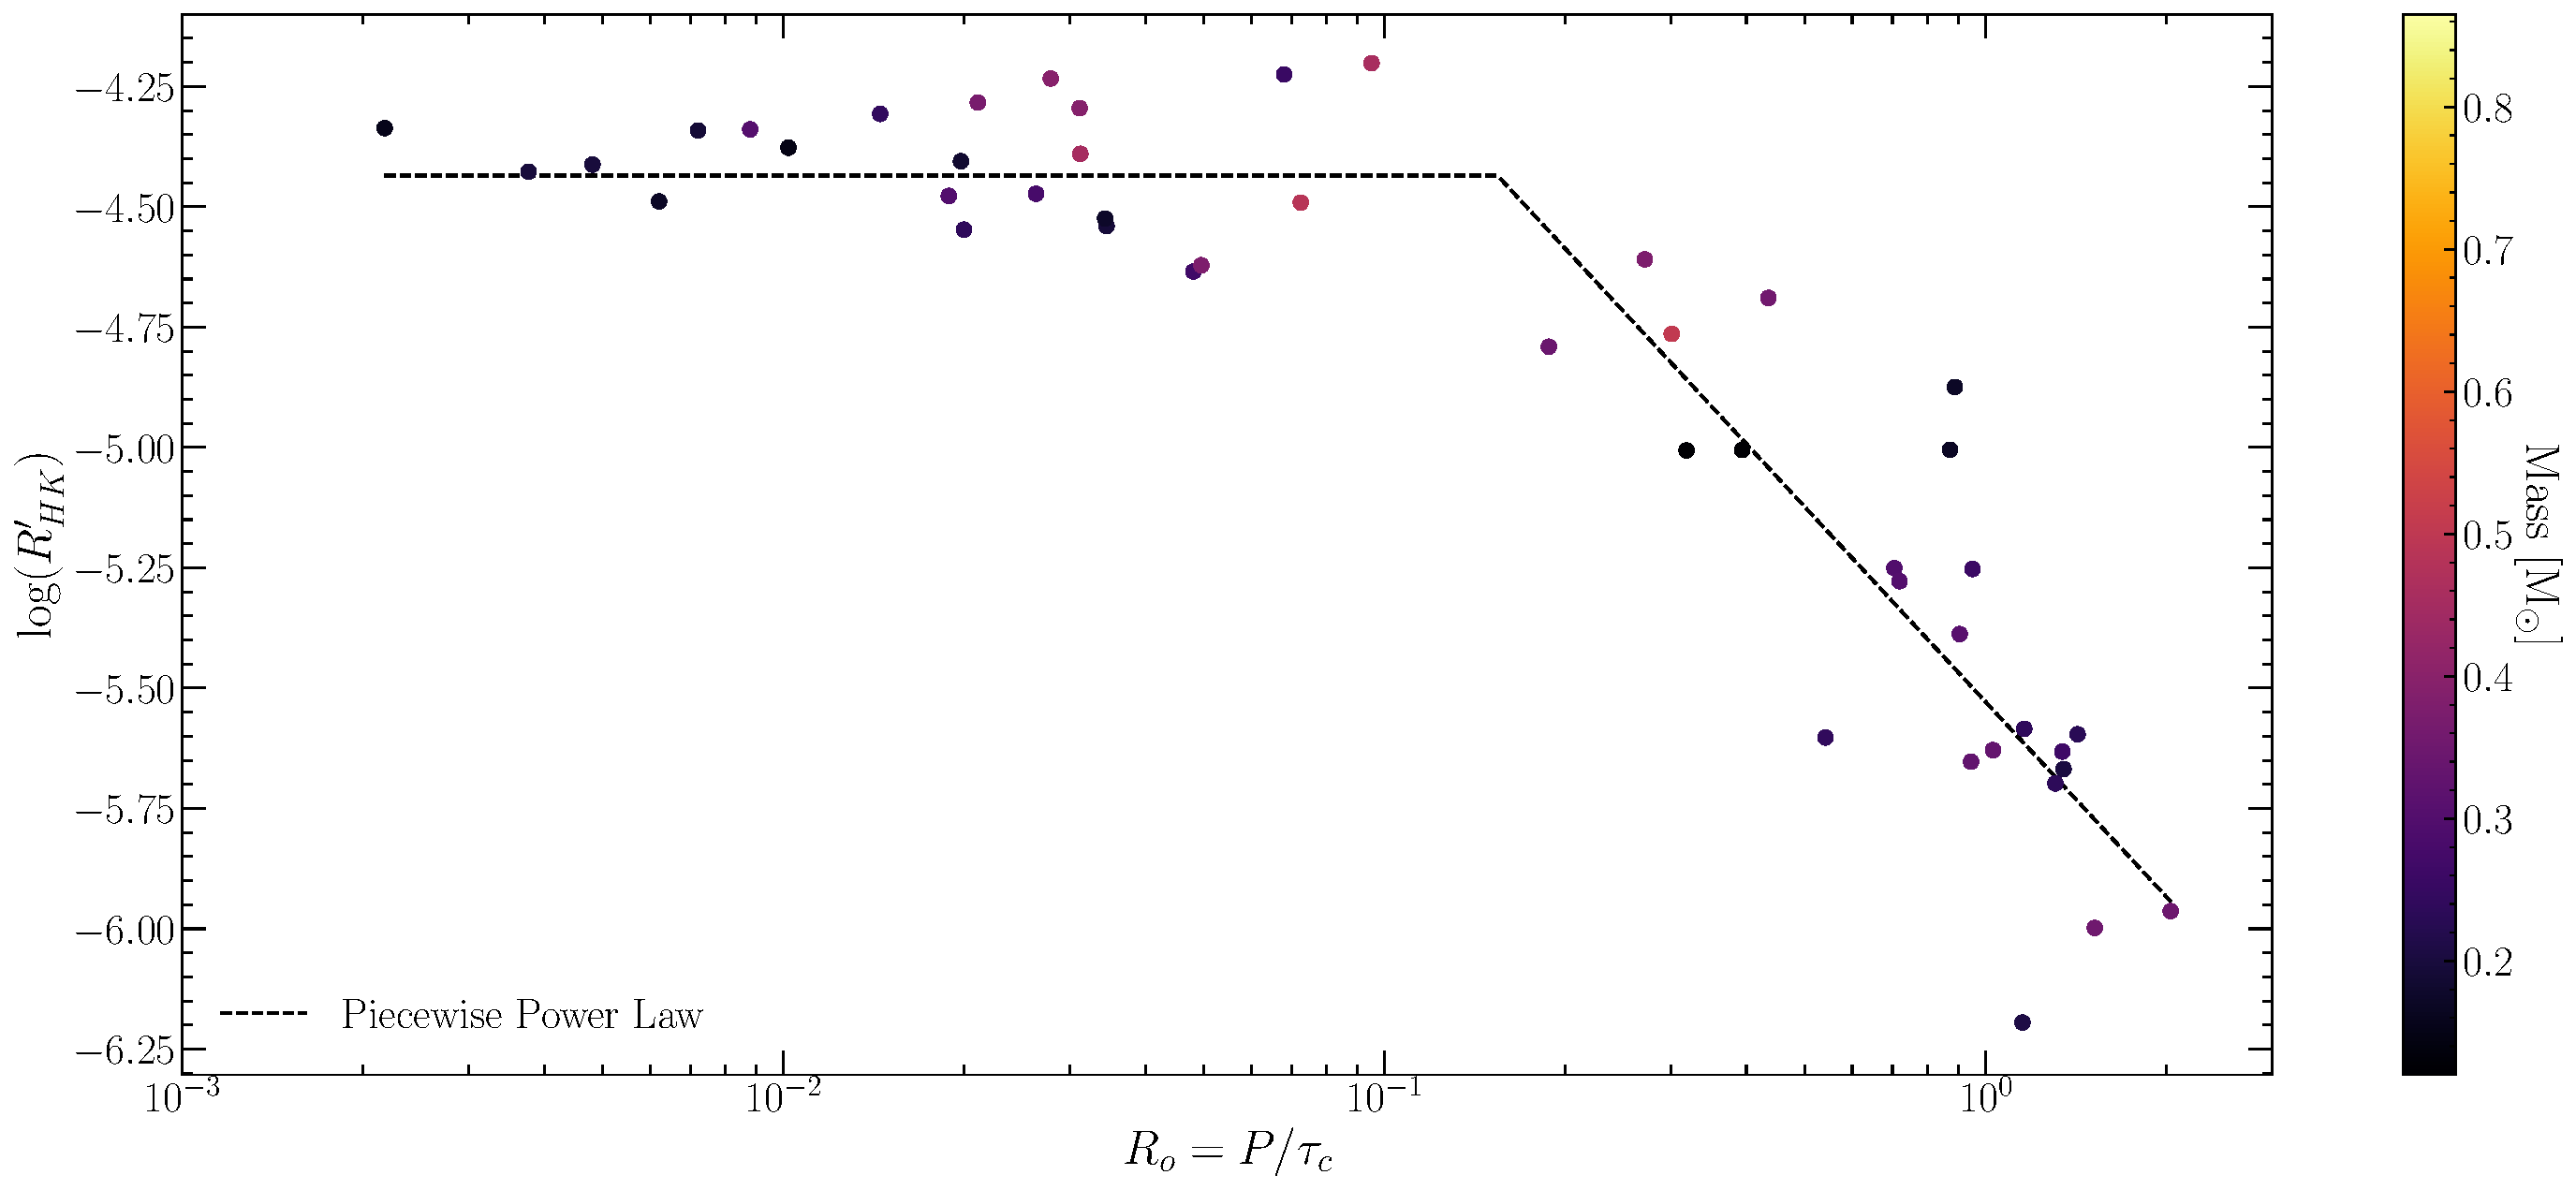
\includegraphics[width=0.9\textwidth]{figures/magActivity/RpHKvsR0_MC_justThisPaper.pdf}
	\caption{Rotation activity relation from this work. The color axis gives
	each stars mass. The dashed line is the best fit to our data set.}
    \label{fig:RpHKvsRossbySelf}
\end{figure*}
\begin{figure*}
    \centering
    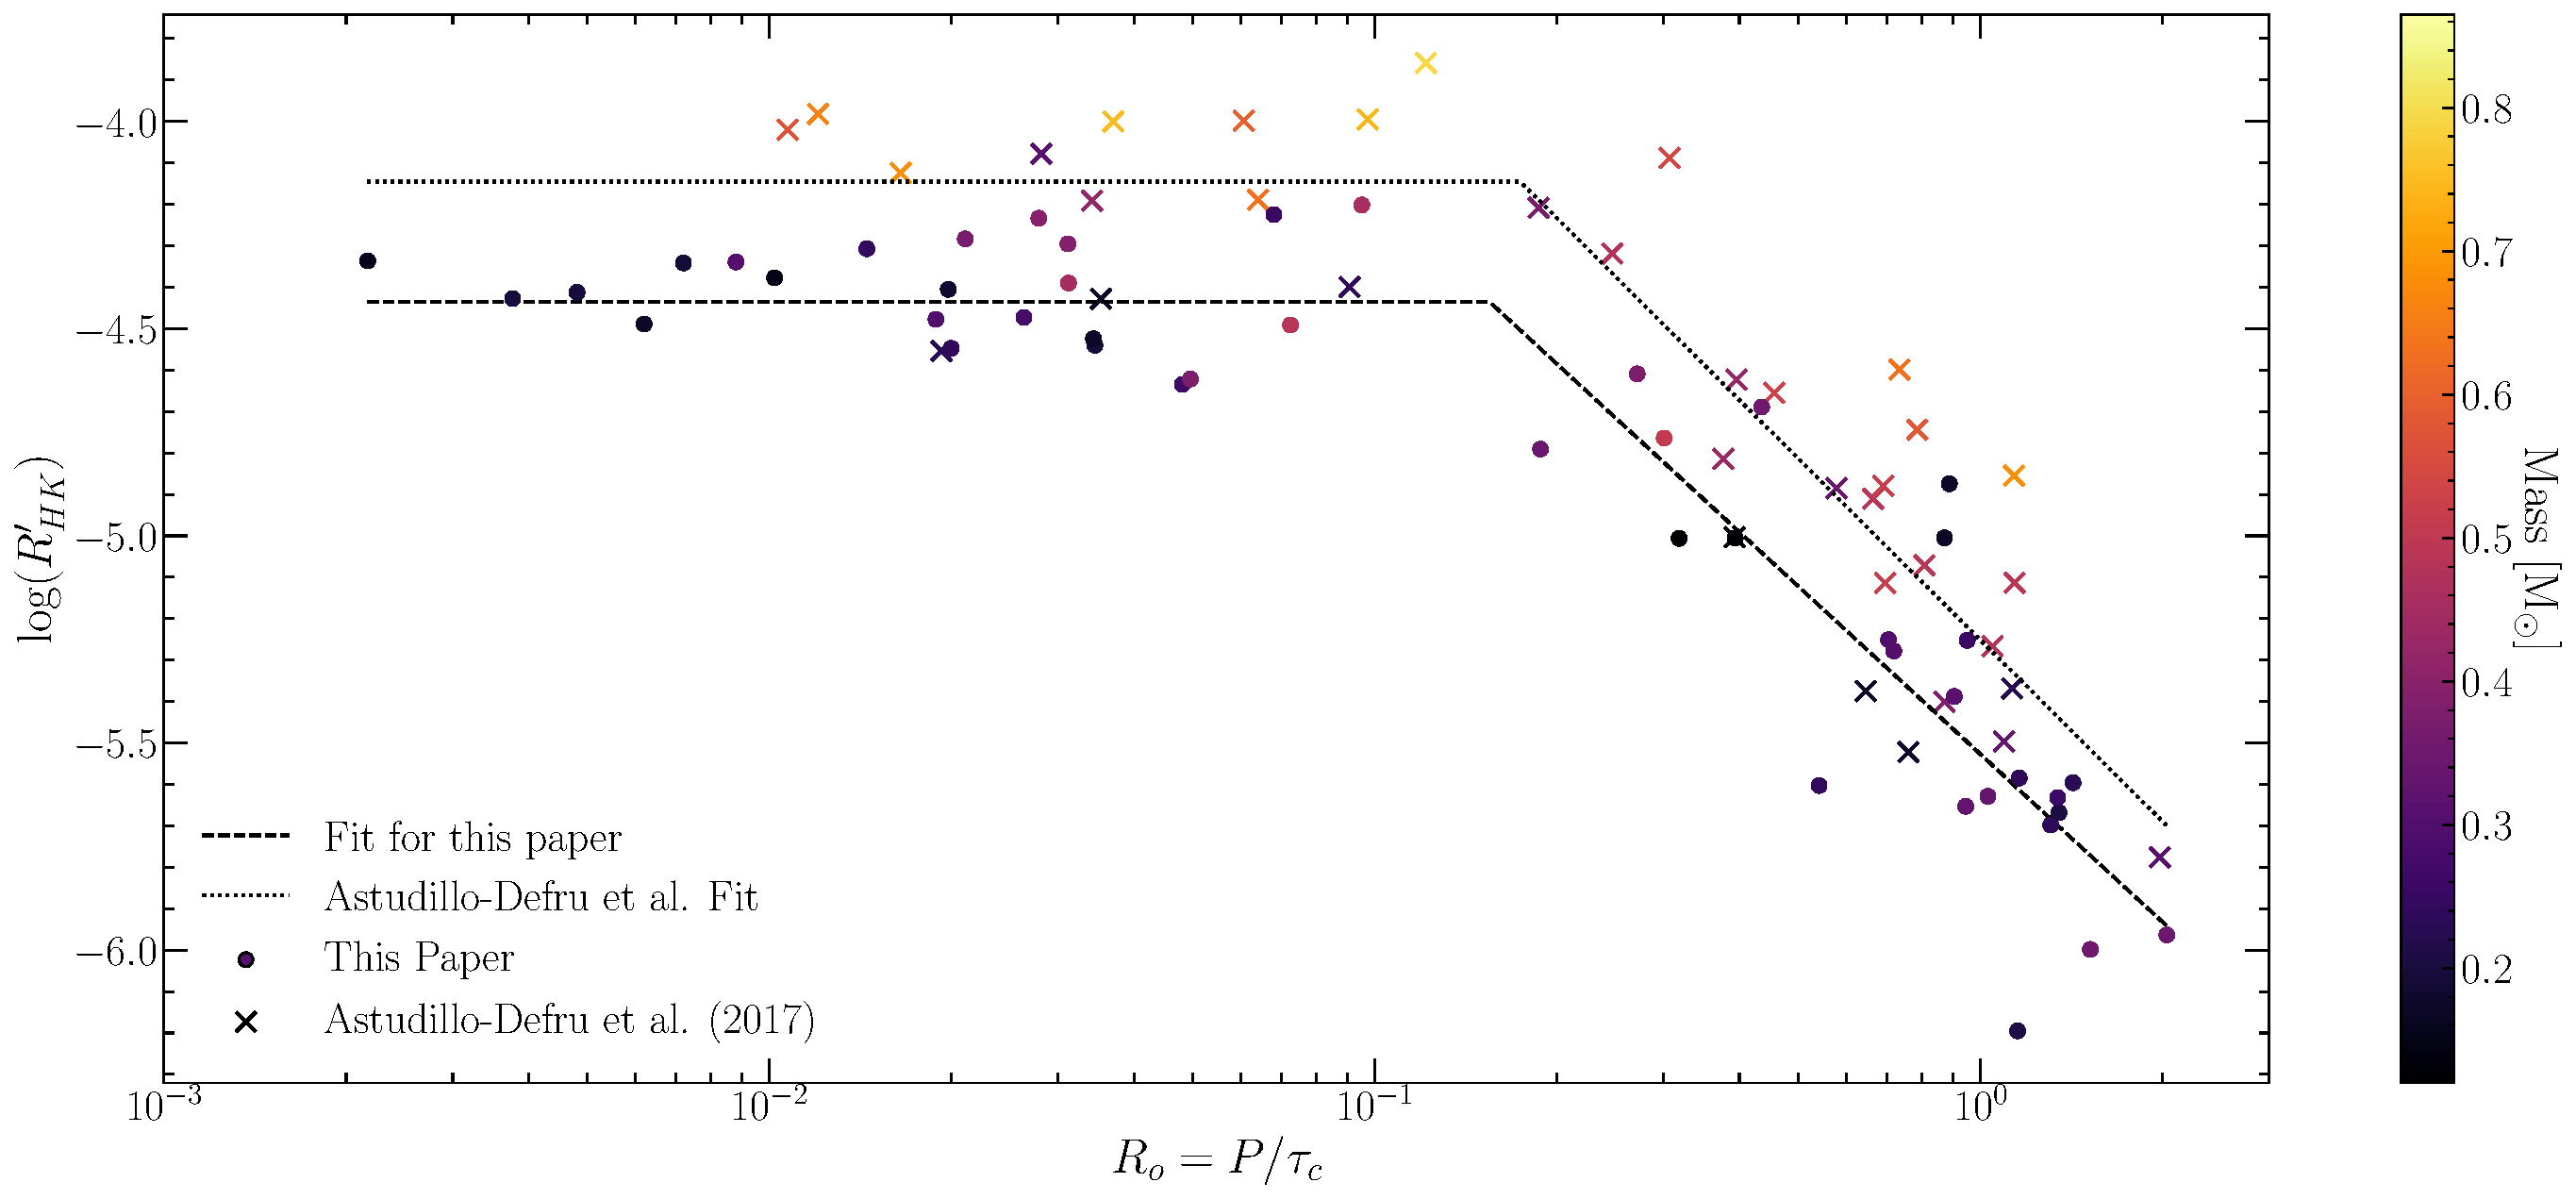
\includegraphics[width=0.9\textwidth]{figures/magActivity/RpHKvsR0_MC.pdf}
	\caption{Rotation activity relation for both our work and \citet{Def17}.
	The dotted line is the best fit to the re-derived rotation-activity
	relation from \citet{Def17}.  Note that targets from \citet{Def17} are
	systematically higher than targets presented here as a consequence of the
	range in mass probed by the samples.}
    \label{fig:RpHKvsRossbyDef}
\end{figure*}
\begin{figure*}
    \centering
    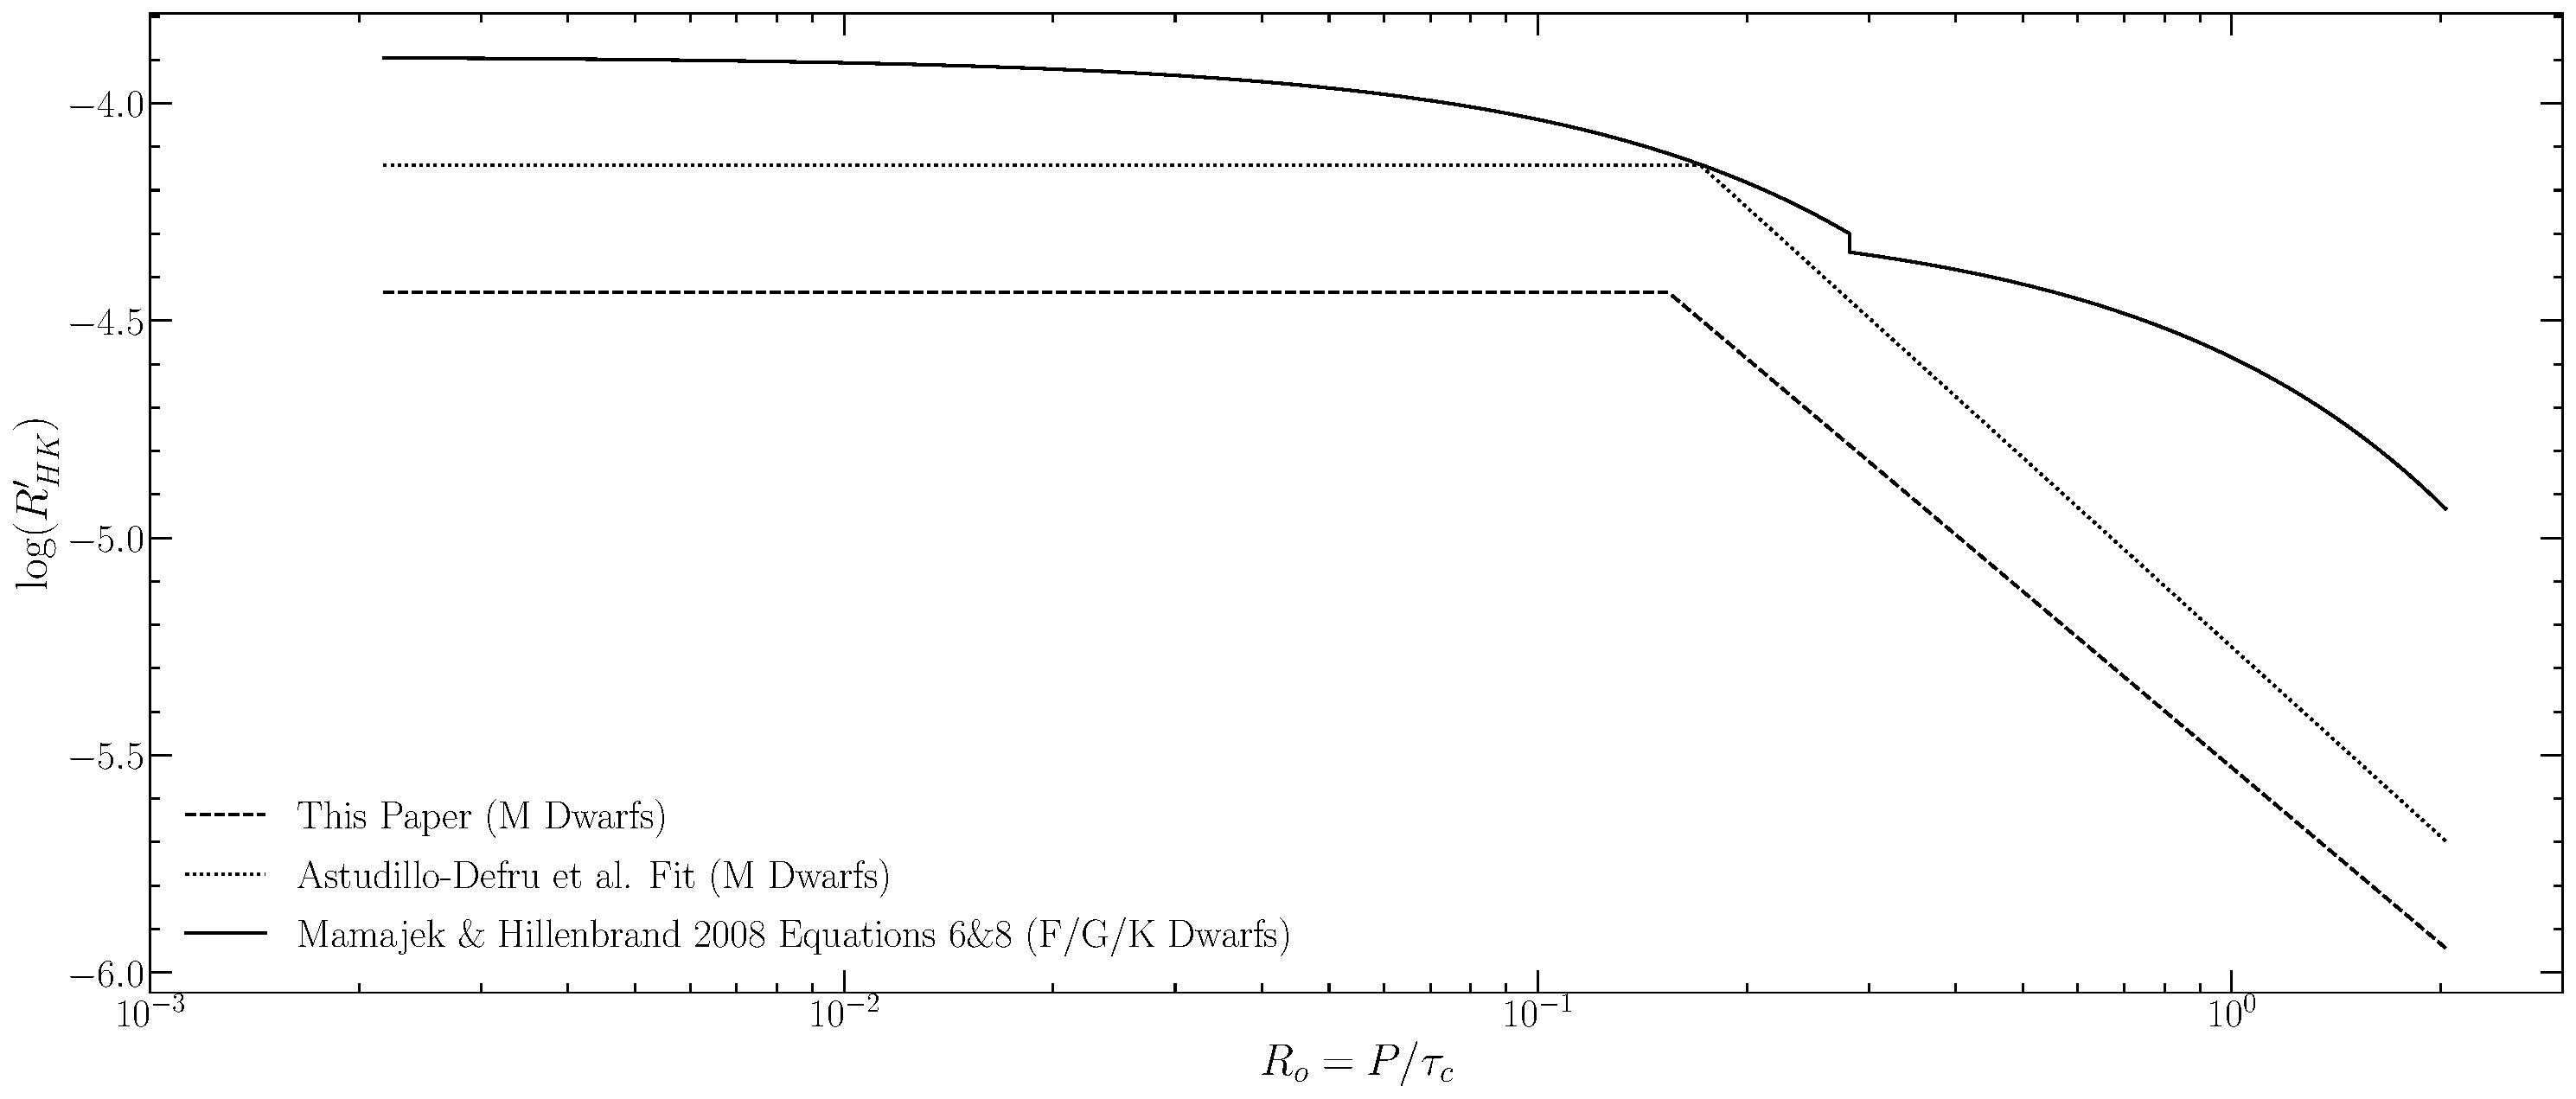
\includegraphics[width=0.9\textwidth]{figures/magActivity/RpHKvsR0_MC_fits.pdf}
	\caption{Derived rotation-activity curves from this work, \citet{Def17} and
	\citet{Mamajek2008}. Note both that \citet{Mamajek2008} focuses their work
	on earlier spectral classes and fits the rotation activity relation in
	linear space.}
    \label{fig:RpHKvsRossbyFits}
\end{figure*}

We find best fit parameters with one $\sigma$ errors:
\begin{itemize}
    \item $k = -1.347\pm 0.203$
    \item $Ro_{s} =  0.155\pm0.045$
    \item $\log(R_{s}) = -4.436\pm0.048$

\end{itemize}
A comparison of the rotation activity derived in this work to those
from both \citet{Def17} and \citet{Mamajek2008} is presented in Figure
\ref{fig:RpHKvsRossbyFits}. For the 6 targets which do not have measured
rotational periods we include an estimate of $Ro$ and $p_{rot}$ in the machine
readable version of Table \ref{tab:finalData}. The convective overturn
timescale for one of these 6 targets (2MASS J13464102-5830117) can not be
inferred via Equation \ref{eqn:convectiveOverturn} as it lacks a V-K color
measurement. Instead, we infer $\tau_{c}$ via \citet{Wri18} Equation 6 (this
paper Equation \ref{eqn:ConvectiveOverturnTimeMass}) using mass. Similar to our
manner of inferring $\tau_{c}$ via color, when inferring $\tau_c$ via mass, we
adopt the larger of the two antisymmetric errors from \citet{Wri18}.

\begin{equation}\label{eqn:ConvectiveOverturnTimeMass}
	\log_{10}(\tau_{c}) = 2.33\pm0.06 - 1.5\pm0.21\left(M/M_{\odot}\right) + 0.31\pm0.17\left(M/M_{\odot}\right)^{2}
\end{equation}

Note that $R'_{HK}$ for one of six of these targets (2MASS
J15165576-0037116) is consistent to within 1$\sigma$ of the saturated value;
therefore, the reported $Ro$ for this target should only be taken as an upper
bound. The remaining five targets have measured $R'_{HK}$ values consistent
with the unsaturated regime. Estimated periods are consistent with previous
constraints. Of the six stars, two were listed as non-detections in
\citet{Newton2018}, and the remaining four as uncertain (possible) detections.
Of the four classed as uncertain, 2MASS 12384914-3822527 and 2MASS
19204795-4533283 have candidate periods $>100$ days and non-detections of
H-alpha emission \citep{Hawley96}. These two stars and the two non-detections
have Ca II H\&K activity levels suggesting very long periods. 2MASS
13464102-5830117 has a candidate period of 45 days, and 2MASS 15165576-0037116
of 0.8 days, both consistent with their higher levels of Ca II H\&K emission.

As a test of the proposed weak correlation between activity and rotation in the
``saturated'' regime seen in some works \citep{Mamajek2008,
Reiners2014, Leh20, Med20} --- though not in others \citep{Wri11, Nunez2015,
Newton2017} ---   we fit a second model whose power law index is allowed to
vary at $Ro < Ro_{s}$. We find a saturated regime power law index of
$-0.052\pm0.117$, consistent with 0 to within 1$\sigma$. Moreover,
all other parameter for this model are consistent to within one $\sigma$ of the
nominal  parameters for the model where the index is constrained to 0 below
$Ro=Ro_{s}$. We can constrain the slope in the saturated
regime to be between -0.363 and 0.259 at the $3\sigma$ confidence level.
Ultimately, we adopt the most standard activity interpretation, a
fully-saturated regime at $Ro < Ro_{s}$. 

We investigate whether our lack of detection of a slope for $Ro <
Ro_{s}$ is due to the limited number of observations in that region when
compared to other works \citep[e.g.][93 targets $Ro < Ro_{s}$]{Med20} through
injection and recovery tests. We inject, fake, rotation-activity measurements
into the saturated regime with an a priori slope of -0.13 --- the same as in
\citeauthor{Med20}. These fake data are given a standard deviation equal to the
standard deviation of our residuals ($12\%$). We perform the same MCMC model
fitting to this new data set as was done with the original data set multiple
times, each with progressively more injected data, until we can detect the
injected slope to the three sigma confidence level. Ultimately, we need more
than 65 data points --- 43 more than we observed in the saturated regime --- to
consistently recover this slope. Therefore, given the spread of our data we
cannot detect slopes on the order of what has previously been reported in the
literature.

We observe a gap in rotational period over a comparable range to the
one presented in \citet{Newton2016} Figure 2. Namely, that M-dwarfs are
preferentially observed as either fast or slow rotators, with a seeming lack of
stars existing at mid rotational periods. This period gap manifests in the
Rossby Number and can be seen in Figure \ref{fig:RpHKvsRossbyDef} as a lack of
our targets near to the knee-point in the fit. This period gap likely
corresponds to that seen by \citet{Browning2010}, who found a paucity of M
dwarfs at intermediate activity levels in Ca II H\&K and note the similarity to
the Vaughn-Preston gap established in higher mass stars \citep{vaughan1980}.
\citet{Magaudda2020} also identify a double-gap in x-ray activity for stars in
the unsaturated regime; it is not clear that the gap we see is related. As a
consequence of this period gap, there exists a degeneracy in our data
between moving the knee-point and allowing the activity level to vary in the
saturated regime.  In the following, we adopt the model of a fully saturated
regime.

We wish to compare our best fit parameters to those derived in \citet{Def17};
however, the authors of that paper do not fit the knee-point of the
rotation-activity relation. They select the canonical value for the rotational
period separating the saturated regime from the unsaturated regime ($P_{rot,s}
= 10$ days) and use a fixed convective overturn timescale ($\tau_{c} = 70$
days). To make our comparison more meaningful we use the $P_{rot}$ and $V-K$
colors presented in \citet{Def17} to re-derive $Ro$ values using $\tau_{c}$
\citep{Wri18}. Doing this for all targets presented in \citet{Def17} Table 3
and fitting the same piecewise power law as before, we find best fit parameters
of $Ro_{s} = 0.17\pm0.04$, $\log(R_{s}) = -4.140\pm0.067$, and
$k=-1.43\pm0.21$. Compared to the best fit parameters for our data, $Ro_{s}$
and the unsaturated regime's index, $k$, are consistent to within one sigma,
while the saturated value, $R_{s}$, differs. 

The mass ranges of our respective samples explain the differences in saturation
values between our work and that of \citet{Def17}. Our work focuses on
mid-to-late M-dwarfs and includes no stars above a mass of $0.5$ M$_{\odot}$
(Figure \ref{fig:massDistribution}).  The strength of Ca II H\&K
emission is known to decrease as stellar mass decreases \citep{Schrijver1987,
Rauscher2006, Hou17}. As \citet{Rauscher2006} note, this is the opposite as the
trend seen in H-alpha; the latter primarily reflects the increasing length of
time that lower M dwarfs remain active and rapidly rotating \citep{West2015,
Newton2016}.

A mass dependence can be seen in Figure 10 in \citet{Def17}, consistent
with expectations from the literature. If we clip the data from \citet{Def17}
Table 3 to the same mass range as our data-set ($M_{*} < 0.5M_{\odot}$) and fit
the same function as above, we find that all best fit parameters are consistent
to within one sigma between the two data-sets. 

\begin{figure}
    \centering
    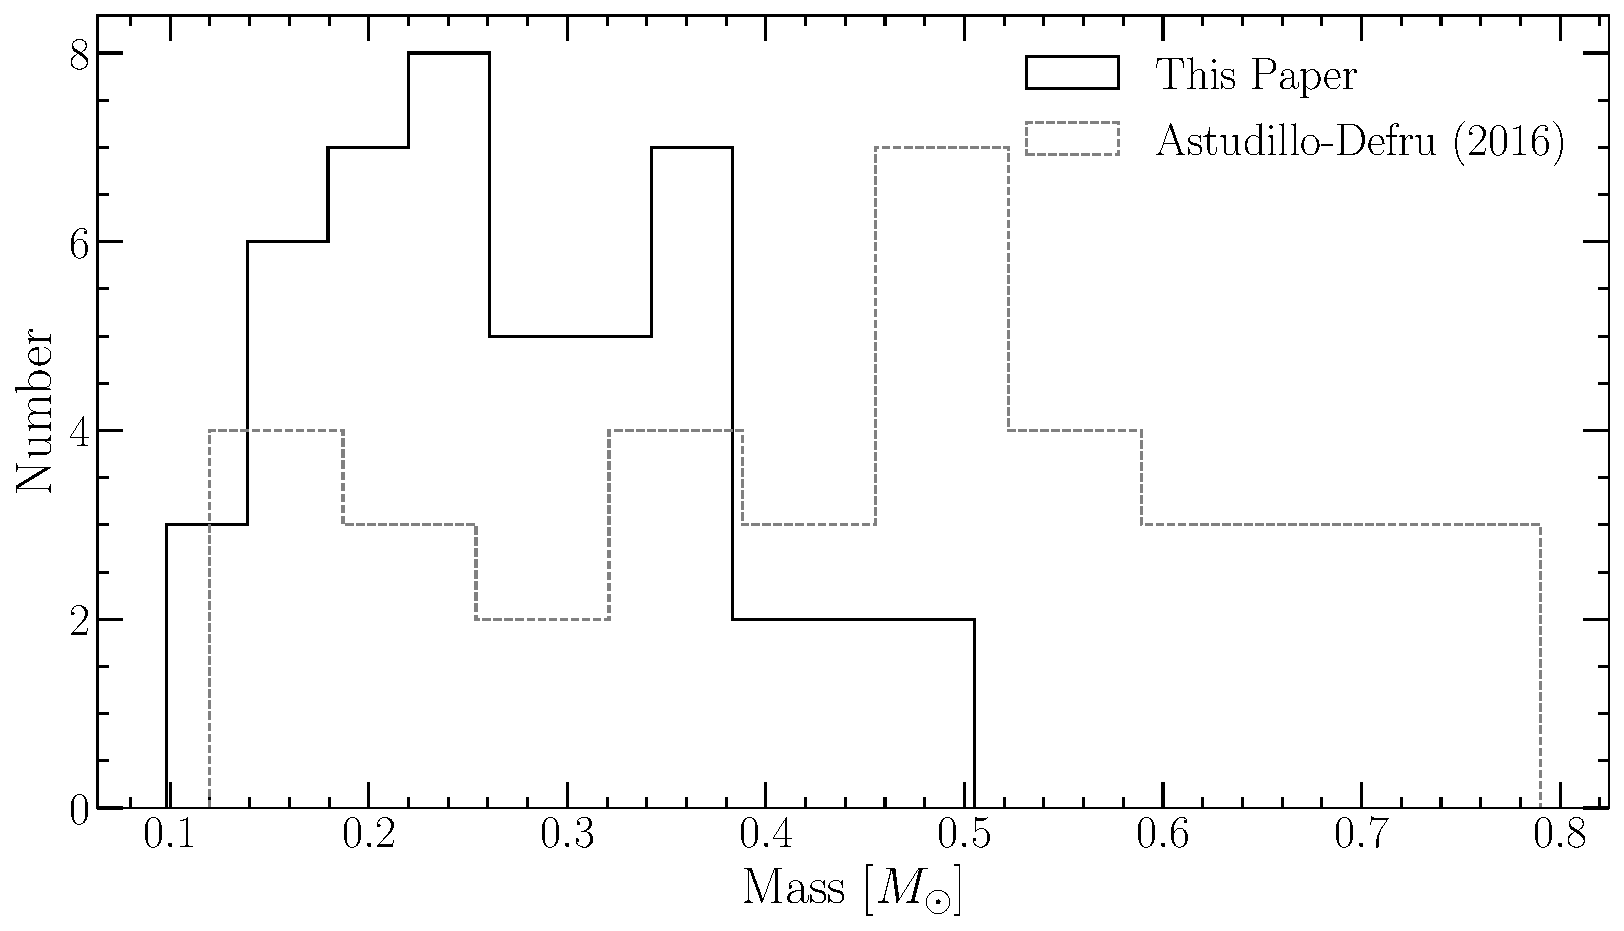
\includegraphics[width=0.85\textwidth]{figures/magActivity/B2020vsAD2016_Masses.pdf}
	\caption{Distribution of masses between our sample and the sample presented
	in \citet{Def17}. Note how the two studies have approximately the same
	sample sizes; however, our sample is more tightly concentrated at lower
	masses \textbackslash later spectral classes.}
    \label{fig:massDistribution}
\end{figure}

We also compare our best fit $Ro_{s}$ to both those derived in
\citet{Newton2017} using $H_{\alpha}$ as an activity measure and those derived
in \citep{ Wri18, Magaudda2020} using $L_{X}/L_{bol}$ as an activity measure.
Works using $L_{X}/L_{bol}$ identify a similar, yet not consistent to within
one sigma result for $Ro_{s}$; while, the value of $k$ we find here is
consistent between all four works. Therefore, we find similar results not only
to other work using the same activity tracer, but also a power-law slope that
is consistent with work using different tracers. 

\section{Magnetic Activities in M dwarfs Closing Thoughts}\label{sec:magActivity-conclusions}
In this work we have approximately doubled the number of M-dwarfs with both
empirically measured $R'_{HK}$ with $M_{*} < 0.5 M_{\odot}$. This has enabled
us to more precisely constrain the rotation-activity relation. This
relationship is consistent with other measurements using $R'_{HK}$, and
$L_{X}$/$L_{bol}$; our data does not require a slope in the saturated regime.
Finally, we identify a mass dependence in the activity level of the saturated
regime, consistent with trends seen in more massive stars in previous works.



\chapter{The Red Giant Branch Bump}
The red giant branch bump (RGBB) is a feature experienced by many stars as they ascend the RGB. During this period, as the core of
the star is contracting and heating the surronding matierial shell burning
begins. Regions of the star which were previously too cool to fuse hydrogesn
(and so therefore still have hydrogen fuel despite core depletion) begin to
fuse. At the same time, because of the increase energy output from the heating
core and shell burning the balance between the adiabatic and radiative
temperature gradients near the convective envlope of the star begins to flip.
This results in the convective envelope pushing deeper --- in mass fraction --- into the star. As the
convective envelope reaches further into the star hydrogen from the stars outer
layers may be effeciently mixed deeper. The convective envelope only ever
manages to reach a fraction of a stars mass fraction during this phase of evolution;
however, due to the efficient mixing, by the time it starts to recede to the
surface there is a radial discontinuity in the hyrdogen concentration within
the star. If shell burning reaches this far out then the normal corse of RGB
asension will be interupted by an anoumously large amount of fuel. The star
will remain burning that shell for longer than might otherwise be predicted
leading to a ``bump'' in the luminosity function. This is known as the Red
Giant Branch Bump.

The RGBB provides yet another view into the interior physics of a star and may
allow for calibration and testing of stellar models against observations.
Previous work by \citet{Joyce2016} has found that current
generation 1D stellar models, such as DSEP, may undersestimate the bump
luminosity for metal poor stars but that they generally models the bump well
for more metal rich stars.

In this chapter we will provide two breif views into the RGBB. First, we will
look at how different self consistent models of multiple populations in NGC
2808 (the same models disscused in Chapter \ref{chap:ngc2808}) effect the
RGBB location. Second, we will investigate how the updated low and high
temperature opacities which we have incorperated into DSEP effect the RGBB
location.

\section{The Red Giant Branch Bump in NGC 2808}
NGC 2808 is made up of of anywhere from 2 - 5 separate stellar populations. In
Chapter \ref{chap:ngc2808} we discussed modeling efforts of the primordial
and the most enriched of these populations (A and E). Here we identify the
RGBB location in both populations and compare that to observations of the RGBB
luminosity.

Identification of the RGBB may be performed with either isochrones or stellar
evolutionary tracks. For the same reasons laid out in \citet{Joyce2016} we use
evolutionary tracks in place of isochrones. This is primarily due to the
limited sampling of equivalent evolutionary points near the bump which can
result in the bump be interpolated over. 

We select two evolutionary tracks from the Population A (Y $\sim$ 0.24) and
Population E (Y $\sim$ 0.36) model sets each of a mass so that they reach the
red giant branch within 100 Myr of each other. The population A model is of
mass 0.857 M$_{\odot}$ while the population E model is of mass 0.625
M$_{\odot}$. Identification of the RGBB in the tracks is then straightforward.
First we perform bolometric corrections to take the tracks into WFC3/ACS
filters with the same distance modulus and extinction as we fit in Chapter
\ref{chap:ngc2808}, then we identify the maximum of the derivative of F814W
magnitude vs. age. This metric proves to reliably extract the center of the
RGBB. We identify the bump in population A at an F814W magnitude of approximately 16.5 while
we are unable to identify the gap in population E.

In order to verify this is a attribute of the population and not the particular
model we selected we perform stellar population synthesis using the best fit
isochrones from Chapter \ref{chap:ngc2808}. This is done using the population
synthesis module in \fidanka. Further, HUGS artificial star tests are used in
order to inject proper uncertainties and to model completeness. Figure
\ref{fig:LumFAE} shows both the synthetic population (left) and the luminosity
function of that population (right). We measure the magnitude of the RGBB by
first flattening the luminosity function shown in Figure \ref{fig:LumFAE} with
a second order polynomial. We then fit a Gaussian model --- with a prior of
16.5 as the mean of the RGBB magnitude --- to the flattened luminosity function.
We find that the RGBB in population A is located at F814W = 16.53$\pm$0.004
mag, this is in agreement with literature values for the magnitude of the RGBB
in NGC 2808. However, once again we do not see a bump in the synthetic
population E data. The pertinent question then becomes why do we not see a
RGBB in population E when compared to population A.

\begin{figure}
  \centering
  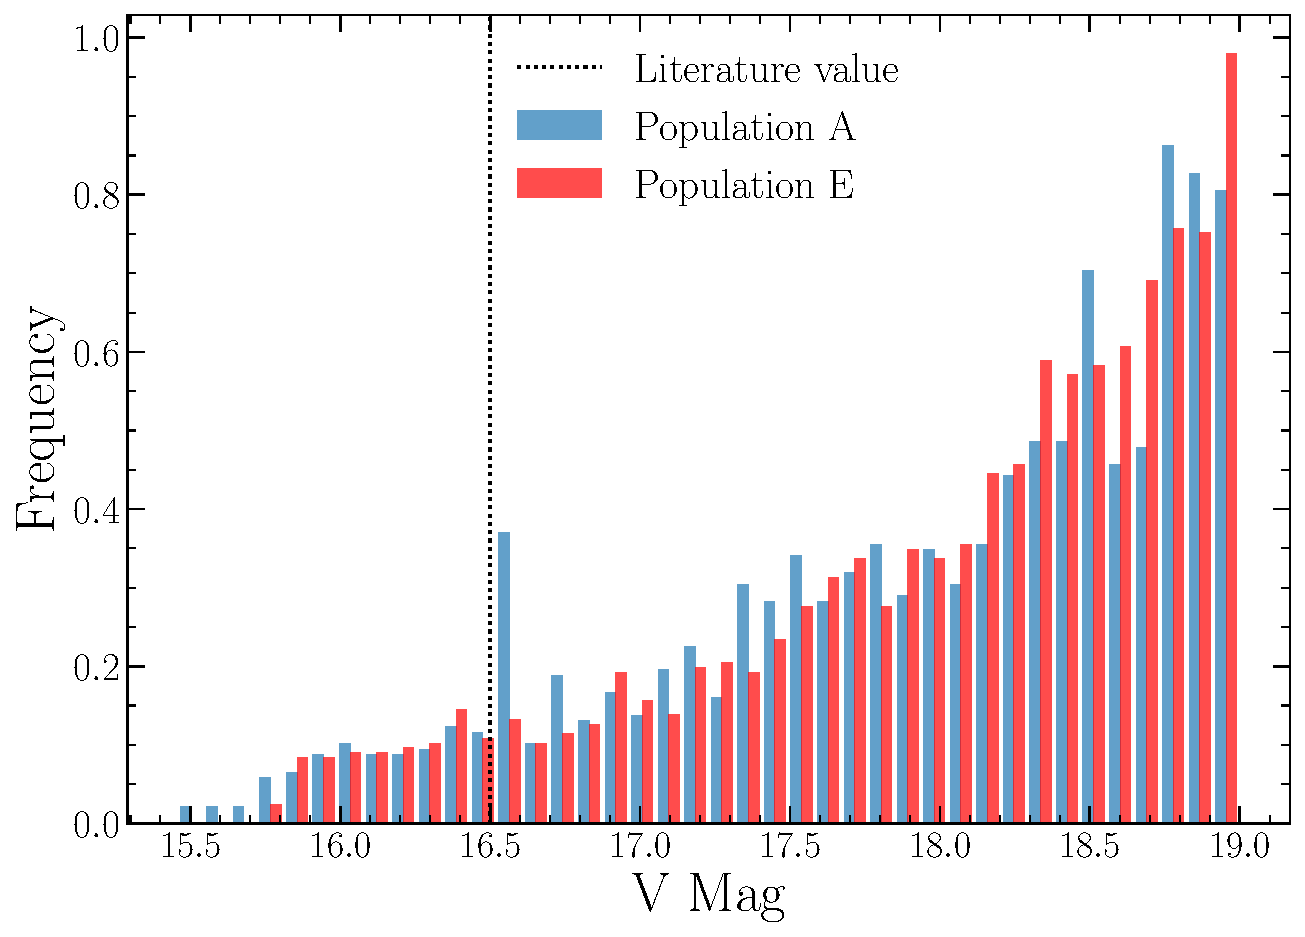
\includegraphics[width=0.85\textwidth]{figures/rgbb/ComparisonOfRGBBump.pdf}
  \caption{Luminosity function for a population A and E model. Note how there
  is a bump at approximately $M_{V} = 16.5$ for population A but not for E. The
  dashed line represents the literature value for the observed RGBB in NGC
  2808.}
  \label{fig:LumFAE}
\end{figure}

\subsection{Population E and the Case of the Missing Bump}
It is well established that stars with lower metallicities will have a less
pronounced bump \citep{Cassisi2002, Bjork2006}. Due to Population E's
signifigantly enhances helium abundance the mean molecular mass ($\mu$) within
population E stars is approximatly 25\% larger than $\mu$ is for population A
stars. Higher mean mollecular masses steepen the adiabatic temperaure gradient
thus changing the depth at which a model is unstable to convection. Moreover,
the metallicity of population E is lower than that of population A. Lower
metallicities decrease the opacity of a star and therefore make the coupling
between the radiation field and the fluid field weaker. This results in less
efficient thermal transfer into the fluid of the star. Consequently, models have
a more shallow outer convective zone (Figures \ref{fig:convEnvMass} \&
\ref{fig:MfracVX}) which may not be able mix new hydrogen fuel both deep enough
within a model and early enough in a model's life to induce the RGBB.
Specifically, in population E we see that the convection zone only reaches down
50\% of the mass of the model (Figure \ref{fig:MfracVX}). Because of this,
shell burning does not reach the discontinuity in hydrogen mass fraction until
later in the model's life. Because the luminosity of the models is rapidly
increasing during this phase of evolution the timescales to burn hydrogen
shrink rapidly as well. Therefore, in population E even though there does seem
to be a small discontinuity in the hydrogen mass fraction, evolutionary time
scales are so short that the population will evolve through this period without
a noticeable bump. The lack of an observed RGB bump in Population E models ---
and the commensurate lack of effect that population E has on the location of
the NGC 2808 bump --- validates previous theoretical investigations of the bump
which have ignored the presence of multiple populations in NGC 2808 while
modeling the bump.

\begin{figure}
  \centering
  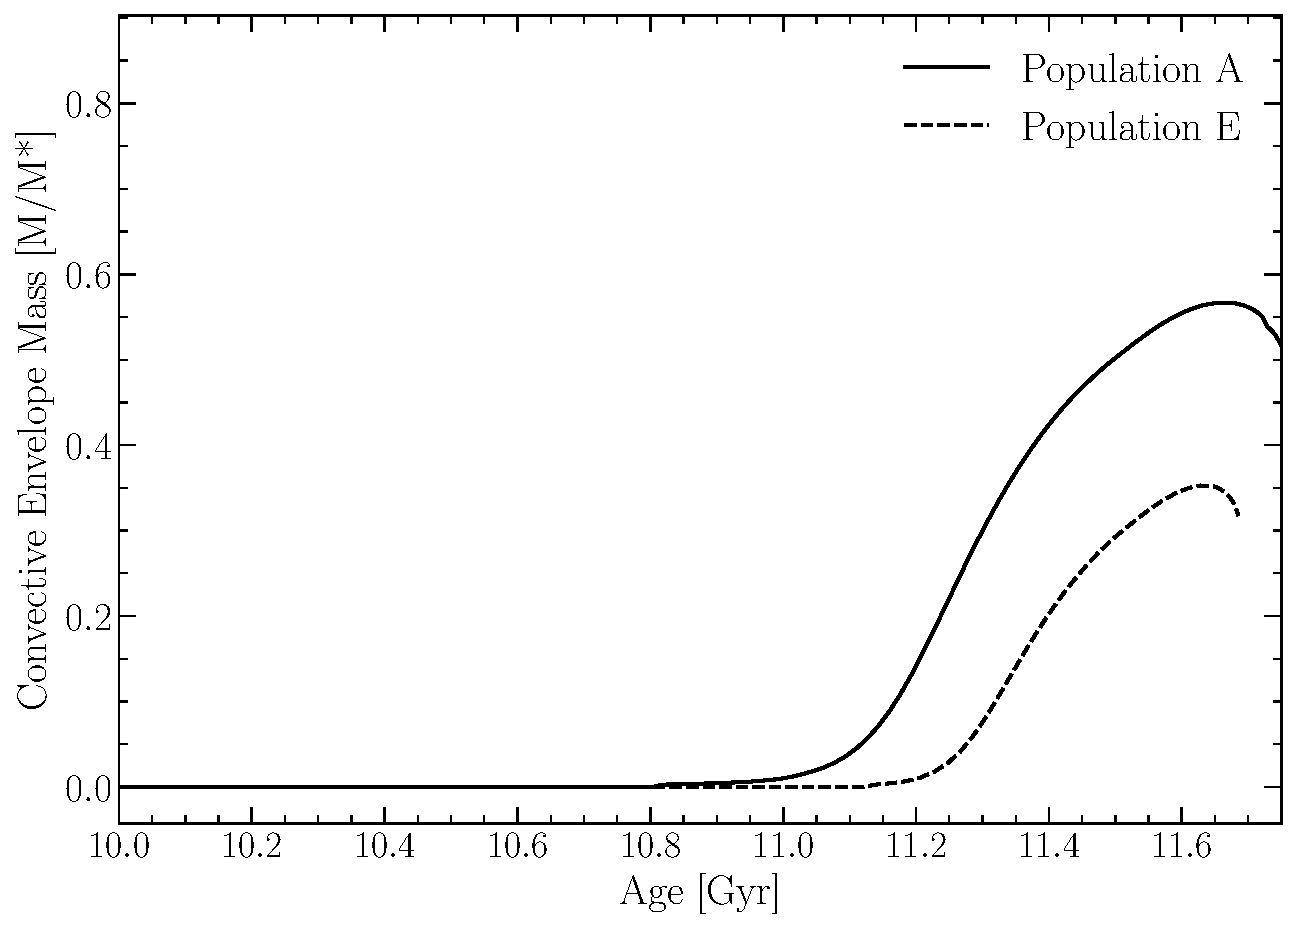
\includegraphics[width=0.85\textwidth]{figures/rgbb/ConvectiveEnvelopeMass.pdf}
  \caption{Fractional mass of the convective envelope of a population A and E
  model vs. model age. Note how the population A model's convective envelope
  reaches approximately 60 percent of the star by mass while the population E
  convective envelope only reaches 40 percent of the star by mass.}
  \label{fig:convEnvMass}
\end{figure}

\begin{figure}
    \centering
    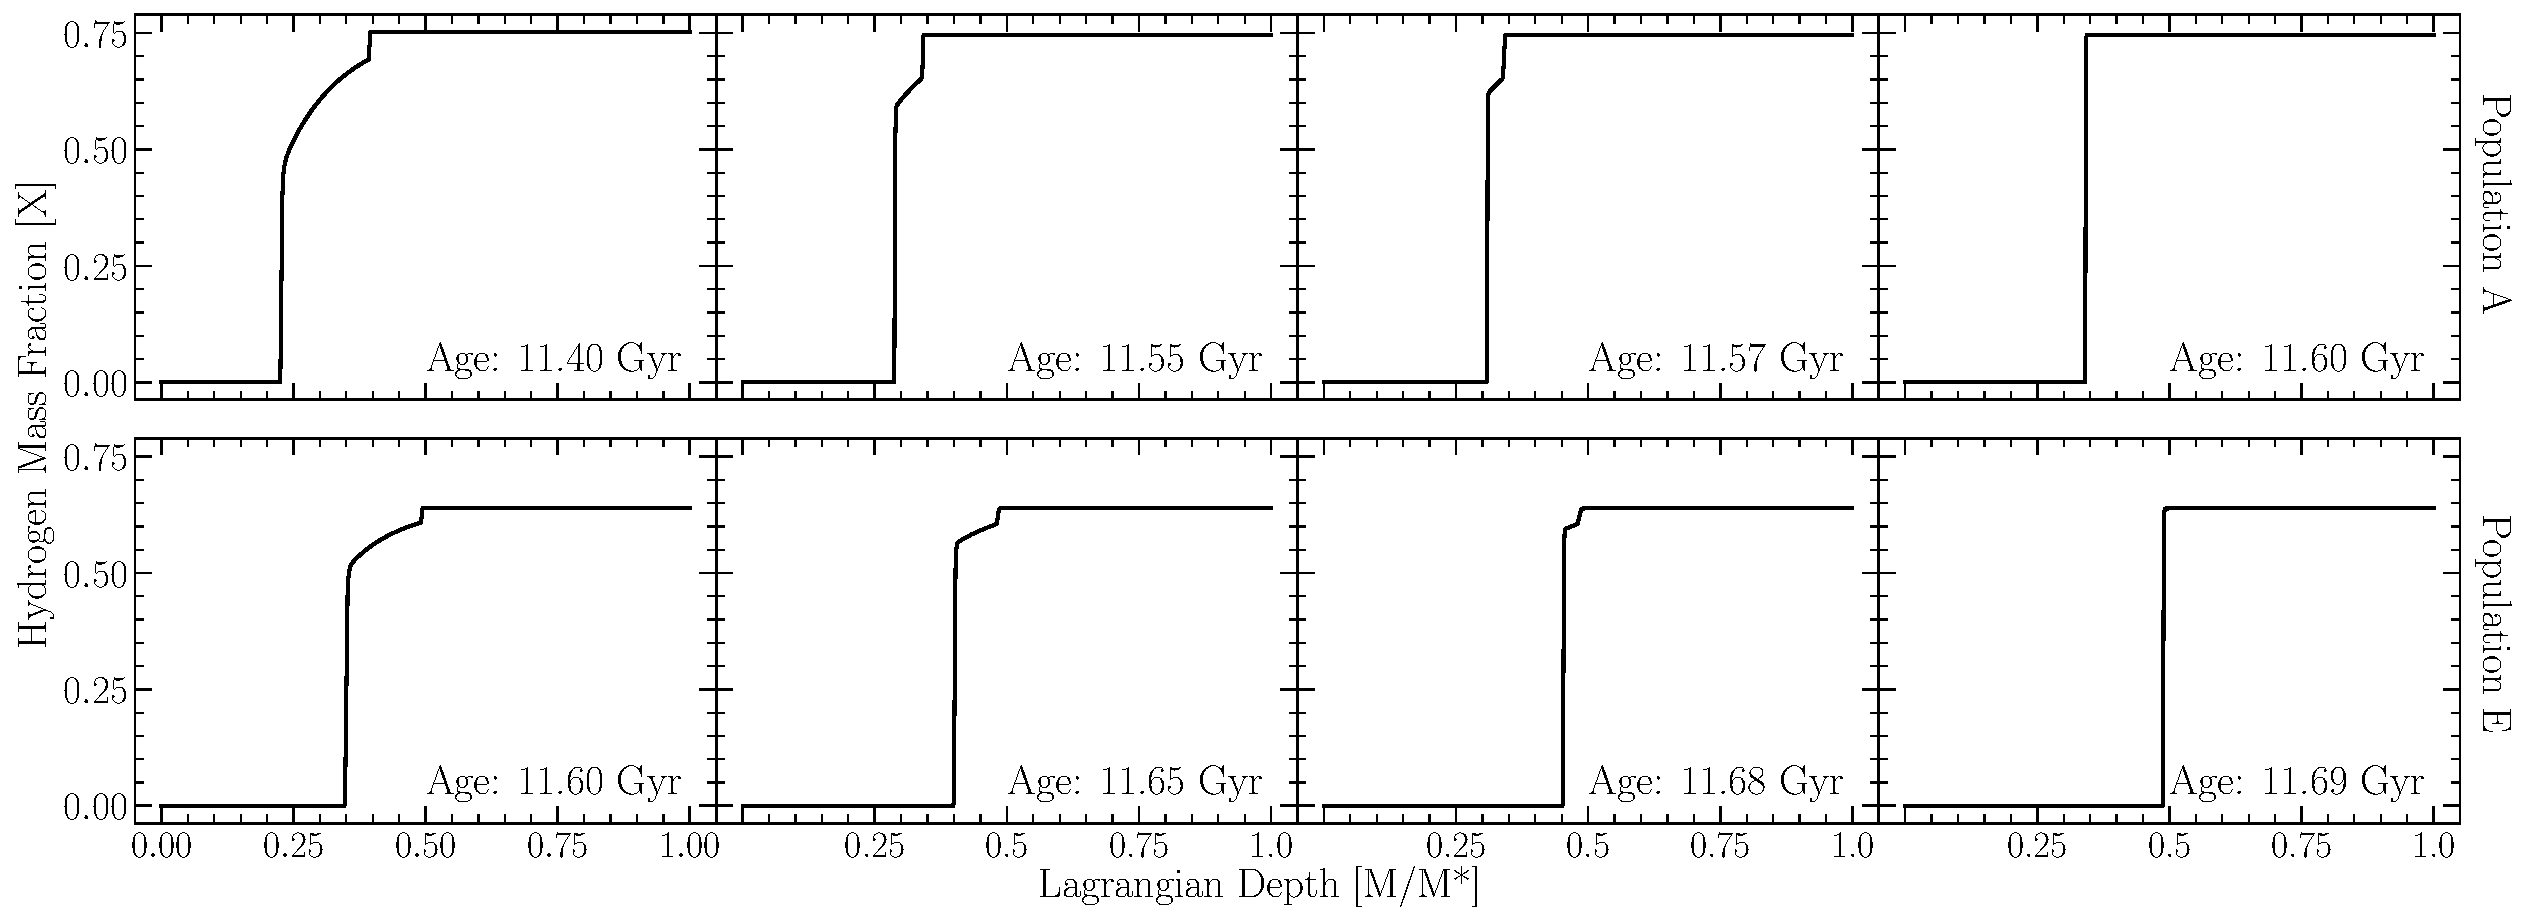
\includegraphics[width=\textwidth]{figures/rgbb/EvolutionAE.pdf}
    \caption{Evolution of the hydrogen mass fraction vs. the Lagrangian depth
    within Population A (top) and E (bottom) Stellar models. From left to right
    panels show snapshots at informative ages. Note how Population E does not
    exhibit the same deep bump in its hydrogen mass fraction as Population A
    does. Populations have been roughly mas calibrated so they reach the same
    evolutionary stages within 100 Myr of each other.}
    \label{fig:MfracVX}
\end{figure}

\section{Effects of Opacities on the Red Giant Branch Bump}
In addition to models of multiple populations in NGC 2808, we also have access
to GS98 solar composition models using OPAL and Ferguson opacities as well as
models using OPLIB and Aesopus opacities (high and low temperature
respectively). Given the RGB bumps sensititvity to convective zone depth, as
demonstrated in the previous section, it is reasonable to assume that
variations in the opacity may have an effect on its location. 

Following the procedure outlined in \citep{Joyce2016} we identify the RGB Bump
in models evolved over an [Fe/H] grid of -2.0, -1.8, -1.6, -1.4, -1.2, -1.0,
and -0.8. All models use a GS98 solar composition, high temperature opacities
from OPLIB and low temperature opacities from Aesopus. Models are evolved with
a typical numerical tolerance of one part in 10$^{5}$ and include gravitational
settling. All other model parameters are the same as outlined in Chapter \ref{chap:ngc2808}. 

The evolutionary tracks for each model are bolometrically corrected into
UBV(RI)c filters using the bolometric correction tables provided by MESA
\citep{Choi2016} and \fidanka. These bolometric corrections additionally assume $\mu =
0$ and $A_{v} = 0$. The magnitude of the bump is then defined as the magnitude
at the age where the magnitude-age derivative is maximized. We visually inspect
all models to confirm that the identified magnitude aligns with the location of
the bump.

Comparing bump locations between OPAL+Ferguson opacities (Figure
\ref{fig:OPALvsOPLIBRGBB}) to OPLIB+Aesopus opacities we find that indeed the
updated opacities to effect the location of the bump; however, this is a very
small effect, on the order of a few parts in 100. Given that the updated
opacities have such a small effect on the RGBB location, and do not resolve the
discrepancies seen in \citet{Joyce2016} we do not believe that a more detailed
investigation of the effects opacity have on RGBB location in warranted.

\begin{figure}
  \centering
  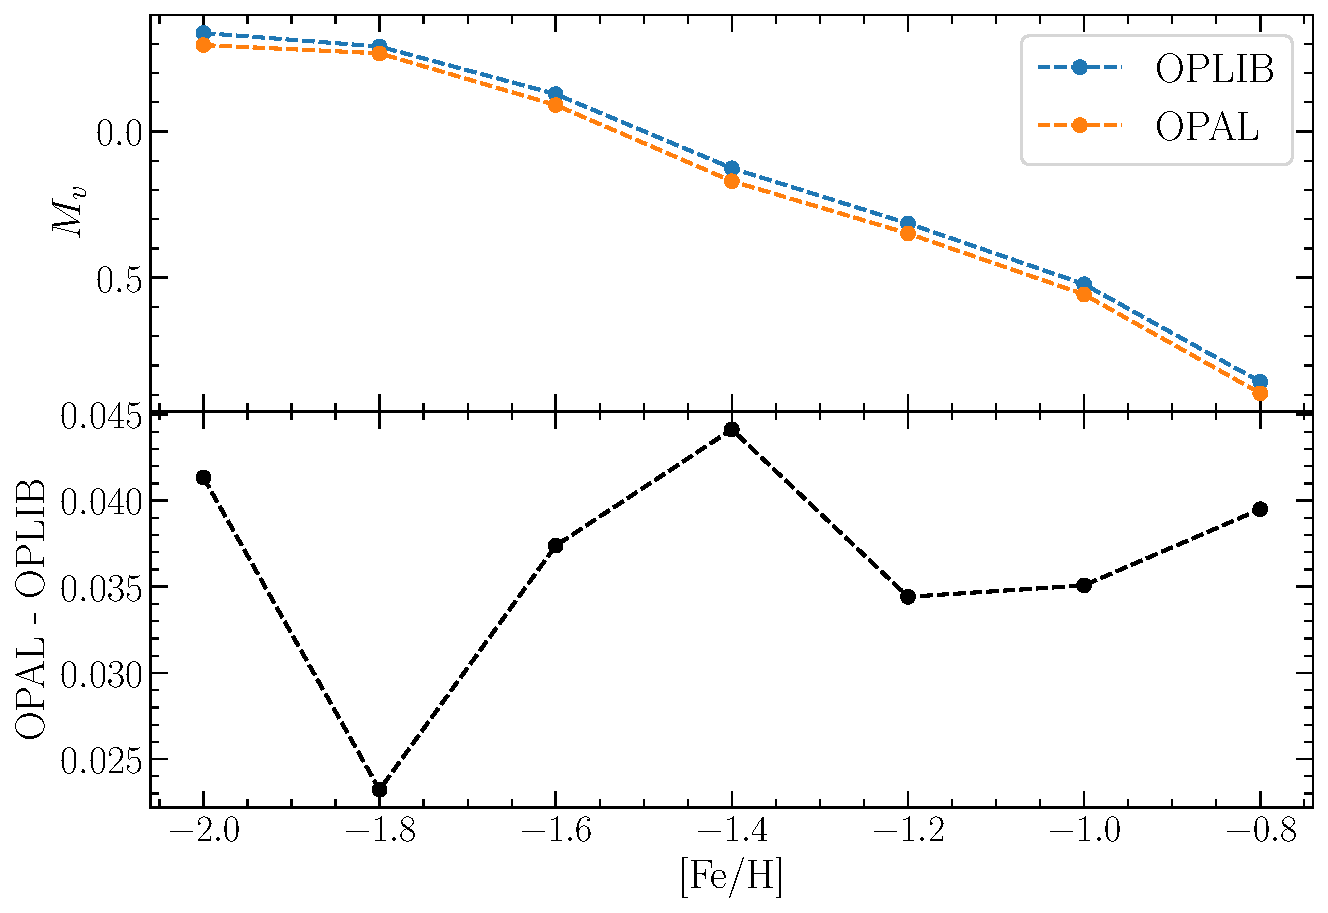
\includegraphics[width=0.85\textwidth]{figures/rgbb/OPALvsOPLIBComparison.pdf}
  \caption{V magnitude of the red giant branch bump as predicted by models
  evolved with OPAL+Ferg opacities and models evolved with OPLIB+Aesopus
  opacities. The updated opacities tend to push the bump to slightly smaller
  magnitudes; however, this is a very weak effect.}
  \label{fig:OPALvsOPLIBRGBB}
\end{figure}




\part{Conclusions}
\section{Conclusion}\label{sec:conclusion}
It is, at this point, well established that the Jao Gap may provide a unique view of the interiors of stars for which other probes, such as seismology, fail. However, it has only recently become clear that the Gap may lend insight into not just structural changes within a star but also into the magnetic environment of the star.
\citet{Jao2023} presented evidence that the physics driving the Gap might additionally result in a paucity of H$\alpha$ emission. These authors propose potential physical mechanisms which could explain this paucity, including the core of the star acting as an angular momentum sink during mixing events.

Here we have expanded upon this work by probing the degree and variability of
Calcium II H\&K emission around the Jao Gap. We lack the same statistical
power of \citeauthor{Jao2023}'s sample; however, by focusing on the
star-to-star variability within magnitude bins we are able to retain
statistical power. We find that there is an anomalous increase in variability
at a G magnitude of $\sim 11$. This is only slightly below the observed mean gap magnitude.

Additionally, we propose a simple model to explain this variability. Making the
assumption that the periodic convective mixing events will have some small but
random effect on the overall magnetic field strength we are able to
qualitatively reproduce the increase activity spread in a synthetic population
of stars. 


\cleardoublepage
\phantomsection
\addcontentsline{toc}{part}{Bibliography}
\bibliography{bib/ms} % Entries are in the refs.bib file
\bibliographystyle{aasjournal} % We choose the "plain" reference style


% Now the user can start typing
\end{document}
